\documentclass[11pt, openany]{book}
\usepackage[text={4.65in,7.45in}, centering, includefoot]{geometry}
\usepackage{multirow}
\usepackage{multicol}
\usepackage{setspace}
\usepackage{ragged2e}
\usepackage{longtable}
\usepackage[table, x11names]{xcolor}

\usepackage{fontspec,realscripts}
\usepackage{polyglossia}

\setdefaultlanguage{sanskrit}
\setotherlanguage{english}
\defaultfontfeatures[Scale=MatchUppercase]{Ligatures=TeX}

\newfontfamily\sanskritfont[Script=Devanagari]{Shobhika}
\newfontfamily\englishfont[Language=English, Script=Latin]{Linux Libertine O}
\newfontfamily\sanskritfont[Script=Devanagari, Scale=0.9]{Shobhika}
\newfontfamily\englishfont[Language=English, Script=Latin]{Linux Libertine O}
\newfontfamily\en[Language=English, Script=Latin, Scale=1.1]{Linux Libertine O}
\newfontfamily\bd[Script=Devanagari, Scale=1]{Shobhika-Bold}
\newfontfamily\bt[Script=Devanagari, Color=violet, Scale=0.9]{Shobhika-Bold}
\newfontfamily\bs[Script=Devanagari, Color=purple]{Shobhika-Bold}
\newfontfamily\ex[Script=Devanagari, Color=red]{Shobhika-Bold}
\newfontfamily\qt[Script=Devanagari, Scale=0.9, Color=violet]{Shobhika-Regular}
\newfontfamily\bqt[Script=Devanagari, Scale=1, Color=brown]{Shobhika-Regular}
\newfontfamily\s[Script=Devanagari, Scale=0.9]{Shobhika-Regular}
\newfontfamily\q[Script=Devanagari, Scale=1, Color=violet]{Shobhika-Bold}
\newcommand{\devanagarinumeral}[1]{%
   \devanagaridigits{\number\csname c@#1\endcsname}}
\usepackage{fancyhdr}
\pagestyle{fancy}
\renewcommand{\headrulewidth}{0pt}
\usepackage{enumerate}
%\pagestyle{plain}
\usepackage{afterpage}
\usepackage{amsmath}
\usepackage{amssymb}
\usepackage{graphicx}
\usepackage{longtable}
\usepackage{footnote}
%\usepackage{dblfnote}
\usepackage{xspace}
%\newcommand\nd{\textsuperscript{nd}\xspace}
\usepackage{array}
\usepackage{emptypage}
\usepackage{hyperref}   % Package for hyperlinks
\hypersetup{
colorlinks,
citecolor=black,
filecolor=black,
linkcolor=blue,
urlcolor=black
}
\begin{document}
\onehalfspacing
{\fancyhead[RE]{\textbf{बीजपल्लवे}}}
{\fancyhead[LO]{\textbf{कुट्टकविवरणम्}}}
{\fancyhead[RO,LE]{\textbf{\thepage}}}
\cfoot{}
\renewcommand{\thepage}{\devanagarinumeral{page}}
\setcounter{page}{123}
\begin{quote}
    \bs
    एवं तदर्धं च तदाधिमासा- \\

\vspace{-7mm}
\hspace{1cm} वमाग्रकाभ्यां दिवसारवीन्द्वोः~॥~३७~॥
\end{quote}
 
 अस्यार्थं स्वयम् एव विवृणोति~। ग्रहस्य विकलाशेषात् ग्रहाहर्गणयोरानयनम्~। तत्र षष्टिर्भाज्यः कुदिनानि हारः विकलावशेषं शुद्धिरिति प्रकल्प्य
गुणाप्ती साध्ये~। तत्र लब्धिः विफलाः स्युर्गुणस्तु कलावशेषम्~। एवं
कलावशेषं शुद्धिं प्रकल्प्य तत्र लब्धिः कलाः गुणो भागशेषं~। भागशेषं
शुद्धिस्त्रिंशद्भाज्यः कुदिनानि हारस्तत्र फलं भागः गुणो राशिशेषम्~। द्वादश भाज्यः 
कुदिनानि हारः राशिशेषं शुद्धिस्तत्र फलं गतराशयः गुणो भगणशेषम्~। 
एवं कल्पभगणा भाज्यः~। कुदिनानि हारः~। भगणशेषं शुद्धिः~। फलं गतभगणाः~। गुणः अहर्गणः स्यादिति~। अस्योदाहरणानि प्रश्नाध्याये~। एवं 
कल्पाधिमासा भाज्यः रविदिनानि हारः अधिमासं शेषं शुद्धिः फलं गताधिमासाः~। 
गुणो गतरविदिवसाः~। एवं युगावमानि भाज्यश्चन्द्रदिवसाः हार अवमशेषं 
शुद्धिः फलं गतावमानि गुणो गतचान्द्रदिवसा इति~। अत्राचार्यव्याख्याने 
युगावमानि भाज्य इत्यत्र कल्पशब्दस्तेन युगेति लिखनं लेखकभ्रमजं द्रष्टव्यं यद्वा 
न केवलं कल्पजैर्भगणकुदिनाधिमासावमादिभिर्ग्रहाहर्गणाद्यानयने
विकलाशेषादेस्तदानयनं किन्तु युगजैरपि कुदिनाद्यैस्तत्साधने
तदुत्पन्नाद्विकलाशेषाद्युगजभाज्यभाजकेभ्योऽपि तत्साधनं भवतीति सूचनाय युगावमानीत्युक्तम्~। एवं यथा सम्भवं युगचरणजैरपि कुदिनादिभिर्ग्रहादिसाधने तादृशभाज्यभाजकेभ्यः कुट्टको ज्ञेयः~। अत एव सूत्रे कुदिनानि हार इत्येवोक्तं न तु कल्पकुदिनानीति~। अत्र मन्दप्रतीत्यर्थं कल्पितानि कल्पकुदिनानि १९ ग्रहभगणाः कल्पे कल्पिताः ९~। अहर्गणः १३~। अत्र कल्पकुदिनैः कल्पभगणास्तदाहर्गणतुल्यैः किमिति त्रैराशिकेन १९~। ९~। १३ {\qt "द्युचरचक्रहतो दिनसञ्चयः क्वहहृतो भगणादि फलं ग्रहः"} इत्यनेन सिद्धो भगणादिग्रहः ६~। १~। २६~। ५०~। ३१ विकलापर्यन्तम्~। विकलाशेषं च ११~। अस्माद्विलोमगत्या ग्रहोऽहर्गणश्चानीयते \hyperref[36]{\textbf{'कल्प्याथ शुद्धिर्विकलावशेषम्'}} इत्यादिना~। अत्र कुट्टकार्थं न्यासो $\begin{matrix}
\vspace{-1.5mm}
\mbox{भा ६०}\\
\vspace{-1.5mm}
\mbox{ह १९}
\vspace{1mm}
\end{matrix}$ क्षे १ं१ \\
\newpage
%%%%%%%%%%%%%%%%%%%%%%%%%%%%%%%%%%%%%%%%%%%%%%%%%% 

\noindent वल्ली $\begin{matrix}
\vspace{-1mm}
\mbox{३}\\
\vspace{-1.5mm}
\mbox{६}\\
\vspace{-1.5mm}
\mbox{११}\\
\vspace{-1.5mm}
\mbox{०}
\vspace{1mm}
\end{matrix}$ जातं राशिद्वयं $\begin{matrix}
\vspace{-1.5mm}
\mbox{२०९}\\
\vspace{-1.5mm}
\mbox{६६}
\vspace{1mm}
\end{matrix}$ तक्षणे जातौ लब्धिगुणौ $\begin{matrix}
\vspace{-1.5mm}
\mbox{२९}\\
\vspace{-1.5mm}
\mbox{९}
\vspace{1mm}
\end{matrix}$ \hyperref[31]{\textbf{'योगजे तक्षणाच्छुद्धे'}} इति जातौ लब्धिगुणौ $\begin{matrix}
\vspace{-1.5mm}
\mbox{३१}\\
\vspace{-1.5mm}
\mbox{१०}
\vspace{1mm}
\end{matrix}$ ऋणक्षेपे अत्र लब्धिः ३१ विकलाः~। गुणः कलाशेषं १०~। इदम् ऋणक्षेपम् १ं०~। अथ कलानयनार्थं कुट्टके न्यासो $\begin{matrix}
\vspace{-1.5mm}
\mbox{भा ६०}\\
\vspace{-1.5mm}
\mbox{ह १९}
\vspace{1mm}
\end{matrix}$ क्षे १ं०~। उक्तवज्जातौ लब्धिगुणौ ५०~। १६~। अत्र लब्धिः 
कलाः ५०~। गुणो भागशेषं १६~। पुनर्भागशेषं शुद्धिः इति लवार्थं कुट्टके न्यासो
$\begin{matrix}
\vspace{-1.5mm}
\mbox{भा ३०}\\
\vspace{-1.5mm}
\mbox{ह १९}
\vspace{1mm}
\end{matrix}$ क्षे १ं६~। अत्राप्युक्तवल्लब्धिगुणौ २६~। १७~। अत्र लब्धिर्भागाः २६ गुणो राशिशेषम् १७~। राशिशेषं शुद्धिरिति राशिज्ञानार्थं न्यासो
$\begin{matrix}
\vspace{-1.5mm}
\mbox{भा १२}\\
\vspace{-1.5mm}
\mbox{ह १९}
\vspace{1mm}
\end{matrix}$ क्षे १ं७~। अत्राप्युक्तवल्लब्धिगुणौ १~। ३~। अत्र
लब्धिमितो राशिः १~। गुणो भगणशेषम् ३~। भगणशेषं शुद्धिः~। कल्पभगणाः ९ भाज्यः कल्पकुदिनानि १९ हर इति न्यासो $\begin{matrix}
\vspace{-1.5mm}
\mbox{भा ९}\\
\vspace{-1.5mm}
\mbox{ह १९}
\vspace{1mm}
\end{matrix}$ क्षे ३ं~। अत्राप्युक्तवल्लब्धिगुणौ ६~। १३~। 
अत्र लब्धिर्गतभगणाः ६~। गुणोऽहर्गणः १३~। एवं मन्दप्रतीत्यर्थं इष्टान्कल्पसौरदिवसान्कल्पाधिमासांश्च प्रकल्प्याधिमासशेषाद्गताधिमाससौरदिवसा
दर्शनीयाः~। एवमवमाग्राद्गतावमचान्द्रदिवसाश्च~। अस्त्यत्रग्रहगणिते स्थिरकुट्टकस्य 
महत्प्रयोजनम्~। तथाहि~। विकलाग्राद्ग्रहानयने षष्टिर्भाज्यः~। कल्पकुदिनानि हार 
इति भाज्यभाजकौ नियतावेव~। विकलाशेषमृणक्षेपः सत्वनियतः~। अत्र 
स्थिरकुट्टकाकरणे प्रतिप्रश्नं दीर्घवल्लीसम्भूतयोर्लब्धिगुणयोः साधनेऽस्ति गौरवम्~। 
स्थिर-कुट्टके तु रूपमृणं प्रकल्प्य लब्धिगुणौ स्थिरौ कृत्वा तत्र विकलाशेषेण तयोर्गुणने सति स्वस्वहारेण तक्षणे च सति स्वाभीप्सितलब्धिगुणसिद्धिरित्यतिलाघवमस्ति~। अत उक्तमस्य ग्रहणगणिते महानुपयोग इति~।

\newpage
%%%%%%%%%%%%%%%%%%%%%%%%%%%%%%%%%%%%%%%%%%%%%%%%%% 
 अथ कल्प्याथ शुद्धिर्विकलावशेषमित्यादावुपपत्तिः~। अत्र द्युचरचक्रहतो दिनसञ्चय इत्यादिना ग्रहानयनेऽहर्गणः १३ कल्पभगणैः ९ गुणितः 
११७ कल्पकुदिनैः १९ भक्तो लब्धं गतभगणाः ६ शेषं भगणशेषं ३ तत् 
द्वादशगुणं ३६ कुदिनैः १९ भक्तं लब्धं १ राशिः शेषं राशिशेषं १७ 
तत्त्रिंशता सङ्गुण्य ५१० कुदिनैर्भक्तं लब्धमंशाः २६ शेषमंशशेषं १६ 
तत् षष्ट्या सङ्गुण्य ९६० कुदिनैर्भक्तं लब्धं कलाः ५० शेषं कलाशेषं १० 
तत्पुनः षष्ट्या सङ्गुण्य ६०० कुदिनैर्भक्तं लब्धं विकलाः ३१ शेषं 
विकलाशेषम् ११~। अथ व्यस्तविधिना विकलाशेषात् ग्रहानयनम्~। तत्र युक्तिः~। 
अत्र कलाशेषं १० षष्ट्या गुणिते ६०० कुदिनैर्भक्तं यच्छेषं तद्विकलाशेषं
११ तच्चेत् षष्टिगुणितात्कलाशेषादपनीयते~॥~५८९~॥ तदा तत्कुदिनभक्तं 
निश्शेषं स्यात् लब्धिश्च विकलाः स्युः~। परमत्र कलाशेषस्याज्ञाने 
षष्टिगुणितस्य सुतरामज्ञानादुक्तविधिर्न सिध्यति~। अत्र षष्ट्या गुणितं 
कलाशेषं कलाशेषेण वा गुणिता षष्टिः समैव गुण्यगुणकयोरभेदात्~। 
तस्मात्षष्टिः कलाशेषेण गुणिता विकलाशेषेणोना कुदिनभक्ता निश्शेषा 
स्याल्लब्धिस्तु विकलाः स्युः~। प्रकृते षष्टिर्विकलाशेषं च ज्ञायते~।
केवलं कलाशेषं न ज्ञायते~। तज्ज्ञापनार्थमुपायः षष्टिर्येन गुणिता सती विकलाशेषेणोना कुदिनभक्ता निःशेषा भवेत्तदेव कलाशेषं स्यात्~। अयमर्थश्च 
कुट्टकस्य विषयः षष्टिः केन गुणिता विकलाशेषेण रहिता कुदिनभक्ता 
निश्शेषा स्यादिति प्रश्ने पर्यवसानात्~। अत्र यो गुणस्तदेव कलाशेषमुक्तयुक्तेः या लब्धिस्ता विकला उक्तयुक्तेरेव~। अत उपपन्नं \hyperref[36]{\textbf{"कल्प्याथ शुद्धिर्विकलावशेषं षष्टिश्च भाज्यः कुदिनानि हारः~। तज्जं फलं स्युर्विकला गुणस्तु लिप्ताग्र"}}मिति~॥~\\

\vspace{-3mm}
 अथ कलाशेषात्कलाज्ञानं तत्र भागशेषे षष्ट्या गुणिते कुदिनैर्भक्ते 
लब्धिः कला भवति शेषं च कलाशेषम्~। अत उक्तयुक्त्या षष्टिर्भागशेषेण गुणिता कलाशेषेणोना कुदिनभक्ता निश्शेषा स्याल्लब्धिश्च कलाः स्युः~।
तत्र भागशेषरूपस्य गुणकस्य ज्ञानादयमर्थः कुट्टकस्यैव विषयः, षष्टिः केन
 \newpage%%%%%%%%%%%%%%%%%%%%%%%%%%%%%%%%%%%%%%%%%%%%%%%%%% 

\noindent गुणिता कलाशेषेणोना कुदिनभक्ता निश्शेषा स्यादिति प्रश्रे पर्यवसानात्~। 
अत्र यो गुणः स एव भागशेषः~। या लब्धिस्ताः कलाः उक्तयुक्तेः~। 
अत उक्तमस्माच्च कलालवाग्रमिति~॥~\\

\vspace{-3mm}
 अथ \,भागशेषाद्भागज्ञानम्~। तत्र \,राशिशेषे \,त्रिंशतागुणिते \,कुदिनैर्भक्ते \,लब्धिरंशा भवन्ति~॥ शेषं च भागशेषम्~। अत्राप्युक्तयुक्त्यैव त्रिंशत्केन गुणिता 
भागशेषोना कुदिनैः भक्ता निश्शेषा स्युरिति कुट्टकविषयतास्ति~। अत्र यो 
गुणः स एव राशिशेषं स्याद्या लब्धिः त एव भागाः स्युः~॥~\\

\vspace{-3mm}
 अथ राशिशेषाद्राशिज्ञानम्~। तत्र भगणशेषे द्वादशगुणिते कुदिनैर्भक्ते 
लब्धिः राशयः शेषं च राशिशेषम्~। अत्रापि द्वादशकेन गुणिता राशिशेषोना कुदिनैर्भक्ता निश्शेषाः स्युः इति कुट्टकविषयतास्ति~। अत्र यो गुणस्तदेव 
भगणशेषं या लब्धिस्त एव गतराशयः स्युः~। अथ भगणशेषात् गतभगणाहर्गणयोर्ज्ञानम्~। तत्र कल्पभगणा अहर्गणगुणिताः कुदिनभक्ता लब्धिर्गतभगणो 
भवन्ति~। शेषं च भगणशेषम्~। अतोऽत्रापि कल्पभगणाः केन गुणिता 
भगणशेषोनाः कुदिनैर्भक्ता निरग्रकाः स्युरिति कुट्टकविषयता अस्ति~। अत्र 
यो गुणः स एव अहर्गणः या लब्धिस्त एव गतभगणा अत उक्तमेवं 
तदूर्ध्वं चेति~॥~\\

\vspace{-3mm}
 एवं कल्पसौरदिवसैः कल्पाधिमासास्तदेष्टसौरेः कियत इति त्रैराशिकेन 
कल्पाधिमासेष्टसौरदिवसैर्गुणितेषु कल्पसौरभक्तेषु या लब्धिस्ते गताधिमासा
यच्छेषं तदधिमासशेषम्~। अतोऽत्रापि कल्पाधिमासः कैर्गुणिता अधिमासशेषोनः कल्पसौरदिनैर्भक्ता निश्शेषाः स्युरित्यस्ति कुट्टकविषयता~। अत्र यो
गुणस्स एवेष्टसौरदिवसः~। या लब्धिस्त एव ~गताधिमासाः~। एवं ~कल्पचान्द्रैः ~कल्पावमानि ~तदेष्टचान्द्रैः \;कियतीत्यनुपातेन कल्पावमेष्विष्टचान्द्रैर्गुणितेषु 
कल्पचान्द्रैर्भक्तेषु या लब्धिस्तानि गतावमानि भवन्ति~। शेषं चावमाग्रम्~।
अतोऽवमाग्राद्व्यस्तविधिना गतावमचान्द्राणाम् आनयनमुक्तयुक्त्या कुट्टकेन सिध्येदेव~। 
अत उक्तं यथाधिमासावमाग्रकाभ्यां दिवसा रवीन्द्वोरिति~।
\newpage
%%%%%%%%%%%%%%%%%%%%%%%%%%%%%%%%%%%%%%%%%%%%%%%%%% 
 अत्रेदमवधेयम्~। विकलाशेषाद्ग्रहानयने विकलाशेषमृणक्षेपः षष्टिर्भाज्या 
कल्पकुदिनानि हार इति प्रकल्प्य कुट्टकेन यौ लब्धिगुणौ ताविष्टाहतस्वस्वहरेण युक्तौ न विधेयौ~। योजने हि षष्टितोऽधिका स्याद्गुणश्च कुदिनतोऽधिकः 
स्यात्~। न चैतत् सम्भवति यतो लब्धिर्विकलाः गुणश्च कलाशेषम्~। 
न हि कलाः षष्टितोऽधिकाः सम्भवन्ति न वा कला-शेषं कुदिनतोऽधिकं 
सम्भवति, कुदिनानां हरत्वात्~। अनयैव युक्त्या भगणशेषपर्यन्तं गुणलब्ध्योः क्षेपो न देयः भगणशेषाहतभगणाहर्गणयोरानयने तु क्षेपदाने
यत्र बाधकं न स्यात्तत्र तादृशः क्षेपो देयः तस्माद्विकलाशेषाद्ग्रहानयने
राश्यादिर्ग्रहो नियत एव~। गतभगणाहर्गणयोस्त्वनियतत्वमिति सिद्धम्~। एवमधिमासावमाग्राभ्यां सौरचान्द्रदिनानयनेऽप्यनियतत्वं मतिमद्भिरन्यदप्यूह्यमलं
पल्लवितेन~। \\

\vspace{-3mm}
 एवमेकस्मिन्गुणके सति राशिज्ञानमभिधायाथ द्व्यादिषु गुणेषु सत्सु, 
राशिज्ञानमुप-जात्याह\textendash
\begin{quote}
    \bs
     एको हरश्चेद्गुणकौ विभिन्नौ \\

\vspace{-7mm}
\hspace{1cm} तदा गुणैक्यं परिकल्प्य भाज्यं \\

\vspace{-7mm}
 अग्रैक्यमग्रं कृत उक्तवद्यः \\

\vspace{-7mm}
\hspace{1cm} संश्लिष्टसञ्ज्ञः स्फुटकुट्टकोऽसौ~॥~३८~॥~
\end{quote}

 चेदेको हरः स्याद्गुणकौ तु विभिन्नौ स्तः गुणकावित्युपलक्षणम्~। तेन 
त्र्यादयो वा गुणकाः स्युः एकस्यैव राशेः पृथक् पृथक् द्वौ गुणकौ
त्रयश्चतुरादयो वा गुणकाः स्युः~। सर्वत्र हरस्त्वेक एव स्यात्~। तदा तेषां द्व्यादीनां
गुणानामैक्यं भाज्यं परिकल्प्य उद्दिष्टं यदग्रैक्यं तदग्रमृणक्षेपं प्रकल्प्य
उक्तवद्यः कृतः स्फुटः कुट्टकोऽसौ संश्लिष्टसञ्ज्ञः स्यात्~। संश्लिष्टः स्फुटकुट्टकः
अन्वर्थसञ्ज्ञेयम्~। तथाहि~। कुट्टको गुणकः संश्लिष्टानाम् एकीभूतानां अथाग्राणां सम्बन्धी स्फुटो विविक्तः कुट्टकः संश्लिष्टकुट्टकः स एव राशिः स्यादिति अर्थात्सिद्धम्~। अत्र लब्धिर्न ग्राह्या~। अत्र हि यथोद्दिष्टैर्गुणकैः पृथग्गुणिते राशौ हरतष्टे सति या आगता लब्धयस्तदग्राणां चैक्ये हरतष्टे सति या लब्धयस्तासामैक्यं तदत्र कुट्टके 
लब्धिरूपमुत्पद्यते~। प्रयोजनाभावात् तन्न ग्राह्यम्~।
\newpage%%%%%%%%%%%%%%%%%%%%%%%%%%%%%%%%%%%%%%%%%%%%%%%%%% 
 अत्रोपपत्तिः~। यथा गुण्यं भाज्यं कल्पयित्वा कुट्टकेन गुणकः 
सिध्यति~। तथा गुणकं भाज्यं प्रकल्प्य कुट्टकेन यो गुणः स गुण्य एव 
सिध्यति~। अत एव पूर्वसूत्रे षष्टिश्च भाज्य इत्याद्युक्तम्~। तत्र यथैकेन
गुणने केन गुणितो राशिर्हरभक्तो यच्छेषं तेनोनितः स हरभक्तः शुध्यति 
तथान्यैरपि गुणकैः पृथक्पृथग्गुणितो हरभक्तो यानि शेषाणि तैर्यथा स्वं रहितो 
हरभक्तः शुध्यति~। तथा पृथग्गुणितो युक्तश्च शेषैक्येनोनो हरभक्तः शुद्ध्येदेव 
यथा पृथग्गुणितः स्वस्वशेषोनो हरभक्तः शुद्ध्यति~। तथा पृथग्गुणितो 
शुद्ध्येदेव~। युक्तेस्तुल्यत्वात्~। तत्र सर्वत्र यद्येक एव हरः स्यात्तर्हि तथा 
पृथग्गुणितः स्वस्वशेषोनो हरभक्तः शुद्ध्यति~। तथा पृथक् गुणितो युक्तश्च
शेषैक्येनोनो हरभक्तः शुद्ध्येदेव~॥ तत्र गुणकैः पृथग्गुणितो युक्तश्चेद्गुणकयोगे 
नैव गुणितः स्यात्~। अतो गुणकयोग एवात्र गुणः~। शेषयोग एव शेषम्~। 
यथा दश १० द्व्यादिभिः २~। ३~। ४ गुणितः २०~। ३०~। ४० 
हर\textendash \,१९\textendash \,भक्ताः पृथक् पृथक् लब्धयः १~। १~। २ शेषाणि च १~। ११~। २ एतैर्यथास्वमूनिता १९~। १९~। ३८ हरभक्ताः शुद्ध्यन्ति~। एवं गुणैक्येन ९ गुणिता दश ९० शेषैक्येन १४ रहिता ७६ एकोनविंशत्या भक्ताः शुद्ध्यन्ति~। लब्धिश्च लब्धियोग एव ४~। अतो गुणकयोगस्य गुणकत्वाद्गुणकयोगो भाज्य अग्रैक्यं शुद्धिर्हर एव हरः~। अत्र कुट्टके यो गुणः सिध्येत् स गुण्यराशिरेवेत्युपपन्नमेको हरश्चेद्गुणकौ विभिन्नावित्यादि~॥~\\

\vspace{-3mm}
 अत्रोदाहरणमुपजात्याह\textendash
\begin{quote}
    \bs
     कः पच्चनिघ्नो विहृतस्त्रिषष्ट्या \\

\vspace{-7mm}
\hspace{1cm} सप्तावशेषोऽथ स एव राशिः~। \\

\vspace{-7mm}
 दशाहतः स्याद्विहृतस्त्रिषष्टिः \\

\vspace{-7mm}
\hspace{1cm} चतुर्दशाग्रो वदराशिमेनम्~॥~२८~॥~
\end{quote}

 स्पष्टोऽर्थः~। अत्रोक्तवन्न्यासः अत्र भाज्यक्षेपौ त्रिभिरपवर्तितौ $\begin{matrix}
\vspace{-1.5mm}
\mbox{भा १५}\\
\vspace{-1.5mm}
\mbox{च ६३}
\vspace{1mm}
\end{matrix}$ क्षे २१ पूर्ववज्जातो गुणः १४ अयमेव राशिः~। अन्यदप्युदाहरणं गोला-
\newpage
%%%%%%%%%%%%%%%%%%%%%%%%%%%%%%%%%%%%%%%%%%%%%%%%%%%%%%%%%

\noindent याये~। {\qt "ये याताधिकमासहीनदिवसा"} इतिवद्गुणकोदाहरणमपि तत्रैव {\qt "चक्राग्राणि ग्रहाग्रकाणी"}त्यादिश्लोकद्वयेन~॥ अत्र भगणराश्यादीनां शेषेष्वहर्गणस्य क्रमेण गुणकाः कल्पभगणाः १ द्वादशगुणास्तेष्वधिकशतत्रय\textendash \,३६०\textendash \,गुणास्ते ३ खखनृपाक्षि\textendash \,२१६००\textendash \,गुणास्ते ४ खखखतर्कनन्दतरणि\textendash \,१२९६०००\textendash \,गुणास्ते ५ एवमन्येऽपि गुणकाः शुद्धाः अत्र गुणैक्यं भाज्यं प्रकल्प यो गुणः सिध्येत् स एवाहर्गणः~॥~
\begin{quote}
    \qt
     दैवज्ञवर्यगणसन्ततसेव्यपार्श्व- \\

\vspace{-7mm}
\hspace{1cm} बल्लालसञ्ज्ञगणकात्मजनिर्मितेस्मिन्~। \\

\vspace{-7mm}
 बीजक्रियाविवृतिकल्पलतावतारे~। \\

\vspace{-7mm}
\hspace{1cm} युक्तेर्विविक्तिरिति कुट्टकसिद्धिहेतोः~॥~५~॥
\end{quote}

\newpage
%%%%%%%%%%%%%%%%%%%%%%%%%%%%%%%%%%%%%%%%%%%%%%%%%%%%
\thispagestyle{empty}
 {\fancyhead[RE]{\textbf{बीजपल्लवे}}}
{\fancyhead[LO]{\textbf{वर्गप्रकृतिः}}}
{\fancyhead[RO,LE]{\textbf{\thepage}}}
\cfoot{}
\phantomsection \label{varga}
\begin{center}
    \textbf{\LARGE अथ वर्गप्रकृतिः }
\end{center}
 
 \vspace{2mm}
 एवमनेकवर्णप्रक्रियोपयुक्तं कुट्टकमुक्त्वेदानीमनेकवर्णमध्यमाहरणोपयुक्तां वर्गप्रकृतिं निरूपयति~। तत्र प्रथमतस्तत्स्वरूपं शालिन्याह\textendash
 
\phantomsection \label{39}
\begin{quote}
    \bs
     इष्टं ह्रस्वं तस्य वर्गः प्रकृत्या \\

\vspace{-7mm}
\hspace{1cm} क्षुण्णो युक्तो वर्जितो वा स येन~। \\

\vspace{-7mm}
 मूलं दद्यात्क्षेपकं तं धनर्णं \\

\vspace{-7mm}
\hspace{1cm} मूलं तच्च ज्येष्ठमूलं वदन्ति~॥~३९~॥~
\end{quote}

 अनेकवर्णमध्यमोदाहरणे पक्षयोस्समीकरणानन्तरमेकपक्षस्य पदे गृहीते सति 
द्विती-यपक्षे यदि सरूपोऽव्यक्तवर्गः स्यात्~। यथा काव १२ रू १ 
तत्र पूर्वपक्षतुल्यतया द्विती-यपक्षेणापि मूलदेन भाव्यम्~। अस्ति चात्र 
कालकवर्गो द्वादशगुणस्सरूपश्च~। अतो यस्य वर्गो द्वादशगुणस्सरूपस्सन्वर्गो भवेत्तदेव कालकमानमित्यर्थात्सिद्ध्यति~। यच्चात्र पदं
तत्पूर्वपक्षपदसममुभयपक्षयोस्तुल्यत्वात्~। सविस्तरं तु तत्रैव प्रतिपादयिष्यते~॥~\\

\vspace{-3mm}
 वर्गः प्रकृतिर्यत्रेति वर्गप्रकृतिः~। यतोऽस्य गणितस्य यावदादिवर्गः प्रकृतिः~। यद्वा यावदादिवर्गेषु प्रकृतिभूतादङ्कादिदं गणितं प्रवर्तत इति वर्गप्रकृतिः~। अत्र यावद्वर्गादिषु प्रकृतिभूतो योऽङ्कस्सः प्रकृतिशब्देनोच्यते~। स चाव्यक्तवर्गगुणक एव~। अतोऽत्र पदसाधने वर्गस्य यो गुणः स प्रकृतिशब्देन व्यवह्रियते~। आदाविष्टं पदं 
प्रकल्प्य तस्य वर्गः प्रकृतिगुणो येनाङ्केन युक्तो वर्जितो वा मूलं
दद्यात्~। तमङ्कं क्रमेण धनमृणं च क्षेपकं वदन्त्याचार्याः~॥~तन्मूलं ज्येष्ठमूलमिति वदन्ति~। प्रथमतो यदिष्टं पदं प्रकल्पितं तच्च ह्रस्वमिति वदन्ति~॥ अन्वर्थाश्चैतास्सञ्ज्ञाः~। यत्र तु क्षेपवियोगात्कुत्रचिज्ज्येष्ठपदं
\newpage
%%%%%%%%%%%%%%%%%%%%%%%%%%%%%%%%%%%%%%%%%%%%%%%%%%%%%%%%

\noindent ह्रस्वपदादल्पं भवति तत्रापि भावनया हस्वपदादधिकमेव भवति~॥ एवमेकेषु ह्रस्वज्येष्ठ-क्षेपकेषु जातेष्वनेकत्वार्थमुपायं शालिनीत्रयेणाह\textendash
\begin{quote}
    \bs
     ह्रस्वज्येष्ठक्षेपकान्न्यस्य तेषां \\

\vspace{-7mm}
\hspace{1cm} तानन्यान्वाधो निवेश्य क्रमेण~। \\

\vspace{-7mm}
 साध्यान्येभ्यो भावनाभिर्बहूनि \\

\vspace{-7mm}
\hspace{1cm} मूलान्येषां भावना प्रोच्यतेऽतः~॥~४०~॥~\\


 \vspace{-5mm}
\phantomsection \label{41}
 वज्राभ्यासौ ज्येष्ठलघ्वोस्तदैक्यं \\

\vspace{-7mm}
\hspace{1cm} ह्रस्वं लघ्वोराहतिश्च प्रकृत्या~। \\

\vspace{-7mm}
 क्षुण्णा ज्येष्ठाभ्यासयुग्ज्येष्ठमूलं \\

\vspace{-7mm}
\hspace{1cm} तत्राभ्यासः क्षेपयोः क्षेपकः स्यात्~॥~४१~॥~\\

\vspace{-5mm}
 ह्रस्वं वज्राभ्यासयोरन्तरं वा \\

\vspace{-7mm}
\hspace{1cm} लघ्वोर्घातो यः प्रकृत्या विनिघ्नः~। \\

\vspace{-7mm}
 घातो यश्च ज्येष्ठयोस्तद्वियोगो \\

\vspace{-7mm}
\hspace{1cm} ज्येष्ठो क्षेपोऽत्रापि च क्षेपघातः~॥~४२~॥~
\end{quote}

 प्रथमसिद्धान् हस्वज्येष्ठक्षेपकान् पङ्क्तौ विन्यस्य तेषामधः 
अन्यान्वा ह्रस्वज्येष्ठक्षेपकान् क्रमेण निवेश्य एतेभ्यः पङ्क्तिद्वयस्थापितेभ्यो 
हस्वज्येष्ठक्षेपकेभ्यो यतो भावनाभिर्बहूनि मूलानि साध्यानि~। अत 
एषां भावना प्रोच्यते~। अन्यान्वेत्यत्र तस्यामेव प्रकृताविति ज्ञेयम्~। 
यद्यपि भावनाभिः क्षेपा अपि बहवो भवन्ति तथापि नास्ति नियमः 
रूपक्षेपपदज्ञासु भावनासु व्यभिचारात्~। अतः क्षेपा बहवः साध्या 
इति नोक्तम्~। इष्टक्षेपे सिद्धे तेषामनुद्देश्यत्वाच्च~। तत्र भावना 
द्विविधा, समासभावना, अन्तरभावना चेति~। तत्र पदयोर्महत्वेऽपेक्षिते
समासभावनाम् आह~। \hyperref[41]{\textbf{"वज्राभ्यासौ ज्येष्ठलघ्व्यो"}}रित्यादिना~। ज्येष्ठलघ्व्योर्यौ वज्राभ्यासौ तदैक्यं ह्रस्वं स्यात्~। वज्राभ्यासो नाम तिर्यग्गुणनम्~। वज्रस्य तिर्यक्प्रहारस्वभावत्वात्~। तस्मादूर्ध्वकनिष्ठेनाधःस्थं 
\newpage
%%%%%%%%%%%%%%%%%%%%%%%%%%%%%%%%%%%%%%%%%%%%%%%%%% 

\noindent ज्येष्ठं गुणनीयमधःस्थकनिष्ठेनोर्ध्वस्थं ज्येष्ठं गुणनीयम्~। तयोरैक्यं
ह्रस्वं स्यात्~। लघ्व्योराहतिः प्रकृत्या गुणिता ज्येष्ठयोर्वधेन युक्ता
ज्येष्ठमूलं स्यात्~। क्षेपयोरभ्यासः क्षेपकः स्यादिति~॥~\\

\vspace{-3mm}
 अथ पदयोर्लघुत्वेऽभीत्सितेतरभावनामाह~। ह्रस्वं वज्राभ्यासयोरन्तरं
वेति~। वज्राभ्यासयोरन्तरं वा ह्रस्वं स्यात्~। ऐक्यापेक्षया विकल्पः~। 
अत्र यः प्रकृत्या गुणितो लघ्वोर्घातः यश्च केवलो ज्येष्ठयोर्घातस्तद्वियोगो 
ज्येष्ठं स्यात्~। अत्रापि क्षेपघातः क्षेपकः स्यात्पूर्ववदेव~। अत्र
प्रथमसूत्रोपपत्तिः स्पष्टतरा~॥~\\

\vspace{-3mm}
 अथ भावनोपपत्तिरुच्यते~। तत्रासङ्करार्थमाद्यद्वितीयादिपदप्रथमाक्षरोपलक्षणपूर्वकं बीजक्रिया लिख्यते~। यथा कनिष्ठज्येष्ठक्षेपाणां पङ्क्त्योर्न्यासः $\begin{matrix}
\vspace{-1mm}
\mbox{{आक १ आज्ये १ आक्षे १}}\\
\vspace{-1.5mm}
\mbox{{द्विक १ द्विज्ये १ द्विक्षे १}}
\vspace{1mm}
\end{matrix}$ अथ इष्टवर्गहृतः क्षेपः क्षेपः स्यादिति 
वक्ष्यमाणसूत्रोक्तेन क्षेपः क्षुण्णः {\qt "क्षुण्णे तदा पदे"} इत्यनेन प्रकारेण 
परस्परज्येष्ठमिष्टं प्रकल्प्य पङ्क्त्योर्जाताः कनिष्ठज्येष्ठक्षेपाः \\

\vspace{-3mm}
 द्विज्ये ० आक १ द्विज्ये ० आज्ये १ द्विज्येव ० आक्षे १\\

 \vspace{-6mm}
 आज्ये ० दिक १ ~द्विज्ये ~ आज्ये १ आज्येव ० द्विक्षे १ \\

\vspace{-3mm}
 अत्रोर्ध्वपङ्क्तौ द्वितीयज्येष्ठवर्गगुणित आद्य क्षेपोऽस्ति~। तत्र
द्वितीयज्येष्ठवर्गोऽन्यथा साध्यते~। द्वितीयकनिष्ठवर्गः प्रकृतिगुणो
द्वितीयक्षेपयुतो जातो द्वितीयज्येष्ठवर्गः~। "द्विकव ० प्र १ द्विक्षे १" अनेन गुणित 
आद्यक्षेपो जातः खण्डद्वयात्मकः क्षेपः~। "द्विकव ० प्र ० आक्षे १~। द्विक्षे ० आक्षे १"~। अत्र प्रथमखण्डे आद्यक्षेपोऽन्यथा साध्यते~॥ ज्येष्ठवर्गे हि खण्डद्वयमस्ति~। प्रकृतिगुणः कनिष्ठवर्ग एकम्~। क्षेपोऽपरम्~। तत्र ज्येष्ठवर्गात्प्रकृतिगुणे कनिष्ठवर्गे शोधिते क्षेप एवावशिष्यते~। अत
\newpage
%%%%%%%%%%%%%%%%%%%%%%%%%%%%%%%%%%%%%%%%%%%%%%%%%%%%

\noindent आद्यकनिष्ठवर्गः प्रकृतिगुण आद्यज्येष्ठवर्गादपनीतो जात आद्यः क्षेपः~। 
आक व ० प्र १ं आज्येव १~। अयं प्रकृतिगुणेन द्वितीयकनिष्ठवर्गेण गुणितः 
सन् प्रकृतक्षेपाद्यखण्डं भवेदिति जातमाद्ये खण्डद्वयात्मकम्~। द्विकव ० प्र ० 
आकव ० प्र १ं द्विकव ० प्र ० आज्येव १~। अत्र प्रथमखण्डे 
प्रकृत्या वारद्वयं गुणनाज्जातं प्रकृतिवर्गेण गुणनम्~। तथा सति जातं
प्रथमखण्डम्~। द्विकव ० आकव ० प्रव १ं~। एवमूर्ध्वपङ्क्तौ जातः 
खण्डत्रयात्मकः क्षेपः~। द्विकव ० आकव ० प्रव १ं द्विकव ० प्र ० 
आज्येव १ द्विक्षे आक्षे १~। अनयैव युक्त्या द्वितीयपङ्क्तावपि जातः 
खण्डत्रयात्मकः क्षेपः~। द्विकव ० आकव ० प्रव १ं आकव ० प्र ० 
द्विज्येव १ द्विक्षे आक्षे १~। एवं पङ्क्तिद्वये जाताः कनिष्ठज्येष्ठक्षेपाः 
द्विज्ये ० आक १ द्विज्ये ० आज्ये १ द्विकव ० आकव ० प्रव १ं 
द्विकव ० प्र ० आज्येव १ द्विक्षे ० आक्षे १~। आज्ये ० द्विक १ आज्ये ० 
द्विज्ये १ आकव ० द्विकव ० प्रव १ं आकव ० प्र ० द्विज्येव १ 
द्विक्षे ० आक्षे १~। अत्र ज्येष्ठलघ्वोरेकोऽभ्यास ऊर्ध्वं पङ्क्तौ कनिष्ठम्~। 
अपरोऽभ्यासो द्वितीयपङ्क्तौ कनिष्ठम्~। ज्येष्ठं तूभयत्र ज्येष्ठाभ्यासरूपमेकमेव~। अत्र प्रत्येकं वज्राभ्यासस्य कनिष्ठत्वकल्पने क्षेपो महान् 
स्यादित्याचार्यैरन्यथा यतितम्~। तद्यथा~। वज्राभ्यासयोगः कनिष्ठं 
कल्पितम्~। द्विज्ये ० आक १ आज्ये ० द्विक १~। अस्य वर्गः~। 
द्विज्येव ० आकव १ द्विज्ये ० आक ०, आज्ये ० द्विक २ आज्येव ० 
द्विकव १~। प्रकृतिगुणः~। द्विज्येव ० आकव ० प्र १ द्विज्ये ० आक ० 
आज्ये ० द्विक ० प्र २ आज्येव ० द्विकव ० प्र १~। अयं केन 
क्षेपेन युतः सन्मूलदः स्यादिति विचार्यते~। तत्रास्य खण्डद्वयम्~।
एकैकवज्राभ्यास ज्येष्ठवर्गतुल्यमेकम्~। शेषमपरम्~। तत्र कनिष्ठवर्गः
प्रकृतिगुणः क्षेपयुतः ज्येष्ठवर्गः स्यादिति जातौ पङ्क्तिद्वये ज्येष्ठवर्गौ 
द्विज्येव ० आकव ० प्र १ द्विकव ० आकव ० प्रव १ं द्विकव ० प्र ० 
आज्येव ० द्विकव ० प्र १ द्विकव ० आकव ० प्रव १ं आकव ० प्र ०
\newpage
%%%%%%%%%%%%%%%%%%%%%%%%%%%%%%%%%%%%%%%%%%%%%%%%%% 

\noindent $\begin{matrix}
\vspace{-1mm}
\mbox{{आज्येव १ द्विक्षे ० आक्षे १}}\\
\vspace{-1.5mm}
\mbox{{द्विज्येव १ द्विक्षे ० आक्षे १}}
\vspace{1mm}
\end{matrix}$~ पङ्क्तिद्वयेऽपि ज्येष्ठाभ्यासलक्षणस्य ज्येष्ठस्य 
तुल्यत्वादेतौ ज्येष्ठवर्गावपि तुल्यावेव~। तृतीयोऽयमपि~। द्विज्येव ० आज्येव १~॥\\

\vspace{-3mm}
 अथ वज्राभ्यासयोगरूपकल्पितकनिष्ठस्य वर्गात्प्रकृतिगुणादस्मात्~। 
द्विज्येव ० आकव ० प्र १ द्विज्ये ० आक ० आज्ये द्विक ० प्र २ 
आज्येव ० द्विकव ० प्र १ ज्येष्ठवर्गद्वयेऽपि पृथक्पृथगपनीते शेषं तुल्यमेव~। द्विज्ये ० आक ० आज्ये ० द्विक ० प्र २ आकव ० द्विकव ० प्रव १ आक्षे ० द्विक्षे १ं~। इदं शोधितेन ज्येष्ठवर्गेण पुनर्यदि योज्यते तर्हि कल्पितकनिष्ठवर्गः प्रकृतिगुणो यथास्थितः स्यात्~। अथायमपि ज्येष्ठवर्गः~। द्विज्येव ० आज्येव १ शोधितेन सम इत्यनेन योगे जातः कल्पितकनिष्ठवर्गः प्रकृतिगुणः~। द्विज्येव ० आज्येव १ 
द्विज्ये ० आक ० द्विक ० प्र २ आकव ० द्विकव ० प्रव १ आक्षे 
द्विक्षे १ं~। अस्मात् क्षेपघातेन युक्तात् कृतिभ्य आदाय पदानीत्यादिना
पदमिदम्~। द्विज्ये ० आज्ये १ आक ० द्विक ० प्र १~। लभ्यत 
इत्युपपन्नं लघ्वोराहतिश्च प्रकृत्या क्षुण्णा ज्येष्ठाभ्यासयुक् ज्येष्ठमूलम् इत्यादि~॥ एवं वज्राभ्यासयोरन्तरं कनिष्ठं प्रकल्प्योक्तयुक्त्या अन्तरभावनोपपत्तिरपि
द्रष्टव्या~। एवं खण्डक्षोदेन बहुविधा उपपत्तयः सन्ति~। ग्रन्थविस्तरभयान्न लिख्यन्ते~। \\

\vspace{-3mm}
 एवं भावनाभ्याम् इष्टक्षेपजपदसिद्धौ तेभ्य एव क्षेपान्तरजपदानयनम् अथ 
च यत्र कुत्रापि क्षेपे पदसिद्धौ स चेदिष्टवर्गेण गुणितो भक्तो वा 
उद्दिष्टक्षेपो भवेत्तदा तेभ्य एवोद्दिष्टक्षेपजपदानयनमनुष्टुभाह\textendash
\begin{quote}
    \bs
     इष्टवर्गहृतः क्षेपः क्षेपः स्यादिष्टभाजिते~। \\
 मूले ते स्तोऽथवा क्षेपः क्षुण्णः क्षुण्णे तदा पदे~॥~४३~॥

\end{quote}
\newpage
%%%%%%%%%%%%%%%%%%%%%%%%%%%%%%%%%%%%%%%%%%%%%%%%%%%%

 यस्मिन्क्षेपे कनिष्ठज्येष्ठपदे सिद्धे सः क्षेपः इष्टस्य वर्गेण भक्तः 
यदि क्षेपो भवति तदा ते पदे इष्टभक्ते सति पदे स्तः~। यदि त्विष्टवर्गेण गुणितः सन् क्षेपो भवति तदा ते पदे इष्टगुणिते स्तः~। यस्य इष्टस्य वर्गेण क्षेपो गुणितस्तेन पदे गुणनीये इत्यर्थः~॥ अत्रोपपत्तिः~। वर्गराशिर्वर्गेण गुणितो भक्तो वा वर्गत्वं न जहातीति 
सुप्रसिद्धम्~॥~\\

\vspace{-3mm}
 प्रकृते कनिष्ठवर्गः कव १ प्रकृतिगुणः क्षेपयुक्तो ज्येष्ठो वर्गो 
भवतीति जातो ज्येष्ठवर्गः कव ० प्र १ क्षेप १~। अथोभयोरपीष्टवर्गेण 
गुणितयोर्न्यासः कव ० इव प्र १ इव ० क्षेप १ अत्र कनिष्ठज्येष्ठवर्गयोरिष्टवर्गेण गुणनात्तत्पदयोरिष्टमेव गुणकः स्यात्~। यतो यैव इष्टवर्गकनिष्ठवर्गाहतिः स एवेष्टकनिष्ठाहतिवर्गः एवं ज्येष्ठवर्गेऽपि~।
इष्टकनिष्ठाहतिवर्गस्य पदं तु इष्टकनिष्ठाहतिरेव स्यात्~। एवं ज्येष्ठवर्गस्यापि~॥~\\

\vspace{-3mm}
 अथात्र क्षेपविचारः प्रकृतिगुणस्य कनिष्ठवर्गस्य केवलस्य ज्येष्ठवर्गस्य
च यदन्तरालं स हि क्षेपः प्रकृते च तदन्तरालमिष्टवर्गहतः पूर्वक्षेपः 
एवमेवेष्टवर्गेण कनिष्ठज्येष्ठवर्गयोः हरणेऽपि~। तदेवमुपपन्नमिष्टवर्गहृतः क्षेप इत्यादि~॥\\

\vspace{-3mm}
 अथ यत्र कुत्राप्युद्दिष्टक्षेपरूपजपदाभ्यां भावनया पदानेकत्वं भवतीति 
रूपक्षेपजपदसाधनं प्रकारान्तरेण सार्धानुष्टुभाह\textendash
\begin{quote}
    \bs
  इष्टवर्गप्रकृत्योर्यद्विवरं तेन वा भजेत्~। \\
 द्विघ्नमिष्टं कनिष्ठं तत्पदं स्यादेकसंयुतौ~॥~४४~॥~\\

\vspace{-5mm}
 ततो ज्येष्ठमिहानन्त्यं भावनातस्तथेष्टतः~। 
 \end{quote}

 इष्टवर्गप्रकृत्योर्यद्विवरं तेन द्विनिघ्नमिष्टं भजेत्~। तदेकसंयुतौ 
रूपक्षेपे कनिष्ठं स्यात्~। ततः कनिष्ठाज्ज्येष्ठं स्यात्~। {\qt "इष्टं हस्वं तस्य}
 \newpage
 %%%%%%%%%%%%%%%%%%%%%%%%%%%%%%%%%%%%%%%%%%%%%%%%%% 

\noindent {\qt वर्गः प्रकृत्या क्षुण्ण"} इत्यादिना~। इह
कनिष्ठज्येष्ठयोर्भावनावशात्तथेष्टवशादानन्त्यमस्ति~। अत्रोपपत्तिः~॥~इष्टं ह्रस्वमित्यत्रैवेष्टं
कनिष्ठमित्युक्तं~। तच्चेद्द्विघ्नं तदा कनिष्ठवर्गप्रकृत्योश्चतुर्गुणो घातः अयं केन युतो
मूलप्रदो भवतीति विचार्यते~। चतुर्गुणस्य घातस्य युतिवर्गस्य चान्तरं राश्यन्तरकृतेस्तुल्यमिति राश्यन्तरवर्गेण युतश्चतुर्गुणितो घातो युतिवर्गो भवति~।
तस्य चावश्यं मूललाभः~। अत्र तु कनिष्ठवर्गप्रकृत्योश्चतुर्गुणो घातोऽस्ति
कनिष्ठं त्विष्टमेव~। अत इष्टवर्गप्रकृत्योश्चतुर्गुणो घातोऽयम्~। असाविष्टवर्गप्रकृत्यन्तरवर्गेण योजितश्चेदवश्यं मूलदः स्यात्~। तथावद्द्विघ्नमिष्टं कनिष्ठम्~। तस्मादिष्टवर्गप्रकृत्योरन्तरवर्गतुल्ये क्षेपे ज्येष्ठं पदमपि सिध्यति~। अपेक्षिते च रूपक्षेपे~। तत्र युक्तिः इष्टवर्गहृतः क्षेपः स्यादिष्टभाजिते मूले ते स्त इत्यनेन~। अत्रेष्टवर्गप्रकृत्योर्विवरतुल्यमिष्टं कल्पितम्~। तद्वर्गेण क्षेपभक्ते रूपम् एव स्यात्~। कनिष्ठं तु इष्टवर्गप्रकृत्योर्विवरेणैव भाज्यम्~। प्रकृते कनिष्ठं तु द्विघ्नम् इष्टम्~। अत
उपपन्नमिष्टवर्गप्रकृत्योर्यद्विवरं तेन वा भजेद्द्विघ्नमिष्टमिति~। \\

\vspace{-3mm}
 अथ वर्गप्रकृतावुदाहरणद्वयमनुष्टुभाह\textendash
\begin{quote}
    \bs
     को वर्गोऽष्टहतः सैकः कृतिः स्याद्गणकोच्यताम्~। \\
 एकादशगुणः को वा वर्गः सैकः कृतिः सखे~॥~२६~॥~
\end{quote}

 स्पष्टोऽर्थः~। प्रथमे न्यासः प्र ८ क्षे १ अत्रैकमिष्टं ह्रस्वं 
प्रकल्प्य जाते मूले~। क १ ज्ये ३ क्षे १ एतेषां भावनार्थं न्यासः प्र ८\, $\begin{matrix}
\vspace{-1mm}
\mbox{क १ ज्ये ३ क्षे १}\\
\vspace{-1.5mm}
\mbox{क १ ज्ये ३ क्षे १}
\vspace{1mm}
\end{matrix}$~। अत्र सूत्रवज्राभ्यासौ ज्येष्ठलघ्व्योरित्यादि~। प्रथमकनिष्ठ\textendash \,१\textendash \,द्वितीयज्येष्ठमूला\textendash \,३\textendash \,भ्यासः ३~। द्वितीयकनिष्ठप्रथमज्येष्ठयोः १~। ३ अभ्यासः ३~। अनयोरैक्यं ६ कनिष्ठपदं स्यात्~। कनिष्ठयोः १~। १ आहतिः १ प्रकृति\textendash \,८\textendash \,गुणा ८ ज्येष्ठयोः ३~। ३ अभ्यासेनानेन ९ युता १७ ज्येष्ठपदं स्यात्~। क्षेपयो-
\newpage
%%%%%%%%%%%%%%%%%%%%%%%%%%%%%%%%%%%%%%%%%%%%%%%%%%%

\noindent १।१\textendash \,राहतिः क्षेपः स्यात् १~। प्राङ्मूलक्षेपाणाम् एभिः सह भावनार्थं न्यासः प्र ८ 
$\begin{matrix}
\vspace{-1mm}
\mbox{क १ ज्ये ~३ क्षेे १}\\
\vspace{-1.5mm}
\mbox{क ६ ज्ये १७ क्षे १}
\vspace{1mm}
\end{matrix}$~ अत्र वज्राभ्यासौ १७~। 
१८~। अनयोरैक्यं ह्रस्वम् ३५~। लघ्व्योरा-हतिः~। ६~। प्रकृत्या ८ 
क्षुण्णा ४८ ज्येष्ठाभ्यासेन ५१ युक् ९९ ज्येष्ठमूलम्~। क्षेपयोरभ्यासः 
क्षेपः १~। क ३५ ज्ये ९९ क्षे १~। एवं भावनावशादानन्त्यम्~। \\

\vspace{-3mm}
 अथ द्वितीयोदाहरणे न्यासः~। प्र ११ क्षे १ रूपमिष्टं कनिष्ठं 
प्रकल्प्य तद्वर्गात् प्रकृतिगुणाद्रूपद्वयमपास्य मूलं ज्येष्ठं भावनार्थं
न्यासः~। प्र ११
$\begin{matrix}
\vspace{-1mm}
\mbox{क १ ज्ये ३ क्षेे २}\\
\vspace{-1.5mm}
\mbox{क १ ज्ये ३ क्षे २}
\vspace{1mm}
\end{matrix}$ ज्येष्ठलघ्वोर्वज्राभ्यासौ ३~। ३ अनयोरैक्यं 
६ ह्रस्वम्~। लघ्वोराहतिः १ प्रकृत्या ११ क्षुण्णा ११ ज्येष्ठाभ्यासेन ९ 
युक् २० ज्येष्ठमूलम्~। क्षेपयोः २~। २ अभ्यासः ४ क्षेपः~। क ६ ज्ये २० 
क्षे ४~। इष्टवर्गहतः क्षेप इत्यादिना रूपद्वयमिष्टं प्रकल्प्य जाते रूपक्षेपमूले~॥ क ३ ज्ये १० क्षे १~॥ समासभावनार्थं न्यासः
$\begin{matrix}
\vspace{-1mm}
\mbox{क ३ ज्ये १० क्षेे १}\\
\vspace{-1.5mm}
\mbox{क ३ ज्ये १० क्षे १}
\vspace{1mm}
\end{matrix}$~। जाते मूले क ६० ज्ये १९९ क्षे १~। एवमत्र
भावनावशादानन्त्यम्~। अथवा रूपमिष्टं कनिष्ठं प्रकल्प्य जाते पञ्च क्षेपपदे~। क १ 
ज्ये ४ क्षे ५~। अनयोस्तुल्यभावनाया मूले क ८ ज्ये २७ क्षे २५ 
इष्टवर्गहतः क्षेप इति पञ्चकमिष्टं प्रकल्प्य जाते रूपक्षेपमूले क $\begin{matrix}
\vspace{-1.5mm}
\mbox{८}\\
\vspace{-1.5mm}
\mbox{५}
\vspace{1mm}
\end{matrix}$ ज्ये $\begin{matrix}
\vspace{-1.5mm}
\mbox{२७}\\
\vspace{-1.5mm}
\mbox{५}
\vspace{1mm}
\end{matrix}$ क्षे १~। अनयोः पूर्वमूलाभ्यां सह भावनार्थं न्यासः प्र ११ $\begin{matrix}
\vspace{-1mm}
\mbox{क ८।५ ज्ये २७।५ क्षेे १}\\
\vspace{-1.5mm}
\mbox{क ~३~ ज्ये ~१०~ क्षे १}
\vspace{1mm}
\end{matrix}$ भावनया लब्धे मूले क १६१~। ५ 
ज्ये ५३४~। ५ क्षेप १~। अथवा ह्रस्वं वज्राभ्यासयोरन्तरमित्यादिना 
कृत्यान्तरभावनया जाते मूले~। क १~। ५ ज्ये ६~। ५ क्षे १~। एव-

\newpage%%%%%%%%%%%%%%%%%%%%%%%%%%%%%%%%%%%%%%%%%%%%%%%%%% 

\noindent मनेकधा~। इष्टवर्गप्रकृत्योर्यद्विवरं तेन वाभजेदित्यादिना पक्षान्तरेण पदे
रूपक्षेपे प्रतिपाद्येते~। प्रथमोदाहरणे रूपत्रयमिष्टं प्रकल्प्य यथोक्तकरणे कनिष्ठं ६ 
अस्य वर्गः प्रकृति\textendash \,८\textendash \,गुणः २८८ सैकः २८९ अस्य मूलं १७ ज्येष्ठपदम्~। एवं द्वितीयोदाहरणेऽपि रूपत्रयमिष्टं प्रकल्प्य जाते कनिष्ठज्येष्ठे~। क ३ ज्ये १ क्षे १ एवमिष्टवशात्समासान्तरभावनाभ्यां च पदानामानन्त्यम्~॥

\vspace{3cm}
\begin{figure}[h!]
    \centering
    
\includegraphics[scale=0.8]{Graphics/Capture2.JPG}
    
\end{figure}
\newpage
%%%%%%%%%%%%%%%%%%%%%%%%%%%%%%%%%%%%%%%%%%%%%%%%%%%%%%%
\phantomsection \label{chakra}
\begin{center}
    \textbf{\LARGE अथ चक्रवालम्}
\end{center}
 
  \vspace{2mm}
 अथ कनिष्ठज्येष्ठयोरभिन्नतार्थं चक्रवालाख्यां वर्गप्रकृतिमनुष्टुभुत्तरार्धेनानुष्टुप्त्रितयेनानुष्टुप्पूर्वार्धेन चाह\textendash
\begin{quote}
    \bs
      ह्रस्वज्येष्ठपदक्षेपान्भाज्यप्रक्षेपभाजकान्~॥~४५~॥~\\

\vspace{-5mm}
 कृत्वाकल्प्यो गुणस्तत्र तथा प्रकृतितश्च्युते~। \\
 गुणवर्गे प्रकृत्योनेऽथवाल्पं शेषकं यथा~॥~४६~॥~\\

\vspace{-5mm}
 तत्तु क्षेपहृतं क्षेपो व्यस्तः प्रकृतितश्च्युते~। \\
 गुणलब्धिः पदं ह्रस्वं ततो ज्येष्ठमतोऽसकृत्~॥~४७~॥~\\

 \vspace{-5mm}
 त्यक्त्वा पूर्वपदक्षेपांश्चक्रवालमिदं जगुः~। \\
 चतुर्द्व्येकयुतावेवमभिन्ने भवतः पदे~॥~४८~॥~\\

 \vspace{-5mm}
 चतुर्द्विक्षेपमूलाभ्यां रूपक्षेपार्थभावना~। 
\end{quote}

\noindent प्रथमत इष्टं ह्रस्वं तस्य वर्ग इत्यादिना ह्रस्वज्येष्ठक्षेपान्कृत्वा पश्चात्तान् क्रमेण ह्रस्वज्येष्ठक्षेपान् क्रमेण भाज्यक्षेपभाजकान्कृत्वा कुट्टकेन तथा गुणः 
साध्यः यथा गुणस्य वर्गे प्रकृतितश्च्युते प्रकृत्योने वा शेषमल्पं स्यात्~।
तत्र शेषं पूर्वक्षेपहृतं सत् क्षेपः स्यात्~।~गुण-वर्गे प्रकृतितश्च्युते सति 
अयं क्षेपो व्यस्तः स्यात्~। धनं चेदृणं ऋणं चेद्धनं भवेदित्यर्थः~। 
यस्य गुणस्य वर्गेण प्रकृत्या सहान्तरं कृतं तस्य गुणस्य या लब्धिः 
तत्कनिष्ठं पदं स्यात्~। ततः कनिष्ठाज्ज्येष्ठं पूर्ववत् स्यात्~। अथ प्रथमकनिष्ठज्येष्ठक्षेपांस्त्यक्त्वा अधुना साधि-तेभ्यः पुनः कुट्टकेन गुणाप्ती 
आनीयोक्तवत्कनिष्ठज्येष्ठक्षेपाः साध्याः एवमसकृत्~। आचार्या एतद्गणितं 
चक्रवालमिति जगुः~। एवं चक्रवालेन चतुर्द्व्येक युतौ चतुःक्षेपे~। द्विक्षेपे
\afterpage{\fancyhead[RE]{\textbf{बीजपल्लवे}}}
\afterpage{\fancyhead[LO]{\textbf{चक्रवालम्}}}
\afterpage{\fancyhead[RO,LE]{\textbf{\thepage}}}
\cfoot{}
\thispagestyle{empty}
\newpage
%%%%%%%%%%%%%%%%%%%%%%%%%%%%%%%%%%%%%%%%%%%%%%%%%% 

\noindent एकक्षेपे च अभिन्ने पदे भवतः~। युतावित्यप्युपलक्षणम्~। तेन
शुद्धावपीति ज्ञेयम्~॥~\\

\vspace{-3mm}
 अथ रूपक्षेपपदानयने प्रकारान्तरमप्यस्तीत्याह~॥ चतुर्द्विक्षेपमूलाभ्यामिति 
चतुःक्षेपमूलाभ्यां द्विक्षेपमूलाभ्यां च रूपक्षेपार्थं भावनारूपक्षेपार्थभावना 
कार्येति शेषः~। चतुःक्षेपे इष्टवर्गहृतः क्षेप इत्यादिना द्विक्षेपे तु
तुल्यभावनायाः चतुःक्षेपपदे प्रसाध्य पश्चादिष्टवर्गहृतः क्षेप इत्यादिना रूपक्षेपजे 
पदे वा भवत इत्यर्थः~॥~\\

\vspace{-3mm}
 एवं नवत्यादिक्षेपमूलाभ्यामपि रूपक्षेपार्थभावनायां कनिष्ठज्येष्ठयोर्द्वयं 
हर इति प्रायो रूपक्षेपपदयोरभिन्नत्वं सिध्यतीति चतुर्द्विक्षेपमूलाभ्याम् इत्युक्तम्~। 
यदा तु भावनया अभिन्नत्वं न सिध्येत्तदा पुनश्चक्रवालेनैव पदे साध्य 
इति परमपि सुधीभिरूह्यम्~। इष्ट-वर्गहृतः क्षेप इत्यादि युक्त्या कनिष्ठमिष्टगुणितं 
चेदिष्टवर्गेण क्षेपोऽपि~। अत्रोपपत्तिः~। २~। गुणनीयः तथा सति जातौ 
कनिष्ठक्षेपो इ ० क १ इव ० क्षे १ अत्र क्षेपतुल्यम् इष्टं प्रकल्प्य इष्टवर्गहृतः 
क्षेप इत्यादिना जातौ कनिष्ठक्षेपौ $\begin{matrix}
\vspace{-1.5mm}
\mbox{इ ० क १}\\
\vspace{-1.5mm}
\mbox{~~~~ क्षे १}
\vspace{1mm}
\end{matrix}$ इव ० $\begin{matrix}
\vspace{-1.5mm}
\mbox{क्षे ~१}\\
\vspace{-1.5mm}
\mbox{क्षेव १}
\vspace{1mm}
\end{matrix}$ एवमत्र प्रथमकनिष्ठमिष्टगुणं क्षेपभक्तं कनिष्ठं स्यात्~। कनिष्ठवत् ज्येष्ठमपि~। प्रथमक्षेपस्तु इष्टवर्गगुणितः क्षेपवर्गभक्तः सन्नव क्षेपः स्यात्~। अत्र क्षेपे हारभाज्योः पूर्वक्षेपेणापवर्त्ते जातः क्षेपः $\begin{matrix}
\vspace{-1.5mm}
\mbox{इव १}\\
\vspace{-1.5mm}
\mbox{क्षे ~१}
\vspace{1mm}
\end{matrix}$ प्रथमक्षेपभक्त इष्टवर्गः तस्मादिष्टगुणं 
कनिष्ठ क्षेपभक्तं सद्यदि कनिष्ठं कल्प्यते तर्हि इष्टवर्गः क्षेपभक्तः सन् 
क्षेपो भवति~। अत्रेष्टं तादृशं कल्पनीयं येन गुणितं कनिष्ठं क्षेपभक्तं 
शुद्ध्येत्~। अन्यथा कनिष्ठमभिन्नं कथं स्यात्~। तदर्थं कनिष्ठं केन 
गुणितं क्षेपभक्तनिश्शेषं स्यादिति कनिष्ठं भाज्यं प्रकल्प्य क्षेपं हरं च
प्रकल्प्य क्षेपाभावे गुणाप्ती साध्ये~। अत्र या लब्धिस्तत्कनिष्ठं पदम्~।
योऽत्र गुणस्तदेवेष्टमिति गुणकवर्गः पूर्वक्षेपभक्तः क्षेपः स्यात्~। ज्येष्ठमपि 
गुणगुणितक्षेपभक्तं ज्येष्ठं स्यात्~। अत्र क्षेपो महान्भवतीति आचार्येणान्यथा
\newpage
%%%%%%%%%%%%%%%%%%%%%%%%%%%%%%%%%%%%%%%%%%%%%%%

\noindent यतितम्~। कनिष्ठं भाज्यं ज्येष्ठं पदं क्षेपम्~। क्षेपं हरं च प्रकल्प्य 
गुणाप्ती साधिते~। पूर्वं तु गुणगुणितं कनिष्ठं क्षेपभक्तं सत् कनिष्ठं 
भवतीति स्थितम्~। इदानीं तु गुणगुणितं कनिष्ठं ज्येष्ठयुतं क्षेपभक्तं सत्
कनिष्ठं स्यात्~। तस्मात् ज्येष्ठं क्षेपभक्तं कनिष्ठेऽधिकं जातम्~। एवं 
सति प्रकृतिगुणे कनिष्ठवर्गे किमधिकं भवतीति विचार्यते~। तत्र 
पूर्वकनिष्ठं इ ० $\begin{matrix}
\vspace{-1.5mm}
\mbox{क १}\\
\vspace{-1.5mm}
\mbox{क्षे १}
\vspace{1mm}
\end{matrix}$~। अस्य वर्गः $\begin{matrix}
\vspace{-1.5mm}
\mbox{इव ०}\\
\vspace{-1.5mm}
\mbox{क्षेव १}
\vspace{1mm}
\end{matrix}$ कव १~। प्रकृतिगुणः इव ० कव ० $\begin{matrix}
\vspace{-1.5mm}
\mbox{प्र १}\\
\vspace{-1.5mm}
\mbox{क्षेव १}
\vspace{1mm}
\end{matrix}$ ज्येष्ठसाधनार्थं क्षेपश्चायं $\begin{matrix}
\vspace{-1.5mm}
\mbox{इव १}\\
\vspace{-1.5mm}
\mbox{क्षे १}
\vspace{1mm}
\end{matrix}$~। अथ क्षेपभक्तज्येष्ठाधिककनिष्ठम्~। इ ० क १ 
$\begin{matrix}
\vspace{-1.5mm}
\mbox{ज्ये १}\\
\vspace{-1.5mm}
\mbox{क्षे १}
\vspace{1mm}
\end{matrix}$~। अस्य वर्गः इव ० कव १ इ ० क ०
$\begin{matrix}
\vspace{-1.5mm}
\mbox{ज्ये २ ज्येव १}\\
\vspace{-1.5mm}
\mbox{क्षे १ ~क्षेव १}
\vspace{1mm}
\end{matrix}$ प्रकृतिगुणः प्र ० इव ० कव १ प्र ० इ ० $\begin{matrix}
\vspace{-1.5mm}
\mbox{क ० ज्ये २}\\
\vspace{-1.5mm}
\mbox{~~~~~ क्षे १}
\vspace{1mm}
\end{matrix}$ प्र ० $\begin{matrix}
\vspace{-1.5mm}
\mbox{ज्येव १}\\
\vspace{-1.5mm}
\mbox{क्षेव १}
\vspace{1mm}
\end{matrix}$ अत्रान्त्यखण्डमन्यथा साध्यते कनिष्ठवर्गः प्रकृतिगुणः क्षेपयुतः ज्येष्ठवर्गो १ भवतीति जातः कव ० प्र १ क्षे १ अयं प्रकृतिगुणः कव ० प्रव १ प्र ० क्षे १ एवं जातम्~। प्र ० इव ० कव १ प्र ० इ ० क ० $\begin{matrix}
\vspace{-1.5mm}
\mbox{ज्ये २}\\
\vspace{-1.5mm}
\mbox{क्षे १}
\vspace{1mm}
\end{matrix}$ कव ० $\begin{matrix}
\vspace{-1.5mm}
\mbox{प्रव ~१}\\
\vspace{-1.5mm}
\mbox{क्षेपव १}
\vspace{1mm}
\end{matrix}$ प्र ० $\begin{matrix}
\vspace{-1.5mm}
\mbox{क्षे १}\\
\vspace{-1.5mm}
\mbox{क्षेव १}
\vspace{1mm}
\end{matrix}$ तस्मादत्राधिकं प्र ० इ ० क ० $\begin{matrix}
\vspace{-1.5mm}
\mbox{ज्ये २}\\
\vspace{-1.5mm}
\mbox{क्षे १}
\vspace{1mm}
\end{matrix}$ कव ० $\begin{matrix}
\vspace{-1.5mm}
\mbox{प्रव १}\\
\vspace{-1.5mm}
\mbox{क्षेव १}
\vspace{1mm}
\end{matrix}$ प्र ० $\begin{matrix}
\vspace{-1.5mm}
\mbox{क्षे १}\\
\vspace{-1.5mm}
\mbox{क्षेव १}
\vspace{1mm}
\end{matrix}$~। अतः प्रकृतिगुणो कनिष्ठवर्गे एतावत्क्षिप्तं स्यात्~। ज्येष्ठार्थं तु 
पूर्वयुक्त्या गुणवर्गः क्षेपभक्तः क्षेपणीयो भवति~। तदर्थमधिकस्य खण्डद्वयं कृतम्~। प्र ० इ ० क ० $\begin{matrix}
\vspace{-1.5mm}
\mbox{ज्ये २}\\
\vspace{-1.5mm}
\mbox{क्षे १}
\vspace{1mm}
\end{matrix}$ कव ० $\begin{matrix}
\vspace{-1.5mm}
\mbox{प्रव १}\\
\vspace{-1.5mm}
\mbox{क्षेव १}
\vspace{1mm}
\end{matrix}$ इदमेकम्~। अन्यदिदम्~। $\begin{matrix}
\vspace{-1.5mm}
\mbox{क्षे ०}\\
\vspace{-1.5mm}
\mbox{क्षेव १}
\vspace{1mm}
\end{matrix}$ प्र १~। अस्मिन्भाज्यभाजकयोः क्षेपेणापवर्त्ते जातम्~। $\begin{matrix}
\vspace{-1.5mm}
\mbox{प्र १}\\
\vspace{-1.5mm}
\mbox{क्षे १}
\vspace{1mm}
\end{matrix}$~। अनेनाधिकेन क्षेपभक्ता प्रकृतिः क्षिप्ता स्यात्~। क्षेपणीयः क्षेपभक्तो गुणवर्गः~।
\newpage
%%%%%%%%%%%%%%%%%%%%%%%%%%%%%%%%%%%%%%%%%%%%%%%%%% 
\noindent तदत्र गुणवर्गप्रकृत्योरन्तरालमपि क्षेपभक्तं क्षेप्यम्~॥ तथा सति
क्षेपभक्तो गुणवर्ग एव क्षिप्तो भवेत्~। अत उक्तं तथा प्रकृतितश्च्युते गुणवर्गे
प्रकृत्योनेऽथवाल्पं शेषकं यथा तत्तुः क्षेपहृतं क्षेप इति~। तत्र प्रकृतितश्चेद्गुणवर्गोऽधिको 
भवति तदैव क्षेपभक्तं गुणवर्गप्रकृत्यन्तरयोज्यं क्षिप्तस्य न्यूनत्वात्~। यदा तु 
गुणवर्गो न्यूनः तदा क्षेपभक्तं गुणवर्गप्रकृत्यन्तरशोध्यं क्षिप्तस्याधिकत्वात्~॥~अत 
उक्तं व्यस्तः प्रकृतिश्च्युत इति~। यत्तु गुणवर्गप्रकृत्योरन्तरमल्पं यथा
स्यात्तथा गुणः कल्प्य इत्युक्तं तत्क्षेपस्य लघुत्वार्थम्~॥~\\

\vspace{-2mm}
 ननु तथापि ज्येष्ठवर्गेऽधिकमिदमस्त्येव प्र ० क ० इ ० $\begin{matrix}
\vspace{-1.5mm}
\mbox{ज्ये २}\\
\vspace{-1.5mm}
\mbox{क्षे १}
\vspace{1mm}
\end{matrix}$ कव ० $\begin{matrix}
\vspace{-1.5mm}
\mbox{प्रव १}\\
\vspace{-1.5mm}
\mbox{क्षेव १}
\vspace{1mm}
\end{matrix}$ यस्य ज्येष्ठस्य वर्गे इदमधिकं तज्ज्येष्ठं तु इ ०
$\begin{matrix}
\vspace{-1.5mm}
\mbox{ज्ये १}\\
\vspace{-1.5mm}
\mbox{क्षे १}
\vspace{1mm}
\end{matrix}$ अस्य वर्गेऽस्मिन् इव ० $\begin{matrix}
\vspace{-1.5mm}
\mbox{ज्येव १}\\
\vspace{-1.5mm}
\mbox{क्षेव १}
\vspace{1mm}
\end{matrix}$ अधिके क्षिप्ते सति जातं इव ० 
$\begin{matrix}
\vspace{-1.5mm}
\mbox{ज्ये व १}\\
\vspace{-1.5mm}
\mbox{क्षे व १}
\vspace{1mm}
\end{matrix}$ प्र ० क ० इ ० $\begin{matrix}
\vspace{-1.5mm}
\mbox{ज्ये २}\\
\vspace{-1.5mm}
\mbox{क्षे १}
\vspace{1mm}
\end{matrix}$ कव ० $\begin{matrix}
\vspace{-1.5mm}
\mbox{प्रव १}\\
\vspace{-1.5mm}
\mbox{क्षेव १}
\vspace{1mm}
\end{matrix}$ अत्राधिके जातेऽपि कृतिभ्य आदाय पदानीत्यादिना पदमायाति~। इ ० ज्ये १ क ० $\begin{matrix}
\vspace{-1.5mm}
\mbox{प्र १}\\
\vspace{-1.5mm}
\mbox{क्षे ~}
\vspace{1mm}
\end{matrix}$ तस्मादयमपि ज्येष्ठवर्गो भवति~। एतावाँस्तु विशेषः इष्टगुणं कनिष्ठं क्षेपभक्तं सद्यदि कनिष्ठं कल्प्यते तर्हि इष्टवर्गः क्षेपभक्तः सन् क्षेपो भवति~। इष्टगुणं ज्येष्ठं क्षेपभक्तं सत्तत्र ज्येष्ठं भवति~। यदा तु इष्टगुणं कनिष्ठं ज्येष्ठयुतं 
क्षेपभक्तं सत् कनिष्ठं कल्प्यते तदा गुणवर्गप्रकृत्योरन्तरं क्षेपभक्तं सत् 
क्षेपो भवति~। इष्टगुणं ज्येष्ठं प्रकृतिगुणकनिष्ठेन युतं क्षेपभक्तं सत्तत्र ज्येष्ठं 
भवतीति~। अत्र यद्यपि इष्टवशादेव पदसिद्धिरस्तीति कुट्टकस्य नापेक्षा 
तथापि अभिन्नत्वार्थं कुट्टकः कृतः~। अत उपपन्नं ह्रस्वज्येष्ठपदक्षेपानित्यादि~॥ अत्र तु ततः कनिष्ठाज्ज्येष्ठमिति पूर्ववज्ज्येष्ठमुक्तम्~। अन्यथापि ज्येष्ठापेक्षा चेत्तदा गुणकगुणितं ज्येष्ठं प्रकृतिगुणेन कनिष्ठेन युतं क्षेपभक्तं ज्येष्ठं भवतीत्यस्मदुक्तमार्गेण ज्येष्ठं कुर्यात्~॥
\newpage
%%%%%%%%%%%%%%%%%%%%%%%%%%%%%%%%%%%%%%
 अत्रोदाहरणं वसन्ततिलकयाह\textendash
\begin{quote}
    \ex
     का सप्तषष्टिगुणिता कृतिरेकयुक्ता \\

\vspace{-7mm}
\hspace{1cm} का चैकषष्टिनिहता च सखे सरूपा~। \\

\vspace{-7mm}
 स्यान्मूलदा यदि कृतिप्रकृतिर्नितान्तं \\

\vspace{-7mm}
\hspace{1cm} त्वच्चेतसि प्रवद तात ततालतावत्~॥~३०~॥
\end{quote}

स्पष्टोऽर्थः~। प्रथमोदाहरणे रूपं कनिष्ठं रूपत्रयमृणक्षेपं च प्रकल्प्य न्यासः 
प्र ६७ ह्र १ ज्ये ८ क्षे ३ं~॥ अत्र ह्रस्वं भाज्यं क्षेपं भाजकं ज्येष्ठं 
क्षेपं च प्रकल्प्य कुट्टकार्थं न्यासः भा १ $\begin{matrix}
\vspace{-1.5mm}
\mbox{क्षे ८}\\
\vspace{-1.5mm}
\mbox{ह ३}
\vspace{1mm}
\end{matrix}$ अत्र हरतष्टे धनक्षेपे इति कृते जाता वल्ली $\begin{matrix}
\vspace{-1mm}
 \mbox{०}\\
\vspace{-1.5mm}
 \mbox{२}\\
\vspace{-1.5mm}
 \mbox{०}
\vspace{1mm}
\end{matrix}$ लब्धिगुणौ $\begin{matrix}
\vspace{-1.5mm}
 \mbox{०}\\
\vspace{-1.5mm}
 \mbox{२}
\vspace{1mm}
 \end{matrix}$ लब्धिवैषम्यात्स्वतक्षणशुद्धौ $\begin{matrix}
\vspace{-1.5mm}
 \mbox{१}\\
\vspace{-1.5mm}
 \mbox{१}
\vspace{1mm}
 \end{matrix}$ क्षेपतक्षणलाभाढ्या २ लब्धिरिति लब्धिगुणौ $\begin{matrix}
\vspace{-1.5mm}
 \mbox{३}\\
\vspace{-1.5mm}
 \mbox{१}
\vspace{1mm}
 \end{matrix}$ हरस्य ऋणत्वाल्लब्धे ऋणत्वे कृते जातौ सक्षेपौ~।
$\begin{matrix}
\vspace{-1mm}
\mbox{क्षे १ ~ल ३ं}\\
\vspace{-1.5mm}
\mbox{क्षे ३ं ~गु १}
\vspace{1mm}
\end{matrix}$ अस्य गुणस्य १ वर्गे प्रकृतेः ६७ 
विशोधिते शेषम् ६६ अल्पं न स्यात्~। अतो रूपद्वयमृणमिष्टं २ं प्रकल्प्य 
इष्टाहतस्वस्वहरेणेत्यादिना वा जातौ लब्धिगुणौ $\begin{matrix}
\vspace{-1.5mm}
 \mbox{५}\\
\vspace{-1.5mm}
 \mbox{७}
\vspace{1mm}
 \end{matrix}$ अस्य ७ वर्गे ४९ प्रकृतेः ६७ शोधिते शेषं १८ पूर्वक्षेपेणानेन ३ हृते लब्धं ६ अयं क्षेपः गुणवर्गे प्रकृतेर्विशोधिते व्यस्तः स्यादिति धनक्षेपः ६ लब्धिस्तु ५ं कनिष्ठं पदम्~। अस्य ऋणत्वे धनत्वे च इष्टं ह्रस्वं तस्य वर्ग 
इत्यादावुत्तरकर्मणि न विशेषोऽस्तीति जातं धनं कनिष्ठं ५ अस्य वर्गे 
प्रकृतिगुणे षड्युते जातं मूलं ज्येष्ठम् ४१~। \\

\vspace{-3mm}
 अथवा मदुक्तप्रकारेण~। ज्येष्ठं ८ गुणक\textendash \,७\textendash \,गुणितं ५६ कनिष्ठेन १ प्रकृति\textendash \,६७\textendash \,गुणेन ६७ युतं १२३ क्षेपेण ३ भक्तं ४५ जातं ज्येष्ठम्~।
 \newpage
 %%%%%%%%%%%%%%%%%%%%%%%%%%%%%%%%%%%%%%%%%%%%%%%%%% 
\noindent अस्यापि कनिष्ठस्येव धनत्वमिति जातं तदेव ज्येष्ठं ४१ एवं जाता 
ह्रस्वज्येष्ठक्षेपाः~। ह्र ५ ज्ये ४१ क्षे ६~। पुनरेषां कुट्टकार्थं न्यासः भा ५ 
$\begin{matrix}
\vspace{-1.5mm}
\mbox{क्षे ४१}\\
\vspace{-1.5mm}
\mbox{ह ~६}
\vspace{1mm}
\end{matrix}$ अत्र पूर्ववल्लब्धिगुणौ सक्षेपौ $\begin{matrix}
\vspace{-1mm}
\mbox{क्षे ५ ~ल ११}\\
\vspace{-1.5mm}
\mbox{क्षे ६ ~गु ~५}
\vspace{1mm}
\end{matrix}$ अस्यैव गुणस्य ५ वर्गे २५ प्रकृतेः शोधितेऽल्पमन्तरं ४२ भवति~। इदमन्तरं ४२ क्षेपेण ६ हृतं ७ जातः क्षेपः~। प्रकृतितश्च्युते व्यस्त इति जातः क्षेपः ७ं~। लब्धिः कनिष्ठम् ११~। अस्य वर्गे प्रकृतिगुणे सप्त हीने मूलं 
ज्येष्ठम् ९०~॥ अथवा पूर्वज्येष्ठं ४१ गुण\textendash \,५\textendash \,गुणितं २०५ कनिष्ठेन ५ प्रकृति\textendash \,६७\textendash \,गुणेन ३३५ युतं ५४० क्षेपेण ६ हृतं ९० जातं ज्येष्ठं एवं 
जाताः कनिष्ठज्येष्ठक्षेपाः क ११ ज्ये ९० क्षे ७~। पुनरेषां कुट्टकार्थं न्यासः
$\begin{matrix}
\vspace{-1.5mm}
\mbox{भा ११}\\
\vspace{-1.5mm}
\mbox{ह ~७}
\vspace{1mm}
\end{matrix}$ क्षे ९० अत्र हरतष्टे धनक्षेप इति जाता वल्ली $\begin{matrix}
\vspace{-1mm}
 \mbox{१}\\
\vspace{-1.5mm}
 \mbox{१}\\
\vspace{-1.5mm}
 \mbox{१}\\
\vspace{-1.5mm}
 \mbox{६}\\
\vspace{-1.5mm}
 \mbox{०}
\vspace{1mm}
\end{matrix}$ राशिद्वयं $\begin{matrix}
\vspace{-1.5mm}
\mbox{१८}\\
\vspace{-1.5mm}
\mbox{१२}
\vspace{1mm}
\end{matrix}$ 
तष्टं $\begin{matrix}
\vspace{-1.5mm}
\mbox{७}\\
\vspace{-1.5mm}
\mbox{५}
\vspace{1mm}
\end{matrix}$ लब्धयो विषमा इति स्वतक्षणाच्छोधनेन जातौ लब्धिगुणौ
$\begin{matrix}
\vspace{-1.5mm}
\mbox{४}\\
\vspace{-1.5mm}
\mbox{२}
\vspace{1mm}
\end{matrix}$ क्षेपतक्षणा लाभाढ्या १२ लब्धिरिति जातौ
$\begin{matrix}
\vspace{-1.5mm}
\mbox{१६}\\
\vspace{-1.5mm}
\mbox{२}
\vspace{1mm}
\end{matrix}$~। हरस्यर्णत्वाल्लब्धे ऋणत्वमिति जातौ ६ सक्षेपौ लब्धिगुणौ 
$\begin{matrix}
\vspace{-1mm}
\mbox{क्षे ११ ~ल १ं६}\\
\vspace{-1.5mm}
\mbox{क्षे ७ं ~~गु ~२}
\vspace{1mm}
\end{matrix}$~। अस्य गुणस्य २ वर्गस्य ४ प्रकृतेः ६७ चान्तरम् ६३ अल्पं न स्यादिति रूपमृणमिष्टं १ं प्रकल्प्य क्षिप्ते जातौ लब्धिगुणौ
$\begin{matrix}
\vspace{-1.5mm}
\mbox{ल २ं७}\\
\vspace{-1.5mm}
\mbox{गु ~९}
\vspace{1mm}
\end{matrix}$ अस्य गुणस्य ९ वर्गे ८१ प्रकृत्या ६७ हीने १४ शेषं क्षेपेण ७ं भक्तं जातः क्षेपः २ं लब्धिः २७ कनिष्ठं पूर्ववद्धनम् २७~।
\newpage
%%%%%%%%%%%%%%%%%%%%%%%%%%%%%%%%%%%%%%%%%%%%%%%%%%%%%%%%%%%%%%%%%

 अस्य २७ वर्गे ७२९ प्रकृतिगुणे ४८८४३ द्व्यूने मूलं ज्येष्ठं २२१ 
अथवा पूर्वज्येष्ठं ९० गुण\textendash \,९\textendash \,गुणं ८१० कनिष्ठेन ११ प्रकृति\textendash \,६७\textendash \,गुणेन ७३७ 
युतं १५४७ क्षेपेण ७ भक्तम् २२१~। जातं घनं कनिष्ठवत् २२१ एवं 
कनिष्ठज्येष्ठक्षेपाः क २७ ज्ये २२१ क्षे २ं~॥ अथानयोस्तुल्यभावनार्थं न्यासः 
$\begin{matrix}
\vspace{-1.5mm}
\mbox{क १७ ज्ये २२१ क्षे २ं}\\
\vspace{-1.5mm}
\mbox{क १७ ज्ये २२१ क्षे २ं}
\vspace{1mm}
\end{matrix}$~। भावनया जाते चतुःक्षेपमूले~। क ११९३४
ज्ये ९७६८४ क्षे ४ द्वयमिष्टं २ प्रकल्प्य इष्टवर्गहृतः क्षेप इति जाते
रूपक्षेपमूले क ५९६७ ज्ये ४८८४२ क्षे १~। \\

\vspace{-3mm}
 अथ द्वितीयोदाहरणे एकमिष्टं कनिष्ठं प्रकल्प्य रूपत्रयं 
क्षेपं च प्रकल्प्य न्यासः~। प्र ६१ क १ ज्ये ८ क्षे ३ कुट्टकार्थं 
न्यासः भा १ क्षे ८ ह ३ प्राग्वद्धरतष्टे धनक्षेप इति जातौ लब्धिगुणौ २ं~। 
लब्धिवैषम्यात्स्वतक्षणशुद्धौ क्षेपतक्षणलाभाढ्या लब्धिरिति च 
कृते जातौ $\begin{matrix}
\vspace{-1.5mm}
\mbox{ल ३ क्षे १}\\
\vspace{-1.5mm}
\mbox{गु १ क्षे ३}
\vspace{1mm}
\end{matrix}$~। अस्य गुणस्य १ वर्गे १ प्रकृतेः शोधितेऽन्तरम् ६० अल्पं न स्यादिति द्वयमिष्टं प्रकल्प्य वा जातौ लब्धिगुणौ $\begin{matrix}
\vspace{-1.5mm}
\mbox{ल ५}\\
\vspace{-1.5mm}
\mbox{गु ७}
\vspace{1mm}
\end{matrix}$ अस्य गुणस्य ७ वर्गे ४९ प्रकृतेः ६१ शोधिते शेषं १२ क्षेपेण ३ भक्तं जातः क्षेपः ४ प्रकृतितश्च्युते गुणवर्गे व्यस्त इति जातः ४ं लब्धिः ५ 
कनिष्ठम्~। अस्य वर्गे २५ प्रकृतिगुणे १५२५ चतुरूने १५२१ पदं 
ज्येष्ठं ३९ अथवा पूर्वं ज्येष्ठं ८ गुण\textendash \,७\textendash \,गुणं कनिष्ठेन १ प्रकृति\textendash \,६१\textendash \,गुणेन ६१ युतं ११७ क्षेपेण ३ भक्तं जातं तदेव ज्येष्ठं ३९ एवं कनिष्ठज्येष्ठक्षेपाः क ५ ज्ये ३९ क्षे ४ं इष्टवर्गहृतः क्षेप इत्युक्त रूपशुद्धिमूलयोर्भावनार्थं न्यासः
$\begin{matrix}
\vspace{-0.5mm}
\mbox{क }
\begin{matrix}
\vspace{-2mm}
\mbox{५}\\ 
\vspace{-1.5mm}
\mbox{२} 
\vspace{1mm}
\end{matrix}
 \mbox{ ज्ये }
 \begin{matrix}
\vspace{-2mm}
\mbox{३९}\\ 
\vspace{-1.5mm}
\mbox{२} 
\vspace{1mm}
\end{matrix}
\mbox{ क्षे १ं}\\
\vspace{-1mm}
\mbox{क }
\begin{matrix}
\vspace{-2mm}
\mbox{५}\\ 
\vspace{-1.5mm}
\mbox{२} 
\vspace{1mm}
\end{matrix}
 \mbox{ ज्ये }
 \begin{matrix}
\vspace{-2mm}
\mbox{३९}\\ 
\vspace{-1.5mm}
\mbox{२} 
\vspace{1mm}
\end{matrix}
\mbox{ क्षे १ं}
\vspace{2mm}
\end{matrix}$~।

\newpage%%%%%%%%%%%%%%%%%%%%%%%%%%%%%%%%%%%%%%%%%%%%%%%%%% 
\noindent भावनया जाते रूपक्षेपमूले
$\begin{matrix}
\mbox{क }
\begin{matrix}
\vspace{-1.5mm}
\mbox{१९५}\\ 
\vspace{-1.5mm}
\mbox{२} 
\vspace{1mm}
\end{matrix}
 \mbox{ ज्ये }
 \begin{matrix}
\vspace{-1.5mm}
\mbox{१५२३}\\ 
\vspace{-1.5mm}
\mbox{२} 
\vspace{1mm}
\end{matrix}
\mbox{ क्षे १}\\
\end{matrix}$ अनयोः पुना रूपशुद्धिभ्यां भावनार्थं न्यासः
$\begin{matrix}
\vspace{-0.5mm}
\mbox{क }
\begin{matrix}
\vspace{-1.5mm}
\mbox{१९५}\\ 
\vspace{-1.5mm}
\mbox{२} 
\vspace{1mm}
\end{matrix}
 \mbox{ ज्ये }
 \begin{matrix}
\vspace{-1.5mm}
\mbox{१५२३}\\ 
\vspace{-1mm}
\mbox{२} 
\vspace{1mm}
\end{matrix}
\mbox{ क्षे १}\\
\vspace{-1.5mm}
\mbox{क~~}
\begin{matrix}
\vspace{-1.5mm}
\mbox{५}\\ 
\vspace{-1.5mm}
\mbox{२} 
\vspace{1mm}
\end{matrix}
 \mbox{~~ज्ये~~}
 \begin{matrix}
\vspace{-1.5mm}
\mbox{३९}\\ 
\vspace{-1.5mm}
\mbox{२} 
\vspace{1mm}
\end{matrix}
\vspace{2mm}
\mbox{~~क्षे १ं}\\
\end{matrix}$ अतो जाते रूपशुद्धौ मूले ३८०५~। २९७१८ क्षे १ं~। अनयोस्तुल्यभावनया जाते रूपक्षेपमूले~। क २२६१५३९८० ज्ये १७६६३१९०५९~। क्षे १ अतः पुनर्भावनावशादानन्त्यम्~। अथ रूपशुद्धौ खिलत्वमनुष्टुभुत्तरार्धेन निरूपयति\textendash

\begin{quote}
    \bs
     रूपशुद्धौ खिलोद्दिष्टं वर्गयोगो गुणो न चेत्~॥~४९~॥~
\end{quote}

 यदि प्रकृतिर्वर्गयोगरूपा न भवेत् तर्हि रूपशुद्धौ उद्दिष्टं खिलं 
ज्ञेयम्~। कस्यापि वर्गः तया प्रकृत्या गुणितो रूपोनः सन्मूलदो नैव भवेदित्यर्थः~॥ अत्रोपपत्तिः~॥ यदि ऋणक्षेपो वर्गरूपः स्यात्तदा ऋणं रूपक्षेपो 
भवेत् इष्टवर्गहृतः क्षेप इत्यादिना~। ऋणक्षेपो वर्गरूपः तु तदैव भवेद्यदि
प्रकृतिगुणः कनिष्ठवर्गो वर्गयोगात्मकः स्यात्~। तथा सत्येकस्मिन्वर्गे शोधिते 
परवर्गस्य मूलसम्भवात्~। प्रकृतिगुणः कनिष्ठवर्गो वर्गयोगात्मकस्तदैक्यात् यदि 
प्रकृतिवर्गयोगात्मिका स्यात्~। यतो वर्गेण गुणितो वर्गो वर्ग एव भवतीति 
प्रकृतेः खण्ड-द्वयं यदि वर्गात्मकं स्यात्तदा ताभ्यां खण्डाभ्यां कनिष्ठवर्गस्य 
पृथग्गुणने खण्डद्वयमपि वर्गरूपं स्यात्~। तयोर्योगो वर्गयोगः स्यात्~। 
स एव सम्पूर्णः प्रकृत्या गुणितः कनिष्ठवर्गो भवतीति प्रकृतेर्वर्गयोगरूपत्वे 
प्रकृतिगुणः कनिष्ठवर्गोऽपि वर्गयोगात्मकः स्यादित्युपपन्नं रूपशुद्धौ खिलोद्दिष्टं वर्गयोगो गुणो न चेदिति~॥~\\

 \vspace{-3mm}
 अथ खिलत्वे रूपशुद्धौ प्रकारान्तरेण पदानयनमनुष्टुभा अनुष्टुप्पूर्वार्धेन चाह\textendash
\newpage
%%%%%%%%%%%%%%%%%%%%%%%%%%%%%%%%%%%%%%%%%%%%%%%%%%%
\begin{quote}
    \bs
     अखिले कृतिमूलाभ्यां द्विधा रूपं विभाजितम्~। \\
 द्विधा ह्रस्वपदं ज्येष्ठं ततो रूपविशोधनम्~॥~५०~॥~\\

\vspace{-5mm}
 पूर्ववद्वा प्रसाध्येते पदे रूपविशोधने~। 
\end{quote}

 अखिले सति ययोर्वर्गयोर्योगः प्रकृतिरस्ति तयोर्मूलाभ्यां द्विधा रूपं 
विभाजितं सत् रूपशुद्धौ द्विधा ह्रस्वपदं भवति~। ततस्ताभ्यां कनिष्ठाभ्यां
तस्य वर्गः प्रकृत्या क्षुण्ण इत्यादिना ज्येष्ठपदमपि द्विधा भवति~। यद्वा
अखिलत्वे सति पूर्ववदिष्टं ह्रस्वमित्यादिना ऋणे चतुरादिक्षेपे पदे प्रसाध्य 
इष्टवर्गहृतः क्षेप इत्यादिना रूपशुद्धौ पदे प्रसाध्ये~॥ अत्रोपपत्तिः~।
ययोर्वर्गयोर्योगः प्रकृतिरस्ति ताभ्यां वर्गाभ्यां कनिष्ठवर्गः पृथग्गुणितो 
युतः चेत्प्रकृत्यैव गुणितः स्यात्~।
अस्मत्प्रकृतिगुणकनिष्ठवर्गात्प्रकृतिखण्डभूतयोर्वर्गयोरन्यतरेण गुणिता \;कनिष्ठवर्गश्चेच्छोध्यते \;तर्हि \,इतरगुणितः \;कनिष्ठवर्गोऽवशिष्यत \,इति \;तस्यावश्यं मूललाभादन्यतरेण वर्गेण गुणितः कनिष्ठवर्ग एव ऋणं क्षेपः सम्भवति~। \\

\vspace{-3mm}
 अथ रूपशुद्ध्यर्थम् अन्यतरवर्गस्य पदेन गुणितं कनिष्ठमिष्टं 
प्रकल्प्य इष्टवर्गहृतः क्षेप इति कृते रूपमृणक्षेपो भवति~। अथेष्टेन कनिष्ठं 
भाज्यम्~। अत्र भाज्यभाजकयोः कनिष्ठेनापवर्ते जातं भाज्यस्थाने रूपम्~। 
भाजकस्याने तु प्रकृतिखण्डभूतस्य वर्गस्य पदम् इति~। अत उपपन्नं कृतिमूलाभ्यां द्विधा रूपं विभाजितं द्विधा ह्रस्वपदम् इति~। अत्रोदाहरणद्वयमनुष्टुभाह\textendash
\begin{quote}
    \ex
    त्रयोदशगुणो वर्गः निरेकः कः कृतिर्भवेत्~। \\
 को वाष्टगुणितो वर्गः निरेको मूलदो वद~॥~३१~॥~
\end{quote}
 
 अत्र प्रथमोदाहरणे प्रकृतिद्विकत्रिकयोर्वर्गयोगः १३ अतौ द्विकेन हृतं 
रूपं रूपशुद्धौ कनिष्ठपदं स्यात्~। $\begin{matrix}
\vspace{-1.5mm}
\mbox{१}\\
\vspace{-1.5mm}
\mbox{२}
\vspace{1mm}
\end{matrix}$~। अस्य वर्गात् $\begin{matrix}
\vspace{-1.5mm}
\mbox{१}\\
\vspace{-1.5mm}
\mbox{४}
\vspace{1mm}
\end{matrix}$ प्रकृति\textendash \,१३\textendash \,गुणा\textendash \,$\begin{matrix}
\vspace{-1.5mm}
\mbox{१३}\\
\vspace{-1.5mm}
\mbox{४}
\vspace{1mm}
\end{matrix}$\textendash 
 \newpage
 %%%%%%%%%%%%%%%%%%%%%%%%%%%%%%%%%%%%%%%%%%%%%%%%%% 
\noindent देकोना $\begin{matrix}
\vspace{-1.5mm}
\mbox{९}\\
\vspace{-1.5mm}
\mbox{४}
\vspace{1mm}
\end{matrix}$ ज्येष्ठवर्गः~। ज्येष्ठपदम् $\begin{matrix}
\vspace{-1.5mm}
\mbox{३}\\
\vspace{-1.5mm}
\mbox{२}
\vspace{1mm}
\end{matrix}$~। अथवा त्रिकेण हृतं रूपं कनिष्ठं स्यात् $\begin{matrix}
\vspace{-1.5mm}
\mbox{१}\\
\vspace{-1.5mm}
\mbox{३}
\vspace{1mm}
\end{matrix}$ अतः पूर्ववज्ज्येष्ठम् $\begin{matrix}
\vspace{-1.5mm}
\mbox{२}\\
\vspace{-1.5mm}
\mbox{३}
\vspace{1mm}
\end{matrix}$~। अथवा पूर्ववत्~। यथा इष्टं १ कनिष्ठम्~। 
अस्य वर्गात्प्रकृतिगुणात् १३ चतुरूनात् ९ मूलं ज्येष्ठं ३ क्रमेण न्यासः~। क १ 
ज्ये ३ क्षे ४ं इष्टवर्गहृतः क्षेप इत्यादिना रूपद्वयमिष्टं प्रकल्प्य जाते
रूपशुद्धौ पदे क $\begin{matrix}
\vspace{-1.5mm}
\mbox{१}\\
\vspace{-1.5mm}
\mbox{२}
\vspace{1mm}
\end{matrix}$ ज्ये $\begin{matrix}
\vspace{-1.5mm}
\mbox{३}\\
\vspace{-1.5mm}
\mbox{२}
\vspace{1mm}
\end{matrix}$ क्षे १ं~॥ अथवा प्रकृति\textendash \,१३\textendash \,गुणात्कनिष्ठवर्गात् १३ नव विशोध्य जातं ज्येष्ठं २ क्रमेण न्यासः~। क १ ज्ये २ क्षे ९ं इष्टवर्गहृतः क्षेप इत्यादिना जाते रूपशुद्धौ मूले~। क
$\begin{matrix}
\vspace{-1.5mm}
\mbox{१}\\
\vspace{-1.5mm}
\mbox{३}
\vspace{1mm}
\end{matrix}$ ज्ये $\begin{matrix}
\vspace{-1.5mm}
\mbox{२}\\
\vspace{-1.5mm}
\mbox{३}
\vspace{1mm}
\end{matrix}$ क्षे १ं~। चक्रवालेनाभिन्ने वा~। रूपशुद्धौ पूर्वपदयोर्न्यासः~। क
$\begin{matrix}
\vspace{-1.5mm}
\mbox{१}\\
\vspace{-1.5mm}
\mbox{२}
\vspace{1mm}
\end{matrix}$ ज्ये $\begin{matrix}
\vspace{-1.5mm}
\mbox{३}\\
\vspace{-1.5mm}
\mbox{२}
\vspace{1mm}
\end{matrix}$ क्षे १ं हृस्वज्येष्ठपदक्षेपानित्यादिना कुट्टकार्थं न्यासः भा $\begin{matrix}
\vspace{-1.5mm}
\mbox{१}\\
\vspace{-1.5mm}
\mbox{२}
\vspace{1mm}
\end{matrix}$ 
$\begin{matrix}
\vspace{-0.5mm}
\mbox{क्षे } 
\begin{matrix}
\vspace{-2mm}
\mbox{३}\\
\vspace{-1.5mm}
\mbox{२}
\vspace{2mm}
\end{matrix}\\
\vspace{-1mm}
\mbox{ह १ं}
\vspace{2mm}
\end{matrix}$ अत्र भाज्यभाजकक्षेपानर्धेन $\begin{matrix}
\vspace{-1.5mm}
\mbox{१}\\
\vspace{-1.5mm}
\mbox{२}
\vspace{1mm}
\end{matrix}$ अपवर्त्य न्यासः भा १ $\begin{matrix}
\vspace{-1mm}
\mbox{क्षे ३}\\
\vspace{-1.5mm}
\mbox{ह २ं}
\vspace{1mm}
\end{matrix}$ अत्र हरतष्टे धनक्षेपे इत्यादिना जातराशिद्वयं $\begin{matrix}
\vspace{-1.5mm}
\mbox{०}\\
\vspace{-1.5mm}
\mbox{२}
\vspace{1mm}
\end{matrix}$ लब्धयो विषमा इति स्वतक्षणच्छोधने कृते क्षेपतक्षणलाभाढ्या लब्धिरिति च कृते जातौ लब्धिगुणौ~। $\begin{matrix}
\vspace{-1mm}
\mbox{ल २ं क्षे १}\\
\vspace{-1.5mm}
\mbox{गु १ क्षे २ं}
\vspace{1mm}
\end{matrix}$ अत्रास्य गुणस्य १ वर्गे प्रकृतितश्च्युतेऽन्तरम् १२ अल्पं न 
भवतीति रूपमृणमिष्टं प्रकल्प क्षेपक्षिप्ते जातौ लब्धिगुणौ~। ल ३ं गु ३
अस्य गुणस्य वर्गे ९ प्रकृतितश्च्युते शेषं ४ क्षेप\textendash \,१\textendash \,भक्तं जातः क्षेपः ४
व्यस्तः प्रकृतितश्च्युत इति व्यस्तः ४ लब्धिः ३ कनिष्ठं प्राग्वद्धनं ३ अतो 
ज्येष्ठं १ क्रमेण न्यासः क ३ ज्ये ११ क्षे ४ पुनः कुट्टकार्थं न्यासः भा ३ 
$\begin{matrix}
\vspace{-1mm}
\mbox{क्षे ११}\\
\vspace{-1.5mm}
\mbox{ह ४}
\vspace{1mm}
\end{matrix}$ पूर्ववल्लब्धिगुणौ~। $\begin{matrix}
\vspace{-1mm}
\mbox{ल ५ क्षे ३}\\
\vspace{-1.5mm}
\mbox{गु ३ क्षे ४}
\vspace{1mm}
\end{matrix}$ अस्य गुणस्य वर्गे ९
\newpage
%%%%%%%%%%%%%%%%%%%%%%%%%%%%%%%%%%%%%%%%%%%%%%

\noindent प्रकृतितश्च्युते शेषं ४ क्षेप\textendash \,४\textendash \,भक्तं जातः क्षेपः १ व्यस्तः प्रकृतितश्च्युत 
इति व्यस्तः १ं लब्धिः ५ कनिष्ठम्~। अतो ज्येष्ठं १८ क्रमेण न्यासः~। 
क ५ ज्ये १८ क्षेप १ं एवं रूप-शुद्धौ जाते मूलेऽभिन्ने~। अत्र सर्वत्र 
रूपक्षेपजपदाभ्यां भावनया पदानामानन्त्यं ज्ञेयम्~॥~\\

\vspace{-3mm}
 अथ द्वितीयोदाहरणे प्रकृतिः~। ८~। अयं द्विकयोर्वर्गयोगः प्राग्वज्जाते 
ह्रस्वज्येष्ठे क $\begin{matrix}
\vspace{-1.5mm}
\mbox{१}\\
\vspace{-1.5mm}
\mbox{२}
\vspace{1mm}
\end{matrix}$ ज्ये १ क्षे १ं प्राग्वच्चक्रवालेनाभिन्ने कार्ये~॥~\\

\vspace{-3mm}
 अथवा क्षेपक्षुण्णः क्षुण्णः तदा पद इत्यस्योदाहरणमनुष्टुभाह\textendash
\begin{quote}
    \ex
     को वर्गः षड्गुणस्त्र्याढ्यो द्वादशाढ्योऽथवा कृतिः~। \\
 युतो वा पञ्चसप्तत्या त्रिशत्या वा कृतिर्भवेत्~॥~३२~॥~
\end{quote}

 स्पष्टोऽर्थः~। अत्र रूपमिष्टं कनिष्ठं प्रकल्प्य न्यासः प्र ६ क १ 
ज्ये ३ क्षे ३~। अत्र द्वादशक्षेपार्थमयं क्षेपः इष्टवर्गेणानेन ४
क्षुण्णश्चेदिष्टेन २ पदे गुण्ये~। तथा सति जाते द्वादशक्षेपपदे~। क २ ज्ये ६ 
क्षे १२~। एवमनयैव युक्त्या पञ्चगुणे त एव पदे जाते पञ्चसप्ततिक्षेपे~। 
क ५ ज्ये १५ क्षे ७५ एवं दशगुणे जाते त्रिशतीक्षेपे~। क १० 
ज्ये ३० क्षे ३०० इदमुपलक्षणम्~। येन केनाप्युपायेनोद्दिष्टक्षेपे पदे 
प्रसाध्य पश्चाद्रूपक्षेपभावनया आनन्त्यं तयोर्भवतीति अनुष्टुभुत्तरपूर्वार्धाभ्यामाह\textendash
\begin{quote}
    \bs
     स्वबुद्ध्यैव पदे ज्ञेये बहुक्षेपविशोधने~। \\
 तयोर्भावनयानन्त्यं रूपक्षेपपदोत्थया~॥~५१~॥~
\end{quote}

 क्षेपा विशोधनानि च क्षेपविशोधनानि~। बहूनां क्षेपविशोधनानां समाहारो बहुक्षेपविशोधनम्~। तस्मिन्~। यस्मिन्नस्मिन्नपि क्षेपे धने ऋणे वा 
प्रथमतः स्वबुद्ध्यैव पदे ज्ञेये इत्यर्थः~। पश्चाद्रूपक्षेपपदोत्थया भावनया

\newpage
%5%%%%%%%%%%%%%%%%%%%%%%%%%%%%%%%%%%%%%%%%%%%%%%%
\noindent तयोरानन्त्यं सुलभं यतस्तत्राभ्यासः क्षेपयोः क्षेपकः स्यात् इति रूपक्षेपेन गुणितो यः कश्चिद्धनमृणं वा क्षेपो यथास्थित एव स्यादिति स्वबुद्ध्यैव 
पदे ज्ञेये इत्युक्तम्~। तत्र कांश्चित् प्रकारान् दर्शयति~। \\

\vspace{-3mm}
 तत्रापि वर्गभक्तायां प्रकृतौ पदानयने प्रकारान्तरम् अनुष्टुभुत्तरार्धेनाह\textendash
\begin{quote}
    \bs
     वर्गछिन्ने गुणे ह्रस्वं तत्पदेन विभाजयेत्~॥~५२~॥~
\end{quote}
 
 वर्गछिन्ने गुणे सति ह्रस्वं तत्पदेन विभाजयेत्~। एतदुक्तं भवति~। 
प्रकृतिं केनचित् वर्गेणापवर्त्यापवर्तितया प्रकृत्या कनिष्ठज्येष्ठे साध्ये~। येन 
वर्गेण प्रकृतेरपवर्तः कृतस्तस्य पदेन कनिष्ठं भाज्यम्~। ज्येष्ठं तु यथास्थितमेव~। उद्दिष्टप्रकृतावेते पदे भवत इत्यर्थः~॥ \;अत्रोपपत्तिः~। प्रकृतौ
केनचिद्वर्गेणापवर्तितायां ज्येष्ठवर्गोऽपि तेनैव वर्गेणापवर्तितः स्यात्~। अतो ज्येष्ठं 
तन्मूलेनापवर्तितं स्यात्~। कनिष्ठं तु नापवर्तितम्~। नहि प्रकृतिकृतो विशेषः 
कनिष्ठेऽस्ति येन प्रकृतेर्गुणने भजने वा कनिष्ठं गुणितमपवर्तितं वा स्यात्~। 
अतस्तन्मूलेन कनिष्ठमेव भाज्यम्~। ज्येष्ठं तु भक्तमेवेति~। अनयैव युक्त्या
प्रकृतिं केनचिद्वर्गेण सङ्गुण्य तादृश्या प्रकृत्या कनिष्ठज्येष्ठे प्रसाध्य कनिष्ठं 
तत्पदेन गुणयेदित्यपि बोध्यम्~। \\

\vspace{-3mm}
 अत्रोदाहरणमनुष्टुभोऽर्धेनाह\textendash
\begin{quote}
    \ex
    द्वात्रिंशद्गुणितो वर्गः कः सैको मूलदो वद~। 
\end{quote}
 
 स्पष्टोऽर्थः~। अर्धमिहेष्टं कनिष्ठं प्रकल्प्य प्राग्वज्जातमूले~। प्र ३२ क $\begin{matrix}
\vspace{-1.5mm}
\mbox{१}\\
\vspace{-1.5mm}
\mbox{२}
\vspace{1mm}
\end{matrix}$ ज्ये ३ क्षे १~। अथवा प्रकृतिः ३२ चतुर्भिश्छिन्ना ८ अनया
प्रकृत्या कनिष्ठज्येष्ठे~। क १ ज्ये ३ क्षे १~। चतुर्णां पदेन कनिष्ठमेव विभाज्य 
जाते द्वात्रिंशत्प्रकृतौ पदे~। क $\begin{matrix}
\vspace{-1.5mm}
\mbox{१}\\
\vspace{-1.5mm}
\mbox{२}
\vspace{1mm}
\end{matrix}$ ज्ये ३ क्षे १~। एवं षोडशभिरपि प्रकृतिं 
छित्त्वा~। प्र २~। जाते कनिष्ठज्येष्ठे~। क २ ज्ये ३ क्षे १~। प्राग्वत्कनिष्ठं
\newpage
%%%%%%%%%%%%%%%%%%%%%%%%%%%%%%%%%%%%%%%%%%%%%%%%%%

\noindent षोडशमूलेन ४ विभज्य जाते त एव कनिष्ठज्येष्ठे~। क 
$\begin{matrix}
\vspace{-1.5mm}
\mbox{१}\\
\vspace{-1.5mm}
\mbox{२}
\vspace{1mm}
\end{matrix}$ ज्ये ३ क्षे १~। एवमन्यत्रापि~॥~\\

\vspace{-3mm}
 अथ प्रकृतौ वर्गरूपाणां पदानयने उपायान्तरमनुष्टुभाह\textendash
 
\phantomsection \label{53}
\begin{quote}
    \bs
      इष्टभक्तो द्विधा क्षेप इष्टोनाढ्यो दलीकृतः~। \\
 गुणमूलहृतश्चाद्यो ह्रस्वज्येष्ठे क्रमात्पदे~॥~५३~॥~
\end{quote}

 उद्दिष्टक्षेप इष्टेन भक्तः सन् द्विधा स्थाप्यः स एकत्रेष्टेनोनः~। 
अपरत्र इष्टेन युतः उभयत्रापि दलीकृतोऽर्धितः~। आद्यस्तु \,गुणमूलहृतः \;प्रकृतिमूलहृत \,इत्यर्थः~। क्रमात् ह्रस्वज्येष्ठपदे स्तः~। अत्र गुणमूलहृतस्त्वाद्य 
इत्युक्तेर्यत्र वर्गरूपा प्रकृतिर्भवति तत्रैवास्य सूत्रस्यावसर इति ज्ञेयम्~॥\\

\vspace{-3mm}
 अत्रोपपत्तिः~। यत्र वर्गरूपा प्रकृतिस्तत्र क्षेपाभाव एव ज्येष्ठमूलं 
लभ्यते~। यतः कनि-ष्ठवर्गे वर्गरूपप्रकृत्या गुणिते वर्ग एव स्यात्~। अथ क्षेपे 
क्षिप्तेऽपि चेदस्य मूलं लभ्यते नूनमयं युतिवर्गः~। यतोऽस्य मूलं 
प्रथमज्येष्ठात्किञ्चिदधिकं स्यात्~। तथा च यावदधिकं तावता युक्तस्य ज्येष्ठस्य 
वर्गोऽयम्~। अत्र युतिवर्गे खण्डद्वयस्याभिहतिर्द्विनिघ्नी तत्खण्डवर्गैक्ययुता कृतिरिति 
खण्डत्रयेन भाव्यम्~। ज्येष्ठवर्गो ज्येष्ठाधिकयोर्द्विघ्नो घातोऽधिकवर्गः चेति~। 
अत्र क्षेपात्पूर्वं केवलज्येष्ठवर्गः स्थितः क्षेपे क्षिप्ते तु युतिवर्गो भवतीति 
क्षेपेऽस्ति खण्डद्वयम्~। अधिकवर्गो ज्येष्ठाधिकघातो द्विघ्नश्चेति~। अत्र
किमधिकमिति न ज्ञायते~। तदिष्टं प्रकल्प्य जातः क्षेपः~॥~इ ० ज्ये २ 
इव १ अस्मिन्क्षेपे इष्टहृते जातम्~। ज्ये २ इ १ द्विगुणज्येष्ठमिष्टयुतम्~। 
अत्र चेदिष्टं क्षिप्यते तदा ज्येष्ठेष्टयोः द्विगुणयुतिर्भवति~। ज्ये २ इ २ 
अस्यार्धं ज्येष्ठेष्टयोर्युतिः स्यात्~। ज्ये १ इ १ क्षेपानन्तरमिदमेव ज्येष्ठं 
भवति~। एवम् उपपन्नमिष्टभक्तः क्षेप इष्टोनाढ्यो दलीकृतो ज्येष्ठं भवतीति~। अथ 
कनिष्ठज्ञानार्थमुपायः~। तदर्थं केवलज्येष्ठं साध्यते~। यतः कनिष्ठवर्गो 
वर्गरूपघ्नकृतिगुणित एव ज्येष्ठवर्गः~। अतः प्रकृतिमूलगुणितं कनिष्ठमेव 
\newpage
%%%%%%%%%%%%%%%%%%%%%%%%%%%%%%%%%%%%%%%%%%%%%%%%%% 
\noindent ज्येष्ठं स्यात्~। अतो विलोमविधिना ज्येष्ठं गुणमूलहृतं कनिष्ठं स्यादिति~। अत आदौ केवलज्येष्ठं साध्यते~। क्षेपः~। इ ० ज्ये २ इव १~। इष्टभक्तः~। ज्ये २ इ १~। इष्टोनः~। ज्ये २~। दलीकृतः ज्ये १ जातं केवलं ज्येष्ठम्~। तथा च इष्टभक्तो द्विधा क्षेप इष्टोनाढ्यो दलीकृत इत्यनेन केवलज्येष्ठमिष्टाधिकज्येष्ठं च साधितम्~। तत्र केवलज्येष्ठं गुणमूलभक्तं
सत्कनिष्ठं भवतीत्यत उक्तं गुणमूलहतश्चाद्य इति~॥\\

\vspace{-3mm}
 अथवान्यथोपपत्तिः~॥ वर्गरूपप्रकृत्या गुणितः~। कनिष्ठवर्गो वर्ग एव 
भवेत्~। अथ क्षेपेऽपि क्षिप्ते यदि वर्गः स्यात्तर्हि क्षेपो वर्गान्तरमेव स्यात्~। 
तस्मात्क्षेपाभावे यज्ज्येष्ठं क्षेपे च यज्ज्येष्ठं तयोर्वर्गान्तरं क्षेपः~। अथ वर्गान्तरं 
राशिवियोगभक्तं योगः ततः प्रोक्तवदेव राशी इत्युक्तत्वादत्रान्तरमिष्टं कल्प्यते~। 
तेन क्षेपरूपे वर्गान्तरे भक्ते योगो लभ्यत~। ततः सङ्क्रमणसूत्रेण राशिज्ञानं 
सुलभम्~। तदेवमुपपन्नमिष्टभक्तो द्विधा क्षेप इष्टोनाढ्यो दलीकृत इति~। 
गुणमूलहृतश्चाद्य इत्यत्र तु पूर्ववदेवोपपत्तिः~। अनयैव युक्त्या ऋणक्षेपेऽपि बोध्यम्~॥\\

\vspace{-3mm}
 एतावांस्तु विशेषः~। धनक्षेपे बृहद्राशिरुद्दष्टे ज्येष्ठमृणक्षेपे तु
लघुराशिरुद्दिष्टे ज्येष्ठम्~। अत ऋणक्षेपे इष्टाढ्योनो दलीकृत इति द्रष्टव्यम्~। 
यद्यपि क्षेपस्य ऋणत्वाङ्कनेन यथाश्रुत एव पाठेऽयमर्थः सम्पद्यते तथापि 
कनिष्ठज्येष्ठयोः ऋणत्वं स्यात्तस्मादृणत्वाङ्कनं विनैव इष्टाढ्योन इति
पाठव्यत्ययेन पदसाधनमृणक्षेपे द्रष्टव्यम्\textendash 

\begin{quote}
    \ex
     का कृतिर्नवभिः क्षुण्णा द्विपञ्चाशद्युता कृतिः~। \\
 को वा चतुर्गुणो वर्गस्त्रयस्त्रिंशद्युता कृतिः~॥~३४~॥~
\end{quote}

 स्पष्टोऽर्थः~। अत्र प्रथमोदाहरणे क्षेपः ५२ द्विकेनेष्टेन २ हृतो
द्विष्ठः २६~। २६ इष्टोनाढ्यो~। २४~। २८~। दलीकृतो जातः १२~। १४ अनयोराद्यः १२ प्रकृति\textendash \,९\textendash \,मूलेन ३ भक्तो ४ जाते ह्रस्वज्येष्ठे ४~। १४~। अथवा क्षेपं
\newpage
%%%%%%%%%%%%%%%%%%%%%%%%%%%%%%%%%%%%%

\noindent चतुर्भिर्विभज्य एवमेव जाते ह्रस्वज्येष्ठे~। क $\begin{matrix}
\vspace{-1.5mm}
\mbox{३}\\
\vspace{-1.5mm}
\mbox{२}
\vspace{1mm}
\end{matrix}$ ज्ये $\begin{matrix}
\vspace{-1.5mm}
\mbox{१७}\\
\vspace{-1.5mm}
\mbox{२}
\vspace{1mm}
\end{matrix}$~। एवम् इष्टवशादानन्त्यम्~॥ अथ द्वितीयोदाहरणे क्षेपः ३३ प्रकृतिः ४~। अत्र एकेनेष्टेन जाते हस्वज्येष्ठे~। क ८~। ज्ये १७~। त्रिकेण वा क २ ज्ये ७~। अथ प्रकृतिसमक्षेपे उदाहरणद्वारा युक्तिं प्रदर्शयितुम् उदाहरणमनुष्टुभाह\textendash
\begin{quote}
    \ex
     त्रयोदशगुणोवर्गः कस्त्रयोदशवर्जितः~। \\
 त्रयोदशयुतो वा स्याद्वर्ग एव निगद्यताम्~॥~३५~॥~
\end{quote}

 स्पष्टोऽर्थः~। प्रथमोदाहरणे प्रकृतिः १३ रूपमिष्टं प्रकल्प्य
प्राग्वत्त्रयोदशविशोधने पदे~। क १ ज्ये ० क्षे १ं३~। एवं प्रकृतिसमे यत्रकुत्रापि 
ऋणक्षेपे रूपमेवेष्टं प्रकल्प्य ज्येष्ठपदं साध्यमिति युक्तिः प्रदर्शिता भवति~। 
यतो रूपमिते कनिष्ठे तद्वर्गः प्रकृतिगुणः प्रकृतिसम एव स्यात्~। तत्र 
क्षेपस्यापि प्रकृतिसमत्वे तच्छोधनेन शून्यतया पदमपि शून्यं स्यात् इति~। अथ
ज्येष्ठस्य शून्यत्वे यदि लोकस्य प्रतीतिर्नास्ति तर्हि रूपक्षेपपदोत्थया
भावनया आनन्त्यमिति ज्ञापयितुमाह~॥~अत्रेष्टवर्गप्रकृत्योर्यद्विवरमित्यादिना
रूपक्षेपमूले~। $\begin{matrix}
\vspace{-1.5mm}
\mbox{३}\\
\vspace{-1.5mm}
\mbox{२}
\vspace{1mm}
\end{matrix}$ ज्ये $\begin{matrix}
\vspace{-1.5mm}
\mbox{११}\\
\vspace{-1.5mm}
\mbox{२}
\vspace{1mm}
\end{matrix}$ क्षे १ आभ्यां भावनया त्रयोदश ऋणक्षेपमूले~। क $\begin{matrix}
\vspace{-1.5mm}
\mbox{११}\\
\vspace{-1.5mm}
\mbox{२}
\vspace{1mm}
\end{matrix}$ ज्ये $\begin{matrix}
\vspace{-1.5mm}
\mbox{३९}\\
\vspace{-1.5mm}
\mbox{२}
\vspace{1mm}
\end{matrix}$ क्षे १ं३ इति~। स्पष्टोऽर्थः~। एवं
भावनावशादानन्त्यं द्रष्टव्यमित्यर्थः~। एवं प्रकृतिसमे ऋणक्षेपे पदसिद्धौ सति सम्भवे धनक्षेपेऽपि पदसिद्धिः सुलभा रूपशुद्धिभावनयेति प्रदर्शयितुमाह~। एषामृणक्षेपपदानां रूपशुद्धिपदाभ्यामाभ्यां $\begin{matrix}
\vspace{-1.5mm}
\mbox{१}\\
\vspace{-1.5mm}
\mbox{२}
\vspace{1mm}
\end{matrix}$~। $\begin{matrix}
\vspace{-1.5mm}
\mbox{३}\\
\vspace{-1.5mm}
\mbox{२}
\vspace{1mm}
\end{matrix}$ विशेषसमभावनया धनत्रयोदशक्षेपमूले~। $\begin{matrix}
\vspace{-1.5mm}
\mbox{३}\\
\vspace{-1.5mm}
\mbox{२}
\vspace{1mm}
\end{matrix}$~। $\begin{matrix}
\vspace{-1.5mm}
\mbox{१३}\\
\vspace{-1.5mm}
\mbox{२}
\vspace{1mm}
\end{matrix}$ वा १८~। ६५ इति अत्र रूपशुद्धौ पदानयनं तु रूपशुद्धौ खिलोद्दिष्टमित्यादिना प्रागेवोक्तम्~। विशेषभावना अन्तरभावना~। समभावना समासभावना~। शेषं स्पष्टम्~। एवमृणप्रकृतावपि यथासम्भवं पदानयनं द्रष्टव्यमिति तदुदाहरणमनुष्टुभाह\textendash

 \newpage%%%%%%%%%%%%%%%%%%%%%%%%%%%%%%%%%%%%%%%%%%%%%%%%%% 
\begin{quote}
    \ex
 ऋणगैः पञ्चभिः क्षुण्णः को वर्गः सैकविंशतिः~। \\
 वर्गः स्याद्वद चेद्वेत्सि क्षयगप्रकृतौ विधिम्~॥~३६~॥~
\end{quote}

 स्पष्टोऽर्थः~। न्यासः प्र ५ं क्षे २१ अत्र रूपमिष्टं प्रकल्प्य इष्टं
ह्रस्वमित्यादिना जाते मूले क १ ज्ये ४ क्षे २१ वा~। क २ ज्ये १ क्षे २१ 
रूपक्षेपभावनया पदानन्त्यं प्राग्वत्~। \\

\vspace{-3mm}
 अत्र ग्रन्थारम्भे वा बीजक्रियां चेति प्रतिज्ञाय तदुपयोगितया निरूपितस्य धनर्णषड्विधादेश्चक्रवालान्तस्य गणितस्य बीजत्वं भ्रमादधिगच्छेयुः~। अधिगम्य च बीजत्वं बीजस्य नीरसतां च अवगच्छेयुः शिष्याः~। तन्निरासार्थमाहानुष्टभा\textendash
\begin{quote}
    \bs
     उक्तं बीजोपयोगीदं सङ्क्षिप्तं गणितं किल~। \\
 अतो बीजं प्रवक्ष्यामि गणकानन्दकारकम्~॥~५४~॥~
\end{quote}
 
\noindent स्पष्टोऽर्थः~॥\\

\begin{quote}
    \qt
     दैवज्ञवर्यगणसन्ततसेव्यपार्श्व- \\

\vspace{-7mm}
\hspace{1cm} बल्लालसञ्ज्ञगणकात्मजनिर्मितेऽस्मिन्~। \\

\vspace{-7mm}
 बीजक्रियाविवृतिकल्पलतावतारे \\

\vspace{-7mm}
\hspace{1cm} जाता कृतिप्रकृतिरत्र तु चक्रवालम्~॥~६~॥~
\end{quote}

अत्र वर्गप्रकृतौ चक्रवालमपि वर्गप्रकृत्यन्तर्गतमित्यर्थः~। 

\begin{center}
इति श्रीसकलगणकसार्वभौमश्रीबल्लालदैवज्ञसुतकृष्णदैवज्ञविरचिते \\
बीजविवृतिकल्पलतावतारे निजभेदे चक्रवालयुक्तवर्गप्रकृतिविवरणम्~॥~श्रीः~॥
\end{center}

\begin{quote}
    अत्र मूलश्लोकैः सह ग्रन्थसङ्ख्या ३८०~॥~\\
 एवमादितो जाता ग्रन्थसङ्ख्या २५८०~॥ ~~श्रीरस्तु~॥
\end{quote}
 
\begin{center}
    \rule{0.1\textwidth}{0.7pt}
\end{center}
\newpage
%%%%%%%%%%%%%%%%%%%%%%%%%%%%%%%%%%%%%%%%%%%%%%%%%%%%%%%%%%%%%%%%%%%%%%
\phantomsection \label{ekavarna}
\begin{center}
    \textbf{\LARGE अथ एकवर्णसमीकरणखण्डस्य विवरणम्}
\end{center}
 
  \vspace{2mm}
 श्रीः~। ॐ नमोऽव्यक्तनिदानाय~। अत्र अतो बीजं प्रवक्ष्यामीति
बीजनिरूपणं प्रतिज्ञातं अतस्तन्निरूपणीयम्~। तच्चतुर्विधमस्तीति प्रवदन्त्यार्याः~। 
तथाहि प्रथममेकवर्णसमीकरणम्~। द्वितीयमनेकवर्णसमीकरणम्~। तृतीयं मध्यमाहरणम्~। 
चतुर्थ भावितमिति~॥ तत्र समशोधनादिनाव्यक्तराशेर्मानमवगन्तुं यत्रैकमेव
वर्णमधिकृत्य पक्षयोः साम्यं क्रियते तदेकवर्णसमीकरणमित्युच्यते~। यत्तु 
अनेकान्वर्णानधिकृत्य पक्षसाम्यं क्रियते तदनेकवर्णसमीकरणमित्युच्यते~। यत्र 
तु वर्गवर्गादिकमधिकृत्य पक्षसाम्यं कृत्वा मूलग्रहणपूर्वकं व्यक्तं मानं साध्यते 
तन्मध्यमाहरणम्~। यतोऽस्मिन्वर्गराशेर्मूलग्रहणे द्वयोरभिहतिर्द्विघ्नो शेषात्त्यजेदित्यनेन मध्यमस्य खण्डस्याहरणमपनयनं प्रायो भवत्यतो मध्यमाहरणमित्युच्यते~। यत्र तु भावितमधिकृत्य साम्यं क्रियते तद्भावितमित्युच्यत इति~॥~\\

\vspace{-3mm}
 नन्वेकवर्णसमीकरणस्य लक्षणं नैतद्युज्यते~। मध्यमाहरणविशेषेऽतिव्याप्तेः~। एवमनेकवर्णसमीकरणस्यापि यत्कृतं लक्षणं तन्न युज्यते 
मध्यमाहरणविशेषे भाविते चातिव्याप्तेरिति चेत्~। न~। प्रथमलक्षणे
लक्षणाक्रान्तस्य मध्यमाहरणविशेषस्यापि लक्ष्यत्वात्~। द्वितीयलक्षणेऽपि
लक्षणाक्रान्तयोर्मध्यमाहरणविशेषभावितयोरपि लक्ष्यत्वात्~। अत एव द्वेधा विभागो 
मुख्यः~। एकवर्णसमीकरणमनेकवर्णसमीकरणं चेति~। अत एवैकवर्णसमीकरणान्तर्गतं मध्यमाहरणमेकवर्णसमीकरणखण्डादनुपदमेव लिखितम्~। अन्यत्तु 
अनेकवर्णसमीकरणखण्डादनुपदं लिखितमाचार्यैः~॥~\\

\vspace{-3mm}
 ननु तथापि विरुद्धधर्माक्रान्तयोरेकानेकवर्णसमीकरणविशेषयोर्विरुद्धधर्मात्प्रापकेन मध्यमाहरणत्वेन कथं क्रोडीकरणमिति चेत्~। पृथिवीत्वतेजस्त्वाक्रान्तयोः पार्थिवतैजशरीरयोः शरीरत्वेनेवावगच्छा तस्मान्मुख्यो विभागस्तु द्वेधैव~॥
\afterpage{\fancyhead[RE]{\textbf{बीजपल्लवे}}}
\afterpage{\fancyhead[LO]{\textbf{एकवर्णसमीकरणखण्डस्य विवरणम्}}}
\afterpage{\fancyhead[RO,LE]{\textbf{\thepage}}}
\cfoot{}
\thispagestyle{empty}
\newpage
%%%%%%%%%%%%%%%%%%%%%%%%%%%%%%%%%%%%%%%%%%%%%%%%%% 
एकवर्णसमीकरणमनेकवर्णसमीकरणं चेति~। तत्राद्यं द्विविधम्~। एकवर्णसमीकरणं मध्यमाहरणं चेति~। द्वितीयं त्रिविधम्~। अनेकवर्णसमीकरणं मध्यमाहरणं भावितं चेति~। एवं पञ्चधापि विभागः सम्भवति~। अत्र मध्यमाहरणयोस्तत्वेनैकीकरणे चतुर्धापि विभागः सम्भवति~। अयमेवादृत आद्यैराचार्यैः स्वतन्त्रेच्छस्य नियोक्तुमशक्यत्वात्~॥~\\

\vspace{-3mm}
 ननु सामान्यविशेषरूपयोरेकवर्णसमीकरणयोः कथमेकशब्दाभिधेयत्वं एवमनेकवर्णसमीकरणयोरपीति चेत्~। देशविशेषस्य तदन्तर्गतनगरविशेषस्य च 
काश्मीरशब्दाभिधेयत्ववदवगच्छ सिन्धुशब्दादिवच्च~। ननु तथापि लक्षणभेद 
आवश्यक इति चेत्~। शृणु तर्हि~। सामान्यलक्षणं प्रागेवोक्तम्~। विशेषलक्षणं तु यत्रैकमेकवर्णमधिकृत्य पक्षयोः समीकरणेन विनैव मूलग्रहणं व्यक्तं मानं सिध्यति तदेकवर्णसमीकरणमिति~। एवमनेकवर्णसमीकरणस्यापि ज्ञेयम्~॥~\\

\vspace{-3mm}
 ननु साक्षाद्विभाजकोपाधीनामभावाद्बीजस्य पञ्चविधत्वं चातुर्विध्यं वा 
न सम्भवतीति चेन्न~। अवान्तरविभाजकोपाधिभिरपि विभाजे बाधकाभावात्~। 
अत एव न्यायनये साक्षाद्विभाजकोपाधिभ्यामभावस्य द्वैविध्येऽपि 
अवान्तरविभाजकोपाधिभिश्चातुर्विध्याङ्गीकारः~। एवमन्यत्राप्यस्ति~। श्रीमद्भास्कराचार्याणां तु बीजद्वैविध्यमेवाभिमतम् अस्तीति लक्ष्यते~। यतस्ते प्रथममेकवर्णसमीकरणं बीजं
द्वितीयमनेकवर्णसमीकणं बीजमिति प्रथमद्वितीयशब्दार्थपूर्वकं विभागमभिधाय 
तदनु यत्र वर्गवर्णस्य द्वयोर्बहूनां वा वर्गादिगतानां समीकरणं तन्मध्यमाहरणं 
यत्र भावितस्य यद्भावितमिति बीजचतुष्टयं वदन्त्याचार्या इति वक्ष्यन्ति~।
अत्र हि यत्रेति बीजद्वयम् अनूद्य मध्यमाहरणत्वं भावित्वविधानप्रतीतेर्मुख्यं
द्वैविध्यमेव प्रतीयते~। किञ्च विशेषस्वरूपैकवर्णसमीकरणं समाप्तावित्येकवर्णसमीकरणं 
बीजमित्यनुक्तैव~। \\

\vspace{-3mm}
 अथाव्यक्तवर्गादिसमीकरणं तच्च मध्यमाहरणमित्याद्युक्त्वैव तत्करणसूत्रमपि अव्यक्तवर्गादि यदावशेषमित्यादि पूर्वशेषतयैव प्रतिपाद्यमध्यमाहरणविशेषसमाप्तावित्येकवर्णसमीकरणं बीजमथानेकवर्णसमीकरणं बीजमिति वक्ष्यन्ति~॥\\
\newpage
%%%%%%%%%%%%%%%%%%%%%%%%%%%%%%%%%%%%%%%%%%%%%%%%%%%%%%

 युक्तं चैतदिति प्रतिभाति~। तत्रानेकवर्णानामेकवर्णपूर्वकत्वादेकवर्णसमीकरणं प्रथमतः शालिनीत्रयेणाह\textendash
 
\phantomsection \label{55}
\begin{quote}
    \bs
     यावत्तावत्कल्प्यमव्यक्तराशेः \\

\vspace{-7mm}
\hspace{1cm} मानं तस्मिन्कुर्वतोद्दिष्टमेव~। \\

\vspace{-7mm}
 तुल्यौ पक्षौ साधनीयौ प्रयत्नात् \\

\vspace{-7mm}
\hspace{1cm} त्यक्त्वा क्षिप्त्वा वापि सङ्गुण्य भक्त्वा~॥~५५~॥~\\

\vspace{-5mm}
\phantomsection \label{56}
 एकाव्यक्तं शोधयेदन्यपक्षात् \\

\vspace{-7mm}
\hspace{1cm} रूपाण्यन्यस्येतरस्माच्च पक्षात्~। \\

\vspace{-7mm}
 शेषाव्यक्तेनोद्धरेद्रूपशेषं \\

\vspace{-7mm}
\hspace{1cm} व्यक्तं मानं जायतेऽव्यक्तराशेः~॥~५६~॥~\\

\vspace{-5mm}
 अव्यक्तानां द्वयादिकानामपीह \\

\vspace{-7mm}
\hspace{1cm} यावत्तावद्द्व्यादिनिघ्नं हृतं वा~। \\

\vspace{-7mm}
 युक्तोनं वा कल्पयेदात्मबुद्ध्या \\

\vspace{-7mm}
\hspace{1cm} मानं क्वापि व्यक्तमेवं विदित्वा~॥~५७~॥~
\end{quote}

पृच्छकेन पृष्टे सति उदाहरणे योऽव्यक्तराशिस्तस्य मानं यावत्तावदेकं 
द्व्यादि वा प्रकल्प्य तस्मिन्नव्यक्तराशौ उद्देशकालापवत् एव सर्वं
गुणनभजनत्रैराशिकश्रेढी क्षेत्रादि गणकेन कार्यं तथा कुर्वता गणकेन द्वौ पक्षौ प्रयत्नेन 
समौ कार्यौ~। यद्यालापे पक्षौ समौ नास्ति तदाह~। एकतरे न्यूने पक्षे 
किञ्चित्प्रक्षिप्य अधिकपक्षात्तावदेव विशोध्य वा न्यूनं पक्षं केनचित्सङ्गुण्य वा 
अधिकं पक्षं तावतैव भक्त्वा वा समौ कार्यौ~। एवं गुणनक्षेपाभ्यां 
भजनशुद्धिभ्यां वा पक्षयोः समता कार्या~। एवं वर्गादिकरणेनापि 
स्वबुद्ध्या पक्षौ समौ कार्यौ~। अत्रेदमप्यवगन्तव्यम्~॥ यद्युदाहरणे द्व्यादयो 
अव्यक्तराशयः स्युस्तदा यावत्तावत्कालकनीलकादीनि तेषां मानानि प्रकल्प्य 
उक्तवत्पक्षौ पक्षा वा समाः कार्या इति~। अत्र प्रथमसूत्रं सकलबीजसाधारणम्~। अथ प्रकृतसमीकरणे शोधनमाह~। एकाव्यक्तमिति~॥~कृतयोः
 \newpage%%%%%%%%%%%%%%%%%%%%%%%%%%%%%%%%%%%%%%%%%%%%%%%%%% 

\noindent समयोः एकस्य पक्षस्याव्यक्तमन्यपक्षस्याव्यक्ताच्छोध्यम्~।
अव्यक्तवर्गादिकं चेत् स्यात्तदा तदपि तस्मादेव पक्षाच्छोध्यम्~। एवं यदि करणी गुणितमव्यक्तमव्यक्तवर्गादिकं वा स्यात् तदा तदपि शोध्यम्~॥~\\

\vspace{-3mm}
 अथान्यस्य पक्षस्य रूपाणि इतरपक्षस्य रूपेभ्यः शोध्यानि यदि 
करण्यः सन्ति तदा ता अपि उक्तप्रकारेण योगं करण्योरित्यादिना शोध्याः~। 
ततोऽव्यक्तशेषाङ्केन रूपशेषे भक्ते यल्लभ्यते तदेकस्याव्यक्तस्य मानं व्यक्तं 
जायते~। अथ यदि अव्यक्तशेषं यावत्करणीस्वरूपं स्यात्तदपि याकारस्य 
प्रयोजनाभावादपगमं कृत्वा तया करण्या रूपशेषे करणीशेषे वा \hyperref[12]{\textbf{"वर्गेण वर्गं भजे"}}दित्यादिना भक्ते यल्लभ्यते तन्मूलमेकस्याव्यक्तस्य मानं भवति~। यदि तु लब्धेर्मूलं न लभ्यते तदा करण्यात्मकं व्यक्तं मानं भवति~। 
तेन व्यक्तमानेन कल्पिता व्यक्तराशिरुत्थाप्यः~। यद्येकस्याव्यक्तस्य
व्यक्तमानमिदं तदा कल्पिताव्यक्तस्य किमिति त्रैराशिकेन कल्पिताव्यक्तस्य यद्व्यक्तं 
मानं भवति तत्पूर्वाव्यक्तराशिं परिमृज्य स्थापनीयमत्यर्थः~॥~\\

\vspace{-3mm}
 अथोत्थाप्यपक्षे यदि यावत्करण्यः स्युः तदा \hyperref[12]{\textbf{"वर्गेण वर्गं गुणयेदि"}}ति ता उत्थाप्याः~। तासां मूलमव्यक्तस्यव्यक्तं मानं भवति~। एवं यावद्वर्गघनादिकम् अपि लब्धव्यक्तमानस्य वर्गघनादिभिरुत्थाप्यम्~। एवमनेकवर्णसमीकरणेऽपि यादृशं यस्य मानं सिध्यति तादृशेन तस्योत्थापनं विधेयम्~॥ अथ यत्र द्व्यादयोऽव्यक्तराशयो भवेयुस्तत्र यद्यप्यनेकवर्णसमी-करणेनोदाहरणसिद्धिरस्ति तथापि बुद्धिवैचित्र्यार्थमत्राप्याह अव्यक्तानां द्व्यादिकानाम् अपीति~॥~\\

\vspace{-3mm}
 इहैकवर्णसमीकरणे यद्युदाहरणे द्व्यादयोऽव्यक्तराशयः स्युस्तदापि एकस्याव्यक्तस्यैकं यावत्तावत्प्रकल्प्य अन्येषां द्व्यादिभिरिष्टैर्गुणितं भक्तं वा इष्टैः 
रूपैरूनं युतं वा यावत्तावदेव प्रकल्प्यम्~। अथवा एकस्य यावत्तावदन्येषां
व्यक्तान्येव मानानि इष्टानि कल्प्यानि~। एवं विदित्वेति~। यथा क्रिया 
निर्वहति तथा बुद्धिमता ज्ञात्वा शेषाणामव्यक्तानि व्यक्तानि वा मानानि 
प्रकल्प्यानीत्यर्थः~॥
\newpage
%%%%%%%%%%%%%%%%%%%%%%%%%%%%%%%%%%%%%%%%%%%%%%%%%%%%%%%
 अत्रोपपत्तिः~॥~अज्ञातराशेर्मानं चतुर्धैव सम्भवति रूपसमूहस्तदवयवो 
वा रूपं रूपा-वयवो वेत्युक्तं प्राक्~। एतेष्वज्ञातराशेः किं मानम् इति विशेषतोऽन्यावगमाद्राशेरव्यक्तं मानमित्युच्यते~। अत एव विशेषतो ज्ञाने व्यक्तमित्येवोच्यते~। तत्रोदाहरणेऽव्यक्तराशेर्यथोक्तालापे कृते यदि केनापि प्रकारेण 
उद्देशकालापानुरोधेन पक्षद्वयस्य समता भवति तदाव्यक्तस्य व्यक्तं मानं 
सुबोधम्~। तथाहि~। यद्येकस्मिन्पक्षे रूपाण्येवान्यस्मिन्पक्षे तु अव्यक्तमेव तदा 
उभयोस्तुल्यत्वादव्यक्तसङ्ख्यायास्तानि रूपाणि व्यक्तमेव मानं सिद्धम्~। अतस्त्रैराशिकेनेष्टराशिसिद्धिः~। यथा यद्येतावतां यावत्तावताम् एतावन्ति रूपाणि तदा 
कल्पितं यावत्तावतः किमिति~॥~\\

\vspace{-3mm}
 अथ यदि पक्षद्वये किञ्चिन्खण्डम् अव्यक्तं किञ्चित्तु व्यक्तं तदापि तथा 
यतितव्यं यथै-कस्मिन् पक्षे अव्यक्तराशिरेव~। अन्यस्मिंस्तु रूपाण्येव 
स्युरिति~॥~\\

\vspace{-3mm}
 तत्र युक्तिः समयोस्समक्षेपे समशुद्धौ वा समेन गुणने भजने वा 
न समत्वहानिरस्तीति स्फुटम्~। तत्र यस्मिन्नेकतरे पक्षे
यादृशोऽव्यक्तराशिरस्ति तादृशस्याव्यक्तराशेस्तस्मात्पक्षाच्छोधनेन तस्मिन्पक्षे रूपाण्येव
स्युः परं समत्वार्थमितरपक्षादपि तादृशोऽव्यक्तराशिः शोध्यो भवति~।
एतदेवोक्तमेकाव्यक्तं शोधयेदन्यपक्षादिति~॥ अथान्यस्मिन्पक्षे यादृशो रूपराशिरस्ति तादृशस्य शोधनेन तस्मिन्पक्षे अव्यक्तराशिरेव स्यात्~। परं साम्यार्थं तादृशो
रूपराशिर्द्वितीयपक्षरूपराशेः शोध्यो भवति~। एतदेवोक्तं {\qt "रूपाण्यस्येतरस्माच्च पक्षादि"}ति~॥ एवं कृते जात एकस्मिन्पक्षेऽव्यक्तराशिरेव~। परपक्षे रूपराशिरेव~॥~\\

\vspace{-3mm}
 अथ त्रैराशिकम्~। यद्यनेनाव्यक्तराशिनासौ रूपराशिस्तदा कल्पिताव्यक्तराशिना किम् इति शेषाद्व्यक्तराशिना रूपराशिर्भाज्यः कल्पिताव्यक्तेन गुण्यः~। तत्र शेषाव्यक्तं नोद्धरेद्रूपशेषमिति तूक्तमेव~। कल्पिताव्यक्तगुणनं तूत्थापनेऽन्तर्भूतम्~। यदि वा शेषाव्यक्तराशिना यदि रूपशेषराशिर्लभ्यते तदा एकेनाव्यक्तेन किमिति~। अत्र
गुणकस्यैकत्वाच्छेषाव्यक्तेनोद्धरेद्रूपशेषमित्येवोक्तम्~। एव-
\newpage
%%%%%%%%%%%%%%%%%%%%%%%%%%%%%%%%%%%%%%%%%%%%%%%%%% 
\noindent मेकस्याव्यक्तस्य व्यक्तमाने सिद्धे कल्पिताव्यक्तराशिना व्यक्तमानस्य
गुणनमात्रं भवति~। इदमेवोत्थापनम्~॥~\\

\vspace{-3mm}
 तस्माद्येनकेनाप्युपायेन समपक्षयोः साम्याविरोधेन तथा यतितव्यं यथैकस्मिन् पक्षे रूपाण्येवान्यस्मिन्पक्षे अव्यक्तमेव स्यादन्यथाव्यक्तस्य व्यक्तत्वेन ज्ञानमसुलभम्~। \hyperref[56]{\textbf{"एका-व्यक्तं शोधयेदन्यपक्षादि"}}त्यादिना
तूक्तयुक्त्या तथा सिद्ध्यतीत्युपपन्नम् \hyperref[56]{\textbf{"एकाव्यक्तं शोध-येदन्यपक्षादि"}}त्यादि~। अव्यक्तानां द्वयादिकानाम् अपीत्यत्रोपपतिः स्फुटैव~। यतो राशि-वैलक्षण्यार्थं कालकादयः कल्प्यन्ते 
तच्चैकस्मिन्वर्णेऽपि सङ्ख्याभेदाद्वा रूपयोगवियोगवशाद्वा सम्भवतीति~। एवं 
द्वयादिष्वज्ञातराशिषु एकं विहायान्येषां मानानि व्यक्तान्येव तुल्यान्यतुल्यानि 
वा स्वेच्छया यदि कल्प्यन्ते तर्हि तदनुरोधेन जायमानादव्यक्त-मानादुदाहरणसिद्धिर्भवेदेव~। तस्मात्पक्षयोस्समत्वेन पूर्वयुक्त्या यथा राशिः सिद्ध्यति तथा व्यक्ताव्यक्ता वा राशयः कल्प्याः~। तत्रोद्देशकालापमात्रेण पक्षद्वयसाम्यसिद्धौ तावत् उदाहरणमुपजातिकयाह\textendash 
\begin{quote}
    \ex
    एकस्य रूपत्रिशतीषडश्वा अश्वा \\

\vspace{-7mm}
\hspace{1cm} दशान्यस्य तु तुल्यमौल्याः~। \\

\vspace{-7mm}
 ऋणं तथा रूपशतं च तस्य \\

\vspace{-7mm}
\hspace{1cm} तौ तुल्यवित्तौ च किमश्वमौल्यम्~।~॥~३७~॥~
\end{quote}
 
स्पष्टोऽर्थः~। अश्वमौल्यमज्ञातं तस्य मानं कल्पितम्~। या १~। अथ
यद्येकस्याश्वस्य इदं मौल्यं तदा षण्णां किमिति त्रैराशिकेन लब्धं षण्णामश्वानां 
मूल्यम् या ६ अत्र रूपशतत्रये ३०० क्षिप्ते जातमाद्यस्य सर्वधनम् या ६ 
रू ३००~। एवं द्वितीयस्य दशानामश्वानां मूल्यम् या १०~। अस्माद्रूपशतेऽपनीते जातं द्वितीयस्य सर्वधनम् या १० रू १०ं०~। एतौ तुल्यवित्ताविति 
पक्षौ स्वत एव समौ जातौ $\begin{matrix}
\vspace{-1mm}
\mbox{{या १ ~रू ३००}}\\
\vspace{-1.5mm}
\mbox{{या १० रू १००}}
\vspace{1mm}
\end{matrix}$~। यदेव त्रिशतीयुक्तस्य यावत्षट्कस्य मानं तदेव शतोनस्य यावद्दशकस्य मानमित्यर्थः~॥
\newpage
%%%%%%%%%%%%%%%%%%%%%%%%%%%%%%%%%%%%%%%%%%%%%%%%%%%%%%%%%%%%%%%%

 अथानयोः पक्षयोर्यदि यावत्षट्कं शुध्यते तदापि समयोः समक्षेपे 
समशुद्धौ वा समतैव स्यादिति यावत्षट्कशोधितेऽपि जातौ समौ 
$\begin{matrix}
\vspace{-1mm}
\mbox{रू ३०० ~~~~}\\
\vspace{-1.5mm}
\mbox{या ४ रू १००}
\vspace{1mm}
\end{matrix}$~। यदेव शतत्रयं तदेव शतोनं यावत्तावच्चतुष्टयमित्यर्थः~। 
अथ यदि पक्षयोः शतं प्रक्षिप्य ते तदाप्युक्तवत्समतैव स्यात् इति शतप्रक्षेपे जातौ पक्षौ
$\begin{matrix}
\vspace{-1mm}
\mbox{रू ४००}\\
\vspace{-1.5mm}
\mbox{या ४~~}
\vspace{1mm}
\end{matrix}$~। यदेव शतचतुष्टयं तदेव यावत्तावच्चतुष्टयमिति~। एकस्य 
यावत्तावतः शतं सङ्ख्येत्यवगतम् १००~। तस्मादस्मिन्नुदाहरणे यद्यावत्तावत्
तत् शतरूपसमूहात्मकमिति सिद्धम्~॥~\\

\vspace{-3mm}
 अथ \hyperref[55]{\textbf{"त्यक्त्वा क्षिप्त्वे"}}त्यादिना \hyperref[55]{\textbf{"सङ्गुण्य भक्त्वे"}}त्यादिना च यथा पक्षसाम्यं भवति तथोदाहरणद्वयमुपजातिकयाह\textendash
 
\begin{quote}
    \ex
      यदाद्यवित्तस्य दलं द्वियुक्तं \\

\vspace{-7mm}
\hspace{1cm} तत्तुल्यवित्तो यदि वा द्वितीयः~। \\

\vspace{-7mm}
 आद्यो धनेन त्रिगुणोऽन्यतो वा \\

\vspace{-7mm}
\hspace{1cm} पृथक्पृथङ्मे वद वाजिमौल्यम्~॥~३८~॥~
\end{quote}

अत्रापि एकस्य षडश्वाः रूपशतत्रयं चास्ति परस्य दशाश्वा रूपशतमृणं 
चास्ति परमनयोर्वित्तं समं नास्ति किन्तु प्रथमस्य वित्तार्धं द्वियुक्तं
यावद्मवति तावत् द्वितीयस्य सर्वधनमस्तीति अश्वमौल्येनान्यथा भाव्यम्~। अत्र 
पूर्ववदश्वमौल्यं यावत्तावत्प्रकल्प्य जाते द्वयोः सर्वधनौ
$\begin{matrix}
\vspace{-1mm}
\mbox{या ६ ~रू ३००}\\
\vspace{-1.5mm}
\mbox{या १० रू १०ं०}
\vspace{1mm}
\end{matrix}$~। अत्र प्रथमस्य धनार्धद्वियुतं सद्वितीयसर्वधनसममिति जातौ पक्षौ समौ $\begin{matrix}
\vspace{-1mm}
\mbox{या ३ ~रू १५२}\\
\vspace{-1.5mm}
\mbox{या १० रू १०ं०}
\vspace{1mm}
\end{matrix}$~। यद्वा विलोमविधिना द्वितीयधनं द्विहीनं द्विगुणं प्रथमवित्तेन समं स्यादिति जातौ $\begin{matrix}
\vspace{-1mm}
\mbox{या ६ ~रू ३००}\\
\vspace{-1.5mm}
\mbox{या २० रू २०ं४}
\vspace{1mm}
\end{matrix}$~। अथवा द्वितीयधनं द्विहीनं 

\newpage
%%%%%%%%%%%%%%%%%%%%%%%%%%%%%%%%%%%%%%%%%%%%%%%%%% 
\noindent प्रथमधनार्धेन समम् इति जातौ पक्षौ $\begin{matrix}
\vspace{-1mm}
\mbox{या ६ ~रू १५०}\\
\vspace{-1.5mm}
\mbox{या १० रू १०ं२}
\vspace{1mm}
\end{matrix}$~। पक्षत्रयेऽपि पूर्वयुक्त्या लब्धं यावत्तावन्मानम् ३६~। अस्मिन्नुदाहरणे षड्त्रिंशद्रूपसमूहात्मको यावत्तावतः 
सिद्धम्~। एवं तृतीयोदाहरणे पञ्चविंशतिरूपसमूहात्मकत्वं यावत्तावतः~। एवं
सर्वत्रालापानुरोधेन पक्ष-साम्यं यथा तथा सम्पाद्योक्तयुक्त्या यावत्तावतो मानं 
व्यक्तं ज्ञेयम्~। \\

\vspace{-3mm}
 अथाव्यक्तानां द्वयादिकानामपीत्यस्योदाहरणं शार्दूलविक्रीडितेनाह\textendash

\phantomsection \label{Ex 39}
\begin{quote}
    \ex
     माणिक्यामलनीलमौक्तिकमितिः पञ्चाष्टसप्तक्रमात् \\
 एकस्यान्यतरस्य सप्तनवषट् तद्रत्नसङ्ख्या सखे~। \\
 रूपाणां नवतिर्द्विषष्टिरनयोः तौ तुल्यवित्तौ तथा \\
 बीजज्ञ प्रतिरत्नजातिसुमते मौल्यानि शीघ्रं वद~॥~३९~॥~
\end{quote}

\noindent उक्तयुक्त्या कल्पितानि माणिक्यादीनां मौल्यानि~। या ३ या २ या १ यद्येकस्येदं तदोक्तानां किमिति उक्तवज्जातौ पक्षौ~। 
$\begin{matrix}
\vspace{-1mm}
\mbox{या ३८ रू ९०}\\
\vspace{-1.5mm}
\mbox{या ४५ रू ६२}
\vspace{1mm}
\end{matrix}$ उक्तवज्जातं व्यक्तं मानम् ४~। अनेनोत्थापने जातानि माणिक्यादीनां व्यक्तानि मानानि १२~। ८~। ४~। अथवा माणिक्यमानं या १~। नीलमुक्ताफलयोर्व्यक्ते एव कल्पिते ५~। ३ उक्तवद्यावत्तावन्मानं १३ एवं जातानि 
मौल्यानि १३~। ५~। ३ एवं कल्पनावशादनेकधा~॥~अथ युक्तोनं वा 
कल्पयेदाद्यान्ययोरित्युदाहरणं सिंहोद्धतयाह\textendash

\phantomsection \label{Ex 40}
\begin{quote}
    \ex
      एको ब्रवीति मम देहि शतं धनेन \\

\vspace{-7mm}
\hspace{1cm} त्वत्तो भवामि हि सखे द्विगुणस्ततोऽन्यः~। \\

\vspace{-7mm}
 ब्रूते दशार्पयसि चेन्मम षड्गुणोऽहं \\

\vspace{-7mm}
\hspace{1cm} त्वत्तस्तयोर्वद धने मम किं प्रमाणे~॥~४०~॥

\end{quote}
\newpage
%%%%%%%%%%%%%%%%%%%%%%%%%%%%%%%%%%%%%%

स्पष्टोऽर्थः~। अत्राव्यक्तवैलक्षण्यमात्रं यदि धनयोः कल्प्यते तदालापद्वयं 
युगपत्कर्तुम् अशक्यम्~। एकैकालापमात्रेण यदि व्यक्तं मानं साध्यते तदैकैक 
एवालापः सम्भवेन्नोदाहरणासिद्धिः~॥~\\

\vspace{-3mm}
 अत आद्यान्ययोस्तथा धने कल्पनीये यथैक आलापः स्वत एव 
घटेत~। तथा कल्पिते यावत् $\begin{matrix}
\vspace{-1mm}
\mbox{या २ रू १०ं०}\\
\vspace{-1.5mm}
\mbox{या ९ रू १००}
\vspace{1mm}
\end{matrix}$ अनयोः परस्य शते गृहीते 
आद्यो द्विगुणितः स्यादित्येक आलापो घटते~। अथाद्याद्दशापनीयदशभिः परधनं युतं षङ्गुणं स्यादित्याद्यं षङ्गुणीकृत्य परं वा षड्भिः हृत्वा न्यासः~ $\begin{matrix}
\vspace{-6mm}
\mbox{}\\
\vspace{-1.5mm}
\mbox{या १२ रू ६६ं०}\\
\vspace{-1.5mm}
\mbox{या १ ~रू ११०}\\
\vspace{-1.5mm}
\mbox{}
\vspace{1mm}
\end{matrix}$~। $\begin{matrix}
\vspace{-6mm}
\mbox{}\\
\vspace{-1.5mm}
\mbox{या २ रू ११ं०}\\
\vspace{-1.5mm}
\mbox{या १ रू ११०}\\
\vspace{-1.5mm}
\mbox{\hspace{1.5mm} ६ \hspace{4.5mm} ६}
\vspace{1mm}
\end{matrix}$~। \\
\vspace{2mm}

 अथवा द्वितीयालापः सम्भवति तथा कल्पिते $\begin{matrix}
\vspace{-1mm}
\mbox{या २ रू १०}\\
\vspace{-1.5mm}
\mbox{या ६ रू १ं०}
\vspace{1mm}
\end{matrix}$ अत्राद्याद्दशसु गृहीतेषु द्वितीयः स्वत एव षड्गुणो भवति~। अथ द्वितीयाच्छतमपनीय शतेन युतमाद्यधनं द्विगुणं भवतीति परं द्विगुणीकृत्याद्यं दलीकृत्य
वा न्यासः $\begin{matrix}
\vspace{-1mm}
\mbox{या १ ~रू ११०}\\
\vspace{-1.5mm}
\mbox{या १२ रू २२ं०}
\vspace{1mm}
\end{matrix}$~ $\begin{matrix}
\vspace{-1mm}
\mbox{या १।२ रू ५५}\\
\vspace{-1.5mm}
\mbox{या ६ ~रू ११ं०}
\vspace{1mm}
\end{matrix}$~। अत्र प्रथमपक्षद्वयाभ्यां यावत्तावन्मानं ७० द्वितीयपक्षद्वयाभ्यां यावत्तावन्मानं ३० स्वस्वद्रव्ये उत्थापनार्थे उभयत्रापि सम एव धने ४०/१७०~। \\

\vspace{-3mm}
 अथ शिष्याणां बुद्धिप्रसादार्थंं विचित्राण्युदाहरणानि प्रदर्शयति~। तत्र
शार्दूलविक्रीडि-तेनोदाहरणमाह\textendash
\begin{quote}
    \ex
     माणिक्याष्टकमिन्द्रनीलदशकं मुक्ताफलानां शतं \\

\vspace{-7mm}
\hspace{1cm} यत्ते कर्णविभूषणे समधनं क्रीतं त्वदर्थे मया~। \\

\vspace{-7mm}
 तद्रत्नत्रयमौल्यसंयुतिमितिस्त्र्यूनं शतार्धं प्रिये \\

\vspace{-7mm}
\hspace{1cm} मौल्यं ब्रूहि पृथग्यदीह गणिते कल्पासि कल्याणिनि~॥~४१~॥
\end{quote}
 \newpage
 %%%%%%%%%%%%%%%%%%%%%%%%%%%%%%%%%%%%%%%%%%%%%%%%%% 

 समधनमिति~। यदेव माणिक्याष्टकस्य मूलं तदेव इन्द्रनीलदशकस्य तदेव 
मुक्ताफलशतस्येति~। कर्णविभूषणे कर्णभूषणनिमित्तम्~। तद्रत्नत्रयमौल्येत्यादि~। 
एकैकस्य~माणि-क्यादेर्यन्मौल्यं तेषां युतिस्तु सप्तचत्वारिंशत्~। शेषं स्पष्टम् 
अत्र माणिक्यादीनां~मौल्य-कल्पने क्रिया न निर्वहतीति समधनमेव यावत्तावत्कल्पितं~। या १ शेषं गणितमाकर एव स्फुटम्~। रत्नमौल्यानि जातानि या
 $\begin{matrix}
\vspace{-2mm}
\mbox{१}\\
\vspace{-1.5mm}
\mbox{८}
\vspace{1mm}
\end{matrix}$ या $\begin{matrix} 
\vspace{-2mm}
\mbox{१}\\
\vspace{-1.5mm}
\mbox{१०}
\vspace{1mm}
\end{matrix}$ या $\begin{matrix}
\vspace{-2mm}
\mbox{१}\\
\vspace{-1.5mm}
\mbox{१००}
\vspace{1mm}
\end{matrix}$~। समधनम् २००~। अथान्यदुदाहरणं पाटीस्थं प्रदर्शयति\textendash
\begin{quote}
    \ex
     पञ्चांशोऽलिकुलात्कदम्बमगमत्त्र्यंशः शिलीन्ध्रं तयोः \\

\vspace{-7mm}
\hspace{1cm} विश्लेषत्रिगुणो मृगाक्षिकुटजं दोलायमानोऽपरः~। \\

\vspace{-7mm}
 कान्ते केतकमालतीपरिमलप्राप्तैककालप्रियात् \\

\vspace{-7mm}
\hspace{1cm} दूता हूत इतस्ततो भ्रमति खे भृङ्गोऽलिसङ्ख्यां वद~॥~४२~॥~
\end{quote}

कदम्बस्य पुष्पं कदम्बम्~। अवयवे च प्राण्योषधिवृक्षेभ्य इत्यण्~। पुष्पमूलेषु 
बहुलमिति तस्य लुक्~। शिलीन्ध्रयाः पुष्पं शिलीन्ध्रम्~। लुक्तद्धितलुकीति
स्त्रीप्रत्ययलोपः~। शिलीन्ध्री \;कचोरसदृश \;औषधिविशेषः~। कुटजो \;गिरिमल्लिका \;तस्य \;पुष्पं \;कुटजम्~। शेषस्य भ्रमरस्य दोलायमानत्वे हेतुगर्भं विशेषणम्~। केतकेत्यादि~। केतक्याः पुष्पं केतकम्~। मालत्या पुष्पं मालती~। मल्लिकायाः पुष्पं मल्लिकेतिवन्न स्त्रीप्रत्ययलोपः~। सुमना मालती जातिरिति त्वदभिधानान्मालती जातिः तयोः परिमलौ प्राप्त एककालौ याभ्यां तौ प्राप्तैककालौ तौ च तौ प्रियाहूतौ च 
प्राप्तैककालप्रियाहूतौ~। केतकमालतीपरिमलौ प्राप्तैककालप्रियाहूताविव
केतकमालतीपरिमलप्राप्तैककालप्रियाहूतौ~। ताभ्यामाहूतः स तथा~। यथा कश्चिन्नायको नायिका द्व्यहूताभ्यां युगपदाहूतः सन् दोलायमानो भवति तथा 
परिमलद्वयग्रहणाद्भृङ्गोऽपि दोलायमान इत्यर्थः~। केतकीमालत्योर्भ्रमरोपभोग्यत्वेन 
तत्प्रियात्वम्~। तदुपगमनं पुष्पपरिमलग्रहणेनेति परिमलयोर्दूतत्वम्~।
अत्रालिकुलमानम् या १~। अतः कदम्बादिगतभ्रमरमानम् या $\begin{matrix}
\vspace{-2mm}
\mbox{१४}\\
\vspace{-1.5mm}
\mbox{१५}
\vspace{1mm}
\end{matrix}$~। एतद्दृष्टेन भ्रमरेण
\newpage 
%%%%%%%%%%%%%%%%%%%%%%%%%%%%%%%%%%%%१६५ 
\noindent युतमलिकुलसममिति या $\begin{matrix}
\vspace{-2mm}
\mbox{१४}\\
\vspace{-1.5mm}
\mbox{१५}
\vspace{1mm}
\end{matrix}$ रू १~। या १ रू ०~। या $\begin{matrix}
\vspace{-2mm}
\mbox{१४}\\
\vspace{-1.5mm}
\mbox{१५}
\vspace{1mm}
\end{matrix}$ राशेः या १ अपास्य रूपे सममिति वा~। या 
$\begin{matrix}
\vspace{-2mm}
\mbox{१}\\
\vspace{-1.5mm}
\mbox{१५}
\vspace{1mm}
\end{matrix}$ रूपं सममिति वा~। पक्षयोस्साम्यं कृत्वा जातं तुल्यमेव यावत्तावन्मानम् १५~। अथान्योक्तमप्युदाहरणं क्रियालाघवार्थं प्रदर्शयति\textendash
\begin{quote}
    \ex
     पञ्चकशतदत्तधनात्फलस्य वर्गं विशोध्य परिशिष्टम्~। \\
 दत्तं दशकशतेन तुल्यः कालः फलं च तयोः~॥~४३~॥~
\end{quote}

गीतिरियं~। प्रतिमासं पञ्चवृद्धिर्यस्येति पञ्चकमिति विज्ञानेश्वरेण व्यवहाराध्याये 
विवृतं सञ्ज्ञायां कप्रत्ययविधानात्~। तादृशं यच्छतं तेन प्रमाणेन दत्तं 
यद्धनं तस्य किञ्चित्कालजं यस्य यत्फलं कालान्तरे तस्य वर्गं मूलधनाद्विशोध्य यदवशिष्टं धनं तद्दशकशतेन प्रतिमासं दशवृद्धिर्यस्येति दशकं तच्च 
तच्छतं च तेन प्रमाणेन दत्तं तयोः प्रथमद्वितीययोर्मूलद्रव्ययोस्तुल्ये काले
तुल्यमेव फलं भवति~। एवं सति ते के धने इति वदेति विशेषः~। 
अत्र काले यावत्तावत्कल्पिते क्रिया न निर्वहतीत्यतः काल इष्टः कल्पनीयः~। अतोऽत्र कल्पिताः पञ्चमासाः ५ मूलधनं यावत्तावत्~। या १~। अतः फलार्थं पञ्चराशिके न्यासः $\begin{matrix}
\vspace{-1.5mm}
\mbox{१}\\
\vspace{-1.5mm}
\mbox{१००}\\
\vspace{-1.5mm}
\mbox{५}
\vspace{1mm}
\end{matrix}$ $\begin{matrix}
\vspace{-1.5mm}
\mbox{५}\\
\vspace{-1.5mm}
\mbox{या १}\\
\vspace{-1.5mm}
\mbox{०}
\vspace{1mm}
\end{matrix}$ लब्धफलं या $\begin{matrix}
\vspace{-1.5mm}
\mbox{१}\\
\vspace{-1.5mm}
\mbox{४}
\vspace{1mm}
\end{matrix}$ अस्य वर्गे~। याव $\begin{matrix}
\vspace{-1.5mm}
\mbox{१}\\
\vspace{-1.5mm}
\mbox{१६}
\vspace{1mm}
\end{matrix}$ मूलधनात्~। या १ समछेदेन शोधिते जातं द्वितीयमूलधनं याव 
$\begin{matrix}
\vspace{-1.5mm}
\mbox{१ं}\\
\vspace{-1.5mm}
\mbox{१६}
\vspace{1mm}
\end{matrix}$ या $\begin{matrix}
\vspace{-1.5mm}
\mbox{१६}\\
\vspace{-1.5mm}
\mbox{१६}
\vspace{1mm}
\end{matrix}$~। अत्रापि मासपञ्चकेन पञ्चराशिकेन न्यासः~। ल 
$\begin{matrix}
\vspace{-1.5mm}
\mbox{१}\\
\vspace{-1.5mm}
\mbox{१००}\\
\vspace{-1.5mm}
\mbox{१०}
\vspace{1mm}
\end{matrix}$ $\begin{matrix}
\vspace{-0.5mm}
\mbox{५~}\\
\vspace{-1.5mm}
\mbox{याव} \begin{matrix}
\vspace{-2mm}
\mbox{१ं}\\
\vspace{-1.5mm}
\mbox{१६}
\vspace{1mm}
\end{matrix}\\
\vspace{-0.5mm}
\mbox{०~}
\vspace{1mm}
\end{matrix}$ या $\begin{matrix}
\vspace{-1.5mm}
\mbox{१६}\\
\vspace{-1.5mm}
\mbox{१६}
\vspace{1mm}
\end{matrix}$ लब्धं फलं याव $\begin{matrix}
\vspace{-1.5mm}
\mbox{१ं}\\
\vspace{-1.5mm}
\mbox{३२}
\vspace{1mm}
\end{matrix}$ या $\begin{matrix}
\vspace{-1.5mm}
\mbox{१६}\\
\vspace{-1.5mm}
\mbox{३२}
\vspace{1mm}
\end{matrix}$ एतत्पूर्वफलस्यास्य~।\\
 \newpage%%%%%%%%%%%%%%%%%%%%%%%%%%%%%%%%%%%%%%%%%%%%%%%%%% 
\noindent या $\begin{matrix}
\vspace{-1.5mm}
\mbox{१}\\
\vspace{-1.5mm}
\mbox{४}
\vspace{1mm}
\end{matrix}$ सममिति न्यासः याव ० याव $\begin{matrix}
\vspace{-1.5mm}
\mbox{१ं}\\
\vspace{-1.5mm}
\mbox{३२}
\vspace{1mm}
\end{matrix}$ या $\begin{matrix}
\vspace{-1.5mm}
\mbox{१६}\\
\vspace{-1.5mm}
\mbox{३२}
\vspace{1mm}
\end{matrix}$ या $\begin{matrix}
\vspace{-1.5mm}
\mbox{१}\\
\vspace{-1.5mm}
\mbox{४}
\vspace{1mm}
\end{matrix}$~। पक्षौ यावत्तावतपवर्त्य सम-च्छेदीकृत्य छेदगमे जातौ $\begin{matrix}
\vspace{-1mm}
\mbox{या ० रू ८~}\\
\vspace{-1.5mm}
\mbox{या १ं रू १६}
\vspace{1mm}
\end{matrix}$ प्राग्वल्लब्धं यावत्तावन्मानम् ८~। एतन्मूलधनम् अनेनोत्थापितं द्वितीयं कालान्तरे च~। ४~। २~। २~॥\\

 \vspace{-3mm}
 अथास्यानयनेऽव्यक्तकल्पनां विनैव क्रियालाघवार्थं निरूपयति~। अथवा 
प्रथमप्रमाणफलेन द्वितीयप्रमाणफले भक्ते यल्लभ्यते तद्गुणितेन द्वितीयमूलधनेन 
तुल्यमेव प्रथममूलधनं स्यात्~। कथमन्यथासमे काले समं फलं स्यात्~। 
अतो द्वितीयस्यायं २ गुणः~। एकगुणं द्वितीयमेकोनगुणगुणितं फलवर्गे वर्तते
अत एकोनगुणेन इष्टकल्पितवर्गे भक्ते द्वितीयमूलधनं स्यात् तत्फलवर्गयुतं
प्रथमं स्यादित्यन्तेन~। अयमर्थः~॥ यदेकशतप्रमाणेन शतस्य मूलधनस्य यत्कलान्तरं भवति तदेव द्विकशतेन पञ्चाशत एव चतुष्कशतेन पञ्चविंशतेरेव स्यात्पञ्चकशतेन विंशतेरेव स्याद्दशकशतेन दशानामेव स्यात्~। अतोऽयं प्रथमप्रमाणफलं येन गुणितं सत् द्वितीयप्रमाणफलं भवति तेनैव प्रथममूलधनं भक्तं सत् द्वितीयधनं स्यात्~। द्वितीयं वा गुणितं सत्प्रथमं स्यात्~। उक्तविलक्षणयोस्तु मूलधनयोः समे काले समं कलान्तरं कथमपि न स्यात्~। गुणकस्तु प्रथमप्रमाणफलेन द्वितीयप्रमाणफले भक्ते यल्लभ्यते स एव~। यतः प्रथमप्रमाणफलं गुण्योर्द्वितीयप्रमाणफलं गुणनफलम् इति~। तस्मात् प्रथमप्रमाणफलेन द्वितीयप्रमाणफले भक्ते यल्लभ्यते तेन गुणितं द्वितीयधनं प्रथमधनं स्यात्~। किन्तु द्वितीयधनं न ज्ञायते~। तदर्थमुपायः~। यद्यपि द्वितीयधनमिष्टं प्रकल्प्य तदेव गुणेन सङ्गुण्य प्रथममपि भवति~। अनयोः समे काले समं कलान्तरं च भवति~। तथापि फलवर्गतुल्यम् अन्तरं न स्यात्~। उक्तयुक्तेः~। फलवर्गपुरस्कारेणाप्र-वृत्तेः उद्दिष्टं तु फलवर्गतुल्यमन्तरमतो नोद्दिष्टसिद्धिः~। अतोऽन्यथा यतितव्यम्~। इह \,हि \,फलस्य \,वर्गे \,प्रथमधनाच्छोधिते \,यच्छेषं \,तद्द्वितीयधनं \,भवतीति \,व्यस्तविधिना द्वितीयधनं फलवर्गयुतं सत्प्रथमधनं स्यात् तथाच प्रथमधनं ज्ञातुं द्वितीयधनं
\newpage
%%%%%%%%%%%%%%%%%%%%%%%%%%%%%%%%%%%%%%%%%%%%%%%%%%%%%%%%%%%%%%

\noindent फलवर्गेण योज्यमथवा गुणेन गुणनीयम्~। गुणनं च खण्डाभ्यामपि सम्भवति~। तत्र यदि रूपमेकं खण्डं कल्प्यते तर्ह्येकोनगुणोऽपरं खण्डं स्यात्~। अत्र प्रथमखण्डेनरूपेण द्वितीयधनस्य गुणने द्वितीयधनमेकगुणं स्यात्~। अपरं 
खण्डेन गुणने एकोनगुणगुणितं द्वितीयधनं स्यात्~। अनयोर्योगे
सम्पूर्णगुणगुणितं स्यादिति एकगुणं द्वितीयमेकोनं गुणगुणितेन द्वितीयेन योज्यम्~। तदेवं
द्वितीयधनमेकोनगुणगुणित द्वितीयधनेन वा फलवर्गेण वा युक्तं सत्प्रथमधनं भवतीति~॥ य एव फलवर्गस्तदेवैकोनगुणगुणितं द्वितीयधनम्~। अत एवोक्तमाचार्येण एकगुणं द्वितीयमेकोनगुणगुणितं फलवर्गे वर्तत इति~। अतः 
फलवर्गे एकोनगुणेन भक्ते यल्लभ्यते तदेव द्वितीयधनं स्यात्~। यद्यपि 
फलवर्गो न ज्ञातोऽस्ति तथापि इष्टकल्पनेन तत्सिद्धेः सुखेनोदाहरणसिद्धिः~।
तदेवं सिद्धम्~। कलान्तरमिष्टं प्रकल्प्य तस्य वर्गे एकोनगुणेन भक्ते यल्लभ्यते तत् द्वितीयधनम्~। इदं कलान्तरवर्गेण युक्तं सत्प्रथमधनं भवति~। 
मूलकलान्तराभ्यां पञ्चराशिकेन कालोऽपि सिद्ध्यतीति याव-त्तावत्कल्पनां विनैवास्ति क्रिया लाघवमिति~॥~\\

\vspace{-3mm}
 अथ प्रकृतोदाहरणे प्रथमप्रमाणफलरूपानि ५ द्वितीयप्रमाणफलेऽस्मिन् १० भक्ते द्वयं लभ्यत इति द्वितीयस्यायं २ गुणः अत्र कल्पितः 
फलवर्गः ४ अयमेकोनेन गुणेन १ भक्तो जातं द्वितीयधनं ४ इदं 
गुणेन २ गुणितमथवा फलवर्गेण ४ युतं जातं प्रथममूलधनं ८ 
फलं च २ यदि शतस्य पञ्चफलं तदाष्टानां किमिति लब्धेमेकमासे अष्टानां फलं
$\begin{matrix}
\vspace{-1.5mm}
\mbox{२}\\
\vspace{-1.5mm}
\mbox{५}
\vspace{1mm}
\end{matrix}$ यद्येनेनैको मासस्तदा द्विकेन किमिति लब्धं मासाः ५~। अथ 
स्वप्रदर्शितक्रियालाघवस्य व्याप्तिं प्रदर्शयितुमुदाहरणान्तरमाह\textendash
\begin{quote}
    \ex
      एककशतदत्तधनात्फलस्य वर्गं विशोध्य परिशिष्टम्~। \\
 पञ्चकशतेन दत्तं तुल्यः कालः फलं च तयोः~॥~४४~॥
\end{quote}
 \newpage%%%%%%%%%%%%%%%%%%%%%%%%%%%%%%%%%%%%%%%%%%%%%%%%%% 

\noindent गीतिरियम्~। अत्रोक्तवत् द्वितीयस्य गुणः ५ एकोनगुणेन ४ इष्टफलस्यास्य ४ वर्गे १६ भक्ते जातं द्वितीयधनं ४ इदं गुणेन ५ गुणितं फलवर्गः १६ तं वा जातं प्रथमम् २० उभाभ्यामपि फलमूलाभ्यां पञ्चराशिके न त्रैराशिकद्वयेन वा जातः कालः २०~॥~\\

\vspace{-3mm}
 अथवा शार्दूलविक्रीडितेनोदाहरणमाह\textendash 
\begin{quote}
    \ex
      माणिक्याष्टकमिन्द्रनीलदशकं मुक्ताफलानां शतं \\

\vspace{-7mm}
\hspace{1cm} सद्वज्राणि च पञ्चरत्नवणिजां येषां चतुर्णां धनम्~। \\

\vspace{-7mm}
 सङ्गस्नेहवशेन ते निजधना दत्वैकमेकं मिथो \\

\vspace{-7mm}
\hspace{1cm} जातास्तुल्यधनाः पृथग्वद सखे तद्रत्नमौल्यानि मे~॥~४५~॥~
\end{quote}

स्पष्टोऽर्थः~। अत्र माणिक्यादिरत्नानामङ्कपुरस्कारेण यतोक्तालापं कृत्वा
समानां समशुद्धौ समतैवेत्येकैकरत्नं प्रत्येकमपनीय च माणिक्यादिमौल्यानयनमाकर 
एव स्फुटम्~। अथार्ययोदाहरणमाह\textendash
\begin{quote}
    \ex
      पञ्चकशतेन दत्तं मूलं सकलान्तरं गते वर्षे~। \\
 द्विगुणं षोडशहीनं लब्धं किं मूलमाचक्ष्व~॥~४६~॥~
\end{quote}

स्पष्टोऽर्थः~। अस्य गणितमाकर एव स्फुटम्~॥~\\

\vspace{-3mm}
अथ वसन्ततिलकयोदाहरणमाह\textendash
\begin{quote}
    \ex
    यत्पञ्चकद्विकचतुष्कशतेन दत्तं \\

\vspace{-7mm}
\hspace{1cm} खण्डैस्त्रिभिर्भवति युक् त्रिशती धनं तत्~। \\

\vspace{-7mm}
 मासेषु सप्तदशपञ्चसु तुल्यमाप्तं \\

\vspace{-7mm}
\hspace{1cm} खण्डत्रयोऽपि सफलं वद खण्डसङ्ख्याम्~॥~४७~॥~
\end{quote}
 
यन्नवतियुक्त्रिशतिरूपं धनं ३९० त्रिभिः खण्डैः पञ्चकद्विकचतुष्कशतेन 
दत्तं तत्सप्तदशपञ्चसु मासेषु क्रमेण खण्डत्रयेऽपि सफलं तुल्यं प्राप्तं
\newpage %%%%%%%%%%%%%%%%%%%%%%%%%%%%%%%%%%%%१६९ 
\noindent चेत्खण्डसङ्ख्यां वद~। एतदुक्तं भवति~। मूलधनं नवतियुक्शतत्रयमस्ति ३९०~। अस्य त्रीणि खण्डानि कृत्वा एकं खण्डं पञ्चकशतप्रमाणेन दत्तं द्वितीयं द्विकशतेन दत्तं तृतीयं चतुष्कशतेन दत्तम्~। तत्र प्रथमं 
खण्डं माससप्तके गते सकलान्तरं यावद्भवति तावदेव द्वितीयं सकलान्तरं 
मासदशके गते भवति~। तृतीयमपि मासपञ्चके गते सकलान्तरं 
तावदेव भवति~। यद्येवं तर्हि कानि खण्डानि भवन्ति तद्वद~। 
अत्र समधनस्य सफलं खण्डस्य प्रमाणं यावत्तावत्प्रकल्प्य~। या १~। 
अतोऽनुपातेन पृथक्पृथङ्मूलधनानि~। या $\begin{matrix}
\vspace{-1.5mm}
\mbox{२०}\\
\vspace{-1.5mm}
\mbox{२७}
\vspace{1mm}
\end{matrix}$ या $\begin{matrix}
\vspace{-1.5mm}
\mbox{५}\\
\vspace{-1.5mm}
\mbox{६}
\vspace{1mm}
\end{matrix}$ या $\begin{matrix}
\vspace{-1.5mm}
\mbox{५}\\
\vspace{-1.5mm}
\mbox{६}
\vspace{1mm}
\end{matrix}$~। आनीय तेषामैक्यं या $\begin{matrix}
\vspace{-1.5mm}
\mbox{६५}\\
\vspace{-1.5mm}
\mbox{२७}
\vspace{1mm}
\end{matrix}$ सर्वधनस्यास्य रू ३९० समं कृत्वाप्तयावत्तावन्मानेन १६२ 
उत्थापितानि खण्डानि १२०~। १३५~। १३५~। शेषमाकरे स्युटतरम्~॥ अथोदाहरणं वंशस्थवृत्तेनाह\textendash
\begin{quote}
    \ex
   पुरप्रवेशे दशदो द्विसङ्गुणं विधाय शेषं दशभुक्तनिर्गमे~। \\
 ददौ दशैवं नगरत्रयेऽभवत्त्रिनिघ्नमाद्यं वदतत्कियद्धनम्~॥~४८~॥
\end{quote}

 कश्चिद्वणिक् किञ्चिद्धनं गृहीत्वा व्यापारार्थं कञ्चिन्पुरं प्रति गतवान्~। 
तत्र पुरप्रवेशनिमितं शुल्कं दश दत्त्वा पुरं प्रविश्य शेषधनं व्यापारेण द्विगुणं 
विधाय तन्मध्ये दश भुक्त्वा निर्गमनिमित्तं पुनर्दश दत्तवान्~। अथ तत् 
शेषधनं गृहीत्वा पुरान्तरं गतवान्~। तत्रापि दश दत्त्वा द्विगुणीकृत्य 
दश भुक्त्वा दश दत्त्वा च ततस्तृतीयनगरं गतवान्~। तत्रापि दश दत्त्वा 
द्विगुणीकृत्य दश भुक्त्वा दश दत्त्वा च स्वगृहं प्रत्यागतवान्~। एवं सति 
यत्प्रथमं धनं तत्त्रिगुणमभवत्~। तर्हि तत्प्रथमं धनं कियदिति वदेति 
प्रश्नार्थः~। कल्पितो राशिः या १ अस्यालापवत्सर्वं कृत्वा पुरत्रयनिवृत्तौ 
जातं धनम्~। या ८ रू २८ं० एतदाद्यस्य त्रिगुणस्य~। या ३~। समं 
कृत्वाप्तं यावत्तावन्मानम् ५६~॥

\newpage%%%%%%%%%%%%%%%%%%%%%%%%%%%%%%%%%%%%%%%%%%%%%%%%%% 
अथ शार्दूलविक्रीडितेनोदाहरणमाह\textendash
\begin{quote}
    \ex
     सार्धं तन्दुलमानकत्रयमहो द्रम्मेण मानाष्टकं \\
 मुद्गानां च यदि त्रयोदशमिता एता वणिक्काकिणीः~॥~\\
 आदायार्पय तूण्डुलांशयुगलं मुद्गैकभागान्वितं \\
 क्षिप्रं क्षिप्रभुजा व्रजेम हि यतः सार्थोऽग्रतो यास्यति~॥~४९~॥
\end{quote}

स्पष्टोऽर्थः~। व्याख्यातश्च लीलावतीविवृत्तौ~। अत्र तण्डुलमानमानम् या २~। 
मुद्गमान-प्रमाणञ्च या १ प्रकल्प्य गणितमाकर एव स्पष्टम्~॥~\\

\vspace{-3mm}
 अथानुष्टुभोदाहरणमाह\textendash
\begin{quote}
    \ex
    स्वार्धपञ्चांशनवमैर्युक्ताः के स्युः समास्त्रयः~। \\
 अन्यांशद्वयहीना ये षष्टिशेषाश्च तान्वद~॥~५०~॥~
\end{quote}
 
ये त्रयो राशयः स्वार्धपञ्चांशनवमैर्युक्ताः सन्तः समाः स्युः~।
अथ चान्यांशद्वयहीनाः सन्तः षष्टिशेषाः स्युस्ते के तान्वद~। एतदुक्तं भवति~। 
अस्ति राशित्रयम्~। तत्राद्यः स्वार्धेन द्वितीयः स्वपञ्चांशेन तृतीयः
स्वनवमांशेन युक्तः सर्वेऽपि समा एव भवन्ति~। अथ \,चाद्या \,राशिर्द्वितीयस्य \,पञ्चांशेन \,तृतीयस्य \,नवमांशेन \,च \,हीनः \,सन् \,षष्टिर्भवति~। द्वितीयराशिराद्यस्यार्धेन तृतीयस्य नवमांशेन च हीनः सन् षष्टिरेव भवति~। तृतीयराशिरपि प्रथमस्यार्धेन द्वितीयस्य पञ्चांशेन च हीनः सन् षष्टिरेव भवति~। तर्हि ते के राशय इति तान् वद~। अत्र समराशिमानम् या १~। अतो विलोमविधिना जाता राशयः या $\begin{matrix}
\vspace{-1.5mm}
\mbox{२}\\
\vspace{-1.5mm}
\mbox{३}
\vspace{1mm}
\end{matrix}$ या $\begin{matrix}
\vspace{-1.5mm}
\mbox{५}\\
\vspace{-1.5mm}
\mbox{६}
\vspace{1mm}
\end{matrix}$ या $\begin{matrix}
\vspace{-1.5mm}
\mbox{९}\\
\vspace{-1.5mm}
\mbox{१०}
\vspace{1mm}
\end{matrix}$ इहान्यभागद्वयोनः सर्वेत्येवं शेषाः स्युः या $\begin{matrix}
\vspace{-1.5mm}
\mbox{२}\\
\vspace{-1.5mm}
\mbox{५}
\vspace{1mm}
\end{matrix}$~। एतत्षष्टिसमं कृत्वाप्तयावत्तावन्मानेनोत्थापिता जाता राशयः १००~। १२५~। १३५~॥\\

\vspace{-3mm}
 अथान्यदुदाहरणमनुष्टुभाह\textendash
\begin{quote}
    \ex
    त्रयोदश तथा पञ्चकरण्यौ भुजयोर्मिती~। \\
 भूरज्ञाता चत्वारः फलं भूमिं वदाशु मे~॥~५९~॥
\end{quote}
 
\newpage %%%%%%%%%%%%%%%%%%%%%%%%%%%%%%%%%%%%

\begin{flushleft}
\begin{minipage}[c]{0.7\textwidth}
\hspace{4mm} फलं क्षेत्रफलम्~। भूमिं वदेति प्रश्नादेव भूमेरज्ञाने सिद्धे भूरज्ञातेति 
पुनर्वचनमस्मिन् गणिते भूमेर्यावत्तावत्वेनापि ज्ञानं नापेक्षितमिति सूचनार्थे~। 
स्पष्टमन्यत्~। न्यासः~। अत्र भूमियावत्तावत्कल्पने क्रिया प्रसरति मध्यमाहरणं विना न निर्वहति
\end{minipage} 
\hfill
\begin{minipage}{0.25\textwidth} 
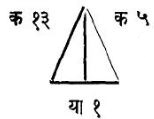
\includegraphics[scale=0.7]{Graphics/Capture18.JPG}
\end{minipage} 
\end{flushleft}
\vspace{-2mm}

\noindent च~। तथाहि भूमिः या १ अथ त्रिभुजे भुजयोर्योग\renewcommand{\thefootnote}{*}\footnote{लीलावत्यां क्षेत्रव्यवहारे श्लो ७१~। ८१~।} इत्यादिना आबाधे~। यथा क १३ क ५ अनयोर्योगः क १३ क ५ भुजयोरन्तरेणानेन क १३ क ५ं गुणनार्थं न्यासः $\begin{matrix}
\vspace{-1mm}
\mbox{क १३ क १३ क ५}\\
\vspace{-1.5mm}
\mbox{क ५ं क १३ क ५}
\vspace{1mm}
\end{matrix}$ गुणने जातानि करणीखण्डानि क १६९ क ६५ क ६ं५ क २ं५ अत्र मध्यमकरण्योर्धनर्णयोस्तुल्यत्वान्नाशः आद्यान्त्यकरण्योर्मूले रू १३ रू ५ं अनयोर्योगे जातं गुणनफलं रू ८ अयं भुवा हृतं\; $\begin{matrix}
\vspace{-1mm}
\mbox{रू ८}\\
\vspace{-1.5mm}
\mbox{या १}
\vspace{1mm}
\end{matrix}$\; लब्ध्या समछेदेन भूरूनयुता दलिता च जाते आबाधे $\begin{matrix}
\vspace{-1mm}
\mbox{याव १ रू ८ं}\\
\vspace{-1.5mm}
\mbox{या २ या २}
\vspace{1mm}
\end{matrix}$~। $\begin{matrix}
\vspace{-1mm}
\mbox{याव १ रू ८}\\
\vspace{-1.5mm}
\mbox{या २ या २}
\vspace{1mm}
\end{matrix}$~। लघोराबाधाया वर्गं $\begin{matrix}
\vspace{-1mm}
\mbox{या व व १}\\
\vspace{-1.5mm}
\mbox{याव ४}
\vspace{1mm}
\end{matrix}$ $\begin{matrix}
\vspace{-1mm}
\mbox{या व १ं६ रू ६४}\\
\vspace{-1.5mm}
\mbox{या व ४ ~याव ४}
\vspace{1mm}
\end{matrix}$ लघुभुजस्य क ५ वर्गात् रू ५ समछेदेनापास्य
$\begin{matrix}
\vspace{-1mm}
\mbox{या व व १}\\
\vspace{-1.5mm}
\mbox{याव ४}
\vspace{1mm}
\end{matrix}$ $\begin{matrix}
\vspace{-1mm}
\mbox{याव ३६ रू ६ं४}\\
\vspace{-1.5mm}
\mbox{याव ४ याव ४}
\vspace{1mm}
\end{matrix}$ जातो लम्बवर्गः~। एवं द्वितीयाबाधावर्गं $\begin{matrix}
\vspace{-1mm}
\mbox{या व व १}\\
\vspace{-1.5mm}
\mbox{याव ४}
\vspace{1mm}
\end{matrix}$ $\begin{matrix}
\vspace{-1mm}
\mbox{याव १६ रू ६४}\\
\vspace{-1.5mm}
\mbox{याव ४ याव ४}
\vspace{1mm}
\end{matrix}$ द्वितीयभुज\textendash \,क १३\textendash \,वर्गात् रू १६ समछेदेनापास्य वा जातो लम्बवर्गः स एव~। अथवा प्रकारान्तरेण लम्बगुणं भूम्यर्धं क्षेत्रफलं भवतीति व्यस्तविधिना भूम्यर्धेन या $\begin{matrix}
\vspace{-1.5mm}
\mbox{१}\\
\vspace{-1.5mm}
\mbox{२}
\vspace{1mm}
\end{matrix}$ क्षेत्रफलं ४ भक्ता जातो लम्बः $\begin{matrix}
\vspace{-1mm}
\mbox{रू ८}\\
\vspace{-1.5mm}
\mbox{या १}
\vspace{1mm}
\end{matrix}$ अस्य वर्गः $\begin{matrix}
\vspace{-1mm}
\mbox{रू ६४}\\
\vspace{-1.5mm}
\mbox{याव १}
\vspace{1mm}
\end{matrix}$ लम्बवर्गयोर्न्यासः $\begin{matrix}
\vspace{-1mm}
\mbox{या व व १}\\
\vspace{-1.5mm}
\mbox{याव ४}
\vspace{1mm}
\end{matrix}$ $\begin{matrix}
\vspace{-1mm}
\mbox{याव ३६ रू ६ं४}\\
\vspace{-1.5mm}
\mbox{याव ४ याव ४}
\vspace{1mm}
\end{matrix}$~।

\newpage%%%%%%%%%%%%%%%%%%%%%%%%%%%%%%%%%%%%%%%%%%%%%%%%%% 
\noindent $\begin{matrix}
\vspace{-1mm}
\mbox{या व व ०}\\
\vspace{-1.5mm}
\mbox{याव १}
\vspace{1mm}
\end{matrix}$ $\begin{matrix}
\vspace{-1mm}
\mbox{या व ० रू ६४}\\
\vspace{-1.5mm}
\mbox{याव १ याव १}
\vspace{1mm}
\end{matrix}$~। पक्षौ समछेदीकृत्य छेदगमे न्यासः $\begin{matrix}
\vspace{-1mm}
\mbox{या व व १ या व ३६}\\
\vspace{-1.5mm}
\mbox{या व व ० ~ याव ०}
\vspace{1mm}
\end{matrix}$ $\begin{matrix}
\vspace{-1mm}
\mbox{रू ६ं४}\\
\vspace{-1.5mm}
\mbox{रू २५६}
\vspace{1mm}
\end{matrix}$ समशोधने जातं याव $\begin{matrix}
\vspace{-1mm}
\mbox{रू ३२ं०}\\
\vspace{-1.5mm}
\mbox{या व व १ या व ३ं६} 
\vspace{1mm}
\end{matrix}$ अथाव्यक्तवर्गादि यदा शेषमित्यादि-वक्ष्यमाणमध्यमाहरणविधिना पक्षयोरष्टादशवर्गं ३२४ प्रक्षिप्य गृहीते मूले $\begin{matrix}
\vspace{-1mm}
\mbox{रू २ ~~~~~~}\\
\vspace{-1.5mm}
\mbox{याव १ रू १ं८} 
\vspace{1mm}
\end{matrix}$~। $\begin{matrix}
\vspace{-1mm}
\mbox{रू २ं ~~~~~~}\\
\vspace{-1.5mm}
\mbox{याव १ रू १ं८} 
\vspace{1mm}
\end{matrix}$~। अव्यक्तपक्षर्णगरूपतोल्पमित्यादिना जातं द्विविधं यावत्तावद्वर्गमानं २०~। १६~। अत्राद्यमनुपपन्नत्वान्न ग्राह्यम्~। अनुपपत्तावुपपत्तिं तु मध्यमाहरणविवरणे वक्ष्यामः~। यावत्तावद्वर्गमानस्य १६ पदं ४ जातं यावत्तावन्मानम्~॥\\

\vspace{-3mm}
 इयमेव भूः ४~। अथ पूर्वसिद्धलम्बवर्गं $\begin{matrix}
\vspace{-1mm}
\mbox{या व व १}\\
\vspace{-1.5mm}
\mbox{याव ४}
\vspace{1mm}
\end{matrix}$ $\begin{matrix}
\vspace{-1mm}
\mbox{याव ३६ रू ६ं४}\\
\vspace{-1.5mm}
\mbox{याव ४ याव ४}
\vspace{1mm}
 \end{matrix}$ भूम्यर्धं वर्गेण~। याव $\begin{matrix}
\vspace{-1.5mm}
\mbox{१}\\
\vspace{-1.5mm}
\mbox{४}
\vspace{1mm}
\end{matrix}$~। सङ्गुण्य जातः क्षेत्रफलवर्गः~। $\begin{matrix}
\vspace{-1mm}
\mbox{या व व १}\\
\vspace{-1.5mm}
\mbox{~~~~~ १६}
\vspace{1mm}
\end{matrix}$ याव $\begin{matrix}
\vspace{-1mm}
\mbox{३६}\\
\vspace{-1.5mm}
\mbox{१६}
\vspace{1mm}
 \end{matrix}$ रू $\begin{matrix}
\vspace{-1.5mm}
 \mbox{६ं४}\\
\vspace{-1.5mm}
 \mbox{१६}
\vspace{1mm}
 \end{matrix}$ अयं क्षेत्रफलस्यास्य ४ वर्गेण सम इति समशोधनार्थं न्यासः
$\begin{matrix}
\vspace{-1mm}
\mbox{या व व १ं}\\
\vspace{-1.5mm}
\mbox{या व व ०}
\vspace{1mm}
\end{matrix}$ $\begin{matrix}
\vspace{-1mm}
\mbox{या व ३६ रू ६ं४}\\
\vspace{-1.5mm}
\mbox{याव ० रू २५६}
\vspace{1mm}
 \end{matrix}$ पक्षौ समच्छेदीकृत्य छेदगमे प्राग्वल्लब्धं 
यावत्तावन्मानं ४ तदेव भूमियावत्तावत्कल्पने क्रिया प्रसरति~। अत 
आचार्येणाव्यक्तकल्पनानिरपेक्षमेव यथोदाहरणसिद्धिर्भवेत्तथा स्वेच्छया एको भुजो~क~१३
\vspace{-8mm}

\begin{flushleft}
\begin{minipage}[c]{0.7\textwidth}
भूमिः कल्पिता~। फले विशेषाभावात्~। दर्शनं क्षेत्रफलं रू ४ लम्बगुणं भूम्यर्धं क्षेत्रफलं भवतीति क्षेत्रफलं भूम्यर्धभक्तं लम्बः स्यात्~। तत्र यद्यपि द्वाभ्यां भागेऽर्धं भवतीति भूमेरर्धार्थं द्वाभ्यां भाग उचितस्तथापि वर्गेण वर्गं भजेदित्युक्तत्वात्प्रकृते वर्गरूपाया भूमेरर्धार्थं
\end{minipage} 
\hfill
\begin{minipage}{0.25\textwidth} 
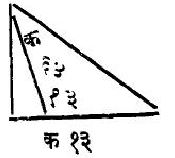
\includegraphics[scale=0.65]{Graphics/Capture19.JPG}
\end{minipage} 
\end{flushleft}

\newpage %%%%%%%%%%%%%%%%%%%%%%%%%%%%%%%%%%%%१७३ 
\noindent चतुर्भिरेव भाग उचितः एवं जातं भूम्यर्धं क $\begin{matrix}
\vspace{-1.5mm}
\mbox{१३}\\
\vspace{-1.5mm}
\mbox{४}
\vspace{1mm}
\end{matrix}$ उक्तवत्क्षेत्रफलमपि वर्गीकृतं क १६~। क्षेत्रफलेऽस्मिन् क १६ भूम्यर्धेनानेन क $\begin{matrix}
\vspace{-1.5mm}
\mbox{१३}\\
\vspace{-1.5mm}
\mbox{४}
\vspace{1mm}
\end{matrix}$ भक्ते जातो लम्बः क $\begin{matrix}
\vspace{-1.5mm}
\mbox{६४}\\
\vspace{-1.5mm}
\mbox{१३}
\vspace{1mm}
\end{matrix}$~। अस्य कोटिरूपस्य वर्गं $\begin{matrix}
\vspace{-1.5mm}
\mbox{६४}\\
\vspace{-1.5mm}
\mbox{१३}
\vspace{1mm}
\end{matrix}$ ज्ञातभुजस्य कर्णरूपस्य क ५ वर्गात् रू ५ अपास्य रू
$\begin{matrix}
\vspace{-1.5mm}
\mbox{१}\\
\vspace{-1.5mm}
\mbox{१३}
\vspace{1mm}
\end{matrix}$~। मूलं क $\begin{matrix}
\vspace{-1.5mm}
\mbox{१}\\
\vspace{-1.5mm}
\mbox{१३}
\vspace{1mm}
\end{matrix}$~। जाता लघुराबाधा~। यथा करण्या वर्गे तत्तुल्यानि रूपाणि भवन्ति तथा रूपाणां मूले रूपतुल्या करणीं भवितुमर्हति~। यतो यस्य राशेर्यो वर्गस्तस्य वर्गस्य स राशिर्मूलमिति~। अथाबाधां क $\begin{matrix}
\vspace{-1.5mm}
\mbox{१}\\
\vspace{-1.5mm}
\mbox{१३}
\vspace{1mm}
\end{matrix}$ भूमेः क १३ अपास्य योगं करण्योरित्यादिना 
लघ्वा हृतायास्त्वित्यादिना वा जातान्याबाधा~। क $\begin{matrix}
\vspace{-1.5mm}
\mbox{१४४}\\
\vspace{-1.5mm}
\mbox{१३}
\vspace{1mm}
\end{matrix}$~। इयमाबाधा भुजः लम्बः कोटिः~। अज्ञातभुजः कर्णः~। अत्र भुजकोटयोर्ज्ञाने तत्कृत्योर्योगपदं कर्ण इति कर्णः सुलभः~। द्वितीयाबाधायाः~। क 
$\begin{matrix}
\vspace{-1.5mm}
\mbox{१४४}\\
\vspace{-1.5mm}
\mbox{१३}
\vspace{1mm}
\end{matrix}$~। वर्गः~। रू $\begin{matrix}
\vspace{-1.5mm}
\mbox{१४४}\\
\vspace{-1.5mm}
\mbox{१३}
\vspace{1mm}
\end{matrix}$ लम्बस्य~। क $\begin{matrix}
\vspace{-1.5mm}
\mbox{६४}\\
\vspace{-1.5mm}
\mbox{१४}
\vspace{1mm}
\end{matrix}$~। वर्गेण~। रू $\begin{matrix}
\vspace{-1.5mm}
\mbox{६४}\\
\vspace{-1.5mm}
\mbox{१३}
\vspace{1mm}
\end{matrix}$~। युतः १६~। अस्य पदं रू ४ ज्ञातोऽज्ञातभुजः प्रष्टाया भूमिपृष्टा सैवाचार्येण भुजत्वेण कल्पिता~। तस्मादत्र यो 
\begin{flushleft}
\begin{minipage}[c]{0.7\textwidth}
भुजोऽवगतः रू ४ इयमेव सा भूः~। एवमन्यं भुजं क ५ भूमिं प्रकल्प्य न्यासः क १३ अत्रापि पूर्ववत्फलालम्बः~। क $\begin{matrix}
\vspace{-1mm}
 \mbox{६४}\\
\vspace{-1.5mm}
 \mbox{५}
\vspace{1mm}
 \end{matrix}$ लम्बवर्गं रू $\begin{matrix}
\vspace{-1.5mm}
 \mbox{६४}\\
\vspace{-1.5mm}
 \mbox{५}
\vspace{1mm}
 \end{matrix}$ भुजवर्गात् रू १३ अपास्य रू $\begin{matrix}
\vspace{-1.5mm}
 \mbox{१}\\
\vspace{-1.5mm}
 \mbox{५}
\vspace{1mm}
 \end{matrix}$ मूलं क $\begin{matrix}
\vspace{-1.5mm}
 \mbox{१}\\
\vspace{-1.5mm}
 \mbox{५}
\vspace{1mm}
 \end{matrix}$ जाताबाधा~। इमं
\end{minipage} 
\hfill
\begin{minipage}{0.25\textwidth} 
\hspace{4mm} 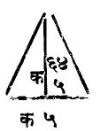
\includegraphics[scale=0.8]{Graphics/Capture20.JPG}
\end{minipage} 
\end{flushleft}

\newpage%%%%%%%%%%%%%%%%%%%%%%%%%%%%%%%%%%%%%%%%%%%%%%%%%% 
\noindent योगं करण्योरित्यादिना भूमेः क ५ अपास्य जातान्या क 
$\begin{matrix}
\vspace{-1.5mm}
\mbox{१६}\\
\vspace{-1.5mm}
\mbox{५}
\vspace{1mm}
\end{matrix}$~। अस्या वर्गात् रू $\begin{matrix}
\vspace{-1.5mm}
\mbox{१६}\\
\vspace{-1.5mm}
\mbox{५}
\vspace{1mm}
\end{matrix}$ १६५ लम्बवर्गेण रू $\begin{matrix}
\vspace{-1.5mm}
\mbox{६४}\\
\vspace{-1.5mm}
\mbox{५}
\vspace{1mm}
\end{matrix}$ युतात् १६ मूलं ज्ञातोऽज्ञातभुजः ४ 
एवमन्यत्रापि सुधीभिरूह्यम्~। अथान्यदुदाहरणमार्ययाह\textendash
\begin{quote}
    \ex
     दशपञ्चकरण्यन्तरमेको बाहुः परश्च षट्करणी~। \\
 भूरष्टादशकरणीरूपोना लम्बमाचक्ष्व~॥~५२~॥~
\end{quote}

\begin{flushleft}
\begin{minipage}[c]{0.55\textwidth}
\hspace{4mm} स्पष्टोऽर्थः~। अत्राबाधाज्ञाने लम्बज्ञानमिति लघुराबाधा कल्पिता या १~। एतदूना भूरन्याबाधेति~। तथा न्यासः अत्राबाधे भुजौ~। भुजौ तु कर्णौ कोटिरुभयत्र लम्ब एवेति~। स्वाबाधावर्गं स्वभुजवर्गादपास्य लम्बवर्गौ भवतः~। तत्र लघोः
\end{minipage} 
\hfill
\begin{minipage}{0.4\textwidth} 
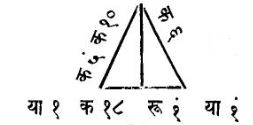
\includegraphics[scale=0.7]{Graphics/Capture21.JPG}
\end{minipage} 
\end{flushleft}
\vspace{-3mm}

\noindent आबाधाया वर्गः याव १ लघुभुजस्यास्य क ५ं क १० स्थाप्योऽन्त्यवर्गश्चतुर्गुणान्त्यनिघ्ना इत्यादिना~। क २५ क २०ं० 
क १०० आद्यान्त्यकरण्योर्योगे कृते क २२५ मूले च गृहीते रू १५ जातो 
लघुभुजवर्गः रू १५ क २०ं०~। अयमाबाधावर्गोनः सन् जातो लम्बवर्गः 
याव १ं रू १५ क २०ं०~। एवं द्वितीयाबाधायाः या १ं रू १ं क १८ 
अत्र स्थाप्योऽन्त्यवर्ग इत्यादिना यथासम्भवं द्विगुणान्त्यनिघ्नाश्चतुर्गुणान्त्यनिघ्नाश्चेति 
कृते जातो वर्गः~। याव १ या २ याक ७ं२ रू १ क ७ं२ क ३२४~। 
अन्त्यकरण्या मूलं रू १८ रूपेण संयोज्य परखण्डानां भिन्नजातित्वात् 
पृथक्स्थितौ च जातः याव १ या २ याक ७ं२ रू १९ क ७ं२~। 
एनमाबाधावर्गस्वभुजस्यास्य क ६ वर्गादस्मात् रू ६ विशोध्य वा जातो 
लम्बवर्गः याव १ं या २ं याक ७२ रू १ं३ क ७२~। लम्बवर्गो समाविति 
समशोधनार्थे न्यासः $\begin{matrix}
\vspace{-1mm}
\mbox{{याव १ या ० या का ० रू १५ क २०ं०}}\\
\vspace{-1.5mm}
\mbox{{याव १ं या २ं याक ७२ रू १ं३ क ७२}}
\vspace{1mm}
\end{matrix}$~। 

\newpage %%%%%%%%%%%%%%%%%%%%%%%%%%%%%%%%%%%%१७५ 

\noindent आत्राद्यपक्षादव्यक्तमात्रे शोधिते इतरस्माच्च व्यक्तमात्रे शोधिते
$\begin{matrix}
\vspace{-1mm}
\mbox{या २~}\\
\vspace{-1.5mm}
\mbox{रू २ं८}
\vspace{1mm}
\end{matrix}$ $\begin{matrix}
\vspace{-1mm}
\mbox{~~~~ याक ७ं२}\\
\vspace{-1.5mm}
\mbox{क २०० क ७२}
\vspace{1mm}
\end{matrix}$~। योगं करण्योरित्यदिना करण्योर्योगे च कृते जाते शेषे 
$\begin{matrix}
\vspace{-1mm}
\mbox{या २ं}\\
\vspace{-1.5mm}
\mbox{रू २८}
\vspace{1mm}
\end{matrix}$ $\begin{matrix}
\vspace{-1mm}
\mbox{याक ७२}\\
\vspace{-1.5mm}
\mbox{क ५१ं२}
\vspace{1mm}
\end{matrix}$~। अथाव्यक्तशेषेण व्यक्तशेषस्य भागार्थं न्यासः~। रू २८ क ५१ं२ अत्राव्यक्तशेषेण व्यक्तशेषं कथं भाज्यमित्याह~। अत्र या २ं याक ७२ याकारस्य प्रयोजनाभावादपगमे कृते समभाज्यभाजकाविति $\begin{matrix}
\vspace{-1mm}
\mbox{रू २ं८ क ५१२}\\
\vspace{-1.5mm}
\mbox{रू २ ~क ७ं२}
\vspace{1mm}
\end{matrix}$~। \\

\vspace{-1mm}
 वस्तुतस्तु अव्यक्तशेषतुल्येनाव्यक्तेन यादि व्यक्तशेषतुल्यं व्यक्तं 
लभ्यते तदा एकेनाव्यक्तेन किमिति त्रैराशिकेन~। या २ याक ७ं२~। 
रू २ं८ क ५१२~। या १~। अव्यक्तस्य व्यक्तमानं \,भवति \,इति \,इच्छाप्रमाणयोर्यावत्तावतापवर्ते \,भवतीष्टो \,हरः \,रू २ \,क ७ं२~। अन्यथान्यत्रापि अव्यक्तशेषेण रूपशेषे भक्ते रूपात्मकं फलं कथं स्यात्~। आचार्यैस्त्वन्यत्र याकारस्यानपगमेऽपि अज्ञानां गणितसिद्धिर्भवतीति तत्र याकारापगमो नोक्तः प्रकृते तु याकारानपगमे धनर्णताव्यत्ययमीप्सितायाश्छेदे करण्या इत्यादिना भाज्यभाजयकयोर्गुणने भूयाननर्थः स्यादिति याकारापगम उक्तः~॥~\\

\vspace{-3mm}
 अथ द्विसप्ततिमिताया भाजककरण्या धनत्वं प्रकल्प्य धनत्वं प्रकल्प्य 
तादृक्छिदा~। क ४ क ७२ भाज्यभाजकयोर्गुणनार्थं न्यासः~। $\begin{matrix}
\vspace{-1mm}
\mbox{क ४}\\
\vspace{-1.5mm}
\mbox{क ७२}
\vspace{1mm}
\end{matrix}$~। $\begin{matrix}
\vspace{-1mm}
\mbox{क ७८ं४}\\
\vspace{-1.5mm}
\mbox{क ७८ं४}
\vspace{1mm}
\end{matrix}$~। $\begin{matrix}
\vspace{-1mm}
\mbox{क ५१२}\\
\vspace{-1.5mm}
\mbox{क ५१२}
\vspace{1mm}
\end{matrix}$~। $\begin{matrix}
\vspace{-1mm}
\mbox{क ४}\\
\vspace{-1.5mm}
\mbox{क ७२}
\vspace{1mm}
\end{matrix}$~। $\begin{matrix}
\vspace{-1mm}
\mbox{क ४}\\
\vspace{-1.5mm}
\mbox{क ४}
\vspace{1mm}
\end{matrix}$~। $\begin{matrix}
\vspace{-1mm}
\mbox{क ७ं२}\\
\vspace{-1.5mm}
\mbox{क ७ं२}
\vspace{1mm}
\end{matrix}$~। भाज्ये गुणिते जातानि खण्डानि क ३१ं३६ क २०४८ क ५६४ं४८ क ३६८६४~। अत्राद्यान्त्ययोः द्वितीयतृतीययोश्च करण्योर्लघ्वाहृतायास्तु
पदमित्यादिनान्तरे कृते
 \newpage%%%%%%%%%%%%%%%%%%%%%%%%%%%%%%%%%%%%%%%%%%%%%%%%%% 

\noindent जाते भाज्यकरण्यौ क १८४९६ क ३६९ं९२~॥ एवं भाजके करणीखण्डानि क १६ क २८ं८ क २८८ क ५१ं८४~। अत्र द्वितीयतृतीयकरण्योरन्तरे नाशः~। आद्यान्त्ययोरन्तरे कृते जाता भाजककरणी क ४६ं२४~। अनया भाज्ये हते लब्धं यावत्तावन्मानं क ४ं क ८~। प्रथमकरण्या मूले गृहीते जातं रू २ं क ८~। इयमेव लघुराबाधा~। एतदूना भूः रू १ं क १८ 
योगं करण्योरित्यन्तरे कृते जाता द्वितीयाबाधा~। रू १ क २~॥~अथ 
प्रथमलम्बवर्गस्योत्थापनार्थं न्यासः या व १ं रू १५ क २०ं०~। अत्राद्यमेव 
खण्डमव्यक्तं स च यावद्वर्गोऽस्ति~। अतो यावत्तावन्मानस्यास्य क ४ं क ८
वर्गो रू १२ क १२८ जातं यावत्तावद्वर्गमानम्~। यावद्वर्गस्य ऋणगतत्वादिदं रू १२ क १२ं८ उत्तरखण्डद्वयादस्मात् रू १५ क २०ं० विशोध्य
जातो लम्बवर्गः रू ३ क ८ं~। एवं द्वितीयस्य लम्बवर्गस्योत्थापनार्थं न्यासः 
यव १ं या २ं या क ७२ रू १ं३ क ७२~। अत्राद्य खण्डत्रयमव्यक्तम्~। 
तत्र प्रथमखण्डस्य पूर्ववन्मानं रू १२ क १२ं८~। द्वितीयखण्डे
यावत्तावद्दयमस्तीति यावत्तावन्मानं रू २ं क ८ द्वाभ्यां सङ्गुण्य वर्गेण वर्गं गुणयेदिति 
करणीचतुर्भिः सङ्गुण्य जातं द्वितीयखण्डमानं रू ४ं क ३२~॥~\\

\vspace{-3mm}
 अथ तृतीयस्य~। यद्येकेन यावत्तावता व्यक्तमानमिदं क ४ं क ८ 
तदाभीष्टेनानेन या क ७२ किमिति त्रैराशिकार्थं न्यासः या १~। क ४ं क ८~। 
या क ७२~। अत्र प्रमाणेच्छयोः प्रमाणेनापवर्ते कृतेऽपवर्तितेच्छया क ७२
फले गुणिते जातं तृतीयखण्डमानम्~। क २८ं८ क ५७६~। द्वितीयकरण्या 
मूले गृहीते जातं रू २४ क २८ं८~। एवं जातान्यव्यक्तखण्डत्रयस्य 
व्यक्तमानानि रू १२ क १२ं८ रू ४ं क ३२ रू २४ क २८ं८~। अत्र 
लम्बवर्गे आद्ययोरव्यक्तखण्डयोर्ऋणत्वेन शोध्यत्वात्तदुथ्यव्यक्तयोरपि
शोध्य-त्वेन संशोध्यमानं स्वमृणत्वमेतीत्यादिना जातं रू १ं२ क १२८ रू ४ क ३ं२ 
रू २४ क २८ं८ रू १ं३ क ७२~। अत्र रूपाणां यथोक्तयोगे कृते जातं रू ३~। आद्ययोः करण्योः क १२८ क ३२ अन्तरे जातं क ३२~। अस्यास्तृतीयकरण्या सह २८८ अन्तरे जातं क १२८~। अस्याः
\newpage %%%%%%%%%%%%%%%%%%%%%%%%%%%%%%%%%%%%१७७ 
\noindent पुनरन्त्यया क ७२ अन्तरे जातम् क ८ं~। अथवा ऋणकरण्योरनयोः 
क ३२ क २८८ धनकरण्योरनयोश्च क १२८ क ७२ योगे जातं 
करणीद्वयम् क ५१ं२ क ३९२~। अनयोरन्तरे जाता सैव करणी क ८ं~। 
एवं जातो लम्बवर्गः स एव रू ३ क ८ं~। अथवा आबाधा क ४ं क ८ 
वर्गं रू १२ क १२ं८ स्वभुजकय\textendash \,क ५ं क १०\textendash \,वर्गात् रू १५ क २०ं० 
उक्तवदपास्य जातो लम्बवर्गः स एव रू ३ क ८ं एवं द्वितीयाबाधा क १ 
क २ वर्गं रू ३ क ८ स्वभुज\textendash \,क ६\textendash \,वर्गात् रू ६ अपास्य जातो लम्बवर्गः स एव रू ३ क ८ं~। अथास्य पदं तत्र ऋणात्मिका चेत्करणीकृतौ स्याद्धनात्मिकां तां परिकल्प्येति कृते रूपकृते ९ करणीतुल्यानि रूपाणि ८ अपास्य शेषस्य १ पदेन १ रूपाणि ३ युतोनितानि ४।२ अर्धे २।१ ऋणात्मिकैका सुधियावगम्येति अल्पकरण्या ऋणत्वे कृते पदे च गृहीते 
जातो लम्बः रू १ं क २~। इदमुदाहरणं व्यक्तमार्गेणापि सिध्यन्ति~। 
तद्यथा त्रिभुजे भुजयोर्योग इत्यादिना~। भुजयोरनयोः क ५ं क १० 
क ६ योगः क ५ं क १० क ६ लघुभुजं क ५ं क १० महतो 
भुजात् क ६ अपास्य जातं भुजयोरन्तरम्~। क ५ क १ं० क ६ 
अन्तरेण योगस्य गुणनार्थं न्यासः $\begin{matrix}
\vspace{-1mm}
\mbox{{क ५ ~क ५ं क १० क ६}}\\
\vspace{-1.5mm}
\mbox{{क १ं० क ५ं क १० क ६}}\\
\vspace{-1.5mm}
\mbox{{क ६ ~क ५ं क १० क ६}}
\vspace{1mm}
\end{matrix}$ गुणिते जातं खण्डनवकम् क २ं५ क ५० क ३० क ५० क १०ं० क ६ं० क ३ं० क ६० क ३६~। अत्र त्रिंशन्मितकरण्योः षष्टिमितकरण्योश्च धनर्णत्वान्नाशे पञ्चाशतकरण्योर्योगे च कृते क २०० शेषकरणीमूलानां ५ं~। १ं०~। ६~। योगे च कृते जातं गुणनफलं रू ९ं क २००~। इदं भूभ्यानया रू १ं क १८ 
भाज्यम्~॥~\\

\vspace{-3mm}
 अत्र वर्गेण वर्गं भजेदित्युक्तेः क्षयो भवेच्च क्षयरूपवर्ग इति 
रूपवर्गे कृते जातौ भाज्यभाजकौ $\begin{matrix}
\vspace{-1mm}
\mbox{{क ८ं१ क २००}}\\
\vspace{-1.5mm}
\mbox{{क १ं ~क १८}}
\vspace{1mm}
\end{matrix}$~। अथ भाजकस्यैकी- 

\newpage%%%%%%%%%%%%%%%%%%%%%%%%%%%%%%%%%%%%%%%%%%%%%%%%%% 
\noindent करणार्थं धनर्णताव्यत्ययमीप्सिताया इत्यादिना भाजकरण्यां १ धनत्वं 
प्रकल्प्य तादृक्छिदा क १ क १८ भाज्यभाजकयोर्गुणनार्थं न्यासः $\begin{matrix}
\vspace{-2mm}
\mbox{{क १~}}\\
\vspace{-1.5mm}
\mbox{{क १८}}
\vspace{1mm}
\end{matrix}$ $\begin{matrix}
\vspace{-2mm}
\mbox{{क ८ं१}}\\
\vspace{-1.5mm}
\mbox{{क ८ं१}}
\vspace{1mm}
\end{matrix}$ $\begin{matrix}
\vspace{-2mm}
\mbox{{क २००}}\\
\vspace{-1.5mm}
\mbox{{क २००}}
\vspace{1mm}
\end{matrix}$~। $\begin{matrix}
\vspace{-2mm}
\mbox{{क १~}}\\
\vspace{-1.5mm}
\mbox{{क १८}}
\vspace{1mm}
\end{matrix}$ $\begin{matrix}
\vspace{-2mm}
\mbox{{क १ं}}\\
\vspace{-1.5mm}
\mbox{{क १ं}}
\vspace{1mm}
\end{matrix}$ $\begin{matrix}
\vspace{-2mm}
\mbox{{क १८}}\\
\vspace{-1.5mm}
\mbox{{क १८}}
\vspace{1mm}
\end{matrix}$~। भाज्ये गुणिते जातानि करणीखण्डानि क ८ं१ क २०० क १४ं५८ क ३६००~। आद्यन्तकरण्योर्मध्यमकरण्योश्चान्तरे जातो भाज्यः क २६०१ क ५७ं८~। भाजके गुणिते जातं क १ं क १८ क १ं८ क ३२४~। मध्यमकरण्योर्नाशे आद्यान्त्यकरण्योरन्तरे कृते जाता भाजके एकैव करणी क २८९~। अनया भाज्ये भक्ते लब्धिः क ९ क २ं प्रथमकरण्याः पदे जाता लब्धिः रू ३ क २ं 
अनया भूरेषा रू १ं क १८ यथावदूना रू ४ं क ३२ युता रू २ क ८ 
यथावदर्धिता~। रू २ं क ८~। रू १ क २~। जाते आबाधे~। \\

 \vspace{-3mm}
 आभ्यां पूर्ववल्लम्बः रू १ क २~। 

\begin{flushleft}
\begin{minipage}[c]{0.65\textwidth}
\hspace{4mm} आसन्नमूलग्रहणेन जाताः क्षेत्रभुजाद्याः दर्शनम् अत्र दशपञ्चकरण्योरासन्नमूले ३।१०॥२।१४~॥ अनयोरन्तरमेको भुजः ०।५६ एवं सर्वत्र द्रष्टव्यम्~। अत्रापि प्रतीत्यर्थं गणितं लिख्यते~। भुजयोः $\begin{matrix}
\vspace{-1.5mm}
\mbox{०}\\
\vspace{-1.5mm}
\mbox{५६}
\vspace{1mm}
\end{matrix}$~। $\begin{matrix}
\vspace{-1.5mm}
\mbox{२}\\
\vspace{-1.5mm}
\mbox{२७}
\vspace{1mm}
\end{matrix}$~। योगः $\begin{matrix}
\vspace{-1.5mm}
\mbox{३}\\
\vspace{-1.5mm}
\mbox{२३}
\vspace{1mm}
\end{matrix}$ भुजयोः अन्तरेण $\begin{matrix}
\vspace{-1.5mm}
 \mbox{१}\\
\vspace{-1.5mm}
 \mbox{३१}
\vspace{1mm}
 \end{matrix}$ गुणितः $\begin{matrix}
\vspace{-1.5mm}
 \mbox{५}\\
\vspace{-1.5mm}
 \mbox{८}
\vspace{1mm}
 \end{matrix}$ भुवा $\begin{matrix}
\vspace{-1.5mm}
 \mbox{३}\\
\vspace{-1.5mm}
 \mbox{१५}
\vspace{1mm}
 \end{matrix}$ हृतो लब्धिः $\begin{matrix}
\vspace{-1.5mm}
 \mbox{१}\\
\vspace{-1.5mm}
 \mbox{३५}
\vspace{1mm}
 \end{matrix}$ अनया
\end{minipage} 
\hfill
\begin{minipage}{0.3\textwidth} 
\vspace{-8mm}

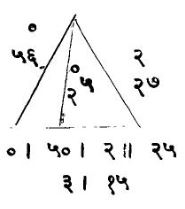
\includegraphics[scale=0.7]{Graphics/Capture22.JPG}
\end{minipage} 
\end{flushleft}
\vspace{-6mm}

\noindent द्विष्टा भूरूनयुता $\begin{matrix}
\vspace{-1.5mm}
 \mbox{१}\\
\vspace{-1.5mm}
 \mbox{४०}
\vspace{1mm}
 \end{matrix}$ $\begin{matrix}
\vspace{-1.5mm}
 \mbox{४}\\
\vspace{-1.5mm}
  \mbox{५०}
\vspace{1mm}
 \end{matrix}$ दलिता जाते आबाधे $\begin{matrix}
\vspace{-1.5mm}
 \mbox{०}\\
\vspace{-1.5mm}
 \mbox{५०}
\vspace{1mm}
 \end{matrix}$ $\begin{matrix}
\vspace{-1.5mm}
 \mbox{२}\\
\vspace{-1.5mm}
 \mbox{२५}
\vspace{1mm}
 \end{matrix}$~। अथाबाधा\textendash \,$\begin{matrix}
\vspace{-1.5mm}
 \mbox{०}\\
\vspace{-1.5mm}
 \mbox{५०}
\vspace{1mm}
 \end{matrix}$\textendash \,वर्गं $\begin{matrix}
\vspace{-1.5mm}
 \mbox{०}\\
\vspace{-1.5mm}
 \mbox{४२}
\vspace{1mm}
 \end{matrix}$ स्वभुज\textendash \,$\begin{matrix}
\vspace{-1.5mm}
 \mbox{०}\\
\vspace{-1.5mm}
 \mbox{५६}
\vspace{1mm}
 \end{matrix}$\textendash \,वर्गात् $\begin{matrix}
\vspace{-1.5mm}
 \mbox{०}\\
\vspace{-1.5mm}
 \mbox{५२}
\vspace{1mm}
 \end{matrix}$ अपास्य शेषस्य $\begin{matrix}
\vspace{-1.5mm}
 \mbox{०}\\
\vspace{-1.5mm}
 \mbox{१०}
\vspace{1mm}
 \end{matrix}$ मूलं $\begin{matrix}
\vspace{-1.5mm}
 \mbox{०}\\
\vspace{-1.5mm}
 \mbox{२५}
\vspace{1mm}
 \end{matrix}$ जातो लम्बः एवं द्वितीयाबाधा\textendash \,$\begin{matrix}
\vspace{-1.5mm}
 \mbox{२}\\
\vspace{-1.5mm}
 \mbox{२५}
\vspace{1mm}
 \end{matrix}$\textendash \,वर्गं $\begin{matrix}
\vspace{-1.5mm}
 \mbox{५}\\
\vspace{-1.5mm}
 \mbox{५०}
\vspace{1mm}
 \end{matrix}$ स्वभुज\textendash \,$\begin{matrix}
\vspace{-1.5mm}
 \mbox{२}\\
\vspace{-1.5mm}
 \mbox{२७}
\vspace{1mm}
 \end{matrix}$\textendash 
\newpage 
%%%%%%%%%%%%%%%%%%%%%%%%%%%%%%%%%%%%
\noindent वर्गात् ६ अपास्य शेषस्य $\begin{matrix}
\vspace{-1.5mm}
\mbox{०}\\
\vspace{-1.5mm}
\mbox{१०}
\vspace{1mm}
\end{matrix}$ मूलं जातो लम्बः स एव $\begin{matrix}
\vspace{-1.5mm}
\mbox{०}\\
\vspace{-1.5mm}
\mbox{२५}
\vspace{1mm}
\end{matrix}$ एवमन्यत्रापि सुधीभिरूह्मम्~। \\

\vspace{-2mm}
 अथ पक्षयोः समशोधनानन्तरं अव्यक्तवर्गधनादिकेऽपि शेषे यथासम्भवम् अपवर्तेन मध्यमाहरणं विनैवोदाहरणसिद्धिरस्तीति प्रदर्शयितुमुदाहरणषट्कमाह~। \\

\vspace{-3mm}
 तत्रोदाहरणद्वयमनुष्टभाह\textendash 
\begin{quote}
    \ex
     असमानसमच्छेदान् राशींस्तांश्चतुरो वद~। \\
 यदैक्यं यद्धनैक्यं वा येषां वर्गैक्यसम्मितम्~॥~५३~॥~
\end{quote}

असमानाश्च ते समच्छेदाश्च तान्~। यदैक्यं येषां वर्गैक्यसम्मितमित्येकं 
यद्धनैक्यं येषां वर्गैक्यसम्मितमिति द्वितीयमित्युदाहरणद्वयम्~। असमानसमप्रज्ञेति 
पाठे तु हे असमप्रज्ञा निरुपमबुद्धे; असमांस्तांश्चतुरो राशीन्वदेति
योजनीयम्~। प्रथमपाठस्त्वसाधुरिति प्रतिभाति~। नहि समछेदत्वपुरस्कारेणोदाहरणमिह साध्येते किन्तु समछेदत्वं सम्पाता यातम्~। असमानिति त्वपेक्षितमेव~। अन्यथा रूपमितैश्चतुर्भिरुदाहरणसिद्धेः~। \\

\vspace{-3mm}
 अत्र राशीनामसमत्वेनोद्देशात् कल्पिताच्च तुल्यराशयः या १ या २ 
या ३ या ४ उदाहरणद्वयस्यापि गणितं त्वाकर एव स्फुटम्~। \\

\vspace{-3mm}
 अन्यदुदाहरणद्वयमनुष्टभाह\textendash 
\begin{quote}
    \ex
    त्र्यस्रक्षेत्रस्य यस्य स्यात्फलं कर्णेन सम्मितम्~। \\
 दोःकोटिश्रुतिघातेन समं यस्य च तद्वद~॥~५४~॥~
\end{quote}
 
स्पष्टोऽर्थः~। अत्र दोःकोटिकर्णानामव्यक्तकल्पने विशेषोऽस्ति~। जात्यत्र्यस्रेऽनियतानां तेषां बाधितत्वात्~। अत इष्टजात्यस्य भुजकोटिकर्णैः पृथग्गुणितं यावत्तावत्तेषां मानानि प्रकल्प्योदाहरणद्वयमपि साध्यम्~। आकर
एव स्पष्टमन्यत्~। अन्यदुदाहरणमनुष्टभाह\textendash
 \newpage%%%%%%%%%%%%%%%%%%%%%%%%%%%%%%%%%%%%%%%%%%%%%%%%%% 
 
\begin{quote}
    \ex
    युतौ वर्गान्तरे वर्गो ययोर्घाते घनो भवेत्~। \\
 तौ राशी शीघ्रमाचक्ष्व दक्षोऽसि गणिते यदि~॥~५५~॥~
\end{quote}
 
ययोः राश्योर्युतावन्तरे च वर्गो भवेत् घाते तु घनो भवेत् तौ राशी शीघ्रं वद~। \\

\vspace{-3mm}
 अत्र क्रियासङ्कोचार्थं तथा राशी कल्प्यौ यथा युतावन्तरे च वर्गः 
स्यात्~। तथा कल्पितौ~। याव ४ याव ५ अनयोर्घातः याव व २०~। 
एष घन इति इष्टयावत्तावद्दशकस्य घनेन याघ १००० समीकरणे पक्षौ 
यावत्तावद्धनेनापवर्त्य प्राग्वज्जातौ राशी १००००~। १२५००~। \\

\vspace{-3mm}
 अथान्यदुदाहरणमनुष्टभाह\textendash 
\begin{quote}
    \ex
     घनैक्यं जायते वर्गो वर्गैक्यं च ययोर्घनः~। \\
 तौ चेद्वेत्सि तदाहं त्वां मन्ये बीजविदां वरम्~॥~५६~॥
\end{quote}

स्पष्टोऽर्थः~। अत्र यथैक आलापः स्वतः सम्भवति तथा राशी कल्पितौ~। याव १ याव २ अनयोर्घनयोगः यावघ ९~। एष स्वयमेव वर्गो जातः 
यतोऽस्य वर्गमूलमिदम्~। याद्य ३~। अस्मिन्नर्थे आकर एवाक्षिप्य समाहितम्~। 
अयमर्थः यावद्वर्गघनौ राशिः षट् घातात्मकोऽस्ति~। सद्विघातस्य समत्रिघातो 
भवतीति यथा द्विघातस्य घनस्तथा त्रिघातस्य समद्विघातो भवतीति 
त्रिघातस्य वर्गोऽपि भवितुं युक्त एवेति~। अथ तयोरेव राश्योः याव १ 
याव २ वर्गयोगः याव व ५ अयं घनम् इति इष्टयावत्तावत्पञ्चकघनं 
याघ १२५ समं कृत्वा पक्षौ यावत्तावद्धनेनापवर्त्य प्राग्वज्जातौ राशी~। 
६२५~। १२५०॥ \\

\vspace{-3mm}
 अथवान्यथा मया कल्पितौ राशी याघ ५ याघ १० अनयोर्वर्गैक्यं 
स्वत एव घनो जायते याघव १२५~। अस्य षड्घातात्मकत्वादद्विघातरूपं 
घनमूलं यतः सम्भवति याव ५~। अथानयोः राश्योः~। याघ ५~। याघ १०~। 
घनैक्यम्~। याघ घ ११२५~। एतद्वर्ग इति यावत्तावद्वर्गवर्गपञ्चसप्ततिः~।
\newpage 
%%%%%%%%%%%%%%%%%%%%%%%%%%%%%%%%%%%%
\noindent याव व ७५ वर्गेण~। याववव ५६२५ समं कृत्वा पक्षौ यावत्तावद्वर्गवर्गवर्गेणापवर्त्य पक्ष-योर्न्यासः~। $\begin{matrix}
\vspace{-1mm}
\mbox{या ११२५}\\
\vspace{-1.5mm}
\mbox{या ०}
\vspace{1mm}
\end{matrix}$ $\begin{matrix}
\vspace{-1mm}
\mbox{रू ०~~~}\\
\vspace{-1.5mm}
\mbox{रू ५६२५}
\vspace{1mm}
\end{matrix}$ पूर्ववद्यावत्तावन्मानम् ५ 
अनेनोत्थापितौ जातौ राशी तावेव ६२५~। १२५०॥ \\

\vspace{-3mm}
 अथवा याघ घ ११२५ वर्ग इति यावत्तावद्वर्गवर्गवर्गवर्गपञ्चकस्य 
या व व व व ५~। तत्पञ्चदशकस्य वा~। या व व व व १५ वर्गेण 
या व व व व २५ अनेन वा या व व व व व २२५ समं कृत्वा पक्षौ 
या घ घ १ अनेनापवर्त्य प्राग्वद्यावत्तावन्मानं ४५ वा ५ एवमनेकधा~। 
एवमव्यक्तापवर्त्तनं यथा सम्भवति तथान्यदपि चिन्त्यम्~॥ \\

\vspace{-3mm}
 अथान्यदुदाहरणं गीत्याह\textendash 
\begin{quote}
    \ex
     यत्र त्र्यस्रे क्षेत्रे धात्रीमनुसंमिता सखे बाहू~। \\
 एकः पञ्चदशान्यस्त्रयोदश वदावलम्बकं तत्र~॥~५७~॥~
\end{quote}

स्पष्टोऽर्थः~। आबाधा या १ प्रकल्प्य गणितमप्याकर एव स्फुटम्~। 
अनतिप्रयोजनम् एतदुदाहरणम्~। अथ भुजे कोटिकर्णयोगे च ज्ञाते तयोः 
पृथक्करणं दर्शयितुम् उदाहरणं मालिन्याह\textendash 
\begin{quote}
    \ex
     यदि समभुवि वेणुर्द्वित्रिपाणिप्रमाणो \\
 
 \vspace{-7mm}
\hspace{1cm} गणक पवनवेगादेकदेशे स भग्नः~। \\
 
 \vspace{-7mm}
 भुवि नृपमितहस्तेष्वङ्गलग्नं तदग्रं \\
 
 \vspace{-7mm}
\hspace{1cm} कथय कतिषु मूलादेष भग्नः करेषु~॥~५८~॥~
\end{quote}

स्पष्टोऽर्थः~। अत्र वंशाधरखण्डं कोटिस्तत्प्रमाणं या १ प्रकल्प्य गणितमाकरे
स्फुटम्~। एवमूर्ध्वखण्डमपि या १ प्रकल्प्य गणितं द्रष्टव्यम्~। एवं कोटौ 
भुजकर्णयोगे च ज्ञाते तत्पृथक्करणमपि द्रष्टव्यम्~। तदुदाहरणं पाद्यामुक्तम्~। यथा~।
 \newpage%%%%%%%%%%%%%%%%%%%%%%%%%%%%%%%%%%%%%%%%%%%%%%%%%%
\begin{quote}
    \q
     "अस्ति स्तम्भतले बिलं तदुपरि क्रीडाशिखण्डी स्थितः \\

\vspace{-7mm}
\hspace{1mm} स्तम्भे हस्तनवोच्छ्रिते त्रिगुणितस्तम्भप्रमाणान्तरे~। \\

\vspace{-7mm}
\hspace{1mm} दृष्ट्वाहिं बिलमाव्रजन्तमपतत्तिर्यक्सतस्योपरि \\

\vspace{-7mm}
\hspace{1mm} क्षिप्रं ब्रूहि तयोर्बिलात्कतिमितैः साम्येन गत्योर्युतिः~॥"
\end{quote}

 इति~। अत्रापि भुजकर्णं वा~। या १~। प्रकल्प्य प्राग्वद्गणितं द्रष्टव्यम्~॥\\

\vspace{-3mm}
 अथ कोटिकर्णान्तरे भुजे च ज्ञाते कोटिकर्णज्ञानं भवतीति 
प्रदर्शयितुमुदाहरणं मन्दाक्रान्तयाह\textendash 
\begin{quote}
    \ex
    चक्रक्रौञ्चाकुलितसलिले क्वापि दृष्टं तडागे \\
 तोयादूर्ध्वं कमलकलिकाग्रं वितस्तिप्रमाणम्~। \\
 मन्दं मन्दं चलितमनिलेनाहतं हस्तयुग्मे \\
 तस्मिन्मग्नं गणक कथय क्षिप्रमम्बुप्रमाणम्~॥~५९~॥~
\end{quote}
 
स्पष्टोऽर्थः~। एतत्क्षेत्रसंस्थानं पाद्यां पाठनिबद्धम्~। 
\begin{quote}
    \q
     "यथा सखे पद्मतन्मज्जनस्थानमध्यम्भुजः \\

\vspace{-7mm}
\hspace{1mm} कोटिकर्णान्तरं पद्मदृश्यम्~। \\

\vspace{-7mm}
\hspace{1mm} नलः कोटिरेतन्मितं स्याद्यदम्भो \\

\vspace{-7mm}
\hspace{1mm} वदैवं समानीय पानीयमानम्~॥"
\end{quote}

अत्र नलिनीनलप्रमाणं जलगाम्भीर्यमिति तत्प्रमाणम्~। या १~। प्रकल्प्य 
गणितमाकरे स्फुटम्~। अथान्यदुदाहरणं शार्दूलविक्रीडितेनाह\textendash 
\begin{quote}
    \ex
    वृक्षाद्धस्तशतोच्छ्रयाच्छतयुगे वापीं कपिः कोऽप्यगात्~। \\
 उत्तीर्याथ परो द्रुतं श्रुतिपथात्प्रोड्डीय किञ्चिद्द्रुमात् \\
 जातैवं समता तयोर्यदि गतावुड्डीयमानं कियत् \\
 विद्वंश्चेत्सुपरिश्रमोऽस्ति गणिते क्षिप्रं तदाचक्ष्व मे~॥~६०~॥
\end{quote}
\newpage 
%%%%%%%%%%%%%%%%%%%%%%%%%%%%%%%%%%%%

परः कपिर्द्रुमात्किञ्चित् प्रोड्डीय श्रुतिपथाद्वापीमगादिति योजनीयम्~। श्रुतिपथादिति 
ल्यब्लोपे पञ्चमी~। श्रुतिपथम् आश्रित्येति तदर्थः~। शेषं स्पष्टम्~। अत्रोड्डीयमानं 
या १ प्रकल्प्य गणितमाकरे स्पष्टम्॥ \\

\vspace{-3mm}
 अथान्यदुदाहरणमार्ययाह\textendash 
\begin{quote}
    \ex
    पञ्चदशदशकरोच्छ्रयवेण्वोरज्ञातमध्यभूमिकयोः~। \\
 इतरेतरमूलाग्रगसूत्रयुतेर्लम्बमानमाचक्ष्व~॥~६१~॥~
\end{quote}
 
\begin{flushleft}
\begin{minipage}[c]{0.65\textwidth}
\hspace{4mm} अत्र लम्बज्ञानार्थं वेण्वन्तरालभूमिज्ञानं नावश्यकमिति सूचयितुमज्ञातमध्यभूमिकयोरिति वेणुविशेषम्~। ननु प्रश्न-पूरणार्थं तेन विनापि प्रश्नपूरणात्~। शेषं स्पष्टं क्षेत्रदर्शनम्~। अत्र क्रियावतारार्थं वेण्वन्तरालभूमिमिष्टां विंशतिमितां प्रकल्प्य सूत्रसम्पाताल्लम्बमानं १० यावत्तावत्प्रकल्प्य गणितमाकरे स्फुटम्~॥ 
\end{minipage} 
\hfill
\begin{minipage}{0.3\textwidth} 
\hspace{2mm} 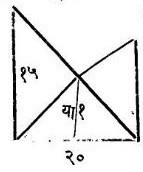
\includegraphics[scale=0.5]{Graphics/Capture4.JPG}
\end{minipage} 
\end{flushleft}

 अथ यावत्तावत्कल्पनां विनापि लम्बज्ञानार्थमाह~। अथवा वंशसम्बन्धिन्यौ 
आबाधे तद्युतिर्भूमिरित्यादि~। अयमर्थः यथावंशो महान् लघुर्वा भवति 
तथा तथा तदाश्रिता आबा-धापि महती लघ्वी भवति अतस्त्रैराशिकेनैवाबाधे 
ज्ञातुं शक्ये~। यथा~। यदि वंशयोगेन सकला भुर्लभ्यते तदा एकेन 
वंशेन किमिति पृथगाबाधे १२~। ८ अथ भूमितुल्ये २० भुजे लघुवंशः 
१० कोटिस्तदा बृहदाबाधाभुजे १२ केति लब्धो लम्बः ६ यतो लघुवंशः 
कोटिर्भूमिर्भुजो लघुवंशाग्रादितरवंशगामिसूत्रं कर्ण इत्येतत्क्षेत्रवशादेव बृहदाबाधाभुजो लम्बः कोटिरिति भवति~। एवं लब्धाबाधा बृहद्वंशाभ्यामप्यनुपातो 
द्रष्टव्यः~। अथ भूमिकल्पनं विनापि लम्बसिद्धिमाह~। अथवा वंशयोर्वधो
\newpage
%%%%%%%%%%%%%%%%%%%%%%%%%%%%%%%%%%%%%%%%%%%%%%%%%% 
\noindent योगहृतो यत्र तत्रापि वंशान्तरे लम्बः स्यादिति किं भूमिकल्पनयेति~। 
अत्रोपपत्तिः॥ \\
 
 \vspace{-3mm}
 यदि वंशयोगेन भूः लभ्यते तदा बृहद्वंशेन किम् इति लब्धा बृहद्वंशाश्रिताबाधा $\begin{matrix}
\vspace{-1mm}
\mbox{{भू ० वृ १}}\\
\vspace{-1.5mm}
\mbox{{व ० या १}}
\vspace{1mm}
\end{matrix}$~। अथ भूमितुल्ये भुजे लघुवंशः कोटिस्तदा बृहदाबाधायाः किमिति जातो लम्बः $\begin{matrix}
\vspace{-1mm}
\mbox{{भू १० ल १}}\\
\vspace{-1.5mm}
\mbox{{वं यौ}}
\vspace{1mm}
\end{matrix}$ अत्र भाज्यभाजकयोर्भूम्यपवर्ते जातम्~। $\begin{matrix}
\vspace{-1mm}
\mbox{{बृ ० ल १}}\\
\vspace{-1.5mm}
\mbox{{वं यो १}}
\vspace{1mm}
\end{matrix}$ एवमुपपन्नं वंशयोर्वधयोगहृतो लम्बः स्यादिति~॥ 

\begin{quote}
    \qt
     दैवज्ञवर्यगणसन्ततसेव्यपार्श्व- \\

\vspace{-7mm}
\hspace{1cm} बल्लालसञ्ज्ञगणकात्मजनिर्मितेऽस्मिन्~। \\

\vspace{-7mm}
 बीजक्रियाविवृतिकल्पलतावतारेऽ- \\

\vspace{-7mm}
\hspace{1cm} भूदेकवर्णजसमीकरणैकखण्डः~॥~७~॥
\end{quote}

\begin{center}
इति श्रीसकलगणकसार्वभौमश्रीबल्लालदैवज्ञसुतश्रीकृष्णदैवज्ञविरचिते \\
बीजविवृतिकल्पलतावतारे एकवर्णसमीकरणखण्डस्य विवरणम्~॥ 
\end{center}

\vspace{8mm}
\begin{figure}[h!]
    \centering
    
\includegraphics[scale=0.8]{Graphics/Capture1.JPG}
\end{figure}
\newpage
%%%%%%%%%%%%%%%%%%%%%%%%%%%%%%%%%%%%%%%%%%%

\phantomsection \label{madhyama}
\begin{center}
    \textbf{\LARGE अथ मध्यमाहरणविवरणम् }
\end{center}
 
  \vspace{2mm}
 तदेवं समशोधनादिना यथैकस्मिन् पक्षे एकजातीयमव्यक्तमेव परपक्षे च 
व्यक्तमेव भवति अथापवर्तादिनोपायेन सम्पाद्य प्रश्नभङ्गं उक्तम्~। अथ 
यद्यपवर्तेनापि तथा न भवति तत्र मध्यमाहरणलक्षणमुपायान्तरमिन्द्रवज्रया 
उपजातिकाभ्यां चाह\textendash 
\begin{quote}
    \bs
 अव्यक्तवर्गादि यदावशेषं पक्षौ तदेष्टेन निहत्य किञ्चित्~। \\
 क्षेप्यं तयोर्येन पदप्रदः स्यादव्यक्तपक्षोऽस्य पदेन भूयः~॥~५८~॥\\ 

 \vspace{-5mm}
 व्यक्तस्य मूलस्य समक्रियैवमव्यक्तमानं खलु लभ्यते तत्~। \\
 न निर्वहश्चेद्धनवर्गवर्गेष्वेवं तदा ज्ञेयमिदं स्वबुद्ध्या~॥~५९~॥\\

\vspace{-5mm}
 अव्यक्तमूलर्णगरूपतोऽल्पं व्यक्तस्य पक्षस्य पदं यदि स्यात्~। \\
 ऋणं धनं तच्च विधाय साध्यमव्यक्तमानं द्विविधं क्वचित्तु~॥~६०~॥~
\end{quote}

एतानि सूत्राण्याचार्य एव व्याख्यातवान्~। अत्रोपपत्तिः~। \\

\vspace{-3mm}
 एकस्मिन्पक्षेऽव्यक्तमेव परपक्षे च व्यक्तमेव यदि भवति तर्हि 
तयोः समत्वात्तस्याव्यक्तस्य तद्व्यक्तं मानं भवतीति पूर्वमेवोक्तम्~।
किन्तु व्यक्तशेषस्य हरणार्थमव्यक्तशेषपृथक्स्थमपेक्षितमतस्तादृशं यथा भवति तथा 
यतितव्यम्~। तत्र समयोः पक्षयोः समक्षेपे समशुद्धौ वा समगुणके वा 
समहरे वा मूलग्रहणे वा घनादिकरणे वा न समत्वहानिरिति तु स्पष्टम्॥ \\

\vspace{-3mm}
 अथ यत्राव्यक्तवर्गादिकं स्यादेकपक्षे च रूपाण्येव तत्र मूलेन 
विना कदापि नाव्यक्तस्यापृथक्स्थितिः~। अतः पक्षयोः साम्याविरोधेन मूले 
ग्राह्ये~। तथा सति मूलयोरपि समत्वं स्यात्~। अत उक्तं पक्षौ तदेष्टेन 
निहत्य किञ्चित्तयोः पक्षयोः क्षेप्यं येन पदप्रदः स्यादिति~। 

\afterpage{\fancyhead[RE]{\textbf{बीजपल्लवे}}}
\afterpage{\fancyhead[LO]{\textbf{मध्यमाहरणविवरणम्}}}
\afterpage{\fancyhead[RO,LE]{\textbf{\thepage}}}
\cfoot{}
\thispagestyle{empty} \newpage%%%%%%%%%%%%%%%%%%%%%%%%%%%%%%%%%%%%%%%%%%%%%%%%%% 

 अत्रेष्टेन निहत्येत्युपलक्षणम्~। क्वचित् इष्टेन पक्षावपवर्तनीयौ क्वचित् इष्टं 
पक्षयोः शोध्यमित्याद्यपि ध्येयम्~॥ \\

\vspace{-3mm}
 शेषोपपत्तिस्तु पूर्ववत्~। द्विविधमाने तु तत्रोदाहरणं वनान्तराले 
प्लवगाष्टभाग इति वक्ष्यमाणम्~। अत्र कपियूथं या १ अस्याष्टांशवर्गो 
द्वादशयुतो यूथसम इति समशोधने कृते जातौ पक्षौ $\begin{matrix}
\vspace{-1mm}
\mbox{या व १ या ६ं४ रू ०}\\
\vspace{-1.5mm}
\mbox{या व ० या ० रू ७६ं८}
\vspace{1mm}
\end{matrix}$~। पक्षयोर्द्वात्रिंशद्वर्गं १०२४ प्रक्षिप्य जातौ
$\begin{matrix}
\vspace{-1mm}
\mbox{या व १ या ६ं४ रू १०२४}\\
\vspace{-1.5mm}
\mbox{या व ० या ० रू २५६}
\vspace{1mm}
\end{matrix}$ अत्रोर्ध्वपक्षस्य पदमिदम्~। या १ रू ३ं२ इदं वा या १ं
रू ३२ द्वितीयपक्षस्य पदमिदं रू १६ पदयोः समशोधनार्थं न्यासः~। 
$\begin{matrix}
\vspace{-1mm}
\mbox{या १ रू ३ं२}\\
\vspace{-1.5mm}
\mbox{या ० रू १६}
\vspace{1mm}
\end{matrix}$ अयं वा $\begin{matrix}
\vspace{-1mm}
\mbox{या १ं रू ३२}\\
\vspace{-1.5mm}
\mbox{या ० रू १६}
\vspace{1mm}
\end{matrix}$ अतो द्विविधमपि मानमुपपद्यते ४८~। १६~।\\

 नन्वव्यक्तपदरूपेभ्यो व्यक्तपदेऽधिकेऽपि द्विविधं मानमनया युक्त्या 
कथं न स्यात्~। शृणु तर्हि~। अव्यक्तपक्षजरूपाणामृणत्वेऽव्यक्तस्य धनत्वमेव~।
अस्मिन्प्रकारेऽव्यक्तशेषस्य धनत्वार्थमव्यक्तपक्षरूपाण्येव व्यक्तपक्षाच्छोध्यानि~। 
तानि च धनं भवतीति नास्त्यनुप-पत्तिः~। अथ रूपाणां धनत्वेऽव्यक्तस्यर्णत्वमेवेति द्वितीयप्रकारेऽव्यक्तमेव धनत्वार्थमितरपक्षात् शोध्यम्~।
व्यक्तरूपाणि तु अव्यक्तपक्षजपदरूपेभ्यः शोध्यत्वादृणं भवति तानि यद्यधिकानि 
तदा ऋणं मानं स्यादिति द्वितीयं सर्वथाप्यनुपपन्नम्~॥\\

\vspace{-3mm}
 अत उक्तमव्यक्तमूलर्णगरूपतोऽल्पं व्यक्तस्य पक्षस्य पदं स्यादिति~। \\
 
 \vspace{-3mm}
 अथ यत्रालापे रूपोनमव्यक्तमस्ति तस्य वर्गे कर्तव्ये रूपाणामृणत्वादव्यक्तस्यर्णत्वमुत्पद्यते~। तत्र पदग्रहणे रूपाणामेव ऋणत्वं नाव्यक्तस्य 
आलापे रूपाणामृणत्वनिश्चयात्~। अव्यक्तस्यर्णत्वे कल्पिते ऋणं पक्षः
\newpage
%%%%%%%%%%%%%%%%%%%%%%%%%%%%%%%%%%%%%%%%%%%%%%%%%

\noindent स्यात्~। नह्यधिकस्य शोध्यत्वे धनं पक्षः सम्भवति~। भवतु वा क्वचिदस्य धनत्वं तथाप्यालापसिद्धपक्षादन्यथात्वं तु स्यादेव~। एवं सति आलापसिद्धपक्षसमेन द्वितीयपक्षेण कथमस्य साम्यं स्यात्~। अत समीकरणेनागतं 
मानमनुपपन्नमेव स्यात्~। ऋणत्वात्~। नहि व्यक्ते ऋणगते लोकस्य प्रतीतिरस्ति~। तस्मादेतादृश उदाहरणे व्यक्तपदेऽव्यक्तमूलर्णगरूपतोऽल्पेऽपि 
द्विविधं मानं न सम्भवति~। रूपाणां धनत्वकल्पनेन सिद्धस्य मानस्यानुपपन्नत्वात्~। एवमव्यक्तोनरूपवर्गे उद्दिष्टे सति तन्मूलेऽव्यक्तस्यैव ऋणत्वं न 
रूपाणाम्~। उक्तयुक्तेरविशेषात्~। अतस्तत्रापि द्विविधमानं न सम्भवति 
रूपाणामृणत्वकल्पनेन सिद्धस्य मानस्यानुपपन्नत्वात्~। इत्येवं बहुधा भवति~। 
क्वचित् क्षेपशोधनादिना शेषविधिना विपरीतमपि भवति~। क्वचिदव्यक्तस्य 
स्वतोऽप्यृणत्वे द्विविधमूलसम्भवेऽपि द्वितीयमनुपपन्नं भवति~। अत एवाचार्यैर्द्विविधं क्वचित्तदित्यनियमेनैवोक्तम्॥ \\

\vspace{-3mm}
 अथ द्वितीयमानस्यानुपपत्तौ वक्ष्यमाणमुदाहरणं प्रतीत्यर्थं प्रदर्श्यते~।
\begin{quote}
    \q
     "यूथात्पञ्चांशकस्त्र्यूनो वर्गितो गह्वरं गतः~। \\

\vspace{-7mm}
\hspace{1mm} दृष्टः शाखामृगः शाखामारूढो वद ते कति~॥"
\end{quote}

 अत्र यूथं या ५ अस्य पञ्चांशः या १ त्र्यूनः या १ रू ३ं 
वर्गितः या व १ या ६ं रू ९ दृष्टेन युतो या व १ या ६ं रू १० 
यूथसम इति शोधने कृते जातम्~। या व १ या १ं१~। रू १ं०~। पक्षौ 
चतुर्भिः सङ्गुण्य तयोरेकादशवर्गं क्षिप्त्वा जातो याव ४ या ४ं४ 
रू १२१~। ८१ अत्र रूपाणामेव ऋणत्वोद्देशादुक्तयुक्त्या पदमिदमेव~। या २ 
रू १ं१~। नेदं या २ं रू ११~। द्वितीयपक्षस्य पदम् रू ९~। पुनः 
समीकरणेन लब्धयावत्तावन्मानेन १० उत्थापितो जातो राशिः ५०~। 
रूपाणां धनत्वे तु यावत्तावन्मानमिदं १ राशिश्च ५ नह्यस्य पञ्चांशः १ 
त्रिभिरूनः सम्भवति~। एवमस्मिन्नेवोदाहरणे यूथात्पञ्चांशकस्त्रिच्युत इति
\newpage
%%%%%%%%%%%%%%%%%%%%%%%%%%%%%%%%%%%%%%%%%%%%%%%%%% 
\noindent यद्यालापः स्यात्तदा द्वितीयमानमेव युक्तं न तु पूर्वम्~। न हि पूर्वराशेः 
पञ्चांशः १० त्रिच्युतः सम्भवति~। अत एव\textendash 

\begin{quote}
    \qt
 द्युज्यकापमगुणार्कदोर्ज्यकासंयुतिं खखखबाणसंमितम्~। \\
 वीक्ष्य भास्करमवैहि मध्यमं मध्यमाहरणमस्ति चेद्यतम्~॥ 
\end{quote}

इत्यस्मिंस्त्रिप्रश्नोदाहरणे \,क्रान्तिज्यां \,यावत्तावन्मितां \,प्रकल्प्य \,ततोऽनुपातेन \,दोर्ज्या चानीय तयोर्योगमुद्दिष्टयुतेर्विशोध्य तद्वर्गं क्रान्तिज्यावर्गोनः 
त्रिज्यावर्गात्मकेन द्युज्यावर्गेण समं कृत्वा समशोधने कृते पक्षयोः 
पदग्रहणावसरेऽव्यक्तम् ऋणं रूपाणि धनम् इत्येव गृह्यतेऽत एव तदानयनसूत्रेऽपि 
तेन द्व्यूनो भवेदित्येवोक्तम्~। रूपाणामृणत्वे तु तेनाद्य आद्योऽयं
भवेदित्यप्युच्येत~। एवं मदुक्तयुक्त्या द्विविधमानोपपत्त्यनुपपत्ती सर्वत्रावधार्ये~।
तदेवमुपपन्नं द्विविधं क्वचित्तदिति~। पदग्रहणार्थं पक्षौ तदेष्टेन निहत्य किञ्चित् क्षेप्यं
तयोरित्युक्तं तत्र केन पक्षौ गुणनीयौ किं वा तयोः क्षेप्यमिति बालावबोधार्थं
श्रीधराचार्यकृतमुपायं दर्शयति~। चतुराहतवर्गसमरूपैः पक्षद्वयं गुणयेत्~।
पूर्वाव्यक्तस्य कृतेः समरूपाणि क्षिपेत्तयोरेवेति~। अस्यार्थः~। चतुर्गुणितेनाव्यक्तवर्गाङ्केन
पक्षद्वयं गुणयेत्~। गुणनात्प्राग्योऽव्यक्ताङ्कस्तद्वर्गतुल्यानि रूपाणि पक्षयोः क्षिपेत्~। 
एवं कृतेऽवश्यमव्यक्तपक्षस्य मूलं लभ्यते~। द्वितीयपक्षस्याप्येतन्समत्वान्मूलेन 
भाव्यम्~। एवं सति व्यक्तपक्षस्य यदि मूलं न लभ्यते तदा तत्खिलमेवेत्यर्थसिद्धम्~॥ \\

\vspace{-3mm}
 अत्र श्रीधराचार्यसूत्रे मूलोपायस्याव्यक्तवर्गाव्यक्तसापेक्षतयोक्तत्वाद्यत्रैकस्मिन्पक्षे अव्य-क्तवर्गोऽव्यक्तं च भवेत्तत्रैवास्य प्रवृत्तिरन्यत्र तु पदोपायः सुधिया स्वधिया चिन्त्यः~॥ \\

\vspace{-3mm}
 अथ श्रीधराचार्यसूत्रोपपत्तिः~। यत्र किल समशोधने कृते एकपक्षे 
अव्यक्तवर्गोऽव्यक्तं च स्तः~। इतरस्मिन्पक्षे रूपाण्येव सन्ति~। तत्र 
प्रथमपक्षे रूपयोगेन विना कथमपि न मूललाभः यतः केवलाव्यक्तस्य 
वर्गकरणेऽव्यक्तवर्ग एव स्यात्~। रूपयुताव्यक्तस्य
वर्गकरणेऽव्यक्तवर्गोऽव्यक्तं
\newpage%%%%%%%%%%%%%%%%%%%%%%%%%%%%
\noindent रूपाणि च स्युः~। प्रकृते त्वव्यक्तवर्गोऽव्यक्तं च तिष्ठतः~। स न 
कस्यापि वर्गः अतोऽवश्यं रूपाणि क्षेप्याणि~। यद्यप्यव्यक्तशोधनेनापि 
अव्यक्तवर्गमात्रस्य शेषत्वादव्यक्तपक्षस्य मूलं लभ्यते तथापि द्वितीयपक्षे तथा 
सति साव्यक्तानि रूपाणि स्युरिति नास्य मूललाभ इति पक्षयोः रूपाण्येव 
क्षेप्याणि~। तत्र यदाव्यक्तवर्गस्य मूलं लभ्यते तदा केवलं रूपाण्येव 
क्षेप्याणि~। यदा त्वव्यक्तवर्गस्य मूलं न लभ्यते तदाव्यक्तवर्गोऽपि तथा 
केनचिद्योज्यो गुणनीयो वा यथामूलं लभ्यते~। तत्राव्यक्तवर्गयोगे यद्यपि 
अव्यक्तपक्षस्य मूलं लभ्यते तथापि द्वितीयपक्षे साव्यक्तवर्गाणि रूपाणि 
स्युरित्यव्यक्तभावान्न मूललाभः~। न च पक्षयोरव्यक्तमपि क्षेप्यमिति वाच्यं
गौरवात्~। किं च यदव्यक्तपक्षेऽव्यक्तवर्गद्वयमस्ति तदा पक्षयोः किं 
क्षेप्यम्~। द्विसप्तचतुर्दशत्रयोविंशतिचतुस्त्रिंशत्सप्तचत्वारिंशत्द्विषष्ट्याद्यव्यक्तवर्गक्षेपे प्रथमपक्षस्यैव मूलं लभ्येत नेतरस्य~। एकं चतुराद्यव्यक्तवर्गक्षेपे 
तु प्रथमपक्षस्य मूलं न लभ्येत~। न च यत्राव्यक्तवर्गद्वयमस्ति तत्र 
पक्षयोरेकस्याव्यक्तवर्गस्य शोधनेन उभयोरपि मूलं लभ्यत इति वाच्यम्~। 
द्वितीयपक्षे ऋणस्याव्यक्तवर्गस्य मूलाभावात्~। न च त्रिपञ्चादिष्वव्यक्तवर्गेषु सत्सु एकचतुरादयोऽव्यक्तवर्गाः पक्षयोः क्षेप्याः द्विषडादि 
अव्यक्तवर्गेषु सत्सु पक्षौ द्विषडादिभिर्गुणनीयाविति वाच्यम्~। अगुणगमे 
सत्यननुगमस्यान्याय्यत्वात्~। क्रियानिर्वाहस्यानियतत्वाच्च~। अतिगौरवाच्च~।
यतोऽव्यक्तवर्गाव्यक्तरूपाणि तथा क्षेप्याणि यथोभयपक्षयोरपि मूलं लभ्येत~।
किञ्च मन्दावबोधार्थं ह्युपायकथनम्~। एतादृशस्य तु क्षेपस्य
मन्ददुर्ज्ञेयतयोपायकथनं व्यर्थमेव स्यात्~। तदेवं अव्यक्तवर्गः केनचिद्गुणनीय एवेति
सिद्धम्~। तत्र यदाव्यक्तवर्गस्य मूलं लभ्यते तदा रूपाण्येव क्षेप्याणि~। तानि 
कियन्तीति विचार्यते~। तत्र यद्यव्यक्तवर्गस्यैकमव्यक्तं मूलं लभ्यते तर्हि
अव्यक्तार्धवर्गक्षेपेऽव्यक्तपक्षस्यावश्यं मूललाभः यतः कृतिभ्य आदाय
पदानीत्यादि~। नाव्यक्तवर्गस्यैकमव्यक्तं मूलं रूपाणां त्वव्यक्तार्धतुल्या रूपाणि
द्वयोरभिहतिरव्यक्ततुल्यं स्यात्सा द्विघ्नी अव्यक्ततुल्या स्यादिति तच्छोधनेन निश्शेषता स्यात्~। एवं
\newpage
%%%%%%%%%%%%%%%%%%%%%%%%%%%%%%%%%%%%%%%%%%%%%%%%%% 

\noindent यत्राव्यक्तवर्गस्याव्यक्तद्वयं मूलं लभ्यते तत्राप्यनयैव युक्त्या
यथास्थिताव्यक्तचतुरंशवर्गतुल्यरूपक्षेपेऽव्यक्तं मूललाभः~। एवं यत्राव्यक्तत्रयं मूलं
लभ्यते तत्र पक्षस्थिताव्यक्त-षडंशवर्गतुल्यरूपक्षेपेऽवश्यं मूललाभः~। तथा च
यत्राव्यक्तवर्गस्य मूलं लभ्यते तत्र तेन मूलाङ्केन द्विगुणेन अव्यक्ताङ्के भक्ते यल्लभ्यते
तद्वर्गतुल्यानि रूपाणि क्षेप्याणीति सिद्धम्~॥ \\

\vspace{-3mm}
 अथ यत्राव्यक्तवर्गाङ्कस्य न मूलं लभ्यते तत्र तेनैवाङ्केन गुणे सत्यवश्यं
मूललाभ इति अव्यक्तवर्गाङ्केन पक्षौ गुणनीयौ~। अथात्र पूर्वयुक्त्या
रूपक्षेपः तदर्थमव्यक्तवर्गमूलाङ्केन द्विगुणेनाव्यक्ताङ्को भाज्यः~। अत्राव्यक्तवर्गमूलाङ्कस्तु 
अगुणितोऽव्यक्तवर्गाङ्कः~। तथा च गुणितेनाव्यक्तवर्गाङ्केन द्विगुणेन अव्यक्ताङ्को 
भाज्यः पक्षगुणकेन अगुणिताव्यक्तवर्गाङ्केनापवर्ते कृते जातः पूर्वाव्यक्ताङ्कस्य द्वयं 
भाजकः~। अतः पूर्वाव्यक्तार्धं वर्गतुल्यानि रूपाणि क्षेप्याणीति सिद्धम्~।
एवं यत्र विनैव गुणनं अव्यक्तवर्गाङ्कस्य मूलं लभ्यते~तत्राप्युक्त-युक्त्या \,पक्षावव्यक्तवर्गाङ्केन \,सङ्गुण्य \,पूर्वाव्यक्तार्धवर्गतुल्यानि \,रूपाणि \,प्रक्षिप्य \,च \,मूलं लभ्यत एव~॥ \\

\vspace{-3mm}
 युक्तेरविशेषात्~। तदेवं पक्षौ अव्यक्तवर्गाङ्केन गुण्यो पूर्वाव्यक्तार्धवर्गतुल्यानि 
रूपानि तयोः क्षेप्यानि चेति सिद्धम्~। एतावतेव पक्षयोर्मूललाभे सिद्धेऽपि
अभिन्नत्वार्थं पुनश्चतुर्भिः गुणनमुक्तम्~। यतो वर्गेण वर्गगुणने कृते
नास्ति वर्गत्वहानिः~॥ \\

\vspace{-3mm}
 अथात्र पूर्वयुक्त्याक्षेपः~। अत्राव्यक्तवर्गे चतुर्भिर्गुणिते तन्मूलाङ्को 
द्विगुणितः स्यात्~। तेन \,च \,द्विगुणेनाव्यक्ताङ्को \,भाज्य \,इति \,जातः \,पूर्वाव्यक्तस्य \,पूर्वाव्यक्तवर्गाङ्कश्चतुर्गुणो भाजकः~। पक्षगुणकोऽपि तावानेवास्तीति
गुणहरयोस्तुल्यत्वान्नाशे पूर्वाव्यक्तवर्गतुल्यानि रूपाणि क्षेप्याणीति सिद्धम्~॥ 
तदेवमुपपन्नं चतुराहतवर्गसमैः रूपैः पक्षद्वयं गुणयेत्~। पूर्वाव्यक्तस्य कृतेः 
समरूपाणि क्षिपेत्तयोरेवेति~। एवं कृतेऽपि यदि व्यक्तपक्षस्य मूलं न 
लभ्यते तदा करण्यात्मकं मूलं ग्राह्मम्~॥
\newpage%%%%%%%%%%%%%%%%%%%%%%%%%%%%
 अथात्र शिष्यबुद्धिप्रसादार्थं विविधान्युदाहरणानि निरूपयन्नेकमुदाहरणं 
मालिन्याह\textendash 
\begin{quote}
    \ex
    अलिकुलदलमूलं मालतीं यातमष्टौ \\

\vspace{-7mm}
\hspace{1cm} निखिलनवमभागाश्चालिनीभृङ्गमेकम्~। \\

\vspace{-7mm}
 निशि परिमललुब्धं पद्ममध्ये निबद्धं \\

\vspace{-7mm}
\hspace{1cm} प्रतिरणतिरणन्तं ब्रूहि कान्तेऽलिसङ्ख्याम्~॥~६२~॥~
\end{quote}

स्पष्टोऽर्थः~। अत्रालिकुलप्रमाणं द्विगुणवर्गात्मकं कल्पयन्तोऽस्यैव दलमूलं
सम्भवति~। अतस्तथा कल्पितमाचार्यैः या व २ गणितमाकरे स्फुटम्~। 
जातालिकुलसङ्ख्या ७२~। अथान्यदुदाहरणं शार्दूलविक्रीडितेनाह\textendash 
\begin{quote}
    \ex
    पार्थः कर्णवधाय मार्गणगणं क्रुद्धो रणे सन्दधे \\
 तस्यार्धेन निवार्य तच्छरगणं मूलैश्चतुर्भिर्हयान्~। \\
 शल्यं षड्भिरथेषुभिस्त्रिभिरपि च्छत्रं ध्वजं कार्मुकं \\
 चिच्छेदास्य शिरः शरेण कति ते यानर्जुनस्सन्दधे~॥~६३~॥~ 
\end{quote}

स्पष्टोऽर्थः~। अत्र कल्पितं बाणमानं याव १ अस्यार्धं याव $\begin{matrix}
\vspace{-2mm}
\mbox{{१}}\\
\vspace{-1.5mm}
\mbox{{२}}
\vspace{1mm}
\end{matrix}$ चत्वारि मूलानि या ४~। दृश्यबाणगणश्च रू १०~। एषामैक्यं याव $\begin{matrix}
\vspace{-2mm}
\mbox{{१}}\\
\vspace{-1.5mm}
\mbox{{२}}
\vspace{1mm}
\end{matrix}$ या ४ रू १० राशि\textendash \,या व १\textendash \,समं कृत्वा पक्षौ समछेदीकृत्य छेदगमे शोधने च कृते पक्षयोः षोडशरूपाणि प्रक्षिप्य मूले गृहीत्वा पुनः समीकरणेन लब्धं यावत्तावन्मानं १० जाता बाणसङ्ख्या १००~॥ \\

\vspace{-3mm}
 अथान्यदुदाहरणमुपजातिकयाह\textendash 
\begin{quote}
    \ex
     व्येकस्य गच्छस्य दलं किलादिः \\

\vspace{-7mm}
\hspace{1cm} आदेर्दलं तत्प्रचयः फलं च~। \\

\vspace{-7mm}
 चयादिगच्छाभिहतिः स्वसप्त- \\

\vspace{-7mm}
\hspace{1cm} भागाधिका ब्रूहि चयादिगच्छान्~॥~६४~॥
\end{quote}
 \newpage%%%%%%%%%%%%%%%%%%%%%%%%%%%%%%%%%%%%%%%%%%%%%%%%%% 

\noindent फलं चेति चस्त्वर्थे~। तथा सति फलशब्दस्योत्तरार्धेन अन्वयः सुबोधः~। शेषं स्पष्टम्~। अत्र गच्छमानं यावत्तावच्चतुष्टयं रूपाधिकम्~। या ४ रू १ 
प्रकल्प्य गणितमाकरे स्फुटम्~। द्वितीयप्रकारेण फलसाधनार्थं पाटीस्थं सूत्रमिदम्~॥ 

\begin{quote}
{\qt "व्येकपदघ्नचयो मुखयुक् स्यादन्त्यधनं मुखयुग्दलितं तत्~। \\
मध्यधनं पदसङ्गुणितं तत्सर्वधनं गणितञ्च तदुक्तम्"}\renewcommand{\thefootnote}{*}\footnote{लीलावत्यां श्रेढीव्यवहारे श्लोकम् ३७ इति~॥}
\end{quote}

 अथान्यदुदाहरणमनुष्टुभाह\textendash 
\begin{quote}
    \ex
     कः खेन विहृतो राशिराद्यौ युक्तोऽथवोनितः~। \\
 वर्गितः स्वपदेनाढ्यः खगुणो नवतिर्भवेत्~॥~६५~॥~
\end{quote}

स्पष्टोऽर्थः~। अत्र राशिः या १ अयं खहृतः या $\begin{matrix}
\vspace{-1.5mm}
\mbox{१}\\
\vspace{-1.5mm}
\mbox{०}
\vspace{1mm}
\end{matrix}$ अयमाद्यौ युक्त ऊनितो वाविहृत एव खहरत्वात्~। अथायं~। या
$\begin{matrix}
\vspace{-1.5mm}
\mbox{१}\\
\vspace{-1.5mm}
\mbox{०}
\vspace{1mm}
\end{matrix}$ वर्गितः~। या व $\begin{matrix}
\vspace{-1.5mm}
\mbox{१}\\
\vspace{-1.5mm}
\mbox{०}
\vspace{1mm}
\end{matrix}$ स्वपदेन या $\begin{matrix}
\vspace{-1.5mm}
\mbox{१}\\
\vspace{-1.5mm}
\mbox{०}
\vspace{1mm}
\end{matrix}$ युक्तः या व $\begin{matrix}
\vspace{-1.5mm}
\mbox{१}\\
\vspace{-1.5mm}
\mbox{०}
\vspace{1mm}
\end{matrix}$~या~$\begin{matrix}
\vspace{-1.5mm}
\mbox{१}\\
\vspace{-1.5mm}
\mbox{०}
\vspace{1mm}
\end{matrix}$ \,अयं \,खगुणितो \,जातः~। या व १ या १ \,गुणहरयोस्तुल्यत्वेन \,नाशात्~। अथायं नवतिसमं कृत्वा समशोधने कृते 
पक्षौ चतुर्भिः सङ्गुण्य रूपं प्रक्षिप्य प्राग्वज्जातो राशिः ९~॥ \\

\vspace{-3mm}
 अन्यदुदाहरणमनुष्टुभाह\textendash 
\begin{quote}
    \ex
    कः स्वार्धसहितो राशिः खगुणो वर्गितो युतः~। \\
 स्वपदाभ्यां खभक्तश्च जातः पञ्चदशोच्यताम्~॥~६६~॥~
\end{quote}
 
स्पष्टोऽर्थः~। अत्र राशिः या १ गणितमाकरे स्फुटम्~। मूलार्थं रूपचतुष्टयं क्षेपः~॥ 
\newpage%%%%%%%%%%%%%%%%%%%%%%%%%%%%
 अन्यदुदाहरणमार्ययाह\textendash 
\begin{quote}
    \ex
     राशिर्द्वादशनिघ्नो राशिघनाढ्यश्चैकः समा यस्य~। \\
 राशिकृतिः षड्गुणिता पञ्चत्रिंशद्युता विद्वन्~॥~६७~॥~
\end{quote}
 
स्पष्टोऽर्थः~। गणितमाकरे स्फुटम्~॥ \\

\vspace{-3mm}
 अथान्यदुदाहरणं सार्धानुष्टुभाह\textendash 
\begin{quote}
    \ex
     को राशिर्द्विशतीक्षुण्णो राशिवर्गयुतो हतः~। \\
 द्वाभ्यां तेनोनितो राशिर्वर्गवर्गोऽयुतं १०००० भवेत्~॥~६८~॥~\\

\vspace{-5mm}
 रूपोनं वदतं राशिं वेत्सि बजिक्रियां यदि 
\end{quote}

 स्पष्टोऽर्थः~। रूपोनमयुतं भवेदिति योजनीयम्~। राशिः या १ अस्य 
यथोक्ते समशोधने कृते पक्षयोः या व ४ या ४०० रू १ एतावत्क्षिप्त्वा 
गणितमाकरे स्फुटम्॥ \\

\vspace{-3mm}
 अथाव्यक्तमूलर्णगरूपतोऽल्पमित्यस्य सूत्रस्योदाहरणमुपजातिकयाह\textendash 
\begin{quote}
    \ex
     वनान्तराले प्लवगाष्टभागः \\
 संवर्गितो वल्गति जातरागः~। \\
 ब्रूत्कारनादप्रतिनादहृष्टा \\
 दृष्टा गिरौ द्वादश ते कियन्तः~॥~६९~॥~
\end{quote}
 
प्लवगाः वानराः ब्रूदिति तन्नादानुकृतिः~। शेषं स्पष्टम्~। गणितमाकरे 
स्फुटम्~। द्विधा मानं चैतत् ४८~। १६॥ \\

\vspace{-3mm}
 अथ द्विधा मानस्य क्वचित्कत्वप्रदर्शनार्थमुदाहरणद्वयमनुष्टुब्द्वयेनाह\textendash 
\begin{quote}
    \ex
यूथात्पञ्चांशकस्त्र्यूनो वर्गितो गह्वरं गतः~। \\
 दृष्टः शाखामृगः शाखामारूढो वद ते कति~॥~७०~॥
 \end{quote}

\newpage
%%%%%%%%%%%%%%%%%%%%%%%%%%%%%%%%%%%%%%%%%%%%%%%%%% 
\begin{quote}
    \ex
    कर्णस्य त्रिलवेनोना द्वादशाङ्गुलशङ्कुभा~। \\
 चतुर्दशाङ्गुला जाता गणक ब्रूहि तां द्रुतम्~॥~७१~॥~
\end{quote}
 
त्रिभिरूनस्त्र्यूनः~। शाखामृगो वानरः~। स्पष्टमन्यत्~। गणितमाकरे स्पष्टम्~॥\\

\vspace{-3mm}
 अथान्यदुदाहरणमनुष्टुब्द्वयेनाह\textendash
\begin{quote}
    \ex
     चत्वारो राशयः के ते मूलदा ये द्विसंयुताः~। \\
 द्वयोर्द्वयोर्यथासन्नघाताश्चाष्टादशान्विताः~॥~७२~॥~\\

\vspace{-5mm}
 मूलदाः सर्वमूलैक्यादेकादशयुतात्पदम्~। \\
 त्रयोदश सखे जातं बीजज्ञ वद तान्मम~॥~७३~॥~
\end{quote}

स्फुटोऽर्थः~। अत्रोदाहरणे राशीनामव्यक्तकल्पने क्रिया न निर्वहति~। अत
एकं मूलं यावत्तावत्प्रकल्प्य यथा सर्वमूलानि सिध्यन्ति तथा निरूपयति~। 
तत्र राशिमूलकल्पनार्थमाह~। अत्र राशिः येन युतः मूलदः भवति 
स किल राशिक्षेपः~। मूलयोरन्तरवर्गेण हतो राशिक्षेपो वधक्षेपो भवति~। 
तयोः राश्योर्वधस्तेन युतोऽवश्यं मूलदः स्यादित्यर्थ इति~॥ \\

\vspace{-3mm}
 नन्वनेन ग्रन्थेन राशिमूलकल्पनं कथमुक्तम्~। श्रुणु मूलयोरन्तरवर्गेण 
हतो राशिक्षेपो वधक्षेपो भवतीत्यनेन राशिक्षेपस्य मूलान्तरवर्गस्य च वधो 
वधक्षेपोऽस्तीति स्पष्टीकृतम्~॥ तथा च राशिक्षेपेण वधक्षेपे भक्ते यल्लभ्यते 
स एव मूलान्तरवर्गः अतस्तस्य पदं मूलान्तरं स्यात्~। अतो यावत्तावदात्मकं प्रथममूलं तेन मूलान्तरेण युक्तं सत् द्वितीयं मूलं स्यात्~। तदपि 
पुनस्तेनैव युक्तं सत् तृतीयं स्यादित्यादि~। इदमेवोक्तमाद्यपरिभाषायामपि~।
राशिक्षेपाद्वधक्षेपो यद्गुणस्तत्पदोत्तरम्~। अव्यक्तराशयः कल्प्या इति~। 
अत्राव्यक्तराशयो राशिमूलान्येव~। अत एवैभ्यो राशिज्ञानमुक्तं चतुर्थचरणेन~।
वर्गिताः क्षेपवर्जिता इत्यनेन~। यतो राशिः क्षेपेण योज्यः तस्य मूलं 
राशिमूलं भवत्यतो व्यस्तविधिना राशिमूलं वर्गितं क्षेपोनं सद्राशिर्भवेदित्यर्थः~।
\newpage%%%%%%%%%%%%%%%%%%%%%%%%%%%%१९५ 
 अथैतेभ्यो वधमूलान्याह~॥ राशिमूलानां यथासन्नं द्वयोर्द्वयोर्वधाः 
राशिक्षेपोना राशि-वधमूलानि भवन्तीति~॥ स्पष्टोऽर्थः~॥ अत्रोभयत्रोपपत्तिरुच्यते~। 
अत्र क्षेपयुतराशेर्मूले ज्ञाते व्यस्तविधिना मूलवर्गे क्षेपोने राशिर्भवेदिति जातं प्रथममूलात्प्रथमराशिः प्रमूव १ क्षे १ं एवं द्वितीयमूलात् द्वितीयोऽपि~। द्विमूव १ क्षे १ं अनयोर्वधो येन युक्तः सन्मूलदो भवेत्स एव व क्षेपः 
तदर्थमनयोर्गुणनार्थं न्यासः प्र मू $\begin{matrix}
\vspace{-1mm}
\mbox{व १}\\
\vspace{-1.5mm}
\mbox{क्षे १ं}
\vspace{1mm}
\end{matrix}$~। $\begin{matrix}
\vspace{-1mm}
\mbox{द्वि मू व १ क्षे १ं}\\
\vspace{-1.5mm}
\mbox{द्वि मू व १ क्षे १ं}
\vspace{1mm}
\end{matrix}$ गुणनाज्जातं~। प्र मू व ० द्वि मू व १ प्रमूव क्षे १ं द्विमूव क्षे १ं क्षे व १~॥ \\

\vspace{-3mm}
 अत्र द्वितीयखण्डे क्षेपगुणः प्रथममूलवर्गः ऋणमस्ति तृतीयखण्डे 
क्षेपगुणो द्वितीयमूलवर्गः ऋणमस्ति~। अत्र लाघवान्मूलवर्गयोगः क्षेपगुणः 
ऋणमिति न्यासः प्रमूव ० द्विमूव १ मूव यो ० क्षे १ं क्षे व १~। 
अत्राद्यखण्डे मूलवर्गघातोऽस्ति य एव मूलवर्गघातः स एव मूलघातवर्ग 
इति तथा न्यासः~। मूघा व १ मूव यो १ क्षे १ं क्षे व १~। अत्र 
द्वितीयखण्डे मूलवर्गयोगः क्षेपगुणोऽस्ति~। तत्र मूलवर्गयोगस्य खण्डद्वयम्~।
एकं मूलान्तरवर्गः अपरं मूलयोर्द्विघ्नो घातः~। राश्योरन्तरवर्गेण द्विघ्ने घाते 
युते तयोः वर्गयोगो भवेदित्युक्तत्वात्~। अतो जाते वर्गयोगस्य खण्डे~। 
मू अं व १ मूघा २ अनयोः क्षेपेण गुणने जातं द्वितीयखण्डं खण्डद्वयात्मकम्~। मू अं व ० क्षेपं १ मूघा ० क्षे २ं सर्वेषां खण्डानां क्रमेण 
न्यासः मूघा व १ नू अं व ० क्षे १ं मूघा ० क्षे २ं क्षे व १~। अयं
हि राशिवधः~। अयं येन युतः सन्मूलदः स्यात्स एव वधक्षेपः~। अत्र
क्षेपगुणे मूलान्तरवर्गे क्षिप्ते शेषस्यास्य~। मूघा व १ मूघा ० क्षे २ं क्षेव १~।
कृतिभ्य आदाय पदानीत्यादिना पदमिदमायाति~। मूघा १ क्षे १ं इदं
हि वधमूलम्~। अत उपपन्नं मूलयोरन्तरवर्गेण हतो राशिक्षेपो वधक्षेपो
भवतीति~। राशिमूलानां यथासन्नं द्वयोर्द्वयोर्वधराशिक्षेपोना वधमूलानि भवन्ति इत्यपि~॥
 \newpage%%%%%%%%%%%%%%%%%%%%%%%%%%%%%%%%%%%%%%%%%%%%%%%%%% 

 अनयैव युक्त्या द्वितीयतृतीययोस्तृतीयचतुर्थयोरपि राश्योर्वधमूलोपपत्तिः द्रष्टव्या~॥ एवमेकं राशिमूलं यावत्तावत्प्रकल्प्य ततः सर्वमूलसिद्धिरुक्ता~। अथ प्रकृतोदाहरणे योज-यति~। अत्रोदाहरणे राशिक्षेपाद्वधक्षेपो नवगुणो नवानां च मूलं त्रयोतस्त्र्युत्तराणि राशिमूलानीत्यादिना~। शेषं स्पष्टम्~॥ \\

\vspace{-3mm}
 अथान्यदुदाहरणमनुष्टुभाह\textendash
\begin{quote}
    \ex
      क्षेत्रे तिथिनखैस्तुल्ये दोः कोटी तत्र का श्रुतिः~। \\
 उपपत्तिश्च रूढस्य गणितस्यास्य कथ्यताम्~॥~७४~॥~
\end{quote}

तत्कृत्योर्योगपदं कर्ण इति रूढस्य प्रसिद्धगणितस्योपपत्तिः कथ्यताम्~॥ 
उपपत्तिमेव प्रष्टुमत्र श्रुतिप्रश्नो द्रष्टव्यः~। अत्र कर्णः या १ क्षेत्रदर्शनम्~। \raisebox{-0.45\height}{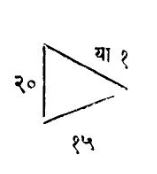
\includegraphics[scale=0.8]{Graphics/Capture15.JPG}} अत्र कर्णस्य भूमित्वकल्पने दर्शनम्~। \raisebox{-0.45\height}{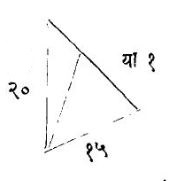
\includegraphics[scale=0.7]{Graphics/Capture16.JPG}} क्षेत्रं परिवर्त्य दर्शनम्~। \raisebox{-0.45\height}{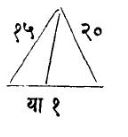
\includegraphics[scale=0.8]{Graphics/Capture17.JPG}} अत्र लम्बादुभयतो ये त्र्यस्रे तयोरपि भुजकोटी पूर्वभुजकोट्यनुरूपे भवतः~। तत्र भुजाश्रिता आबाधा भुजः लम्बः कोटिः पूर्वभुजः कर्ण इत्येकं त्र्यस्रम्~। लम्बो भुजो द्वितीयाबाधा कोटिः पूवकोटिः

\newpage%%%%%%%%%%%%%%%%%%%%%%%%%%%%१९७ 

\noindent २० कर्ण इत्यपरम्~। नन्वत्र त्र्यस्रद्वयेऽपि लम्ब एव कथं न कोटिः~। 
सत्यम्~। दोःकोट्यो नामभेदोनस्वरूपभेद इति यद्यप्यस्ति तथापि प्रकृते 
भुजकोट्योः पूर्वभुजकोट्यनुरूपत्वविवक्षया न तथा~। पूर्वं हि भुजात्कोटिर्महतीति प्रकृतेऽपि तथैव भाव्यम्~। किञ्च प्रकृतभुजकोट्योः पूर्वभुजकोट्यनुरूपत्वे विवक्षिते सति भुजतुल्ये कर्णे यदि लम्बः कोटिस्तदाकोटितुल्ये कर्णे केति त्रैराशिकेन कोटिभेदेन भाव्यम्~। यद्वा परस्परस्पर्धिदिशोर्भुजयोरेकतरस्य कोटिरिति सञ्ज्ञा स्वेच्छया क्रियताम्~। परं यावत्तावति कर्णे यदि विंशतिमिताकोटिस्तदा विंशतिमिते कर्णे का कोटिरिति त्रैराशिकेन विंशतिमिते कर्णे परस्परस्पर्द्धिदिशोर्भुजयोर्मध्ये महानेव भुज आबाधरूपः सिद्ध्येन्न तु लम्बरूपो लघुभुजः~। प्रमाणभुजस्य महत्वात्~। एवं यावत्तावति कर्णे यदि पञ्चदशमितो भुजस्तर्हि पञ्चदशमिते कर्णे को भुज इति 
पञ्चदशमितिकर्णे परस्परस्पर्द्धिदिशोर्भुजयोर्मध्ये लघुरेव भुज आबा-धरूपः
सिद्ध्येन्न तु लम्बरूपो महान्भुजः प्रमाणभुजस्य लघुत्वात्~। तदेवं यत्र 
कुत्रापि जात्ये त्र्यस्रे यदि यावत्तावत्कर्णो भुजः कल्प्यते तर्हि यावत्तावति 
कर्णे भुजो भुजस्तदा भुजतुल्ये कर्णे क इति त्रैराशिकेन या १~। 
भु १ भु १ भुजाश्रिता आबाधा सिद्ध्येत् $\begin{matrix}
\vspace{-1mm}
\mbox{भुव १}\\
\vspace{-1.5mm}
\mbox{या १}
\vspace{1mm}
\end{matrix}$~। एवं यावत्तावति कर्णे यदि कोटिः 
कोटिस्तदा कोटितुल्ये कर्णे केति त्रैराशिकेन या १~। को १~। को १ 
कोट्याश्रिता आबाधा सिद्ध्येत्~। को $\begin{matrix}
\vspace{-1mm}
\mbox{व १}\\
\vspace{-1.5mm}
\mbox{या १}
\vspace{1mm}
\end{matrix}$~। आबाधयोर्योगोऽयम्~। भु $\begin{matrix}
\vspace{-1mm}
\mbox{व १}\\
\vspace{-1.5mm}
\mbox{या १}
\vspace{1mm}
\end{matrix}$ को व १~। अयं भूम्यानया या १ सम इति पक्षौ समच्छेदीकृत्य छेदगमे जातौ $\begin{matrix}
\vspace{-1mm}
\mbox{या व १}\\
\vspace{-1.5mm}
\mbox{भुव १ को व १ }
\vspace{1mm}
\end{matrix}$ अत्र पक्षयोः समत्वात् य एव यावद्वर्गः स एव 
भुजकोटिवर्गयोग इति सिद्धम्~। प्रकृते कर्णो यावत्तावदात्मकोऽस्तीति यावत्तावद्वर्गः 
कर्णवर्ग एव~। तस्मात्सिद्धं य एव कर्णवर्गः स एव भुजकोटिवर्गयोग 
इति~। अतोऽस्य पदं कर्णो भवितुमर्हति~। अत उपपन्नं तत्कृत्यो-
\newpage%%%%%%%%%%%%%%%%%%%%%%%%%%%%%%%%%%%%%%%%%%%%%%%%%% 

\noindent र्योगपदं कर्ण इति~। अथवान्यथोपपत्तिः~। उद्दिष्टक्षेत्रमिदम्~। \raisebox{-0.45\height}{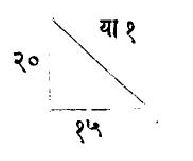
\includegraphics[scale=0.65]{Graphics/Capture13.JPG}} कर्णो यथा बहिर्भवति तथैतत्सममन्यत् योज्यते~॥ दर्शनम्~। \raisebox{-0.45\height}{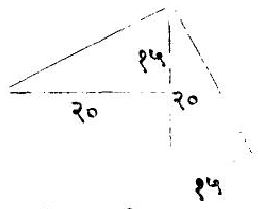
\includegraphics[scale=0.55]{Graphics/Capture14.JPG}}\\

\vspace{1mm}
अथैवमेव तृतीयक्षेत्रं योज्यते~। एवं चतुर्थक्षेत्रयोगदर्शनम्~। एवं समजात्यचतुष्टयेन
 
\begin{figure}[h!]
    \centering
    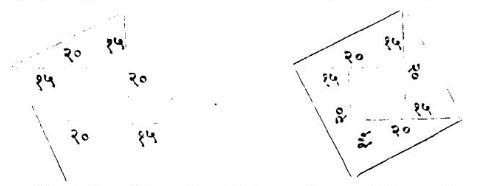
\includegraphics[scale=0.8]{Graphics/Capture12.JPG}
\end{figure}

\noindent तद्भुजकोट्यन्तरसमचतुर्भुजेन समकर्णेन पञ्चमेन चेति पञ्चभिः क्षेत्रैरेकं समकर्णं समचतुर्भुजं क्षेत्रं भवति~। यत्तु समजात्यचतुष्टयमात्रेण च समचतुर्भुजं भवति तद्विषमकर्णमेव~। \\

\vspace{-3mm}
 अथ प्रकृते समकर्णे विषमकर्णे च समचतुर्भुजत्र्यस्रकर्णतुल्या एव 
भुजाः~। परं समकर्णे चतुर्भुजे भुजकोट्यन्तरसमचतुर्भुजं क्षेत्रमधिकमस्ति~।
अत एव भुजसमत्वेऽपि यथा यथा कर्णवैषम्यं भवति तथा तथा क्षेत्रसङ्कोचात् 
क्षेत्रफलमल्पं भवतीति प्रतिपादितमाचार्यैर्लीलावत्याम्॥ \\

\vspace{-3mm}
 अथ प्रकृतमनुसरामः~। अत्र समकर्णे समचतुर्भुजे क्षेत्रे समश्रुतौ 
तुल्यचतुर्भुजे च तथायते तद्भुजकोटिघात इति अनेन भुजकोटिघातः फलं 
भवति~। अत्र भुजकोट्योः समतया भुजकोटिघातः समद्विघातो  भवतीति 
भुजवर्ग एव क्षेत्रफलम्~। अतः क्षेत्रफले ज्ञाते सति तन्मूलं भुजमानं 
स्यात् चतुर्भुजे यो भुजः स एव त्र्यस्रे कर्णोऽस्तीति कर्णोऽपि ज्ञातः

\newpage%%%%%%%%%%%%%%%%%%%%%%%%%%%%१९९ 

\noindent स्यात्~। अतः क्षेत्रफलं खण्डैः साध्यते~। तत्र त्र्यस्रे भुजकोटिघातार्थं
फलं भवतीति जातमेकस्मिंस्त्र्यस्रे क्षेत्रफलं भुवको $\begin{matrix}
\vspace{-1.5mm}
\mbox{१}\\
\vspace{-1.5mm}
\mbox{२}
\vspace{1mm}
\end{matrix}$ इदं चतुर्गुणं सत् त्र्यस्त्रचतुष्टयस्य फलं स्यादिति जातं भुवको २~। भुजकोट्यन्तरसमचतुर्भुजस्य क्षेत्रस्योक्तयुक्त्या भुजकोटयन्तरवर्गः फलं स्यात्~। तत्र भुजकोट्यन्तरमिदं भुज १ं को १ अस्य वर्गः स्थाप्योऽन्त्यवर्ग इत्यादिना यद्वा खण्डगुणनेन जातः भुव १ भु ० को २ं को व १~। इदमन्तर्लघुचतुर्भुजस्य क्षेत्रस्य फलं त्र्यस्रचतुष्टयफलेनानेन भु ० को २ युतं सज्जातं प्रकृतचतुर्भुजस्य फलं भुव १ को व १ एवं भुजकोट्योर्द्विघ्नो घातो भुजकोट्यन्तरवर्गेण युतः सन् 
भुजकोटिवर्गयोगो भवति~। एतदेवाहानुष्टुभा\textendash 
\begin{quote}
    \bs
   दोःकोट्यन्तरवर्गेण द्विघ्नो घातः समन्वितः~। \\
 वर्गयोगस्समः स स्यात् द्वयोरव्यक्तयोर्यथा~॥~६१~॥~
 
\end{quote}
 
तत्र दोःकोटी उपलक्षणम्~। अत एव चतुर्भुजे भुजः स्यात्~। सम एव 
त्र्यस्रे कर्णे इति वोपपन्नं तत्कृत्योर्योगं पदं कर्ण इति~॥ \\

\vspace{-3mm}
 अथान्यदुदाहरणमनुष्टुभाह\textendash 
\begin{quote}
    \ex
     भुजात्त्र्यूनात्पदं व्येकं कोटिकर्णान्तरं सखे~। \\
 यत्र तत्र वद क्षेत्रे दोःकोटिश्रवणान्मम~॥~७५~॥~
\end{quote}

स्पष्टोऽर्थः~। अत्र कोटिकर्णान्तरमिष्टं कल्पितं २ भुजात्त्र्यूनात्पदं व्येकं सत् 
कोटि-कर्णान्तरं भवत्यतो विलोमविधिना कोटिकर्णान्तरं २ सैकं ३ वर्गितं ९ 
त्रियुतं जातो भुजः \,१२ \,अस्य \,वर्गः \,कोटिकर्णयोर्वर्गान्तरं \,१४४ \,यतो \,भुजकोट्योर्वर्गरूपः \,कर्णवर्गो रूपतः कर्णवर्गात्कोटिवर्गेऽपनीते भुजवर्ग एव अवशिष्यते~। अतो योऽयं भुजवर्गः १४४ तत्कोटिकर्णयोर्वर्गान्तरम्~। कल्पितकोटिकर्णान्तरमिदम् २ अतो वर्गान्तरं राशिवियोगभक्तं योग इति जातः कोटिकर्णयोगः ७२ योगान्तराभ्यां योगोऽन्तरेणोनयुतोर्द्धित इति सङ्क्रमणसूत्रेण जातौ कोटिकर्णौ ३५~। ३७ एवं कोटिकर्णान्तरमेकं १ प्रकल्प्योक्तवज्जाता भुजकोटिकर्णाः ७~। २४~। २५ एवमनेकधा~॥
 \newpage%%%%%%%%%%%%%%%%%%%%%%%%%%%%%%%%%%%%%%%%%%%%%%%%%% 
 अथ वर्गान्तरं राशिवियोगभक्तं योग इत्यत्रोपपत्तिः~। वर्गान्तरं हि 
योगान्तरघातोऽस्ति~। अतो यस्मिन्नन्तरेण भक्ते योगो लभ्येत तेनैव योगेन वा 
भक्ते अन्तरं लभ्येतेति किं चित्रम्~। वर्गान्तरं योगान्तरघातोऽस्तीत्यत्र का 
युक्तिरिति चेत्~। शृणु~। समकर्णे समचतुर्भुजे क्षेत्रे भुजवर्ग एव क्षेत्रफलं 
भवति~। अत उक्तविधक्षेत्रे भुजतुल्यो राशिः क्षेत्रफलतुल्यस्तद्वर्गश्च~। 
यथाराशी ७~। ५ अनयोरुक्तवद्वर्गौ 
\begin{figure}[h!]
    \centering
    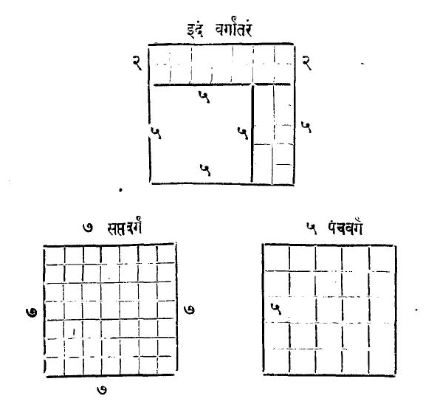
\includegraphics[scale=0.8]{Graphics/Capture5.JPG}
\end{figure}

\noindent सप्तवर्गात्पञ्चवर्गं विशोघ्य शेषमिदं वर्गांन्तरम्~। अत्र पार्श्वद्वयेऽपि क्षेत्रशेषस्य विस्तारो भुजान्तरतुल्य २ एव स्यात्~। भुजावेव ५~। ७ राशीति राश्यन्तरतुल्य २ एव विस्तारः स्यात्~। दैर्घ्यं तु एकतरपार्श्वे बृहद्भुजतुल्यम् ७ 
अन्यस्मिन् पार्श्वे लघुभुजतुल्यम् ५~।
\newpage
%%%%%%%%%%%%%%%%%%%%%%%%%%%%%%%%%%%%%%%%%%%%
\begin{figure}[h!]
    \centering
    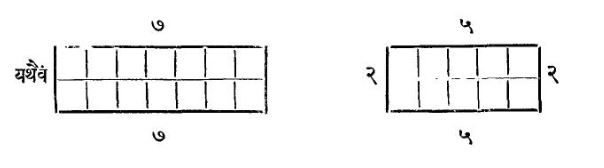
\includegraphics[scale=0.65]{Graphics/Capture6.JPG}
\end{figure}
\vspace{-2mm}

\noindent अनयोर्योगे जातं क्षेत्रशेषमेवं 

\begin{figure}[h!]
    \centering
    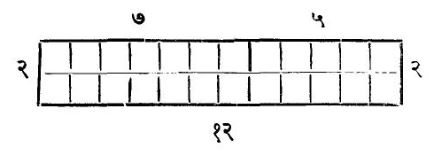
\includegraphics[scale=0.65]{Graphics/Capture7.JPG}
\end{figure}
\vspace{-2mm}

\noindent अस्य क्षेत्रस्य राशियोगतुल्यं १२ दैर्घ्यं राशन्तरतुल्यो २ विस्तारश्च~। 
आयते भुजकोटिघातः फलमिति योगान्तरघातोऽस्य फलम्~। इदं क्षेत्रशेषं हि पूर्वकल्पितराश्योर्वर्गान्तरं योगान्तरघातरूपमुपपन्नं पाद्यामुक्तं 
राश्योरन्तरवर्गेणेत्यादि~॥ द्वयोरव्यक्तयोर्यथेति~। राशी या १ का १~। 
अनयोः अन्तरवर्गः या व १ या का भा २ं काव १ अस्य 
द्विघ्नघातेनानेन या का भा २ योगे जातो वर्गयोग एव या व १ 
का व १~। अथवा तान्येव क्षेत्रखण्डान्यन्यथा 
\vspace{-3mm}

\begin{flushright}
\begin{minipage}[c]{0.3\textwidth}
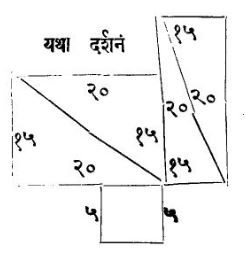
\includegraphics[scale=0.7]{Graphics/Capture8.JPG}
\end{minipage} 
\hfill
\begin{minipage}{0.55\textwidth} 
\noindent विन्यस्य क्षेत्रफलं साध्यते अत्र लघुचतुर्भुजस्य बाह्यभुजेन \;स्वमार्गवृद्धेन ~यथा \;दर्शने \;क्षेत्रं \;विछिद्य दर्शनं अतो मध्यरेखामपनीय दर्शनं एवं जातं समचतुर्भुजद्वयमेकं कोटितुल्यचतुर्भुजमपरं भुजतुल्यं~। चतुर्भुजद्वयम् अपि समकर्णम्~। अत उक्तवदेकत्र कोटिवर्गः क्षेत्रफलमपरत्र भुजवर्गं क्षेत्रफलमित्युभयोर्योगे जातो भुजकोटिवर्गयोगः प्रथमचतुर्भुजे क्षेत्रफलम्~। अस्य पदं च ७
\end{minipage} 
\end{flushright}

\newpage
%%%%%%%%%%%%%%%%%%%%%%%%%%%%%%%%%%%%%%%%%%%%%%%%%%
\begin{figure}[h!]
    \centering
    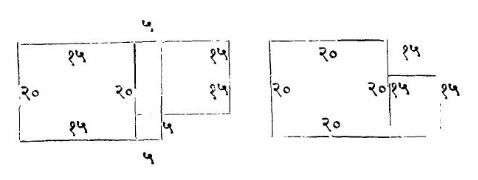
\includegraphics[scale=0.8]{Graphics/Capture9.JPG}
\end{figure}

\noindent सोधपत्रं अनङ्कपृष्ट सष्टपङ्गती दशपत्रे ६\footnote{This part is unintelligible.} \\

\vspace{-3mm}
 अथ वक्ष्यमाणोदाहरणोपयुक्तमन्यदनुष्टुब्द्वयेनाह\textendash 
\begin{quote}
    \bs
     वर्गयोगस्य यद्राश्योर्युतिवर्गस्य चान्तरम्~। \\
 द्विघ्नघातसमानं स्यात् द्वयोरव्यक्तयोर्यथा~॥~६२~॥\\

\vspace{-5mm}
 चतुर्गुणस्य घातस्य युतिवर्गस्य चान्तरम्~। \\
 राश्यन्तरकृतेस्तुल्यं द्वयोरव्यक्तयोर्यथा~॥~६३~॥
\end{quote}

अत्र प्रथमसूत्रे वर्गयोगस्य युतिवर्गस्य चान्तरे कृते द्विघ्नो घातो भवतीति
प्रतिपादितम्~। तत्र युक्तिर्द्वयोरव्यक्तयोर्यथेति~। यथा राशी या १ का १~। 
अनयोर्वर्गयोगोऽयं या व १ का व १ युतिवर्गोऽयं या व १ या का भा २ 
का व १ वर्गयोगयुतिवर्गयोरन्तरमिदं या का भा २ राश्योर्द्विघ्नघातोऽस्ति~। 
पूर्ववत् क्षेत्रद्वारा वा युक्तिः~। यथा राशी ३।५ अनयोर्वर्गौ युतिवर्गाद्वर्गद्वयं 
\begin{figure}[h!]
    \centering
    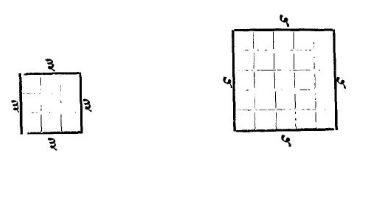
\includegraphics[scale=0.8]{Graphics/Capture10.JPG}
\end{figure}
\newpage
%%%%%%%%%%%%%%%%%%%%%%%%%%%%%%%%%%%%%%%%%%%%
\begin{figure}[h!]
    \centering
    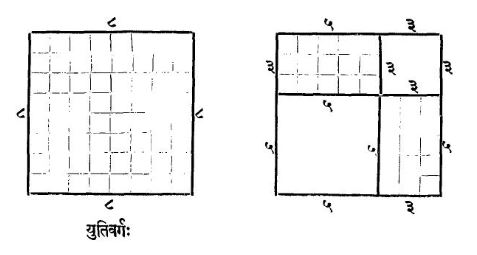
\includegraphics[scale=0.8]{Graphics/Capture11.JPG}
\end{figure}

\noindent विशोध्य शेषम्~। अत्र क्षेत्रशेषखण्डयोरेकराशितुल्यो विस्तारः~। परराशितुल्यो दैर्घ्यमिति प्रत्येकं राशिघातः फलम्~। अत उपपन्नं वर्गयोगयुतिवर्गयोरन्तरं द्विघ्नघातसममिति~॥ \\

\vspace{-3mm}
 द्वितीयसूत्रे चतुर्गुणस्य घातस्य युतिवर्गस्य चान्तरवर्गो भवतीति 
प्रतिपादितम्~। तत्र युक्तिर्द्वयोरव्यक्तयोर्यथेति~। यथा राशी या १ का १ 
अनयोर्घातश्चतुर्गुणोऽयं या का भा ४~। युतिवर्गश्चायं या व १ या का भा २ 
का व १ युतिवर्गाच्चतुर्गुणघातेऽपनीते शेषमिदं या व १ या का भा २ं 
का व १~। इदं राश्यन्तरवर्ग एव~। यद्वा क्षेत्रगतोपपत्तिः~। सा तु मूल 
एव स्फुटास्ति~॥ \\

\vspace{-3mm}
 अथोदाहरणमनुष्टुभाह\textendash 
 \begin{quote}
     \ex
     चत्वारिंशद्युतिर्येषां दोःकोटिश्रवसां वद~।\\
 भुजकोटिवधो येषु शतं विंशतिसंयुतम्~॥~७६~॥~
 \end{quote}
 
स्पष्टोऽर्थः~। अत्र किल भुजकोटिवधोऽयम् १२०~। अयं द्विघ्नः सन् २४० 
भुजकोटियुतिवर्गस्य भुजकोटिवर्गयोगस्य चान्तरं स्यात्~। वर्गयोगस्य यद्राश्यो-
\newpage
%%%%%%%%%%%%%%%%%%%%%%%%%%%%%%%%%%%%%%%%%%%%%%%%%% 
\noindent र्युतिवर्गस्य चान्तरं द्विघ्नघातसमानं स्यादित्युक्तत्वात्~। तत्र यो हि
भुजकोटिवर्गयोगः स एव पूर्वकर्णवर्गः~। अतो भुजकोटियुतिवर्गस्य कर्णवर्गस्य 
चान्तरमिदं २४० अत्र भुजकोटियुतिरेको राशिः~। अनयोर्वर्गान्तरमिदं २४० 
तच्च योगान्तरघातसममित्युक्तत्वाद्भुजकोटियुतिकर्णयोगस्य भुजकोटियुतिकर्णान्तरस्य च धातो भवति २४०~। तत्र भुजकोटियुतिकर्णयोगस्तु त्रयाणां 
योगो भवति~। स चात्र चत्वारिंशन्मित उद्दिष्ट एवास्ति ४०~। अतोऽनेन 
योगेन ४० योगान्तरघातेऽस्मिन् २४० भक्ते लब्धं भुजकोटियुतिकर्णान्तरम् ६~। 
अथ योगान्तराभ्यामेताभ्यां ४०।६ सङ्क्रमणेन जातौ राशी २३।१७~। 
भुजकोटियुतिरेकः २३~। कर्णोऽपरः १७~। अत्र लघुराशिरेव कर्णो ज्ञेयः~। 
भुजकोटियुतितस्तस्याधिक्यासम्भवात्~। उक्तमप्याचार्यै{\qt र्लीलावत्याम्}~॥ 

\begin{quote}
    \q
   धृष्टोद्दिष्टमृजुभुजं क्षेत्रं यत्रैकयाहुतः स्वल्पा~। \\
 तदितरभुजयुतिरथवा तुल्या ज्ञेयं तदक्षेत्रम्\renewcommand{\thefootnote}{*}\footnote{लीलावत्यां क्षेत्रव्यवहारे श्लोकः १६~॥}~॥~इति~॥~
\end{quote}
 
 अथ भुजकोटिवधे १२० चतुर्गुणे ४८० भुजकोटियुति\textendash \,२३\textendash \,वर्गादस्मात् ५२९ शोधिते शेषं ४९ इदं भुजकोटयन्तरवर्गः~। चतुर्गुणस्य घातस्य युतिवर्गस्य चान्तरं राश्यन्तरकृतेः तुल्यमित्युक्तत्वात्~। अतोऽस्य ४९ मूलं ७ भुजकोट्योरन्तरम्~। भुजकोटियोगश्चायम् २३ आभ्यां सङ्क्रमणेन जाते भुजकोटी ८।१५~॥ \\

\vspace{-3mm}
 अथान्यदुदाहरणमनुष्टुभाह\textendash 
\begin{quote}
    \ex
      योगो दोःकोटिकर्णानां षट्पञ्चाशत् ५६ वधस्तथा~। \\
 षट्शताः सप्तभिः क्षुण्णा ४२०० येषां तान्मे पृथग्वद~॥~७७~॥~
\end{quote}

स्पष्टोऽर्थः~। अत्र कर्णं यावत्तावन्मितं प्रकल्प्य गणितमाकरे स्फुटम्~॥ 
\newpage
%%%%%%%%%%%%%%%%%%%%%%%%%%%%%%%%%%%%%%%%%%%
 
\begin{quote}
    \qt
 दैवज्ञवर्यगणसन्ततसेव्यपार्श्व-\\

\vspace{-7mm}
\hspace{1cm} बल्लालसञ्ज्ञगणकात्मजनिर्मितेऽस्मिन्~। \\

\vspace{-7mm}
 बीजक्रियाविवृतिकल्पलतावतारेऽभूत् \\

\vspace{-7mm}
\hspace{1cm} एकवर्णजसमीकरणं सभेदम्~॥~८~॥~
\end{quote}

\begin{center}
 इति श्रीसकलगणकसार्वभौमश्रीबल्लालदैवज्ञसुतश्रीकृष्णगणकविरचिते \\
 बीजविवृतिकल्पलतावतारे निजभेदमध्यमाहरणसहितमेकवर्णसमीकरणम्~॥ 
\end{center}

 अत्र खण्डयोर्ग्रन्थसङ्ख्ये ४९०।३२५ एवमेकवर्णसमीकरणे ग्रन्थसङ्ख्या
८१५ एवमादितो जातग्रन्थसङ्ख्या ३३९५~॥
\begin{figure}[h!]
    \centering
    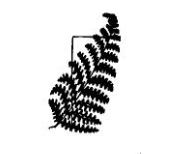
\includegraphics[scale=0.7]{Graphics/Capture.JPG}
\end{figure}
\newpage
%%%%%%%%%%%%%%%%%%%%%%%%%%%%%%%%%%%%%%%%%%%%%%%
\phantomsection \label{anekavarna}
\begin{center}
    \textbf{\LARGE  अथ अनेकवर्णसमीकरणम्}
\end{center}
\thispagestyle{empty}

 \vspace{2mm}
 श्रीः~। एवमनेकवर्णानामेकवर्णपूर्वकत्वादादावेकवर्णसमीकरणमुक्त्वेदानीं क्रमप्राप्तम् अनेकवर्णसमीकरणं शालिन्योपजातिकाद्वयेन शालिनीपूर्वार्धेन चाह\textendash
\begin{quote}
    \bs
      आद्यं वर्णं शोधयेदन्यपक्षात् \\

\vspace{-7mm}
\hspace{0.5cm} अन्यान् रूपाण्यन्यतश्चाद्यभक्ते~। \\

\vspace{-7mm}
 पक्षेऽन्यस्मिन्नाद्यवर्णोन्मितः स्यात् \\

\vspace{-7mm}
\hspace{0.5cm} वर्णस्यैकस्योन्मितीनां बहुत्वे~॥~६४~॥~\\

 \vspace{-5mm}
 समीकृतच्छेदगमे तु ताभ्यस्तदन्यवर्णोन्मितयः प्रसाध्याः~। \\

\vspace{-7mm}
 अन्त्योन्मितौ कुट्टविधेर्गुणाप्ती ते भाज्यतद्माजकवर्णमाने~॥~६५~॥~\\

\vspace{-5mm}
 अन्येऽपि भाज्ये यदि सन्ति वर्णाः \\

\vspace{-7mm}
\hspace{0.5cm} तन्मानमिष्टं परिकल्प्य साध्ये~। \\

\vspace{-7mm}
 विलोमकोत्थापनतोऽन्यवर्ण- \\

\vspace{-7mm}
\hspace{0.5cm} मानानि भिन्नं यदि मानमेवम्~॥~६६~॥~\\

\vspace{-5mm}
 भूयः कार्यः कुट्टकोऽत्रान्त्यवर्णं \\

\vspace{-7mm}
\hspace{0.5cm} तेनोत्थापयेद्व्यस्तमाद्यान्~॥ 
\end{quote}

अस्मिन् शालिनीपूर्वार्धेऽन्यपाठद्वयं दृश्यते~। 
\begin{quote}
     {\bs "भूयः कार्यः कुट्टकादन्य वर्णः"} इति~। \\
     
     \vspace{-5mm}
 {\bs "भूयः कार्यः कुट्टकादन्यवर्णस्तेनो- \\

\vspace{-7mm}
\hspace{2mm} त्थाप्योत्थापयेदन्तिमाद्यान्~॥"} \textbf{इति च~॥~}
\end{quote}

एतानि सूत्राणि आचार्यैरेव सम्यग्व्याख्यातानीति नास्माभिर्व्याक्रियन्ते~।
अथ शालिनीपूर्वार्धं व्याख्याय उत्थापने कृतेऽन्यवर्णमानं भिन्नं लभ्यते 
तदात्र भूयः कुट्टकः कार्यः~। तेन कुट्टकेन अन्त्यर्णमुत्थाप्य आद्यात्
\afterpage{\fancyhead[RE]{\textbf{बीजपल्लवे}}}
\afterpage{\fancyhead[LO]{\textbf{अनेकवर्णसमीकरणम्}}}
\afterpage{\fancyhead[RO,LE]{\textbf{\thepage}}}
\cfoot{}
\newpage
%%%%%%%%%%%%%%%%%%%%%%%%%%%%%%%%%%%%%%%%%%%%%%%%%%%%%%%%

\noindent व्यस्तमुत्थापयेत्~। कुट्टको गुणविशेष इति प्रागेव निरूपितम्~। तेन 
कुट्टकेन सक्षेपेण गुणेन अन्त्ययोरन्त्येषु वा वर्णमानेषु यो वर्णस्तम् उत्थाप्य 
आद्याद्व्यस्तं पुनरुत्थापयेत्~। यस्योन्मानस्य पूर्वमुत्थापने भिन्नं मानमभवत्तदुन्मानमाद्यं तत आरभ्य पुनरपि विलोमोत्थापनं कर्तव्यमित्यर्थः~। अयमेव पाठो
मुख्यः~। आचार्यैः सूत्रविवरणावसरेऽस्यैव विवरणात्~। तद्विवरणं यथा~।
अथ यदि विलोमोत्थापने क्रियमाणे पूर्ववर्णोन्मितौ तन्मितिर्भिन्ना लभ्यते तदा कुट्टकविधिना यो गुणः सक्षेप उत्पद्यते स भाज्यवर्णस्य मानं
तेनान्त्यवर्णमानेषु तं वर्णमुत्थाप्य पूर्वोन्मितिषु विलोमोत्थापनप्रकारेण अन्यवर्णमानानीति भूयः कार्यः कुट्टकादन्त्यवर्ण इति पाठ एव साधु~। उत्थाप्येतिपदस्य
अनन्वयात्~। अत्र यद्यपि आद्यम् इत्यध्याहृत्य आद्यमुत्थाप्येति तदन्वयः स्यात्तथापि 
अन्त्यवर्णोत्थापनस्यानुक्ते न्यूनतादोषः स्यादेव~। यदि न्यूनतादोषपरिहारार्थमन्त्यवर्णमित्यध्याह्रियेत तथा सति तेन अन्त्यवर्णेन
अन्त्यवर्णमुत्थाप्येति तदन्वयः स्यात्~। इह हि यदि अन्यवर्णमानं भिन्नं स्यात्तदा भूयः 
कुट्टकात् अन्यवर्णः कार्य इत्युक्तेरन्यवर्णो भाजकवर्ण एव~। एवं सति 
भाजकवर्णमानेन अन्त्यवर्णम् उत्थाप्येत्यर्थः पर्यवस्यति~। न चासौ युक्तः~। 
भाजकवर्णान्त्यवर्णयोर्भेदात्~। किन्तु भाज्यवर्णस्यान्त्यवर्णस्य
चाभेदाद्भाज्यवर्णमानेनैवान्त्यवर्णोत्थापनं युक्तम्~। तदेवं द्वितीयपाठो न साधुः~। एवं
तृतीयपाठोऽप्यसाधुः~। \\

\vspace{-3mm}
 अथैतस्यार्थस्य स्पष्टत्वार्थं वक्ष्यमाणमुदाहरणं लिख्यते~॥ 
\begin{quote}
\hyperref[Ex 81]{"षड्भक्तः पञ्चाग्रः पञ्चविभक्तो भवेच्चतुष्काग्रः~। \\
चतुरुद्धृतस्त्रिकाग्रो द्वयग्रस्त्रिसमुद्धृतकः स्यात्~॥"} इति
\end{quote}
 
 अत्र राशिः या १ अयं षड्भक्तः पञ्चाग्र इति लब्धिप्रमाणं 
कालकं प्रकल्प्य कालकगुणितो हरः स्वाग्रेण पञ्चकेन युतो का ६ रू ५ यावत्तावत्सम इति साम्यकरणेन जाता यावत्तावदुन्मितिः $\begin{matrix}
\vspace{-1mm}
\mbox{का ६}\\
\vspace{-1.5mm}
\mbox{या १}
\vspace{1mm}
\end{matrix}$ रू ५ एवं पञ्चादिहरेषु नीलकादयो लभ्यन्त इति जाता
\newpage
 %%%%%%%%%%%%%%%%%%%%%%%%%%%%%%%%%%%%%%%%%%%%%%%%%% 

\noindent यावत्तावदुन्मितयः नी ५ $\begin{matrix}
\vspace{-1mm}
\mbox{रू ४}\\
\vspace{-1.5mm}
\mbox{या १}
\vspace{1mm}
\end{matrix}$~। $\begin{matrix}
\vspace{-1mm}
\mbox{पी ४}\\
\vspace{-1.5mm}
\mbox{या १}
\vspace{1mm}
\end{matrix}$ रू ३~। $\begin{matrix}
\vspace{-1mm}
\mbox{लो ३}\\
\vspace{-1.5mm}
\mbox{या १}
\vspace{1mm}
\end{matrix}$ रू २~। आसां प्रथमद्वितीययोः समीकरणेन लब्धा कालकोन्मितिः $\begin{matrix}
\vspace{-1mm}
\mbox{नी ५}\\
\vspace{-1.5mm}
\mbox{का ६}
\vspace{1mm}
\end{matrix}$ रू १ं द्वितीयतृतीययोर्नीलकोन्मितिः $\begin{matrix}
\vspace{-1mm}
\mbox{नी ४}\\
\vspace{-1.5mm}
\mbox{पी ५}
\vspace{1mm}
\end{matrix}$ रू १ं एवं तृतीयचतुर्थ्योः पीतकोन्मितिः 
$\begin{matrix}
\vspace{-1mm}
\mbox{लो ३}\\
\vspace{-1.5mm}
\mbox{पी ४}
\vspace{1mm}
\end{matrix}$ रू १ं~। इयमन्त्या~। अन्त्योन्मितौ कुट्टविधेर्गुणाप्ती इत्यादिना जाते लोहितपीतकयोर्माने सक्षेपे $\begin{matrix}
\vspace{-1mm}
\mbox{ह ३ रू २ पी}\\
\vspace{-1.5mm}
\mbox{ह ४ रू ३ लो}
\vspace{1mm}
\end{matrix}$ अथ नीलकोन्मानमिदम्~। पी ४ $\begin{matrix}
\vspace{-1mm}
\mbox{रू १ं}\\
\vspace{-1.5mm}
\mbox{नी ५}
\vspace{1mm}
\end{matrix}$ अत्र नीलकपञ्चकस्य रूपोनं पीतकचतुष्टयं मानमस्ति~॥ 
तत्र पीतकस्य कुट्टकसिद्धं मानमिदम्~। ह ३ रू २ अतो यद्येकस्य 
पीतकस्येदं मानं तदा पीतकचतुष्टयस्य किमिति पी १~। ह ३ रू २~। पी ४ 
त्रैराशिकेन जातं पीतकचतुष्टयस्य मानं ह १२ रू ८ इदं रूपोनं जातं 
नीलकपञ्चकस्य मानं ह १२ रू ७~। यदि नीलकपञ्चकस्येदं तदैकस्य 
नीलकस्य किमिति नी ५~। ह १२ रू ७~। नी १ त्रैराशिकेन नीलकस्य 
मानं भिन्नं लभ्यते \framebox[1.4\width]{ह $\begin{matrix}
\vspace{-1.5mm}
\mbox{११}\\
\vspace{-1.5mm}
\mbox{५}
\vspace{1mm}
\end{matrix}$ रू ७} अतोऽत्र भूयः कुट्टककार्यः 
कुट्टको गुणकविशेषः स चोक्तविधिना जातः सक्षेपः श्वे ५ रू ४~। गुणाप्ती 
ते भाज्यतद्भाजकवर्णमाने इत्युक्तत्वादसौ कुट्टको श्वे ५ रूप ४ भाज्यवर्णस्य 
हरितकस्य मानं श्वे ५ रू ४ ह~। अनेनान्त्ययोः पीतकलोहितकमानयोरनयोः 
$\begin{matrix}
\vspace{-1mm}
\mbox{ह ३ रू २}\\
\vspace{-1.5mm}
\mbox{ह ४ रू ४}
\vspace{1mm}
\end{matrix}$~। पीतवर्णं हरितकमुत्थाप्य आद्याद्व्यस्तं पुनरुत्थापनं 
यथा~। इह हरितकत्रयं रूपद्वययुतमेकस्य पीतकस्य मानमस्ति~। हरितकमानं 
च कुट्टकसिद्धमिदं श्वे ५ रू ४ यद्येकस्य हरितकस्येदं मानं तर्हि
\newpage
 %%%%%%%%%%%%%%%%%%%%%%%%%%%%%%%%%%%%%%%%%%%%%%%%%% 

\noindent हरितकत्रयस्य किमिति ह १~। श्वे ५ रू ४~। ह ३~। त्रैराशिकेन जातं हरितकत्रयमानं श्वे १५ रू १२~। इदं रूपद्वययुतं जातं पीतकमानं 
श्वे १५ रू १४~। पी १~। अनयैव युक्त्या लोहितकमानमपि~। श्वे २० 
रू २०~। लो १~। एवं जाते लोहितकपीतकयोर्माने श्वे २० रू २०~। 
श्वे १५ रू १४~। एवं जातं कुट्टकेनान्त्यवर्णोत्थापनम्~॥ \\

\vspace{-3mm}
 अथ लोहितपीतकयोराद्यान्नीलकादारभ्य व्यस्तमुत्थापयेत्~। तत्र 
नीलकमानमिदं पी ४ रू १ं इह रूपोनं पीतकचतुष्टयं नीलकपञ्चकस्य 
मानमस्ति~। तत्र पीतकमानमिदम्~। श्वे १५ रू १४~। पी १~। यद्येकस्य 
पीतकस्येदं तदा पीतकचतुष्टयस्य किमिति पी १~। श्वे १५ रू १४~। पी ४~। 
त्रैराशिकेन पीतकचतुष्टयमानं श्वे ६० रू ५६ इदं रूपोनं सत् जातं 
नीलकपञ्चकस्य मानं श्वे ६० रू ५५~। यदि नीलकस्य पञ्चकस्येदं तदैकस्य 
नीलकस्य किमिति~। नी ५~। श्वे ६० रू ५५~। नी १~। त्रैराशिकेन 
जातं नीलकमानं श्वे १२ रू ११~। नी १~। अथ नीलकाद्यः कालकस्तस्य 
मानमिदं $\begin{matrix}
\vspace{-1mm}
\mbox{{नी ५ रू १ं}}\\
\vspace{-1.5mm}
\mbox{{क ६}}
\vspace{1mm}
\end{matrix}$~। इह रूपोनं नीलकपञ्चकं कालकषट्कस्य 
मानमस्ति~। प्राग्वत् त्रैराशिकेन जातं नीलकपञ्चमानं श्वे ६० रू ५५ 
इदं रूपोनं सज्जातं कालकषट्कमानं श्वे ६० रू ५४~। अतोऽनुपाताज्जातमेकस्य कालकस्य मानं श्वे १० रू ९~। का १~। अथ कालकादाद्यो 
यावत्तावत्~। तस्य मानमिदम् $\begin{matrix}
\vspace{-1mm}
\mbox{{का ६ रू ५}}\\
\vspace{-1.5mm}
\mbox{{या १}}
\vspace{1mm}
\end{matrix}$~। इह कालकषट्करूपपञ्चकयुतं 
यावत्तावतो मानमस्ति~। तत्र कालकषट्कस्य सिद्धमानमिदं श्वे ६० रू ५४~। 
इदं रूपपञ्चकयुतं जातं यावत्तावन्मानं श्वे ६० रू ५९~। या १~। एवमन्यास्वपि 
यावत्तावदुन्मितिषु उत्थापनेनेदमेव मानं सिद्ध्यति~। तदेवं जातानि 
यावत्तावदादीनां मानानि व्यक्ताव्यक्तानि $\begin{matrix}
\mbox{श्वे ६० रू ५९~। या १~।}\\
\mbox{श्वे १० रू ~९~। का १~।}\\
\mbox{श्वे १२ रू ११~। नी १~।}\\
\mbox{श्वे १५ रू १४~। पी १~।}\\
\mbox{श्वे २० रू १९~। लो १~।}\\
\end{matrix}$ अत्र श्वेत- 

\newpage%%%%%%%%%%%%%%%%%%%%%%%%%%%%%%%%%%%%%%%%%%%%%%%%%% 
\noindent कस्य शून्ये माने कल्पिते जातो राशिः ५९~। कालकादयस्तु षडादि 
भाजकानां लब्धयः कल्पिताः~। अतस्तन्मानानि जाताः क्रमाल्लब्धयः~। 
५९~। ११~। १४~। १९~। एवं श्वेतकस्य मानं रूपमिष्टं १ प्रकल्प्य 
जातो राशिः ११९ लब्धयश्च १९~। २३~। २९~। ३९~। एवमिष्टवशादानन्त्यम्॥ \\

\vspace{-3mm}
 अथोपपत्तिः उच्यते~॥ अत्र किल बहूनां मानान्यव्यक्तानि सन्ति~। तत्र 
पूर्वयुक्त्या एकस्मिन् पक्षे यद्येकम् एवाव्यक्तं स्यादन्यत्र च रूपाण्येव
स्युस्तदा तस्याव्यक्तस्य मानं सुबोधम्~। अतस्तथा यतितव्यं यथैकस्मिन् पक्षे 
एकमेवाव्यक्तं स्यात्समत्वाविरोधेन~। तत्र \hyperref[Ex 78]{"अश्वाः पञ्चगुणाङ्गमङ्गलमिता"} इति वक्ष्यमाणमुदाहरणमधिकृत्य युक्तिरुच्यते~। अत्रा-श्वादीनां मूलान्यज्ञातानीति यावत्तावदादीनि कल्पितानि या १~। का १~। नी १~। पी १~। अतोऽनुपातेन निजाश्वादीनां धनान्येकीकृत्य जातानि चतुर्णां समधनानि~।
$\begin{matrix}
\mbox{या ५ का २ नी ८ पी ७~।}\\
\mbox{या ३ का ७ नी २ पी १~।}\\
\mbox{या ६ का ४ नी १ पी २~।}\\
\mbox{या ८ का १ नी ३ पी १~।}\\
\end{matrix}$ अत्र चतुर्णामपि धनानि समानीति प्रथमद्वितीयधने अपि सम एव~। $\begin{matrix}
\vspace{-1mm}
\mbox{या ५ का २ नी ८ पी ७}\\
\vspace{-1.5mm}
\mbox{या ३ का ७ नी २ पी १}
\vspace{1mm}
\end{matrix}$ अत्रैकपक्षे यथैकमेवाव्यक्तं भवति तथा यतितव्यम् तत्रैकतरपक्षे एकं वर्णं विहाय यदवशिष्यते तत्तुल्यं चेदुभयोः पक्षयोः शोध्यते तर्ह्येकस्मिन्पक्षे
एकमेवाव्यक्तं स्यात्~। यं विहायावशिष्टं शोध्यते तस्मिन्पक्षे तस्यैव
वर्णस्य शेषत्वात्~। तत्र कं वर्णमपहाय शेषं पक्षयोः शोध्यमिति यद्यपि नास्ति 
नियमस्तथापि प्रथमातिक्रमे कारणाभावात्प्रथमवर्णमपहायशेषं पक्षयोः शोध्यम्~। 
अथ प्रकृते प्रथमवर्णमपहाय शेषमिदम्~। का २ नी ८ पी ७~। 
अस्मिन्पक्षयोः शोधिते जातमाद्यपक्षे या ५ द्वितीयपक्षे तु जातं या ३ 
का ५ नी $\dot{\text{६}}$ पी $\dot{\text{६}}$~। अस्ति चानयोस्समत्वम्~। समयोः समक्षेपे

\newpage
 %%%%%%%%%%%%%%%%%%%%%%%%%%%%%%%%%%%%%%%%%%%%%%%%%% 

\noindent समशुद्धौ वा समत्वाहानेः तथा सति यदेव यावत्तावत्पञ्चकस्य मानं तदेव नीलकषट्क-पीतकषट्करहितस्य यावत्त्रयकालकपञ्चकयोगस्यापीति सिद्धम्~। तथाच यावत्पञ्चकस्य मानं यावत्त्रयस्यापि ज्ञानमपेक्षितम्~। तत्र यदि स्वमानज्ञाने
स्वमानज्ञानापेक्षा स्यात्तदात्माश्रयात्कल्पकोटिशतैरपि मानज्ञानं न स्यात्~। अतः सा यथा न भवति तथा यतितव्यम्~। इतरपक्षे यः सजातीयो वर्णस्तत्तुल्यं पक्षयोः 
शोध्यम्~। प्रकृते इतरपक्षे सजातीयो वर्णोऽयम्~। या ३~। एतस्मिन्पक्षयोः 
शोधितजातमाद्यपक्षे~। या २~। द्वितीयपक्षे~। का ५ नी ६ं पी ६ं~। एवं कृते 
यदेव यावत्तावद्द्वयस्य मानं तदेव नीलकषट्कपीतकषट्करहितस्य कालकपञ्चकस्य मानमिति नास्ति स्वमानज्ञानापेक्षा~। अत उक्तम् आद्यं वर्णं शोधयेदन्य-पक्षादन्यान् रूपाण्यन्यतश्चेति~॥ \\

\vspace{-3mm}
 अथातस्त्रैराशिकम्~। यदि यावत्तावद्द्वयस्येदं मानं तदेकस्य यावत्तावतः 
किम् इति~। या २~। का ५ नी ६ं पी ६ं~। या १ त्रैराशिकेन जातं 
यावत्तावदुन्मानं का ५ नी ६ं $\begin{matrix}
\vspace{-1mm}
\mbox{पी ६ं}\\
\vspace{-1.5mm}
\mbox{या २}
\vspace{1mm}
\end{matrix}$ अत्र हरे याकारलिखनं यावत्तावन्मानमिदमित्युपस्थित्यर्थं न तु यावत्तावद्द्वयहरः प्रमाणेच्छयोर्यावत्तावतापवर्तनात्~। अनपवर्ते तु इच्छया गुणने क्रियमाणे भावितं स्यात्~। तदेवमुक्तप्रकारेण प्रथमद्वितीययोर्द्वितीयतृतीययोस्तृतीयचतुर्थयोश्च धनयोः
समशोधनेन जाताः प्रथमवर्णोन्मितयः का ५ नी ६ं $\begin{matrix}
\vspace{-1mm}
\mbox{पी ६ं}\\
\vspace{-1.5mm}
\mbox{या २}
\vspace{1mm}
\end{matrix}$~। का ३ नी १ $\begin{matrix}
\vspace{-1mm}
\mbox{पी १ं}\\
\vspace{-1.5mm}
\mbox{या ३}
\vspace{1mm}
\end{matrix}$~। का ३ नी २ं $\begin{matrix}
\vspace{-1mm}
\mbox{पी १}\\
\vspace{-1.5mm}
\mbox{या २}
\vspace{1mm}
\end{matrix}$~। तदेतदुक्तम् आद्यभक्ते पक्षे अन्यस्मिन्नाद्यवर्णोन्मितिः 
स्यादिति~। एवं प्रथमतृतीययोः प्रथमचतुर्थयोर्द्वितीयचतुर्थयोश्च समशोधनेन
अन्या अपि यावत्तावदुन्मितयः सम्भवन्ति परं प्रयोजनाभावान्न कृताः॥ \\

\vspace{-3mm}
 अथ भाज्यवर्णानां कालकादीनामिष्टानि मानानि प्रकल्प्य ऐक्यं 
कृत्वा यदि स्वहरेण ह्रियते तदा भिन्नमभिन्नं वा प्रथमवर्णमानं स्यात्~।
 \newpage%%%%%%%%%%%%%%%%%%%%%%%%%%%%%%%%%%%%%%%%%%%%%%%%%% 
\noindent इतरेषां तु कल्पितान्येव~। तथा सति सुखेनोद्दिष्टसिद्धिः~। अथ
यद्यभिन्नमेव मानमपेक्षितं तर्हि यं कञ्चिदेकं वर्णं विहाय परेषां मानानीष्टानि 
कल्प्यानि~। तथा सति भाज्ये एको वर्णः कानिचित् रूपाणि च स्युः~। 
अथ तस्य वर्णस्य मानं तथेष्टं कल्प्य यथा तेनेष्टेन गुणितो वर्णाङ्कस्तै 
रूपैर्युतो हरभक्तो निःशेषः स्यात्~। एवं कृते प्रथमवर्णमानमभिन्नमेव स्यात्~। \\

\vspace{-3mm}
 अथ तादृशस्येष्टस्य ज्ञानार्थमुपायः~। इह हि वर्णाङ्कः केन गुणितस्तै 
रूपैर्युतः स्वहरहृतो निश्शेषः स्यादिति विचारः कुट्टके पर्यवस्यति~। अथ 
कुट्टकविधिना यो गुणः स्यात्तेन गुणितो वर्णाङ्कस्तै रूपैर्युतः स्वहरभक्तो
निःशेषः स्यादेवेति भाज्यवर्णस्य गुणतुल्ये माने कल्पिते भाजकवर्णस्य मानं
लब्धितुल्यमभिन्नमेव स्यात्~। अत उक्तं कुट्टविधेर्गुणाप्ती ते भाज्यतद्भाजकवर्णमाने 
अन्येऽपि भाज्ये यदि सन्ति वर्णास्तन्मानमिष्टं परिकल्प साध्ये इति~। अत्र 
भाज्यवर्णमानानां यदीष्टकल्पनमुक्तं तत्तेषां मानेऽनियते सत्येव ज्ञेयम्~। यदि तु 
केनापि प्रकारेण तन्मानं नियतं सिद्ध्येत्तदा नियतेष्टकल्पनेन व्यभिचार एव
स्यात् यथास्मिन्नेवोदाहरणे यथा चतुर्णां समधनत्वमुद्दिष्टं तथा यदि द्वयोरेव 
या ५ का २ नी ८ पी ७ या ३ का ७ नी २ पी २ उद्दिष्टं स्यात्तदा 
तदुत्पन्नोन्मितौ $\begin{matrix}
\vspace{-1mm}
\mbox{का ५}\\
\vspace{-1.5mm}
\mbox{या २}
\vspace{1mm}
\end{matrix}$ नी ६ं पी ६ं भाज्यवर्णमानानामनियतत्वात्तदिष्टकल्पनेन 
उद्दिष्टसिद्धिः स्यात्~। यथात्र कालकादीनाम् इष्टानि कल्पितानि ४~। १~। २ 
एभ्यो जातं यावत्तावन्मानं १ जातान्यश्वादिमूल्यानि~। १~। ४~। १~। २ 
यद्वा कल्पितानि ६~। २~। १ जातं यावत्तावन्मानं ६ जातान्यश्वादिमूलानि 
६~। ६~। २~। १~। यद्वा कल्पितानि~। ६~। १~। २ जातानि 
मूल्यानि ६~। ६~। १~। २ यद्वा कल्पितानि~। ४~। १~। १ जातानि 
मूल्यानि ४~। ४~। १~। १ एवमिष्टवशादनेकधा~। यदि त्वनयोर्धनयोरन्यधनेनापि समतोद्दिष्टा स्यात्तदा भाज्यवर्णमानानामिष्टकल्पने व्यभिचारः स्यादेव 
नह्यन्यधनानुरोधेन काचित् क्रियात्र कृतास्ति येनान्यधनसमता सिद्ध्येत~। 
यदि तु तदनुरोधिक्रियां विनापि तत्समता सिद्ध्येत्तदा किमीदृग्धनं
\newpage
%%%%%%%%%%%%%%%%%%%%%%%%%%%%%%%%%%%%%%%%%%%%%%%%%

\noindent स्याद्यत्समं न स्यात्~। तस्मादेतादृश्युदाहरणे भाज्यवर्णमानानामिष्टकल्पनं न युक्तं किन्तु नियतमेव तन्मानं साध्यम्~। तच्च यथा समपक्षेभ्य आद्यवर्णमानं साधितं तथा भाज्याद्य-वर्णस्यापि साध्यम्~। अथ उक्तं 
वर्णस्यैकस्योन्मितीनां बहुत्वे समीकृतछेदगमे तु ताभ्यः तदन्यवर्णोन्मितयः
प्रसाध्या इति~। अत्र बहुत्वमनेकत्वम्~। उन्मितिद्वयादप्यन्यवर्णोन्मितिः
सम्भवात्~। समीकृतछेदगम इत्यत्रोपपत्तिस्तु एकवर्णसमीकरणे आचार्येणैव 
स्पष्टीकृता~। अथ प्रकृतोदाहरणे यावत्तावदुन्मितयः का ५ नी ६ं 
$\begin{matrix}
\vspace{-1mm}
\mbox{पी ६ं}\\
\vspace{-1.5mm}
\mbox{या २}
\vspace{1mm}
\end{matrix}$~। का ३ $\begin{matrix}
\vspace{-1mm}
\mbox{नी १}\\
\vspace{-1.5mm}
\mbox{या ३}
\vspace{1mm}
\end{matrix}$ पी १ं~। का ३ नी २ं $\begin{matrix}
\vspace{-1mm}
\mbox{पी १}\\
\vspace{-1.5mm}
\mbox{या २}
\vspace{1mm}
\end{matrix}$~। अत्र हरे याकारस्यावास्तवत्वादन्योन्यहाराभिहतौ हरांशावित्यादिना भावितं न भवति~। याकारस्य वास्तवत्वेऽपि हाराभ्यामपवर्तिताभ्यां यद्वा हरांशौ गुण्यावित्युक्तत्वाद्धरयोर्यावत्तावतपवर्तनाद्भावितं न भवति~। अत्र प्रथमद्वितीययोर्द्वितीयतृतीययोः प्रथमतृतीययोश्च जाताः कालकोन्मितयः~। नी २०
$\begin{matrix}
\vspace{-1mm}
\mbox{पी १६}\\
\vspace{-1.5mm}
\mbox{का ९}
\vspace{1mm}
\end{matrix}$~। नी ८ $\begin{matrix}
\vspace{-1mm}
\mbox{पी ५ं}\\
\vspace{-1.5mm}
\mbox{का ३}
\vspace{1mm}
\end{matrix}$~। नी ४ $\begin{matrix}
\vspace{-1mm}
\mbox{पी ७}\\
\vspace{-1.5mm}
\mbox{का २}
\vspace{1mm}
\end{matrix}$~। अत्राप्येकतरस्येष्टं मानं प्रकल्प्य परस्य तथेष्टं कल्प्यं यथा 
कालकमानमभिन्नं भवेत्~। परं भाज्यवर्णमाननियतत्वे तदिष्टकल्पनमयुक्तम्~।
भवति चात्र कालकोन्मितिभ्यां समीकृतछेदाभ्यां छेदगमादिना नीलकोन्मानं नियतम्~।
$\begin{matrix}
\vspace{-1mm}
\mbox{पी ३१}\\
\vspace{-1.5mm}
\mbox{नी ४}
\vspace{1mm}
\end{matrix}$~। अत्र यदेव एकत्रिंशत्पीतकमानं तदेव नीलकचतुष्टयस्य~। 
अत्राप्यभिन्नत्वार्थं पीतकस्य तथेष्टं मानं कल्प्यं यथा तद्गुणितः
पीतकाङ्कश्चतुर्भिर्भक्तः शुद्ध्येत्~। अस्ति चायं कुट्टकविषयः~। अत्र भाज्यवर्णाङ्को
भाज्यः भाजकवर्णाङ्को भाजकः यत्र तु भाज्ये रूपाण्यपि स्युः तत्र रूपाणि 
क्षेपः~। इह तु~पीतकाङ्कः केन गुणितः चतुर्भक्तः शुद्ध्येदित्येवास्तीति क्षेपाभावः~॥
\newpage
%%%%%%%%%%%%%%%%%%%%%%%%%%%%%%%%%%%%%%%%%%%%%%%%%% 
 अथ कुट्टकार्थं न्यासः~। $\begin{matrix}
\vspace{-1mm}
 \mbox{भा ३९}\\
\vspace{-1.5mm}
 \mbox{रू ४}
\vspace{1mm}
 \end{matrix}$ क्षे ०~। क्षेपाभावोऽथवा यत्र क्षेपः शुद्ध्येद्धरोद्धतः ज्ञेयः शून्यं गुणं तत्र क्षेपो हरहृतः फलमिति जातौ लब्धिगुणौ $\begin{matrix}
\vspace{-1mm}
\mbox{ल ०}\\
\vspace{-1.5mm}
\mbox{गु ०}
\vspace{1mm}
\end{matrix}$~। अत्र इष्टाहतस्वस्वहरेण युक्ते ते वा 
भवेतां बहुधा गुणाप्ती इत्युक्तत्वादिष्टगुणा एकत्रिंशल्लब्धौ क्षेप्याः इष्टगुणाश्चत्वारो गुणे क्षेप्याः~। तत्रेष्टस्य इच्छाधीनत्वेनानियतत्वाद्वर्णस्वरूपमिष्टं 
प्रकल्पनीयम्~। वर्णस्य हि यद्यन्मानं कल्प्यते तत्तत्सम्भवतीति सर्वेष्टानामनुगमः 
स्यात्~। यदि तु व्यक्तमिष्टं कल्प्यते तदा न सर्वेष्टसिद्धिः~॥\\

\vspace{-3mm}
 अथ प्रकृते यावत्तावदादीनां पीतकपर्यन्तानां मानानि नियतानि 
सन्तीति तेषामन्यतमस्येष्टकल्पने सर्वेष्टानुगमो न स्यादत एभ्योऽन्यो वर्ण इष्टः 
कल्पितः लो १ अनेन गुणिते स्वस्वहरे क्षिप्ते सति जातौ लब्धिगुणौ~। लो ३१ रू ० ल~। अत्र पीतकाङ्को येन गुणितः स्वहरभक्तो 
निश्शेषः स्यात्स गुण एव पीतकस्येष्टं लो ४ रू ० गुणमानं स्यात् 
यल्लभ्यते तदेव नीलकमानमभिन्नं स्यादिति गुणो भाज्यवर्णमानं लब्धिस्तु 
भाजकवर्णमानमिति~। तथा सति जाते नीलकपीतकयोर्माने $\begin{matrix}
\vspace{-1mm}
\mbox{लो ३१ रू ० नी}\\
\vspace{-1.5mm}
\mbox{लो ४ ~रू ० पी}
\vspace{1mm}
\end{matrix}$ तदेवमन्त्योन्मितौ भाज्यवर्णमानं नियतं नास्तीति तस्य मानमिष्टं कल्प्यम्~। तत्रापि कुट्टकसिद्धगुणतुल्ये इष्टे कल्पिते भाजकवर्णमानम् अभिन्नं
भवतीति गुणतुल्यं भाज्यं वर्णमानं कल्प्यते~। पूर्वोन्मितिषु तु भाज्यवर्णमानानां नियतत्वादिष्टकल्पनमयुक्तम्~। अत उक्तमन्त्योन्मितौ कुट्टविधेरित्यादि~। 
अथ पूर्वपूर्ववर्णोन्मितिषु उत्तरोत्तरवर्णभाज्यतया तिष्टन्तीति उत्तरोत्तरवर्णमानज्ञानं विना पूर्वपूर्ववर्णमानं न सिद्ध्येदत उक्तं विलोमकोत्थापनतोऽन्यवर्णमानानीति~। अथ प्रकृते कालकोन्मितिरियम्~। $\begin{matrix}
\vspace{-1mm}
 \mbox{नी २० पी १६}\\
\vspace{-1.5mm}
 \mbox{~~~~~~ का ९}
\vspace{1mm}
 \end{matrix}$~। अत्र
\newpage
%%%%%%%%%%%%%%%%%%%%%%%%%%%%%%%%%%%%%%%%%%%%%%%%%%%

\noindent विंशतिनीलकषोडशपीतकयोगो नवभक्तः कालकमानमस्ति~। तत्र यद्येकस्य नीलकस्येदं मानं तदा विंशतिनीलकानां किमिति~। नी १~। लो ३१ 
रू ०~। नी २०~। त्रैराशिकेन जातं नीलकविंशतेर्मानं लो ६२० 
रू ०~। अथैकस्य पीतकस्येदं तदा षोडशपीतकानां किमिति~। पी १~। 
लो ४ रू ०~। पी १६ त्रैराशिकेन जातं षोडशपीतकमानं लो ६४~। 
रू ०~। अनयोर्योगो लो ६८४ रू ०~। यं नवभक्तो जातं कालकमानं लो ७६ रू ०~। का १~। एवमन्ययोरपि कालकोन्मित्योरिदमेव मानं सिद्ध्यति~। \\

 \vspace{-3mm}
 अथ यावत्तावदुन्मितिरियम्~। का ५ नी ६ं $\begin{matrix}
\vspace{-1mm}
 \mbox{पी ६ं}\\
\vspace{-1.5mm}
 \mbox{या २}
\vspace{1mm}
 \end{matrix}$ अत्रापि पूर्ववदनुपातेन जातानि कालकपञ्चकादीनां मानानि~। लो ३८० रू ०~। लो १८ं६ रू ०~। लो २४ रू ०~। एषां योगः~। लो १७० रू ०~। स्वहरेण द्विकेन भक्तो जातं यावत्तावन्मानं~। लो ८५ रू ०~। या १~। एवमन्यास्वप्युन्मितिष्विदमेव मानं सिद्ध्यति~। एवं सर्वत्र यस्य वर्णस्य व्यक्तमव्यक्तं वा 
व्यक्ताव्यक्तं वा मानं सिद्ध्यति तस्य वर्णस्यान्यत्र विद्यमानस्यापि त्रैराशिकेनोत्थापनं द्रष्टव्यम्~। एतदेवोक्तमाचार्यैः सूत्रव्याख्यानान्ते~। इह यस्य वर्णस्य यन्मानमागतं व्यक्तमव्यक्तं वा व्यक्ताव्यक्तं वा तस्य मानस्याव्यक्ताङ्केन गुणने कृते तद्वर्णाक्षरस्य निरसनमुत्थापनमुच्यत इति~॥ \\

\vspace{-3mm}
 अथ यदि विलोमोत्थापने क्रियमाणे मानं भिन्नमायाति तदभिन्नत्वार्थे भूयः कुट्टकः कार्यः उक्तयुक्तेरविशेषात्~। तदेवं सर्वमुपपन्नं प्रकृते जातानि यावत्तावदादीनां मानानि 
$\begin{matrix}
\mbox{लो ८५ रू ० या १}\\
\mbox{लो ७६ रू ० का १}\\
\mbox{लो ३१ रू ० नी १}\\
\mbox{लो ४ ~रू ० पी १}
\end{matrix}$ अत्र सर्वेष्टानुगमार्थं लोहित इष्टः कल्पितोऽस्ति तत्र यद्येकमिष्टं कल्प्यते तर्हि जातानि यावत्तावदादिमानानि ८५~। ७६~। ३१~। ४~। द्विकमिष्टं चेदेतानि १७०~।
 \newpage%%%%%%%%%%%%%%%%%%%%%%%%%%%%%%%%%%%%%%%%%%%%%%%%%% 
\noindent १५२~। ६२~। ८~। एवमिष्टवशादनेकधा~। एतान्येव अश्वादिमूल्यानि~। अथ शिष्यबुद्धिप्रसादार्थम् उदाहरणादि निरूपयन् प्रथमं तावदेकवर्णपठितद्वयमुदाहरणद्वयं निरूपयति~। पूर्वबीजाद्धि कल्पनागौरवेण तत्सिद्ध्यति~। इह तु कल्पनालाघवेनेत्यस्ति विशेषः तदुहारणद्वयं च \hyperref[Ex 39]{"माणिक्यामलनीलमौक्तिकमिति"}रित्येकं \hyperref[Ex 40]{"एको ब्रवीती"}त्यपरम्~। उदाहरणद्वयस्यापि गणितमाकर एव स्फुटम्~॥ \\

\vspace{-3mm}
 एको ब्रवीतीत्यादि सजातीदाहरणेष्वव्यक्तक्रियां सङ्क्षिप्य तत्परिपाकजेन 
मार्गेण तदा-नयनमुक्तमस्मद्गुरुभिः श्रीविष्णुदैवज्ञैः~। तद्यथा~॥ 
\begin{quote}
    \q
     "स्वस्वैकयुक्तगुणदानजघातयोर्यो \\

\vspace{-7mm}
\hspace{1cm} नव्यः परः परगुणाभिहतस्तदैक्यम्~। \\

\vspace{-7mm}
\hspace{1mm} तत्स्यान्निरेकगुणघातहृत्तं हि राशिः \\

\vspace{-7mm}
\hspace{1cm} तत्सङ्गुणाधिकगुणः परवर्जितः सन्"~॥~१~॥~\\

\vspace{-5mm}
 "द्वितीयराशिमानं स्यादव्यक्तक्रियया विना~। \\

\vspace{-7mm}
\hspace{1mm} व्यक्तमव्यक्तं युक्तं यद्येन शुद्ध्यन्ति तेन सः"~॥~२~॥~
\end{quote}

\noindent इति~॥ अत्र परगुणाभिहत इत्यत्र परशब्दोऽन्यघातवाचकः न तु 
पारिभाषिकः~। अन्यगुणकाभिहत इति वा पठनीयम्~। तत्सङ्गुणाधिकगुण 
इत्यत्र अधिकोऽनल्पः पर इति यावत्~। तस्य गुणोऽधिकगुणः न 
त्वधिकश्चासौ गुणश्चेति कर्मधारयः~। तत्सङ्गुणः पर-गुण इति वा 
पठनीयम्~। शेषं स्पष्टम्~। अत्र प्रथमो गुणः २ दानं च १०० 
द्वितीयो गुणः ६ दानं च १० एकयुक्तगुणेन स्वस्वदाने गुणिते जातौ 
स्वस्वैकयुक्तगुणदानजघातौ ३००।७० अत्रानल्पः परः ३०० अयमन्यस्य 
गुणेन ६ गुणितः १८०० द्वितीयस्तु यथास्थित एव ७० अनयोरैक्यं १८७० 
इदं गुणघातेन १२ निरेकेण ११ हृतं जातो राशिः १७० अनेन अधिकस्य 
गुणो २ गुणित\textendash \,३४०\textendash \,परेणानेन ३०० वर्जितो जातो द्वितीयराशिरिति ४०~॥
\newpage
%%%%%%%%%%%%%%%%%%%%%%%%%%%%%%%%%%%%%%%%%%%%%%%%%%%%%%
 अथ शार्दूलविक्रीडितेनोदाहरणमाह\textendash 

\phantomsection \label{Ex 78}
\begin{quote}
    \ex
     अश्वाः पञ्चगुणाङ्गमङ्गलमिता येषां चतुर्णां धना- \\
 
 \vspace{-7mm}
\hspace{1cm} न्युष्ट्राश्च द्विमुनिश्रुतिक्षितिमिता अष्टद्विभूपावकाः~। \\

\vspace{-7mm}
 येषामश्वतरा वृषामुनिमहिनेत्रेन्दुसङ्ख्याः क्रमात्~। \\

\vspace{-7mm}
\hspace{1cm} सर्वे तुल्यधनाश्च ते वद सपद्यश्वादिमौल्यानि मे~॥~७८~॥~
\end{quote}

मङ्गलानि अष्टौ ८ अश्वतरा वाम्यः महाराष्ट्रभाषया वेसरशब्दवाच्यः~। शेषं स्पष्टम्~। गणितं तूपपत्तिविवरणावसरे स्पष्टीकृतम्~॥ अथ वैचित्र्यार्थमाद्योदाहरणं प्रदर्शयति~॥ 
\begin{quote}
    \ex
     त्रिभिः पारावताः पञ्चपञ्चभिः सप्त सारसाः~। \\
 सप्तभिर्नवहंसाश्च नवभिर्बर्हिणस्त्रयः~॥~७९~॥~\\

\vspace{-5mm}
 द्रम्मैरवाप्यते द्रम्मशतेन शतमानय~। \\
 एषां पारावतादीनां विनोदार्थं महीपतेः~॥~८०~॥~
\end{quote}

 पूर्वश्लोकोक्तं पारावतसारसादिकं प्राणिजातं त्रिपञ्चादिभिर्द्रम्मैरवाप्यते~। एवं सति द्रम्मशतेन एषां पारावतादीनां शतमानयेति व्याख्येयम्~। बर्हिणस्त्रय इत्यत्र बर्हिणां त्रयमिति पाठश्चेत्साधुः यद्वा द्रम्मैरवाप्यत इति स्थाने द्रम्मैरवाप्यास्तदिति पाठश्चेत् साधुः~। शेषं स्पष्टम्~। अत्र प्रमाणे मौल्ययोगो जीवयोगश्च चतुर्विंशतिरस्ति~। अपेक्षितश्च शतं अतः किञ्चिद्गुणैः प्रमाणद्रव्यैर्जीवा ग्राह्याः~। तत्र तुल्यगुणकगुणितेः 
प्रमाणद्रव्यैर्जीवग्रहणे उभयेषामपि योगः शतं न स्यात्~। यतश्चतुर्गुणितानां प्रमाणद्रव्याणां 
योगः षण्णावतिस्तत्क्रीतजीवानामपि पञ्चगुणितानां योगो विंशत्युत्तरं शतं 
स्यात्~। यद्यपि चतुर्विंशतितुल्ये योगे \,चेद्येको \,गुणस्तदा \,शतमितयोगे \,क \,इति \,लब्धेन \,गुणकेन \,पञ्चविंशतिषडंशेन \,$\begin{matrix}
\vspace{-1.5mm}
\mbox{२५}\\
\vspace{-1.5mm}
\mbox{३}
\vspace{1mm}
\end{matrix}$ गुणने तद्योगः शतं 
स्यात्तथापि पारावतादयोऽखण्डाः न लभ्येरन्~। तस्मादतुल्येन गुणकेन 
भाव्यम्~। कश्चिद्गुणः पारावतप्रमाणमौल्यस्य~। अपरः सारसमौल्यस्य~।

 \newpage%%%%%%%%%%%%%%%%%%%%%%%%%%%%%%%%%%%%%%%%%%%%%%%%%% 

\noindent अन्यो हंसमूल्यस्य~। इतरो मयूरमौल्यस्येति~। ते च गुणका न 
ज्ञायन्ते~। अतो यावत्तावदादयः कल्पिताः या १ का १ नी १ पी १ 
एतैर्गुणितानि जातानि मूल्यानि~। या ३ का ५ नी ७ पी ९~॥ \\

\vspace{-3mm}
 अथ द्रम्मत्रयेण मूल्येन यदि पञ्च पारावता लभ्यन्ते तदा 
यावत्तावत्त्रयेण मूल्येन कियन्त इति~। ३~। ५~। या ३~। त्रैराशिकेन 
लब्धाः पारावताः या ५ सारसादयोऽपि कालकपञ्चकादिमौल्यैर्लब्धाः~। का ७ 
नी ९ पी ३~॥ अथवा यद्गुणितानि द्रव्याणि स्युः जीवा अपि तद्गुणिता 
स्युरिति जातानि द्रव्याणि जीवाश्च $\begin{matrix}
\vspace{-1mm}
\mbox{या ३}\\
\vspace{-1.5mm}
\mbox{या ५}
\vspace{1mm}
\end{matrix}$~। $\begin{matrix}
\vspace{-1mm}
\mbox{का ५}\\
\vspace{-1.5mm}
\mbox{का ७}
\vspace{1mm}
\end{matrix}$ $\begin{matrix}
\vspace{-1mm}
\mbox{नी ७}\\
\vspace{-1.5mm}
\mbox{नी ९}
\vspace{1mm}
\end{matrix}$ $\begin{matrix}
\vspace{-1mm}
\mbox{पी ९}\\
\vspace{-1.5mm}
\mbox{पी ३}
\vspace{1mm}
\end{matrix}$~। \\

\vspace{-1mm}
 अथ मौल्ययोगं जीवयोगं च पृथक्पृथक् शतसमं कृत्वा लब्धयावत्तावदुन्मानाभ्यां कालकोन्मानं विधाय शेषं गणितमाकरे स्फुटम्~। यद्वा केषां 
मौल्यानां योगः शतमस्तीति न ज्ञायतेऽतो मौल्यान्येव यावत्तावदादीनि 
प्रकल्प्य या~। का १ नी १ पी १~। ततोऽनुपातेन पारावतादीनानीय~। 
या ५ का ७ नी ९ पी ३ पूर्वविधिनैव गणितं विधेयम्~। इयांस्तु 
विशेषः~। अत्र जीवानां योगः समछेदतया विधेयः~। शेषं पूर्ववत्~। 
अथ भूयः कार्यः कुट्टक इत्यस्योदाहरणमार्ययाह~। 

\phantomsection \label{Ex 81}
\begin{quote}
    \ex
     षड्भक्तः पञ्चाग्रः पञ्चविभक्तो भवेच्चतुरग्रः~। \\
 चतुरुद्धतस्त्रिकाग्रो द्वयग्रस्त्रिसमुद्धतकः स्यात्~॥~८१~॥~
\end{quote}

स्पष्टोऽर्थः~। अस्य गणितं सूत्रव्याख्यावसर एव स्पष्टीकृतम्~। आकरेऽपि स्पष्टम् अस्ति~॥ \\

\vspace{-3mm}
 अथ द्वितीयप्रकारेण कल्पितो राशिः या १ अयं षड्भक्तः पञ्चाग्र 
इति लब्धिं कालकं प्रकल्प्य तद्गुणितहरं का ६ स्वाग्रेण ५ युतं का ६ 
रू ५~। राशिसमं कृत्वा लब्धयावत्तावन्मानं का ६ रू ५~। अनेन 
राशिमुत्थाप्य जातो राशिः~। का ६ रू ५~। एक आलापोऽस्य घटते
\newpage
%%%%%%%%%%%%%%%%%%%%%%%%%%%%%%%%%%%%%%%%%%%%%%%%%%%%%%%%%%%%%
\noindent पुनरयं पञ्चहृतश्चतुरग्र इति लब्धिं नीलकं प्रकल्प्य तद्गुणितं हरं नी ५ 
स्वाग्रेण ४ युतमस्य~। का ६ रू ५~। समं कृत्वा लब्धं कालकमानं भिन्नम्~। 
$\begin{matrix}
\vspace{-1mm}
\mbox{नी ५}\\
\vspace{-1.5mm}
\mbox{का ६}
\vspace{1mm}
\end{matrix}$ रू १ं कुट्टकेनाभिन्नं कालकमानं जातं पी ५ रू ४~। 
इदं षड्गुणितं जातं कालकषट्कस्य पी ३० रू २४ इदं पञ्चयुतं जातम् 
उत्थापितः पूर्वराशिः पी ३० रू २९~। अस्यालापद्वयं घटते~। एवमग्रेऽपि~। 
आकरेऽपि स्पष्टमिदम्~। एवमुत्थापनं सर्वत्र द्रष्टव्यम्~। अन्यदुदाहरणमार्ययाह\textendash 

\begin{quote}
    \ex
      स्युः पञ्चसप्तनवभिः क्षुण्णेषु हृतेषु विंशत्या~। \\
 रूपोत्तराणि शेषाण्यवाप्तयश्चापि शेषसमाः~॥~८२~॥~
\end{quote}

स्पष्टोऽर्थः~। अत्र शेषाण्येतानि या १~। या १ रू १~। या १ रू २~। रूपोत्तराणि प्रकल्प्य कालकादीन् राशींश्च प्रकल्प्य गणितमाकरे स्पष्टम्~। अथान्यदुदाहरणमनुष्टुभाह\textendash 
\begin{quote}
    \ex
      एकाग्रोद्विहृतः कः स्यात् द्विकाग्रास्त्रिसमुद्धतः~। \\
 त्रिकाग्रः पञ्चभिर्भक्तस्तद्वदेव हि लब्धयः~॥~८३~॥
\end{quote}

अत्र यावत्तावन्मितं राशिं प्रकल्प्य~। लब्धिर्द्विहृता सती एकाग्रा यथा 
भवति तथैतादृशीं का २ रू १ प्रकल्प्य गणितमाकरे स्फुटम्~॥ \\

\vspace{-3mm}
 अन्यदुदाहरणं शार्दूलविक्रीडितेनाह\textendash 
\begin{quote}
    \ex
     कौ राशी वद पञ्चषट्कविहृतावेकद्विकाग्रौ ययोः \\
 द्व्यग्रं त्र्युद्धृतमन्तरं नवहृता पञ्चाग्रका स्याद्युतिः~। \\
 घातः सप्तहृतः षडग्र इति तौ षट्काष्टकाभ्यां विना \\
 विद्वन् कुट्टकवेदिकुञ्जरघटासङ्गसिंहोऽसि चेत्~॥~८४~॥~
\end{quote}

स्पष्टोऽर्थः~। अत्र पञ्चहृतः सन्नेकाग्रो लघुराशिषट्कम् एव सम्भवति~। 
एवं षट्कहृतो द्विकाग्रो लघुराशिरष्टावेव सम्भवति~। अतः कौ 
राशी पञ्चषट्कविहृतौ एकद्विकाग्रौ भवत इति प्रश्ने षट्काष्टकयोरेव
\newpage%%%%%%%%%%%%%%%%%%%%%%%%%%%%%%%%%%%%%%%%%%%%%%%%%% 
\noindent प्रथममुपस्थितिर्भवति~। यदृच्छया तयोः सर्वोऽप्यालापः सम्भवति~। तदत्र कल्पनां विनैव प्रश्नभङ्गः स्यादित्यत उक्तं षट्काष्टकाभ्यां विनेति~। अत्र
राशी पञ्चषट्ककविहृतौ यथैकद्विकाग्रौ भवतस्तथैतादृशौ~। या ५ रू १~। या ६ 
रू २ प्रकल्प्य घातालापकरणावसरे वर्गत्वान्महती क्रिया भवेदिति 
पीतकमेकेनोत्थाप्य प्रथमराशिं व्यक्तमेव कृत्वा गणितमाकरे स्पष्टम्~॥ \\

\vspace{-3mm}
 अन्यदुदाहरणमनुष्टुभाह\textendash
\begin{quote}
    \ex
    नवभिः सप्तभिः क्षुण्णः को राशिस्त्रिंशता हृतः~। \\
 यदग्रैक्यं फलैकाद्यं भवेत्षड्विंशतेर्मितम्~॥~८५~॥~
\end{quote}

राशिर्नवभिः सप्तभिः पृथग्गुणितः~। उभयत्रापि त्रिंशता हृतः~। शेषं 
स्पष्टम्~। अत्र राशौ नवभिः सप्तभिः पृथग्गुणिते त्रिंशता भक्ते च 
लब्धिद्वयं शेषं द्वयं च पृथक्पृथक् स्यात्~। यदि तु गुणयोगेन 
राशिरेकत्रैव गुण्यते त्रिंशता च ह्रियते तदा तत्र फलं फलैक्यं स्याच्छेषं
च शेषैक्यं स्यात्~। यथा राशिः ५ नवभिः सप्तभिः पृथग्गुणितः ४५।३५ 
त्रिंशता हृतः फले~। १।१ शेषे च १५।५~। अथ स एव राशिः ५ 
गुणयोगेन १६ गुणितः ८० त्रिंशता हृतः फलं २ शेषं च २० अत्र हि फलं पूर्वफलैक्यमेव~। शेषं च पूर्वशेषैक्यमेव~। अत्रोदाहरणे फलैक्यशेषैक्ययोरेवावश्यकतया लाघवाद्गुणयोगं गुणं प्रकल्प्य गणितमाकरे स्पष्टम्~॥\\

 \vspace{-3mm}
 नन्वत्र गुणयोगेन राशौ गुणिते हरेण भक्ते शेषैक्यमपि हरतष्टं 
स्यात्~। तत्र यद्यपि हरान्न्यूने शेषैक्ये सति तस्य यथास्थितस्य हरतष्टस्य 
चाविशेषान्न काचित्क्षतिः~। तथापि हरादधिके शेषैक्ये सति तस्य 
यथास्थितस्य हरतष्टस्य च हरतुल्यमन्तरं स्यात् फलैक्यं च सैकं स्यात्~। 
यथा राशिः ६ अयं नवभिः सप्तभिश्च पृथग्गुणितः ५४।४२ त्रिंशता 
हृतः फले १।१ शेषे च २४।१२ अथ स एव राशिः ६ गुणयोगेन 
१६ गुणितः ९६ त्रिंशता हृतः फलं ३ शेषं च ६ अत्र हि फलं
\newpage
%%%%%%%%%%%%%%%%%%%%%%%%%%%%%%%%%%%%%%%%%%%%%%%%%%%
\noindent पूर्वफलैक्यं सैकमस्ति~। शेषं च शेषैक्यं हरतष्टमस्ति~। अतो गुणयोगे 
गुणे कल्पिते सति फलैक्यशेषैक्ययोरन्यथात्वेन क्रिया व्यभिचरेदिति चेत्~। 
मैवम्~। गुणयोगे गुणे कल्पिते सति यदि फलप्रमाणं कालकः 
कल्प्येत तर्हि त्वदुक्तयुक्त्या क्वचित्पूर्वफलैक्यशेषैक्ययोरन्यथात्वेन क्रिया 
व्यभिचरेत्~। इह तु फलैक्यप्रमाणमेव कालकः कल्प्यते तथा सति हरगुणेऽस्मिन् भाज्यादपनीते शेषैक्यमपि यथास्थितं स्यान्न हरतष्टम् इति नास्ति 
फलैक्यशेषैक्ययोरन्यथात्वं किन्तु गुणयोगसम्बन्धिनोः फलशेषयोः क्वचिदन्यथात्वं 
स्यात् परं तस्यानपेक्षितत्वादन्यथात्वेऽपि न काचित् क्षतिः~। अत एव 
लब्धैक्यप्रमाणं कालक इत्येवोक्तमाचार्यैरपि~॥ \\

\vspace{-3mm}
 अथात्र प्रतीत्यर्थं अस्मिन्नेवोदाहरणे यदग्रैक्यं फलैक्यमष्टत्रिंशन्मितं
भवेदिति प्रकल्प्य गणितं लिख्यते~। राशिः या १ गुणयोगेन १६ गुणितः 
या १६ अयं त्रिंशद्भक्तः फलैक्यप्रमाणं कालकः १ अस्मिन् हरगुणे 
भाज्यादपनीते जातं शेषैक्यं या १६ का ३ं०~। इदं फलैक्येन 
कालकेन युतं या १६ का २ं९~। अष्टत्रिंशत्समं कृत्वा कुट्टकेन 
लब्धे यावत्तावत्कालकमाने नी २९ रू ६ या~। नी १६ रू २ 
का~। अत्र फलैक्यशेषैक्ययोगस्येयत्तानिर्देशात् क्षेपोऽनुचित इति जाते 
यावत्तावत्कालकमाने ६~। २~। तत्र यावत्तावन्मानं राशिः ६ अयं नवभिः 
पृथग्गुणितः ५४~। ४२ त्रिंशद्भक्तः फले १~। १ शेषे च २४~। १२ अत्र 
यदेव फलैक्यं तदेव कालकमानं न तु गुणयोगसम्बन्धिफलम्~। 
शेषैक्येऽपि~। या १६ का ३ं०~। यावत्तावत्कालकौ स्वस्वमानेनोत्थाप्य जातं 
शेषैक्यं यथास्थितमेव ३६ न तु हरतष्टम्~। गुणयोगसम्बन्धि तु शेषमिदम्~। 
६~। फलं च ३~। अथात्रैवोदाहरणे यदि फलप्रमाणं कालकः कल्प्यते 
तदा पूर्ववज्जातं फलं का १~। शेषं च~। या १६ का ३ं०~। इदं फलं 
फलैक्यं सैकमस्तीति फलं रूपोनं सज्जातं फलैक्यं का १ रू १ं~। 
अथ शेषमपि शेषैक्यं या १६ का ३ं० रू ३०~। अथ फलैक्यशेषैक्ययोगं या १६ का २ं९ रू २९~। अष्टत्रिंशत्समं कृत्वा कुट्टकेन
 \newpage%%%%%%%%%%%%%%%%%%%%%%%%%%%%%%%%%%%%%%%%%%%%%%%%%% 

\noindent प्राग्वद्यावत्तावत्कालकमाने~। ६~। ३~। अत्र हि गुणयोगसम्बन्धि फलम् एव कालकः कल्पितोऽस्तीति कालकमानं तादृगेव सिद्धम्~। तदेवं कालकस्य 
फलत्वकल्पनेऽप्युदाहरणसिद्धिरस्ति~॥ इयांस्तु विशेषः~। फलप्रमाणे कालके 
कल्पिते यदि फलैक्यशेषैक्ययोरन्यथात्वं निश्चितं स्यात्तर्ह्येव फलं निरेकं शेषं 
च सहरं कर्तुं युज्यते नान्यथा~। फलैक्ये तु कालके कल्पिते न 
कोऽपि विचारोऽस्तीति लाघवात्फलैक्यमेव कालकः कल्प्यत इति 
सर्वमवदातम्~॥ \\

\vspace{-3mm}
 अथान्यदुदाहरणमनुष्टुभाह\textendash 
\begin{quote}
    \ex
    कस्त्रिसप्तनवक्षुण्णो राशिस्त्रिंशद्विभाजितः~। \\
 यदग्रैक्यमपि त्रिंशद्धृतमेकादशाग्रकम्~॥~८६~॥~
\end{quote}
 
स्पष्टोऽर्थः~। अत्रापि गुणयोगो गुणः प्राग्वत् १९~। राशिः या १ गुणयोगेन १९ गुणितया ३० त्रिंशता हृतो लब्धप्रमाणं कालकः~। का १~। 
अत्र यदग्रैक्यमपि त्रिंशद्धृतमिति शेषैक्यस्य हरतष्टस्यैवावश्यकतया फलप्रमाणम् एव 
कालकः कल्प्यते~। फलैक्यप्रमाणे कालके कल्पिते सति पूर्वोदाहरणोक्तयुक्त्या शेषैक्यं यथास्थितमेव स्यान्न हरतष्टम्~। अत एवाचार्यैरत्र लब्धं कालक इत्येवोक्तम्~॥ \\

\vspace{-3mm}
 अथ लब्धिगुणं हरं भाज्यादपनीय जातं उक्तयुक्त्या त्रिंशत्तष्टं 
शेषैक्यम्~। या १९ का ३ं०~। तदेवं यदग्रैक्यमपि त्रिंशद्धृतमिति 
द्वितीयालापस्य प्रथमालाप एवान्तर्भूतत्वादिदमेवैकादशसमं कृत्वा
प्राग्वज्जातो राशिः~। नी ३० रू २९~॥ \\

\vspace{-3mm}
 अथान्यदुदाहरणमनुष्टुभाह\textendash 
\begin{quote}
    \ex
    कस्त्रयोविंशतिक्षुण्णः षष्ट्याशीत्या हृतः पृथक्~। \\
 यदग्रैक्यं शतं दृष्टं कुट्टकज्ञ वदाशु तम्~॥~८७~॥ 
\end{quote}
\newpage
%%%%%%%%%%%%%%%%%%%%%%%%%%%%%%%%%%%%%%%%%%%%%%%%%%%

स्पष्टोऽर्थः~। अत्र राशिः या १ त्रयोविंशतिगुणितः २३ अमुं षष्ट्याशीत्या 
च पृथग्भक्ता कालकनीलकौ फले प्रकल्प्य यथास्वं लब्धिगुणं 
हरं भाज्यादपनीय जाते पृथक् शेषे~। या २३ \,का ६ं०~। या २३ \,नी ८ं०~। अनयोरैक्यं \,या ४६ \,का ६ं० \,नी ८० \,शतसमं \,कृत्वा 
लब्धयावत्तावन्मितिः~। का ६० नी ८० $\begin{matrix}
\vspace{-1mm}
\mbox{रू १००}\\
\vspace{-1.5mm}
\mbox{या ४६}
\vspace{1mm}
\end{matrix}$~। भाज्यभाजकौ द्वाभ्यामपवर्त्य जाता~। का ३० नी ४० रू ५० या २३~। अत्र यावत्तावन्मानं भिन्नं लभ्यत इति कुट्टकेनाभिन्नं कार्यम्~। तत्र अन्येऽपि भाज्ये यदि सन्ति वर्णास्तन्मानमिष्टं परिकल्प्य साध्ये इत्युक्तत्वात् कालकनीलकयोरन्यतरस्येष्टं मानं कल्प्यम्~। परं तदिह न युक्तम्~। यतोऽत्र 
कालकनीलकौ \,एकस्मादेव \,भाज्यात् \,षष्ट्यशीत्योर्लब्धे~। तत्र \,षष्टिलब्धस्य \,कालकस्य व्यक्तकल्पने तदेव चरणोनमशीतिलब्धस्य स्यादिति नीलकस्यापि 
व्यक्तमेव मानं स्यात्~। एवमशीतिलब्धस्य नीलकस्य व्यक्तकल्पने 
त्रैराशिकेन तदेव सत्र्यंशं षष्टिलब्धं स्यादिति कालकमानम् अपि व्यक्तमेव 
स्यात्~। तथा सति शेषयोगस्य नास्ति शतानुरोधिनी क्रियेति नोदाहरणसिद्धिः~॥ \\

\vspace{-3mm}
 अथ यदि एकतरवर्णस्येष्टं मानं प्रकल्प्य ततस्त्रैराशिकेन द्वितीयवर्णमानं व्यक्तमकृत्वैव कुट्टकेन तन्मानं साध्येत तर्हि तदुक्तविधादन्यथोत्पन्नमपि बाधितमेव स्यात्~। नहि चरणोनात्षष्टिलब्धादन्यदशीतिलब्धं सम्भवति~। सत्र्यंशादशीतिलब्धादन्यत्षष्टिलब्धं वा सम्भवति~॥ \\

\vspace{-3mm}
 एतदेवानुष्टुभाह\textendash 
\begin{quote}
    \bs
    अत्राधिकस्य वर्णस्य भाज्यस्येप्सिता मितिः~। \\
 भागलब्धस्य नो कल्प्या क्रिया व्यभिचरेत्तथा~॥~१~॥~
\end{quote}
 
अस्यार्थः~। अत्र भाज्यस्थस्य भागलब्धस्याधिकवर्णस्य मितिरिष्टा न 
कल्पनीया~। अधिकवर्णस्य कुट्टकोपयुक्तवर्णादतिरिक्तस्येत्यर्थः~। अथ तदिष्ट-
\newpage%%%%%%%%%%%%%%%%%%%%%%%%%%%%%%%%%%%%%%%%%%%%%%%%%% 

\noindent कल्पनेऽनिष्टमाह\textendash \,तथा सति क्रिया व्यभिचरेदिति~। अत्रोपपत्तिरुक्तैव~। तदेवमुक्तविधकल्पनया नोदाहरणसिद्धिरस्तीत्यन्यथा यतितमाचार्यैः~। अत्र स्वस्वभागहारान्न्यूने शेषे यथा यथा च तद्योगः शतं स्यात्तथा शेषे प्रकल्प्य गणितमाकरे स्पष्टम्~। ननु षष्ट्या यदि कालको लभ्यते तदाशीत्या 
किमिति त्रैराशिकेनाशीतिलब्धिमानीय का $\dfrac{\hbox{३}}{\hbox{४}}$~। प्राग्वच्छेषक्रियास्तु~। नह्येवं सति भाज्ये वर्णद्वयं भवति येन द्वितीयवर्णेष्टकल्पनजो दोषः स्यादिति चेत् न~। नह्यत्र लब्ध्यनुपातो युक्तः~। अनुपातेन लब्धिसाधने हि 
यावतो भाज्यखण्डस्य षष्टिजा लब्धिरस्ति तावत एवाशीतिजा लब्धिः 
सावयवा स्यात्~। सा च न युक्ता~। न हि शेषे उद्देश्ये सा 
सावयवा लब्धिः सम्भवति~। यत्तु पूर्वमुक्तं कालकमानस्य व्यक्तकल्पने 
ततोऽनुपातेन नीलकमानमपि व्यक्तं स्यादिति तत्र व्यक्तत्वेनात्यल्पमन्तरं 
भवतीति न कोऽपि दोषः~। अथ यद्यनुपातज्ञा लब्धिः सावयवा 
स्यात्तदा त्वदुक्तरीत्यापि भवेदेवोदाहरणसिद्धिः~। तथाहि राशिः या १ 
अस्मात्त्रयोविंशतिगुणात्षष्ट्या लब्धं कल्पितं का ४~। अतोऽनुपातजाशीतिलब्धिः का ३~। अथ यथास्वं हरगुणां लब्धिं भाज्यादपनीय जाते 
शेषे~। या २३ का २४ं०~। अत्र यावतो भाज्यखण्डात् षष्ट्या लब्धिस्तावत एव अशीत्यपीति शेषे समे या २३ का २४ं०~। ते एव भवतः~। 
अतः शेषयोगं शतसममथवा शेषं पञ्चाशत्समं कृत्वा कुट्टकेन लब्धे 
यावत्तावत्कालकमाने~। नी २४० रू १९० या~। नी २३ रू १८ का~। \\

 \vspace{-3mm}
 अथान्यदुदाहरणमनुष्टुभाह\textendash
 \begin{quote}
     \ex
     कः पञ्चगुणितो राशिस्त्रयोदशविभाजितः~। \\
 यल्लब्धं राशिना युक्तं त्रिंशज्जातं वदाशु तम्~॥~८८~॥~
 \end{quote}
 
स्पष्टोऽर्थः~। अत्राव्यक्ते राशौ कल्पिते तत्रोद्देशकालावेव कृते उद्दिष्टगुणहरानुरोधिनि न काचित्क्रियास्तीति नोदाहरणसिद्धिर्भवतीत्यत आचार्यैरिष्टकर्मणैव राशिरानीतः
$\begin{matrix}
\vspace{-1.5mm}
\mbox{६५}\\
\vspace{-1.5mm}
\mbox{३}
\vspace{1mm}
\end{matrix}$~। अथ सार्धानुष्टुभोक्तमाद्योदाहरणं प्रदर्शयति\textendash 
\newpage
%%%%%%%%%%%%%%%%%%%%%%%%%%%%%%%%%%%%%%%%%%%%%%%%%%%%
\begin{quote}
    \ex
 षडष्टशतकाः क्रीत्वा समार्घेण फ(द)लानि ये~। \\

\vspace{-5mm}
     विक्रीय च पुनः शेषं एकैकं पञ्चभिः पणैः॥ \\
 जाताः समपणास्तेषां कः क्रयो विक्रयश्च कः~॥~८९~॥~
\end{quote}

अस्यार्थः~। षट् अष्टौ शतं च धनं विद्यते येषां ते षडष्टशताः अर्श 
आदिभ्यो जिति मत्वर्थीयोऽच् प्रत्ययः~। त एव षडष्टशतका इत्यत्र 
स्वार्थे कन्प्रत्ययः~। धनं चात्र पणाः~। जाता समपणा इत्युक्तेः~। तादृशा 
ये फलव्यापारिणः समेनैव मूल्येन स्वस्वद्रव्यानुपातेन फलानि क्रीत्वा तानि
समेनैव केनचिन्मूल्येन विक्रीय च यच्छेषं पणविक्रयान्न्यूनं तद्यदृच्छया वाथ बाहुल्येन फलाल्पतया च एकैकं फलं पञ्चभिः पणैर्विक्रीय च समपणाः समाः पणा येषां ते तथा जाताः एवं चेत्तर्हि तेषां फलव्यापारिणां क्रयः पणलभ्यफलप्रमाणं विक्रयः पणदेयफलप्रमाणं किमिति प्रश्नः~। दलानीति पाठे ताम्बूलवल्लीपर्णानि कदल्यादिपर्णानि वा ज्ञेयानि~॥ अथ तावदस्योदाहरणस्य गणितमाकरस्थं लिख्यते~। अत्र क्रयः या १ 
विक्रय इष्टं दशाधिकं च शतम् ११०~। क्रयः षड्गुणितो विक्रयेण हृतो 
लब्धिः कालकः का १~। लब्धिगुणं हरं षड्गुणिताद्राशेरपनीय शेषं या ६ का ११ं०~। इदं पञ्चगुणं लब्धियुतं जाताः प्रथमस्य पणाः~। या ३० 
का ५४ं९~। एवं द्वितीयतृतीययोरपि पणाः साध्याः~। तत्र लब्धिरनुपातेन~। 
यदि षण्णां कालकस्तदाष्टानां शतस्य किमिति लब्धिरष्टानां का
$\begin{matrix}
\vspace{-1.5mm}
\mbox{४}\\
\vspace{-1.5mm}
\mbox{३}
\vspace{1mm}
\end{matrix}$~। शतस्य च~। का $\begin{matrix}
\vspace{-1.5mm}
\mbox{५०}\\
\vspace{-1.5mm}
\mbox{३}
\vspace{1mm}
\end{matrix}$~। लब्धिगुणं हरं भाज्यादपास्य प्राग्वज्जाता द्वितीयस्य पणाः~। या $\begin{matrix}
\vspace{-1.5mm}
\mbox{१२०}\\
\vspace{-1.5mm}
\mbox{३}
\vspace{1mm}
\end{matrix}$ का $\begin{matrix}
\vspace{-1.5mm}
\mbox{२१ं९६}\\
\vspace{-1.5mm}
\mbox{३}
\vspace{1mm}
\end{matrix}$~। एवं तृतीयस्य पणाः या $\begin{matrix}
\vspace{-1.5mm}
\mbox{१५००}\\
\vspace{-1.5mm}
\mbox{३०}
\vspace{1mm}
\end{matrix}$ का $\begin{matrix}
\vspace{-1.5mm}
\mbox{२७४ं५०}\\
\vspace{-1.5mm}
\mbox{३}
\vspace{1mm}
\end{matrix}$ एते सर्वे समा इति समछेदीकृत्य छेदगमे प्रथमद्वितीयपक्षयोर्द्वितीयतृतीययोः प्रथमतृतीययोश्च समीकरणेन लब्धा यावत्तावदुन्मिति-\\

\newpage%%%%%%%%%%%%%%%%%%%%%%%%%%%%%%%%%%%%%%%%%%%%%%%%%% 
\noindent स्तुल्यैव $\begin{matrix}
\vspace{-1mm}
\mbox{का ५४९}\\
\vspace{-1.5mm}
\mbox{या ३०}
\vspace{1mm}
\end{matrix}$~। अत्र कुट्टकलब्धं यावत्तावन्मानं नी ५४९ रू ०~। 
नीलकमेकेनोत्थाप्य जातः क्रयाः ५४९ इति~। अथात्र किञ्चिद्विचार्यते~। 
इह हि षड्गुणितात्क्रयाद्विक्रयहृताद्यदि कालको लभ्यते तदाष्टगुणिताच्छतगुणिताच्च किमिति त्रैराशिकेन लब्धिसाधनं कृतमाचार्यैः~। तत्र पृच्छ्यते~। 
षड्गुणितस्य क्रयस्य येह लब्धिः कल्पिता सा किमशेषा सशेषा वा~। आद्ये 
शेषाभावाच्छेषमेकैकं पञ्चभिः पणैरित्यालापविरोधः~। द्वितीये तु तादृशलब्धेरनुपातेन गुणान्तरलब्धिसाधनमयुक्तम्~। गुणान्तरलब्धौ हि शेषैक्यलब्धितुल्यमन्तरं स्यादिति व्यभिचारः स्यात्~। तद्यथा~। भाज्यभाजकौ $\begin{matrix}
\vspace{-2mm}
\mbox{{१५}}\\
\vspace{-1.5mm}
\mbox{{१३}}
\vspace{1mm}
\end{matrix}$ अत्र षड्गुणितभाज्या ९० लब्धिरियं ६ शेषमिदम् १२~। अथ षड्गुणभाज्याच्चेदियं लब्धिः ६ तदाष्टगुणिताच्छतगुणिताच्च केति त्रैराशिकेन
जातेऽष्टगुणितशतगुणितभाज्ययोः क्रमेण लब्धी ८~। १०० न चैते युक्ते~। यतोऽष्टगुणितभाज्यादस्मात् १२० शतगुणितभाज्यादस्माच्च १५०० क्रमेण लब्धी 
९~। ११५ अतो लब्ध्यनुपातो न युक्तः~। \\

\vspace{-3mm}
 ननु \,केवलभाज्ये \,हरभक्ते \,यच्छेषं \,तद्गुणितगुणकादधिके \,हरे \,शेषोत्था \,लब्धिर्नैव सम्भवति~। इति तथा सति व्यभिचारः कृत्यः~। केवलभाज्यस्य 
हि खण्डद्वयम् अस्ति~। यावद्धरभक्तं तावदेकम्~। शेषतुल्यमपरम्~। तत्र 
प्रथमखण्डं केवलमपि हरभक्तं शुद्ध्यतीति गुणकेन गुणितं तत्सुतरां 
शुद्ध्येत्~। तस्य लब्धिस्तु केवलभाज्यस्य या लब्धिः सैव गुणकगुणिता ~स्यात्~। ~अतस्तत्रानुपातो ~युक्त ~एव~। ~अथ ~द्वितीयखण्डं ~गुणकेन ~च ~गुणितं सद्गुणकगुणितशेषतुल्यं स्यात् ततोऽधिको यदि हरः स्यात्तर्हि 
द्वितीयखण्डोत्थलब्धिः कथं सम्भवेत्~। अतः पूर्वानुपातसिद्धैव लब्धिर्गुणितभाज्यजा स्यात्~। एवं केवलभाज्ये हरेण भक्ते यदि रूपं शेषं 
स्यात्तदा गुणितभाज्यस्य द्वितीयखण्डं गुणतुल्यमेव स्यादिति गुणाधिके हरे
शेषोत्थलब्धेरभावाल्लब्ध्यनुपातो युक्त एव~। अत एवाचार्यैर्गुणाधिक एव
\newpage
%%%%%%%%%%%%%%%%%%%%%%%%%%%%%%%%%%%%%%%

\noindent इष्टविक्रयः \,कल्पितः \,११० \,यदि \,तु \,गुणान्न्यून \,इष्टविक्रयः \,कल्प्येत \,तदनुपातजलब्धौ त्वदुक्तयुक्त्या व्यभिचारः स्यात्~। किन्तु प्रकृते न तथास्तीति न कोऽपि दोष इति चेत्~। मैवम्~। यद्यपि भवदुक्तयुक्त्या 
लब्धौ व्यभिचारो नास्ति तथापि यस्य गुणकस्य लब्धिरल्पा तस्य 
शेषमप्यल्पं यस्य च लब्धिरधिका तस्य शेषमप्यधिकं स्यादिति 
पणसाम्यं कथमपि न स्यात्~। तदेवमाचार्यविचारितः पन्था न तर्कसह 
इति प्रतिभाति~॥ \\

\vspace{-3mm}
 अत्रोच्यते~॥ सशेषा लब्धिस्तावत् द्विविधा~। धनशेषा ऋणशेषा 
चेति शेषमपि द्विविधं धनमृणं चेति~। तत्र हरादल्पेन येन रहितः 
सन् भाज्यो हरभक्तः शुद्ध्येत्तच्छेषं धनम्~। तत्र या लब्धिः सा 
धनशेषा~। अत्र हरादल्पेन येन सहितः सद्भाज्ये हरभक्तः शुद्ध्येत्तच्छेषमृणम्~। तत्र या लब्धिः सा ऋणशेषा~। अत्र रहितसहितभाज्ययोरन्तरं शेषं योगतुल्यमेव स्यात्~। तच्च हरतुल्यमेव~। अन्यथा द्वयोरपि हरभक्तयोः शुद्धिः कथं स्यात्~। यद्यपि द्व्यादिगुणितहरतुल्येऽप्यन्तरे उभयोः शुद्धिः सम्भवति तथापि नेह तथा~। इह हि शेषयोगतुल्यमन्तरम्~। एवं सति हरादल्पयोः शेषयोर्योगो द्व्यादिगुणितहरतुल्यः कथं स्यात्~। तस्माद्रहितसहितभाज्यतुल्ययोर्हरतुल्यं भवतीति तल्लब्ध्योः रूपमन्तरं स्यात्~। 
तत्र रहितभाज्यजलब्धिर्धनशेषा~। अपरा ऋणशेषा~। अतो धनशेषा लब्धिः 
सैका सती ऋणशेषा लब्धिः स्यात्~। इयं वा निरेका सति धनशेषा 
लब्धिः स्यात्~। एवं धनर्णशेषयोगो हरतुल्योऽस्तीति धनशेषं हराच्छोधितं 
सदृणशेषं स्यात्~। इदं हराच्छोधितं सद्धनशेषं स्यात्~। प्रतीत्यर्थमङ्गतोऽपि
लिख्यते~। भाज्यभाजकौ २९~। १३~। अत्र भाज्यस्त्र्यूनः सन् २६ 
हरभक्तः शुद्ध्यतीति धनशेषमिदं ३ धनशेषा~। लब्धिश्च २~। अथायमेव 
भाज्यो २९ दशसहितः सन् ३९ हरभक्तः शुद्ध्यतीति शेषमृणमिदं १ं० ॠणशेषा~। लब्धिश्च ३~। अत्र सर्वं यथोक्तमस्ति~। एवं सर्वत्र~। इत्येवं स्थितिरस्ति~॥
\newpage
%%%%%%%%%%%%%%%%%%%%%%%%%%%%%%%%%%%%%%%%%%%%%%%%%% 
 अथ प्रकृते यथा केवलभाज्यस्य गुणतुल्यं धनशेषं सति गुणितभाज्यस्य गुणतुल्यं धनशेषं भवतीति गुणाधिके हरे शेषोत्थलब्धेरभावाल्लब्ध्यनुपातो युक्तः तथा केवलभा-ज्यस्य गुणकस्तुल्यमृणशेषं स्यादिति गुणाधिके हरे शेषोत्थलब्धेरभावादत्रायं लब्ध्यनुपातो युक्तः~। अत्र शेषाणि ऋणं सन्तीति धनत्वार्थं तानि हराच्छोध्यानि~। तथा सति गुणकोनहरः शेषं स्यादिति यस्य गुणकस्य लब्धिरधिका तस्य शेषमल्पम्~। यस्य लब्धिरल्पा तस्य शेषमधिकं स्यादिति पणसाम्यं सम्भवेत्~। अथ एवाचार्यैः ऋणशेषा लब्धिः काल-कमिता कल्पितास्तीति न कोऽपि दोषः~। अत एवात्र कालकमानं सैकलब्धिसमं दृश्यते~॥ \\

\vspace{-3mm}
 ननु तर्हि ऋणशेषा लब्धयो निरेकाः सत्यो धनलब्धयः स्युरिति 
अनुपातजलब्धीर्निरेकाः कृत्वा कर्म कर्तुं युज्यते~। आचार्यैस्तु न तथा 
कृतमिति कथं दोषो न स्यादिति चेत् न~। तथाकृतेऽपि पक्षसाम्यमस्तीति 
फलतो दोषाभावात्~। यतस्तथाकरणे पक्षेषु समान्येव रूपाण्यधिकनि स्युरकरणे तु रूपाभाव एवेति आचार्यकृतपक्षास्तुल्यैरेव रूपैरूना जाता इति 
ते साम्यं न त्यजन्तीति~॥ नन्वत्र यावत्तावदुन्मानमिदं $\begin{matrix}
\vspace{-1mm}
\mbox{{का ५४९}}\\
\vspace{-1.5mm}
\mbox{{या ३०}}
\vspace{1mm}
\end{matrix}$ अत्र भाज्यभाजकयोस्त्रिभिरपवर्तः सम्भवति~। भाज्यो हारः क्षेपकश्चापवर्त्य इति कुट्टकार्थम् आवश्यकश्च सः~। तत्कथं कृतेऽपवर्ते मानमसदागच्छति~। अनपवर्ते च सदिति चेत् शृणु तर्हि~। इह हि शेषमावश्यकम्~। कृते त्वपवर्ते शेषाण्यपवर्तितानि स्युरिति नोद्दिष्टसिद्धिः~। तदुक्तमाचार्येण {\qt गोले प्रश्नाध्याये}\textendash 
\begin{quote}
    \q
      'उद्दिष्टं कुट्टके तज्ज्ञैर्ज्ञेयं निरपवर्तनम्~। \\

\vspace{-7mm}
व्यभिचारः क्वचित्क्वापि खिलत्वापत्तिरन्यथा~॥~'
\end{quote}

\noindent इति~॥~\\

\vspace{-3mm}
 अथ यथापवर्तादिसंशयो न भवति तथा सोपपत्तिकं लिख्यतेऽत्र यः या १ विक्रयः इष्टः ११० केवलक्रये विक्रयेण हृते ऋणशेषा
\newpage
%%%%%%%%%%%%%%%%%%%%%%%%%%%%%%%%%%%%%%%%%%%%%%%%%%%%%%%
\noindent लब्धिरियम्~। का १~। एकगुणक्रयस्य चेदियं लब्धिः तदा षडादिगुणितस्य केति त्रैरा-शिकेन जाताः षडष्टशतगुणितक्रयस्य पृथक् पृथक् लब्धयः 
का ६~। का ८~। का १००~। एता निरेका जाता धनशेषा लब्धयः 
का ६ रू १ं~। का ८ रू १ं~। का १०० रू १ं~। अथ 
यथास्वं लब्धिगुणं हरगुणितभाज्यादपनीय जातानि धनशेषाणि 
$\begin{matrix}
\mbox{या ६ ~~का ६६ं० ~~~रू ११०~} \\
\mbox{या ८ ~~का ८८ं० ~~~रू ११०~}\\
\mbox{या १०० का ११०ं०० रू ११० }
\end{matrix}$
अथैकस्य फलस्य यदि पञ्चपणास्तदा शेषमितफलानां किमिति जाताः पृथकशेषफलपणाः $\begin{matrix}
\mbox{या ३० ~का ३३ं०० ~रू ५५०~}\\
\mbox{या ४० ~का ४४ं०० ~रू ५५०~}\\
\mbox{या ५०० का ५५०ं०० रू ५५०}
\end{matrix}$ एते स्वस्वपणैर्युता जाता~ $\begin{matrix}
\mbox{या ३० ~का ३२ं९४ ~~रू ५४९}\\
\mbox{या ४० ~का ४३ं९२ ~~रू ५४९}\\
\mbox{या ४०० का ५४९ं०० रू ५४९}
\end{matrix}$~ एते समा इति प्रथमद्वितीययोर्द्वितीयतृतीययोः प्रथमतृतीययोश्च समशोधने कृते यथासम्भवमपवर्ते च कृते जाता यावत्तावदुन्मितिस्तुल्यैव~।
$\begin{matrix}
\vspace{-1mm}
\mbox{का ५४९}\\
\vspace{-1.5mm}
\mbox{या ५}
\vspace{1mm}
\end{matrix}$~। अतः कुट्टकेन जाते यावत्तावत्कालकमाने
$\begin{matrix}
\vspace{-1mm}
\mbox{नी ५४९ रू ० या}\\
\vspace{-1.5mm}
\mbox{नी ५ ~रू ० का}
\vspace{1mm}
\end{matrix}$~। लब्धिषु कालकं स्वमानेनोत्थाप्य जाता लब्धयः
$\begin{matrix}
\mbox{नी ३० ~रू १ं}\\
\mbox{नी ४० ~रू १ं}\\
\mbox{नी ५०० रू १ं}
\end{matrix}$ अत्र नीलकमेकेनैवोत्थापयेत्~। अन्यथा 
क्रये विक्रयेण हृते रूपाधिकमृणशेषं स्यादिति शेषोत्थलब्धिसम्भवेन लब्धिव्यभिचारान्मानमसत्स्यात्~। षडष्टदशका इति पाठे तु नीलकमानं दशपर्यन्तं 
सम्भवति~। यतस्तत्र क्रये कल्पितविक्रयेण हृते दशपर्यन्तमृणशेषं स्यात्~। 
तथा सति गुणघ्ने शेषादधिक एव हरोऽस्तीति शेषोत्थलब्धेरभावेन 
व्यभिचाराभावात्~। एवं षडष्टशतका इति पाठेऽपि यदि द्व्यादिगुणाच्छता-
\newpage%%%%%%%%%%%%%%%%%%%%%%%%%%%%%%%%%%%%%%%%%%%%%%%%%% 
\noindent दधिको विक्रयः कल्प्यते तदा तत्रापि द्व्यादिकं नीलकमानं सम्भवत्येव~। \\

\vspace{-3mm}
 अथान्यथा साध्यते~। इहाधिकगुणाच्छतादेकगुणादेव विक्रयोऽधिकोऽस्तीति 
केवलक्रयस्य रूपमेव ऋणशेषं सम्भवति नान्यत्~। द्व्यादिके हि शेषे 
गुणघ्नादस्माद्धरो न्यूनः स्यादिति शेषोत्थलब्धिसम्भवेन व्यभिचारः स्यात्~।
अतो जातं व्यक्तमेव केवलक्रयस्य ऋणशेषम् १~। इदं गुणकगुणितं 
सज्जातं पृथक् पृथक् गुणघ्नभाज्यशेषम् ६~। ८~। १००~। एतानि हरात् ११०
अपास्य जातानि धनशेषाणि १०४~। १०२~। १०॥ \\

\vspace{-3mm}
 अथैतानि प्राग्वत्पञ्चगुणानि जाताः शेषफलपणाः 
 $\begin{matrix}
  \mbox{रू ५२०}\\ 
 \mbox{रू ५१०}\\
 \mbox{रू ५० }
 \end{matrix}$
 अथ ऋणशेषलब्धिं कालकमितां प्रकल्प्य प्राग्वज्जाता धनलब्धयः
$\begin{matrix}
\mbox{का ६ ~रू १ं}\\
\mbox{का ८ ~रू १ं}\\
\mbox{का १०० रू १ं}
\end{matrix}$
शेषफलपणा लब्धपणा युता जाताः 
$\begin{matrix}
\mbox{का ६ रू ५१९~।}\\
\mbox{का ८ रू ५०९~।}\\
\mbox{का १०० रू ४९~।}
\end{matrix}$
एते समा इति समशोधने कृते प्रथमबीजेनैव लब्धं कालकमानं ५ अनेन लब्धिषु
कालकमुत्थाप्य जाता लब्धयः २९~। ३९~। ४९९~। केवलक्रयलब्धिरप्युत्थापिता जाता ५~। इयं निरेका जाता केवलक्रयस्य धनलब्धिः 
४~। केवलक्रयस्य ऋणशेषमिदं १ हराच्छतयुतं जातं धनशेषमिदं १०९~। 
लब्धिर्हर\textendash \,११०\textendash \,गुणा ४४० शेषयुता जातः क्रयं ५४९~। एवं यत्र द्व्यादिकमपि शेषं प्रकल्प साधितो यः क्रयः स एव द्व्यादिगुणोऽपि विधेयः~। एवमन्येऽपि प्रकाराः सन्ति ते ग्रन्थविस्तरभयान्न लिख्यन्ते~। एव सर्वत्र यथायथोपपन्नं भवति तथा तथा सुधीभिरूह्यम्~॥
\newpage
%%%%%%%%%%%%%%%%%%%%%%%%%%%%%%%%%%%%%%%%%%%%%%%%%

 अस्यानयनार्थं व्यक्तरीत्यैव सूत्रं कृतमस्मद्गुरुचरणैः श्रीविष्णुदैवज्ञैः\textendash 
\begin{quote}
    \qt
     'शेषविक्रयहतेऽष्टविक्रयः शीतरश्मिरहितो भवेत्क्रयः~। \\
पुंधनादधिक इष्टविक्रयः कल्प्य इत्थमवगम्य धीमता~॥'
\end{quote}

एकस्य शेषफलस्य विक्रयलभ्याः पणाः इह शेषविक्रयो विवक्षितः~। स चात्र पञ्च~। यदि तु शेषस्य विक्रयः पणदेयफलप्रमाणं शेषविक्रय इति 
विवक्षितं तदात्र पञ्चमांशः शेषविक्रयः~। अस्मिन्विवक्षिते
शेषविक्रयहृतेऽष्टविक्रय इति पठनीयम्~। पुंधनादित्यत्र जात्येकवचनम्~। पुंसोर्धनं पुंधनम्~। शेषं स्पष्टम्~॥ \\

\vspace{-3mm}
 अथात्र प्रसङ्गात्स्वकृतमुदाहरणं लिख्यते\textendash 
\begin{quote}
    \qt
 'सप्तासन्मणिवणिजोऽत्रयोऽधिकश्रीः \\

\vspace{-7mm}
\hspace{1cm} स प्रादात्परधनसंमितं परेभ्यः~। \\

\vspace{-7mm}
\hspace{0.5mm} प्रत्येकं परसममेवमेव दत्वा \\

\vspace{-7mm}
\hspace{1cm} ये जाताः समपणयोगं किं धनास्ते~॥'
\end{quote}

 अत्र \,मणिप्रमाणानि \,यावत्तावदादीनि \,प्रकल्प्य \,अनेकवर्णसमीकरणेन \,साध्यानि~। अस्यानयनार्थं व्यक्तरीत्या मत्सूत्रमप्यस्ति~। तद्यथा\textendash 
\begin{quote}
    \qt
      'वद सैकनरैर्मितमेकघनं द्विगुणं विधुहीनमिदं तु परं~। \\
 अमुना विधिना परतोऽपि परं द्विगुणं द्विगुणं द्वयमेव समम्~॥'
\end{quote}

 उक्तवत्कृते जातानि धनानि ८~। १५~। २९~। ५७~। ११३~। 
२२५~। ४४९~। द्वयमेव द्विगुणं द्विगुणं सत्समं समधनं भवति~। एतदुक्तं 
भवति~। नरद्वयं चेत्तर्हि द्वयं २ द्विगुणं सत् ४ समधनं भवति~। 
नरत्रयं चेत्पुनरेतत् ४ द्विगुणं ८ समधनं भवति~। नरचतुष्टयं चेत्पुनरिदं 
८ द्विगुणं १६ समधनं भवतीत्यादि~। एवमत्र जातं समधनं १२८ अन्यदिदं 
मत्कृतमुदाहरणम्\textendash 
\begin{quote}
    \qt
 'श्रीकृष्णेन यदिन्द्रनीलपटलं क्रीतं प्रियार्थं ततो \\

\vspace{-7mm}
\hspace{1cm} भागं भीष्मसुताष्टमं यदधिकं रूपं तदप्याददे~।
 \end{quote}
\newpage%%%%%%%%%%%%%%%%%%%%%%%%%%%%%%%%%%%%%%%%%%%%%%%%%% 
\begin{quote}
    \qt
     सत्याद्याः पुनरेवमेव विदधुः सप्ताप्यनालोकिताः \\

\vspace{-7mm}
\hspace{1cm} पत्युः प्रापुरिमाः पुनः समलवं सानन्दमादिं वद'~॥~१~॥~
\end{quote}

 अत्र राशिः या १~। अयमष्टहृतो लब्धः कालकः का १~। कालकगुणं हरमग्रयुतं राशिसमं कृत्वाप्तं यावत्तावन्मानं का ८ रू १~। एक आलापोऽस्य घटते~। अथ राशेः सकाशादष्टमांशो रूपे चापनीते शेषं का ७~। पुनरिदमष्टहृतं लब्धं नीलकस्तद्गुणितहरमग्रयुतम्~। नी ८ 
रू १~। राशिः का ७~। समं कृत्वा कुट्टकेन लब्धं कालकमानं स क्षेपं 
पी ८ रू ७~। अनेन राशिमुत्थाप्य जातो राशिः पी ६४ रू ५७~। 
अस्यालापद्वयं घटते~। शेषराशावुत्थापिते जातः शेषराशिः पी ५३ 
रू ४९~। अथ मुख्यराशेरालापद्वयं कृतेऽथवा शेषराशेरेकालापे कृते जातो 
द्वितीयशेषराशिः पी ४९ रू ४२~। पुनरयमष्टहृतो लब्धो लोहितस्तद्गुणं 
हरमग्रयुतं राशिसमं कृत्वा कुट्टकेन लब्धं पीतकमानं ह ८ रू ७~। 
अनेनोत्थापितो राशिः~। ह ५१२ रू ५०५ एवमग्रेऽपि~। नवमालापे त्वग्राभावाल्लब्धिगुणहर एव शेषराशिसमः कार्यः~॥ 
\begin{quote}
    \qt
     दैवज्ञवर्यगणसन्ततसेव्यपार्श्व- \\

\vspace{-7mm}
\hspace{1cm} बल्लालसञ्ज्ञगणकात्मजनिर्मितेऽस्मिन्~। \\

\vspace{-7mm}
 बीजक्रियाविवृतिकल्पलतावतारे \\

\vspace{-7mm}
\hspace{1cm} द्वित्र्यादिवर्णजसमीकृतिखण्डमेतत्~॥~९~॥~
\end{quote}

\begin{center}
इति श्रीसकलगणकसार्वभौमश्रीबल्लालदैवज्ञसुतकृष्णदैवज्ञविरचिते \\
 बीजविवृतिकल्पलतावतारे अनेकवर्णसमीकरणं प्रथमखण्डविवरणम्~॥ 
\end{center}

 अत्र ग्रन्थसङ्ख्या ४७३~॥ एवमादितो जाता ग्रन्थसङ्ख्या ३८६८~॥

\begin{center}
     \textendash\textendash~० \textendash\textendash
\end{center}
\newpage
%%%%%%%%%%%%%%%%%%%%%%%%%%%%%%%%%%%%%%%%%
\phantomsection \label{bheda}
\begin{center}
    \textbf{\LARGE अथ मध्यमाहरणभेदाः }
\end{center}
 
 \vspace{2mm}
 एवमनेकवर्णसमीकरणखण्डं प्रतिपाद्य मध्यमाहरणसञ्ज्ञं तद्विशेषं 
निरूपयितुं तदारम्भं प्रतिजानीते\textendash \,अथ मध्यमाहरणभेदा इति~॥ स्पष्टोऽर्थः~॥ वक्ष्यमाणसूत्रे पूर्वोत्तरार्धयोः छन्दो भेदोऽस्तीति कस्यचिद्भ्रमः स्यात्तन्निरासार्थं आह\textendash \,तत्र श्लोकोत्तरार्धादारभ्येति~। यदिह प्रथमतोऽर्धं पठ्यते न तत्पूर्वार्धं किन्तु भूयः कार्यः कुट्टक इति प्राक्पठितपूर्वार्धस्य
श्लोकस्योत्तरार्धमित्यर्थः~॥ \\

\vspace{-3mm}
 अथ शालिन्युत्तरार्धेनोपजातिकाद्वयेन च मध्यमाहरणस्येतिकर्तव्यतामाह\textendash 
\begin{quote}
    \bs
 वर्गाद्यं चेत्तुल्यशुद्धौ कृतायां \\

\vspace{-7mm}
\hspace{1cm} पक्षस्यैकस्योक्तवद्वर्गमूलम्~॥~६७~॥~\\

 \vspace{-5mm}
 वर्गप्रकृत्या परपक्षमूलं \\

\vspace{-7mm}
\hspace{1cm} तयोः समीकरविधिः पुनश्च~। \\

\vspace{-7mm}
 वर्गप्रकृत्या विषयो न चेत्स्यात् \\

\vspace{-7mm}
\hspace{1cm} तदन्यवर्णस्य कृतेः समं तम्~॥~६८~॥~\\

\vspace{-5mm}
 कृत्वापरं पक्षमथान्यमानं \\

\vspace{-7mm}
\hspace{1cm} कृतिप्रकृत्याद्यमितिस्तथा च~। \\

\vspace{-7mm}
 वर्गप्रकृत्या विषयो यथा स्यात् \\

\vspace{-7mm}
\hspace{1cm} तथा सुधीभिर्बहुदा विचिन्त्यम्~॥~६९~॥~
\end{quote}

 एतत्सार्धसूत्रद्वयमाचार्यैरेव व्याख्यातम्~। वर्गप्रकृत्या विषयो यथा 
स्यात्तथा सुधीभिर्बहुधा विचिन्त्यमित्युक्तम्~। \\

\vspace{-3mm}
 तत्र यदि बुद्ध्यैव विचिन्त्यं तर्हि किं बीजेनेत्याशङ्कायामुत्तरं 
वसन्ततिलकयाह\textendash

\afterpage{\fancyhead[RE]{\textbf{बीजपल्लवे}}}
\afterpage{\fancyhead[LO]{\textbf{मध्यमाहरणभेदाः}}}
\afterpage{\fancyhead[RO,LE]{\textbf{\thepage}}}
\cfoot{}
\thispagestyle{empty}
\newpage
%%%%%%%%%%%%%%%%%%%%%%%%%%%%%%%%%%%%%%%%%%%%%%%%%% 
\begin{quote}
    \bs
 बीजं मतिर्विविधवर्णसहायिनी हि \\

\vspace{-7mm}
\hspace{1cm} मन्दावबोधविधये विबुधैर्निजाद्यैः~। \\

\vspace{-7mm}
 विस्तारिता गणकतामरसांशुमद्भिर्या \\

\vspace{-7mm}
\hspace{1cm} सैव बीजगणिताह्वयतामुपैति~॥~७०~॥~
\end{quote}

 अस्याप्यर्थः आचार्यैरेव विवृतः~। पक्षस्यैकस्योक्तवद्वर्गमूलं वर्गप्रकृत्या 
परपक्षमूलम् इत्यादि पूर्वमुक्तं~। तत्र परपक्षः कीदृशः सन् वर्गप्रकृतेर्विषयो 
भवति~। अथ च यदि विषयस्तर्हि वर्गप्रकृत्या परपक्षमूले गृहीतेऽपि केन पदेन पूर्वपदसमीकरणं कार्यमित्यादि मन्दावबोधार्थमुपजातिकासिंहोद्धताभ्यां विशदयति\textendash 
\begin{quote}
    \bs
 एकस्य पक्षस्य पदे गृहीते द्वितीयपक्षे यदि रूपयुक्तः~। \\
 अव्यक्तवर्गोऽत्र कृतिप्रकृत्या साध्ये तदा ज्येष्ठकनिष्ठमूले~॥~७१~॥~\\

\vspace{-5mm}
 ज्येष्ठं तयोः प्रथमपक्षपदेन तुल्यं \\

\vspace{-7mm}
\hspace{1cm} कृत्वोक्तवत्प्रथमवर्णमितिः प्रसाध्या~। \\

\vspace{-7mm}
 ह्रस्वं भवेत्प्रकृतिवर्णमितिः सुधीभिः \\

\vspace{-7mm}
\hspace{1cm} एवं कृतिप्रकृतिरत्र नियोजनीया~॥~७२~॥~
\end{quote}

 यत्र पक्षयोः समशोधने कृते सति अव्यक्तवर्गादिकमवशेषं भवति 
तत्र पूर्ववत्पक्षौ तदेष्टेन निहत्य किञ्चित्क्षेप्यमित्यादिना
एकपक्षस्य मूले गृहीते सेति यदि द्वितीयपक्षेऽव्यक्तवर्गः सरूपः स्यात्तदासौ पक्षो
वर्गप्रकृत्या मूले साध्ये~। तत्र वर्णवर्गे योऽङ्कः सा प्रकृतिः कल्प्या रूपाणि क्षेपः 
कल्प्यः एवं कनिष्ठज्येष्ठे साध्ये~। अथ तयोर्ज्येष्ठयोर्मध्ये ज्येष्ठं
प्रथमपक्षस्य पदेन समं कृत्वा उक्तवत् एकाव्यक्तं शोधयेदन्यपक्षादित्यादिना एकवर्णसमीकरणेन प्रथमवर्णमितिः साध्या~। यस्य पक्षस्य पूर्वं पदगृहीतं स 
प्रथमस्तत्र यो वर्णः स प्रथमवर्णः~। प्रथमश्चासौ वर्णश्च प्रथमवर्णः~।
इति कर्मधारये द्वितीयं द्वितीयवर्णाङ्कितपक्षस्य यदि प्रथमतः पदं गृह्यते
तदा व्यभिचारः स्यात्~। अथ तयोर्मध्ये यत्कनिष्ठं तत्प्रकृतिवर्ण-
\newpage
%%%%%%%%%%%%%%%%%%%%%%%%%%%%%%%%%%%%%%%%%%%%%%%%%%%%%%%
\noindent मानं भवेत्~। अत्रोपपत्तिः~॥ अव्यक्तवर्गादि यदावशेषमित्यादिना यद्येकस्य पक्षस्य पदं लभ्यते तदावश्यं द्वितीयपक्षस्यापि पदेन भाव्यम्~। 
उभयोः समत्वात्~। तथा च समत्वेन जातो यः सरूपोऽव्यक्तवर्गः 
सवर्गराशिरेव~॥ \\

\vspace{-3mm}
 अथ तज्ज्ञानार्थमुपायः~। स यथा~। वक्ष्यमाणोदाहरणे पक्षौ 
तदेष्टेन निहत्येत्यादिना भाव्यम्~। अत्र याव ३६ $\begin{matrix}
\mbox{या १२ ~रू १}\\
\mbox{काव ६ रू १}
\end{matrix}$~। अत्राद्यपक्षस्य पदमिदं या ६ रू १~। समत्वात् द्वितीयपक्षस्यापि पदेन भाव्यम्~। अत्र द्वितीयपक्षे कालकवर्गः षड्गुणितो रूपयुतोऽस्ति~। 
तस्माद्यस्य वर्गः षड्गुणितो रूपयुतो वर्गः स्यात्तदेव कालकमानं 
स्यात्~। अयं तु वर्गप्रकृते र्विषयः को वर्गः षड्गुणरूपयुतो 
वर्गः स्यादिति पर्यवसानात्~। यस्य वर्गः षड्गुणो रूपयुतो वर्गः 
स्यात्तदिह कालकमानं तदेव कनिष्ठपदमपि~। अत उक्तं ह्रस्वं 
भवेत्प्रकृतिवर्णमिति~। अत्र द्विकस्य २ वर्गः ४ षड्गुणो २४ रूपयुतो 
वर्गो २५ भवतीति द्वयं कालकमानम्~। यो जातो वर्गः २५ स एव 
द्वितीयः पक्षः~। अस्य यत्पदम् ५~। तत्पूर्वपदेन तुल्यमेव पक्षयोस्तुल्यत्वात्~। अस्य वर्गस्य २५ यत्पदं तज्ज्येष्ठमेव~। \hyperref[39]{'इष्टं ह्रस्वं तस्य वर्गप्रकृत्या क्षुण्णो युक्तो वर्जितो वा स येन~। मूलं दद्यात्क्षेपकं तं धनर्णं 
मूलं तच्च ज्येष्ठमूलं वदन्ति~॥'} इति प्रागुक्तेः~। अत उपपन्नं ज्येष्ठं 
तयोः प्रथमपक्षपदेन तुल्यमित्यादि~॥ \\

\vspace{-3mm}
 अत्रोदाहरणमनुष्टुभाह\textendash 
\begin{quote}
    \ex
     को राशिर्द्विगुणो राशिवर्गैः षड्भिः समन्वितः~। \\
 मूलदो जायते बीजगणितज्ञ वदाशु तम्~॥~७०~॥~
\end{quote}

स्पष्टोऽर्थः~। गणितमाकरे स्पष्टम्~।
\newpage
%%%%%%%%%%%%%%%%%%%%%%%%%%%%%%%%%%%%%%%%%%%%%%%%%% 

 अथानुष्टुभा रचितमाद्योदाहरणं शिष्यबुद्धिप्रसारार्थं लिखति\textendash 
\begin{quote}
    \ex
     राशियोगकृतिर्मिश्रा राश्योर्योगधनेन च~। \\
 द्विघ्नस्य घनयोगस्य सा तुल्या गणकोच्यताम्~॥~७१~॥~
\end{quote}

स्पष्टोऽर्थः~। अत्र क्रिया तथा विस्तारं नैति तथैतौ या १ का १ं~। या १ 
का १~। राशी प्रकल्प्य गणितमाकरे स्फुटम्~॥ \\

\vspace{-3mm}
 द्वितीयपक्षस्य वर्गप्रकृत्या पदं ग्राह्यमित्युक्तम्~। अथ यदि द्वितीयपक्षे 
सा व्यक्तवर्गोऽव्यक्तवर्गवर्गः स्याद्यदि वा
साव्यक्तवर्गवर्गोऽव्यक्तवर्गवर्गः स्यात्तदा 
नासौ वर्गप्रकृतेर्विषयः तत्कथं पदं ग्राह्यमिति शङ्कायां मन्दावबोधार्थं
सार्धोपजातिकयाह\textendash 
\begin{quote}
    \bs
 द्वितीयपक्षे सति सम्भवे तु कृत्यापवर्त्यात्र पदे प्रसाध्ये~। \\

\vspace{-5mm}
 ज्येष्ठं कनिष्ठेन तदानिहन्याच्चेद्वर्गवर्गेण कृतोऽपवर्तः~॥~७३
॥ \\
 कनिष्ठवर्गेण तदा निहन्याज्ज्येष्ठं ततः पूर्ववदेव शेषम्~। 
\end{quote}
 
 अत्र द्वितीयपक्षमिति पाठश्चेत्साधीयान्~। अथ सूत्रार्थः~। सम्भवे 
सति द्वितीयपक्षं कृत्यापवर्त्य पदे साध्ये~। एवं वर्गवर्गेणापवर्तसम्भवे
सति वर्गवर्गेणापवर्त्य पदे प्रसाध्ये~। एतदुक्तं भवति~। द्वितीयपक्षे यदि
साव्यक्तवर्गो अव्यक्तवर्गवर्गोऽस्ति तदव्यक्तवर्गेणापवर्ते कृते
सरूपोऽव्यक्तवर्गः स्यादिति वर्गप्रकृतेर्विषयः स्यात्~। एवं द्वितीयपक्षे यदि
साव्यक्तवर्गवर्गोऽव्यक्तवर्गवर्गवर्गोऽस्ति तत्राव्यक्तवर्गवर्गेणापवर्ते कृते सति सरूपोऽव्यक्तवर्गः
स्यादिति वर्गप्रकृतेर्विषयः स्यात् अतः प्राग्वत्पदे साध्ये~। इयांस्तु विशेषः~।
अव्यक्तवर्गेणापवर्ते कृते सति यज्ज्येष्ठमागतं तत्कनिष्ठेन गुणयेत्~।
अव्यक्तवर्गवर्गेणापवर्ते तु यज्ज्येष्ठमागतं तत्कनिष्ठवर्गेण गुणयेत्~। कनिष्ठं तूभयत्र
यथास्थितमेव~। एवं त्र्यादिगतवर्गेणापवर्ते कनिष्ठवर्गवर्गादिना ज्येष्ठगुणनं
\newpage
%%%%%%%%%%%%%%%%%%%%%%%%%%%%%%%%%%%%%%%%%%%%%%%%%%%%%%%%%%%%%%%%%

\noindent द्रष्टव्यम्~। शेषं पूर्ववत्~। ज्येष्ठं तयोः प्रथमपक्षपदेन तुल्यमित्यादि~।
अत्रोपपत्तिः~। यद्वा द्वितीयपक्षेऽव्यक्तवर्गवर्गोऽव्यक्तवर्गश्च स्यात् तदा अव्यक्तवर्गेणापवर्ते कृते सरूपोऽव्यक्त-वर्गः स्यात्~। अनेनापि वर्गेणैव भाव्यम्~। न हि वर्गराशिर्वर्गेण गुणितो भक्तो वा वर्गत्वं जहाति~। तदयं पक्षो येन वर्णमानेन कल्पितेन वर्गरूपः स्यात्तदेव प्रकृतिवर्णमानं प्राग्वत्~। अत्र जातो यो वर्गः स पूर्वोक्तयुक्त्या ज्येष्ठवर्ग एव परमेतस्य पदं न पूर्वपक्षपदसमम्~। अस्य पक्षस्याव्यक्तवर्गेणापवर्तनात्~। अतो सापवर्तितपक्षो ज्येष्ठवर्गरूपोपवर्तनेन अव्यक्तवर्गेण गुणितः सन् यथास्थितः स्यादिति 
पूर्वपक्षसमः स्यात्~। अव्यक्तस्य तु मानं व्यक्तमेव कनिष्ठरूपं 
जातमस्ति~। अतः कनिष्ठवर्गेण गुणितो ज्येष्ठवर्गः पूर्वपक्षसमः 
स्यात्~। अतोऽस्य पदं पूर्वपक्षपदसममेव स्यात्~। अस्य पदं तु 
कनिष्ठगुणितं ज्येष्ठमेव~। अत उपपन्नं ज्येष्ठं कनिष्ठेन तदा निहन्यादिति~।
एवं वर्गवर्गेण अपवर्ते कृते ज्येष्ठवर्गः प्रथमपक्षसाम्यार्थं कनिष्ठवर्गवर्गेण 
गुणनीयः~। तस्य च पदं कनिष्ठवर्गगुणितं ज्येष्ठमेव~। अत उपपन्नं 
चेद्वर्गवर्गेण कृतोऽपवर्तः कनिष्ठवर्गेण तदा निहन्याज्ज्येष्ठमिति~। एवं
त्र्यादि-गतवर्गेणापवर्तेऽप्युपपत्तिर्द्रष्टव्या~। \\

\vspace{-3mm}
 अथ वर्गेणापवर्ते तावदुदाहरणमनुष्टुभाह\textendash 
 \begin{quote}
     \ex
       यस्य वर्गकृतिः पञ्चगुणा वर्गशतोनिता~। \\
 मूलदा जायते राशिं गणितज्ञ वदाशु तम्~॥~७२~॥~
 \end{quote}

स्पष्टोऽर्थः~। गणितमाकरे स्पष्टम्~। अथ यत्र वर्गवर्गेणापवर्तः सम्भवति 
तादृशमुदाहर-णमनुष्टभाह\textendash
 \begin{quote}
     \ex
 कयोः स्यादन्तरे वर्गे वर्गयोगो ययोर्घनः~। \\
 तौ राशी कथयाभिन्नौ बहुधा बीजवित्तम~॥~७३~॥~
 \end{quote}

स्पष्टोऽर्थः~। गणितमाकरे स्पष्टम्~। अथ यत्रैकस्य पक्षस्य पदे गृहीते सति
 \newpage
 %%%%%%%%%%%%%%%%%%%%%%%%%%%%%%%%%%%%%%%%%%%%%%%%%% 
\noindent द्वितीयपक्षे साव्यक्तोऽव्यक्तवर्गः सरूपोऽरूपो वा भवति तदसौ पक्षो
वर्गप्रकृतेर्न विषयः~। अतस्तत्र उपायमुपजातिकोत्तरार्धेनोपजातिकया चाह\textendash
\begin{quote}
    \bs
     साव्यक्तरूपो यदि वर्णवर्गस्तदान्यवर्गस्य कृतेः समं तम्~॥~७४~॥\\

\vspace{-5mm}
 कृत्वा पदं तस्य तदन्यपक्षे वर्गप्रकृत्योक्तवदेव मूले~। \\
 कनिष्ठमाद्येन पदेन तुल्यं ज्येष्ठं द्वितीयेन समं विदध्यात्~॥~७५~॥
\end{quote}

अत्र \,यदि \,द्वितीयपक्षे \,सा \,साव्यक्तो \,वर्णवर्ग \,इत्येव \,विवक्षितम्~। रूपेषु \,पुनर-नास्था~। तानि भवन्तु मा वा~। शेषं स्पष्टं व्याख्यातमाचार्यैः~। 
अत्रोपपत्तिः~॥ एकस्य पक्षस्य पदे गृहीते सति यो द्वितीयपक्षे 
साव्यक्तोऽव्यक्तवर्गः सरूपोऽरूपो वा स्यात्स वर्गराशिरेव~। अत उक्तं 
तदान्यवर्णस्य कृतेः समं तमिति~। अत्र द्वितीयपक्षस्थप्रथमपक्षेणापि 
साम्यमस्ति, कल्पिततृतीयवर्णवर्गेणापि साम्यमस्तीति प्रथमपक्षस्य
तृतीयवर्णवर्गेण साम्यं बलाद्भाव्यम्~। तृतीयवर्णवर्गस्य यत्पदं स तृतीयवर्ण एव~। स
एवान्यवर्ण इत्युच्यते~। अतः प्रथमपक्षपदस्य अन्यवर्णेन साम्यं स्यादित्यन्यवर्णमानस्य
पूर्वपक्षपदेन साम्यमुचितम्~। अथ द्वितीयपक्षस्य अन्यवर्णवर्गेण समीकरणे कृते 
सति अन्यवर्णपक्षोऽवश्यं वर्गप्रकृतेर्विषयः स्यात्~। तथाहि~। इह द्वितीयपक्षे
यदि साव्यक्तो व्यक्तवर्गोऽस्ति तदा अन्यवर्णवर्गेण समाकरणे आद्यं वर्णं 
शोधयेदित्यादिना शोधने कृतेऽपि पक्षौ यथास्थितावेव स्याताम्~। \\

\vspace{-3mm}
 अथ चतुराहतवर्गसमैरित्यादिना द्वितीयपक्षेऽव्यक्तवर्गो अव्यक्तं रूपाणि च
तथा स्युः यथामूलं लभ्येत~। तृतीये तु सरूपोऽव्यक्तवर्गः स्यादित्ययं वर्गप्रकृतेर्विषयः~। 
अथ यदि द्वितीयपक्षे साव्यक्तोऽव्यक्तवर्गः सरूपोऽस्ति तदा अन्यवर्णवर्गेण समीकरणे 
द्वितीयपक्षे साव्यक्तोऽव्यक्तवर्ग एव स्यात्~। तृतीये तु सरूपोऽव्यक्तवर्गः~। अत्रापि 
चतुराहतवर्गसमै रूपैरित्यादिकरणे तृतीयपक्षे सरूपोऽव्यक्तवर्ग एव स्यादित्यवश्यं 
वर्गप्रकृतेर्विषयः~। इह चतुराहतवर्गसमै रूपैरित्यादि करणेऽपि समगुणक्षेपे
तया द्वितीयतृतीयपक्षौ साम्यं न त्यजतः~। प्रथमस्तु साम्यं त्यजति~। तत्र
\newpage
%%%%%%%%%%%%%%%%%%%%%%%%%%%%%%%%%%%%%%%%%%%%%%%%

\noindent तथाकरणात्~। अतस्तृतीयपक्षस्य ज्येष्ठवर्गात्मकस्य यत्पदं ज्येष्ठस्वरूपं
तत् द्वितीयपक्षपदेनैव समं भवितुमर्हति न प्रथमपक्षपदेन~। अत उपपन्नं
ज्येष्ठं द्वितीयेन समं विदध्यात् इति~॥ \\

\vspace{-3mm}
 अथ तृतीयपक्षे वर्गप्रकृत्या पदे गृह्यमाणे यत्कनिष्ठं तदेव 
प्रागुक्तयुक्त्या तृतीयवर्णमानम्~। तच्च प्रथमपक्षपदेन तुल्यं भवितुमर्हति
तृतीयवर्णवर्गस्य प्रथमपक्षसमत्वात्~। अत उपपन्नं कनिष्ठमाद्येन पदेन तुल्यमिति~॥ \\

\vspace{-3mm}
 अत्रोदाहरणमनुष्टुभाह\textendash 
 \begin{quote}
     \ex
      त्रिकादिद्व्युत्तरश्रेढयां गच्छे क्वापि च यत्फलम्~। \\
 तदेव त्रिगुणं कस्मिन्नन्यगच्छे भवेद्वद~॥~७४~॥~
 \end{quote}
 
 अतिरोहितार्थम्~। गणितं स्पष्टमाकरे~। \\

\vspace{-3mm}
 अथ यद्येकस्य पक्षस्य पदे गृहीते सति द्वितीयपक्षे द्वित्र्यादयो वर्णवर्गा 
भवेयुस्तत्रोपा-यमुपजातिकयाह\textendash
 \begin{quote}
     \bs
      सरूपके वर्णकृती तु यत्र तत्रेच्छयैकां प्रकृतिं प्रकल्प्य~। \\
 शेषं ततः क्षेपकमुक्तवच्च मूले विदध्यादसकृत्समत्वे~॥~७६~॥~
 \end{quote}
 
सरूप इत्यत्र को नियमः~। यदि रूपाणि भवेयुस्तर्हि तान्यपि क्षेपपक्षे 
प्रकल्प्यानि~। वर्णकृती इति द्विवचनोपादानाद्यत्र त्र्यादयो वर्णवर्गा भवेयुस्तत्र 
त्र्यादिवर्णानाम् इष्टानि व्यक्तानि मानानि प्रकल्प्य तैस्तानुत्थाप्य स्थापयेत्~। 
यदि रूपाण्यपि सन्ति तदा तेषु प्रक्षिपेत्~। एवं भूते सति सरूपके वर्णकृती
एव भवतः~॥ \\

\vspace{-3mm}
 अथात्र स्वेच्छया एकां वर्णकृतिप्रकृतिं प्रकल्प्य यत्पक्षशेषं वर्णवर्गमात्रं 
सुरूपं वा तत्क्षेपकं प्रकल्प्य उक्तवन्मूले विदध्यात्~। अत्रापि प्रागुक्तयुक्त्या 
वर्णवर्गे योऽङ्कः सा प्रकृतिः~। अत्र इष्टं हस्वमित्यादिकरणे कनिष्ठं व्यक्तं न
\newpage
%%%%%%%%%%%%%%%%%%%%%%%%%%%%%%%%%%%%%%%%%%%%%%%%%%%
\noindent कल्पनीयं यतस्तथा सति शेषविधिना सरूपो वर्णवर्ग एव स्यादिति कथमपि न ज्येष्ठपदलाभः~। किन्तु क्षेपसजातीयो वर्णः कनिष्ठं कल्प्यं यतस्तथा सति
तस्य वर्गः प्रकृत्या गुणितः क्षेपसजातीयो वर्णवर्गः स्यादित्युभयोः साजात्याद्योगे सति 
वर्णवर्ग एव स्यात् अतोऽस्य पदं सम्भवेत्~। क्षेपसजातीयवर्णोऽप्येकादिगुणितस्तथा कल्प्यो यथा शेषविधिना अङ्कतोऽपि मूलं लभ्येत~। ननु यत्र सरूपो वर्णवर्गक्षेपः स्यात्तत्र क्षेपसजातीयवर्णे कनिष्ठे कल्पितेऽपि शेषविधिना सरूपो वर्णवर्ग 
एव स्यादिति कथं ज्येष्ठपदलाभ इति चेत् \,सत्यम्~। तथा \,सति \,शेषविधिनाव्यक्तवर्गोऽव्यक्तं \,रूपाणि \,च \,स्युरिति \,ज्येष्ठपदं लभ्येत~। परं वर्णाङ्को \,रूपाङ्कश्च \,युक्त्या \,तथा \,कल्पनीयो \,यथा \,शेषविधौ \,कृते \,सति अङ्कतोऽपि मूलं लभ्येत~। अथ यदि वर्गगता प्रकृतिरस्ति तदा \hyperref[53]{"इष्टभक्तो द्विधा क्षेप"} इत्यादिना मूले साध्ये~। नन्वेवं कृतेऽपि कनिष्ठज्येष्ठयोरव्यक्तस्वरूपत्वाद्राशिमानमव्यक्तमेव स्यात्तत्किमनेनेत्यत आह\textendash \,असकृत्समत्व इति~। अयमर्थः~। 
शेषालापविधिना यदि पुनः समीकरणं कर्तव्यमस्ति तदा राशिमानमव्यक्तं 
युक्तमेव~। यदि तु शेषालापविधिर्नास्ति तदा त्र्यादिवर्णानामिव द्वितीयवर्णस्यापि 
व्यक्तमेव मानं कल्पनीयम्~। तथा सति सरूपोऽव्यक्तवर्ग एव स्यादिति 
प्राग्वद्वर्गप्रकृत्या राशिमानं व्यक्तमेव सिद्ध्येत्~। अत्रोपपत्तिः प्राग्वदेव~। 
इयांस्तु विशेषः~। तत्र प्रकृतिवर्णमानं व्यक्तं कल्पितमिह पुनरव्यक्तं व्यक्ताव्यक्तं 
वा कल्प्यत इति~। अत्रोदाहरणमनुष्टुभाह\textendash 
\begin{quote}
    \ex
     तौ राशी वद यत्कृत्योः सप्ताष्टगुणयोर्युतिः~। \\
 मूलदा स्याद्वियोगस्तु मूलदो रूपसंयुतः~॥~७५~॥~
\end{quote}

अतिरोहितार्थः~। गणितमाकरे व्यक्तम्~। \\

\vspace{-3mm}
 अथ यत्र प्रकृतिवर्गगता स्यात्तादृशमुदाहरणमनुष्टुभाह\textendash 
\begin{quote}
    \ex
     घनवर्गयुतिर्वर्गो ययोः राश्योः प्रजायते~। \\
 समासेऽपि ययोर्वर्गस्तौ राशी शीघ्रमानय~॥~७६~॥~
\end{quote}

स्पष्टोऽर्थः~। गणितमाकरे स्पष्टम्॥
\newpage
%%%%%%%%%%%%%%%%%%%%%%%%%%%%%%%%%%%%%%%%%%%%%%%%%%%%%%%%%%%%%%%%%
 अथ यत्रैकपक्षस्य पदे गृहीते द्वितीयपक्षे यदि वर्गवर्गौ भावितं च 
स्यात्तत्रोपायं उपजातिकयाह\textendash
\begin{quote}
    \bs
      सभाविते वर्णकृती तु यत्र तन्मूलमादाय तु शेषकस्य~। \\
 इष्टोद्धतस्येष्टविवर्जितस्य दलेन तुल्यं हि तदेव कार्यम्~॥~७७~॥~

\end{quote}

यत्र द्वितीयपक्षे वर्णवर्गौं सभावितौ स्यातां तत्र तदन्तर्वर्तिनो यावतो मूलं 
लभ्यते तावतो ग्राह्यम्~। अथ यच्छेषं तदिष्टेन भाज्यं यल्लभ्यते तत्तेनैवेष्टेन 
वर्जितं च कार्यम्~। अथास्य दलेन पूर्वं गृहीतस्य खण्डमूलस्य समीकरणं 
कार्यम्~। अत्र यद्यपि कियतः पक्षखण्डस्य मूलं ग्राह्यमिति नियमो न कृतोऽस्ति~। 
तथापि यथैकवर्णवर्गस्य खण्डमात्रमवशिष्येत तथा पदं ग्राह्यमिति द्रष्टव्यम्~। 
अन्यथा क्रिया न निर्वहेत्~। इह शेषस्य सजातीयवर्णवर्गात्कमिष्टं कल्पनीयम्~। 
अत्रापि राशिमानमव्यक्तमेव सिद्ध्यतीति प्राग्वदसकृत्समत्वे सतीति द्रष्टव्यम्~॥ 
यदा तु शेषालापविधिर्नास्ति तदैकं राशिं व्यक्तमेव प्रकल्प्य क्रिया कार्या~। 
अत्रोपपत्तिः~। एकस्य पक्षस्य पदे गृहीते सति यो द्वितीयपक्षः स 
भावितवर्णवर्गद्वयात्मकोऽस्ति स वर्ग एव~। पक्षयोः समत्वात्~। अथ यावतस्तत्खण्डस्य मूलं लभ्यते तत्खण्डमपि वर्गराशिरेव~। कथमन्यथा तन्मूलं लभ्येत~।
अतो बृहद्राशिवर्गात्सम्पूर्णपक्षात् लघुराशिवर्गात्मके पक्षखण्डे अपनीते यच्छेषं 
तल्लघुबृहद्राश्योर्वर्गान्तरमेव~। अतोऽन्तरम् इष्टं प्रकल्प्य वर्गान्तरं
राशिवियोगभक्तमित्यादिना योगः स्यात्~। अतः शेषमिष्टोद्धतं जातो योगः~। अथाभ्यां \,योगान्तराभ्यां \,{\qt "योगोऽन्तरेणोनयुतोऽर्धितश्च"} \,इति \,सङ्क्रमणेन \,राशी \,स्याताम्~। तत्र योगोऽन्तरेण युतोऽर्धितश्च बृहद्राशिः स्यात्~। स तु प्रयोजनाभावान्नोक्तः~। एवं योगोऽन्तरेण विवर्जितोऽस्य दलं लघुराशिः स्यात्~। तत्र शेषमिष्टोद्धतं योगोऽस्ति~। अत इष्टकल्पितेनान्तरेण विवर्जितस्यास्य यद्दलं स लघुराशिरिति जातम्~। अथ प्राक् पृथक्कृतपक्षे खण्डं लघुराशिवर्गात्मकमस्तीति तत्पदमपि लघुराशिरेव~। अत एतयोरुभयोः समीकरणं कर्तुं युक्तमेव~। अत उपपन्नं 
शेषकस्येष्टोद्धतस्येष्टविवर्जितस्य दलेन तुल्यं हि तदेव कार्यमिति~॥

\newpage
%%%%%%%%%%%%%%%%%%%%%%%%%%%%%%%%%%%%%%%%%%%%%%%%%% 
 अत्रोदाहरणमनुष्टभाह\textendash 
\begin{quote}
    \ex
     ययोर्वर्गयुतिर्घातयुता मूलप्रदा भवेत्~। \\
 तन्मूलगुणितो योगः सरूपश्चाशु तौ वद~॥~७७~॥~

\end{quote}

स्पष्टोऽर्थः~। गणितमाकरे स्पष्टम्~। \\

\vspace{-3mm}
 अथ क्रियालाघवं प्रदर्शयितुं कस्यचिदुदाहरणं दर्शयति\textendash 
\begin{quote}
    \ex
    यत्स्यात्साल्पवधार्धतो घनपदं यद्वर्गयोगात्पदं \\
 ये योगान्तरयोर्द्विकाभ्यधिकयोर्वर्गान्तरात्साष्टकात्~। \\
 यच्चैतत्पदपञ्चकं च मिलितं स्याद्वर्गमूलप्रदं \\
 तौ राशी कथयाशु निश्चलमते षट्काष्टकाभ्यां विना~॥~७८~॥~
\end{quote}

शार्दूलविक्रीडितमेतत्~। अत्र साल्पहतेर्दलादिति पाठश्चेत्साधीयान्~। यतोऽस्मिन्पाठे 
साल्पेति हतिविशेषणमसंशयं प्रतीयते~। शेषं स्पष्टम्~। अत्रालापानां 
बहुत्वेऽसकृत्क्रिया निर्वहति अतो बुद्धिमता तथा राशी कल्प्यौ यथैकेनैव 
वर्णेन सर्वेऽप्यालापा घटेरन्~। तथा आचार्यैः कल्पितौ या व १ रू १ं~। 
या २~। वा~। या व १ या २~। या २ रू २~। वा या व १ या २ं~। 
या २ रू २ं~। वा या व १ या ४ रू ३~। या २ रू ४~। गणितं 
स्पष्टमाकरे~। \\

\vspace{-3mm}
 एवमाचार्यैः स्वबुद्ध्या राशी प्रकल्प्य गणितं प्रदर्शितम्~। अथ 
मन्दार्थं राशिकल्पनोपाय आवश्यकः~। तत्र तत्प्रतिपादकं सूत्रमेव यदि 
पठ्यते तदा कावेतौ राशी~। यदर्थमिदं सूत्रं प्रवृत्तमिति कस्यचिदनवबोधः 
स्यात्तन्निरासार्थम् आदौ प्रतिजानीतेऽनुष्टुभा\textendash 
\begin{quote}
    \bs
 एवं सहस्रधा गूढा मूढानां कल्पना यतः~। \\
 क्रियया कल्पनोपायस्तदर्थमत्र कथ्यते~॥~७८~॥~
\end{quote}
 
यथेह चतुर्धा राशिकल्पना कृता एवं राशिकल्पना सहस्रधा अस्ति सा 
यतो मूढानां गूढा~। अतस्तदर्थं मन्दार्थं क्रियया कल्पनोपायः कथ्यते~।
\newpage
%%%%%%%%%%%%%%%%%%%%%%%%%%%%%%%%%%%%%%%%%%%%%%%%%%%%
अथ प्रतिज्ञातमुपायमुपजातिकेन्द्रवज्राभ्यामाह\textendash 
\begin{quote}
    \bs
     सरूपमव्यक्तमरूपकं वा वियोगमूलं प्रथमं प्रकल्प्यम्~। \\
 योगान्तरक्षेपकभाजिताद्यद्वर्गान्तरक्षेपकतः पदं स्यात्~॥~७९~॥~\\
 तेनाधिकं तत्तु वियोगमूलं स्याद्योगमूलं तु तयोस्तु वर्गौ~। \\
 स्वक्षेपकोनौ हि वियोगयोगौ स्यातां ततः सङ्क्रमणेन राशी~॥~८०~॥~
\end{quote}

स्पष्टोऽर्थः~। योगान्तरक्षेपकभाजितादित्युक्तेर्यत्र योगान्तरयोस्तुल्यः क्षेपस्तत्रैवानेन 
सूत्रेण राशिकल्पनं न त्वतुल्ये क्षेप इति द्रष्टव्यम्~॥ अत्रोपपत्तिः~। इह
तावदिदं विचार्यते~। ययोर्योगान्तरे स्वक्षेपेण युते मूलदे स्यातां तयोर्वगान्तरे 
केन युक्तं मूलदं स्यादिति~। तत्रेदं सुप्रसिद्धं वर्गयोर्घातो घातवर्गो 
भवतीति~। क्षेपयुते च योगान्तरे योगवियोगमूलयोर्वर्गौ~। अतोऽनयोर्घातो 
योगवियोगमूलयोर्घातवर्गः स्यात्~। वर्गान्तरं तु केवलयोगान्तरघातः~। 
अतः केवलयोगान्तरयोर्घातस्य क्षेपयुतयोगान्तरयोर्घातस्य च यदन्तरं 
सवर्गान्तरं क्षेपो भवितुमर्हति~। यतो वर्गान्तरे तेन क्षेपेण युते सति 
योगवियोगमूलयोर्घातवर्गः स्यादित्यतो मूलं लभ्येत~। तदन्तरं यथा~। तत्र
क्षेपयुतयोगान्तरे यो १ क्षे १~। अं १ क्षे १ अनयोर्घातार्थं न्यासः $\begin{matrix}
\vspace{-1mm}
\mbox{{यो १~। अं १ क्षे १}}\\
\vspace{-1.5mm}
\mbox{{क्षे १~। अं १ क्षे १}}
\vspace{1mm}
\end{matrix}$ घाते कृते जातो योगवियोगमूलयोर्घातवर्गः यो १ 
० अं १ यो ० क्षे १ अं ० क्षे १ क्षे व १ अत्र द्वितीयखण्डे क्षेपगुणितो 
योगोऽस्ति~। तत्र योगोऽन्यथा साध्यते~। योगमूलवर्गः क्षेपोनः सन् जातः 
योगः यो मू व १ क्षे १ं अयं क्षेपेण गुणितो जातं द्वितीयखण्डं यो 
मू व ० क्षे १ क्षे व १ं~। अनयैव युक्त्या जातं तृतीयखण्डमपि~। 
अ मू व ० क्षे १ क्षे व १ं~। अत उभयत्र प्रथमखण्डे मूलवर्गः 
क्षेपगुणोऽस्ति~। अतोऽनयोर्योगे जातो मूलवर्गयोगः क्षेपगुणः यो मू व अं 
मू व यो ० क्षे १~। द्वितीयखण्डयोर्योगे जातं क्षे व २ं~। एवं जातो 
द्वितीयतृतीयखण्डयोगः यो मू अं मू व यो क्षे १ क्षे व २ं एवं जातानि 
चत्वारि खण्डानि~। यो अं १ यो मू व अं मू व यो ० क्षे १ क्षे व २ं
\newpage
%%%%%%%%%%%%%%%%%%%%%%%%%%%%%%%%%%%%%%%%%%%%%%%%%% 

\noindent क्षे व १~। अत्र अन्त्यखण्डयोर्योगे जातानि त्रीणि खण्डानि~॥
यो अं १ यो मू व अं मू व यो क्षे १ क्षे व १ं एवं जातो 
योगवियोगमूलयोर्घातवर्गः खण्डत्रयात्मकः~। तत्राद्यखण्डं वर्गान्तरम्~।
इतरत्खण्डद्वये वर्गान्तरक्षेपः~। तदेवं योगवियोगमूलयोर्घातवर्गे
वर्गान्तरात् साध्यमाने खण्डद्वयात्मकः क्षेपो महान्भवति~। अथ योगवियोगमूलघातवर्गादल्पो वर्गः यदि वर्गान्तरात्साध्यते तदा क्षेपोऽपि लघीयान्स्यादतः 
क्षेपोनघातवर्गः साध्यते~। तत्र क्षेपोनो मूलघातोऽयं यो मू अं मू १ क्षे १ं 
अस्य वर्गः स्थाप्योऽन्त्यवर्ग इत्यादिना जातः यो मू व अं मू व १ यो मू 
अं मू क्षे २ं क्षे व १~॥ अत्र प्रथमखण्डं मूलघातवर्गोऽस्ति~। अतो 
मूलघातवर्गाद्यदि मूलयोर्द्विघ्नो घातः क्षेपगुणितः शोध्यते क्षेपवर्गश्च योज्यते 
तदा क्षेपोनघातस्य वर्गो भवतीति सिद्धम्~॥ \\

\vspace{-3mm}
 तत्र पूर्वसिद्धोऽयमपि~। यो अं १ यो मू अं मू व यो क्षे १ क्षे व १ं~। 
मूलघातवर्गः~। अथात्र क्षेपोनमूलघातस्य वर्गार्थं प्रागुक्तं शोध्यमिदं यो मू अं मू क्षे २ं~। योज्यं चेदं क्षे व १~। योज्ये योजितेऽन्त्यखण्डनाशाज्जातं खण्डद्वयं यो अं १~। यो मू व अं मू व यो क्षे १ यो मू अं मू क्षे २ं~। अत्र द्वितीयखण्डे मूलवर्गयोगः क्षेपगुणोऽस्ति शोध्यश्च द्विघ्नो मूलघातः क्षेपगुणः~। अत्रोभयत्र क्षेपो गुणोऽस्ति~। तत्र 
गुणितयोर्वियोगे वियुक्तयोर्वा गुणने कश्चिद्विशेषो नास्तीति प्रथमत एव 
वर्गयोगाद्द्विघ्ने घातेऽपनीते राश्योरन्तरवर्गद्विघ्ने घाते युते तयोर्योगवर्गः भवेदित्युक्तत्वाद्विलोमविधिना जातो मूलान्तरवर्गः स च क्षेपगुणः सन् जातं
द्वितीयखण्डं मू अं व क्षे १~। एवं जातः क्षेपोनघातस्य वर्गः 
खण्डद्वयात्मकः~। यो अं १ मू अं व ० क्षे १~। अत्र प्रथमखण्डं वर्गान्तरम्~।
द्वितीयखण्डं वर्गान्तरक्षेपः~। अतः सिद्धमिदं योगान्तरक्षेपो मूलान्तरवर्गगुणितः 
सन् वर्गान्तरक्षेपो भवतीति~। अतो योगान्तरक्षेपेण वर्गान्तरक्षेपे भक्ते 
यल्लभ्यते स योगवियोगमूलान्तरवर्ग एव~। आस्य मूलं योगवियोगमूलयोरन्तरमेव
\newpage
%%%%%%%%%%%%%%%%%%%%%%%%%%%%%%%%%%%%%%%%%%%%%%%%%%

\noindent स्यात्~। अतो वियोगमूलमनेन युक्तं सद्योगमूलं स्यात्~। इदं वा वियुक्तं सद्वियोगमूलं स्यात्~। अतः सुष्ठूक्तं योगान्तरक्षेपकभाजिताद्यद्वर्गान्तरक्षेपकतः 
पदं स्यात्~। तेनाधिकं तत्तु वियोगमूलं स्याद्योगमूलमिति~। एवं योगमूलं
प्रथमतः सरूपमरूपं वा अव्यक्तं प्रकल्प्य तत उक्तयुक्त्या वियोगमूलं 
साध्यम्~। एवं सिद्धाभ्यां योगवियोगमूलाभ्यां विलोमविधिना योगवियोगौ 
साध्यौ~। तत्र योगः सक्षेपोऽस्य मूलं योगमूलं भवतीति योगमूलं वर्गितं 
क्षेपोनं \,सद्योगः \,स्यात्~। एवं \,वियोगमूलाद्वियोगोऽपि \,स्यात्~। अत \,उक्तं \,तयोस्तु \,वर्गौ स्वक्षेपकोनौ हि वियोगयोगाविति~। एवं योगवियोगसिद्धौ 
सङ्क्रमणेन राशिज्ञानं सुगमम्~। एतयोः राश्योर्मूलत्रयानुरोधेन
सिद्धत्वादवश्यं मूलत्रयलाभः~। अवशिष्टपदद्वयलाभे तु न नियमोऽस्ति~। तदनुरोधेन 
राश्योरसिद्धेः~। अत एव वक्ष्यमाणोदाहरणे मूलत्रयानुरोधेन सिद्धयोरव्यक्तराश्योः साल्पवधस्यार्धाद्वा घनपदं वर्गैक्याद्वा पदं न लभ्यते~। ननु तर्हि 
प्रथमोदाहरणे कथं पदद्वयलाभोऽस्तीति चेत्~। उच्यते~। प्रकृते 
मूलत्रयानुरोधेन सिद्ध-योरव्यक्तराश्योर्यादृशेन विधिना पदलाभोऽस्ति तादृशविधेरेवोद्दिष्टत्वात्~। तथा हि~। प्रकृतो मूलत्रयानुरोधेन
सिद्धावव्यक्तराशी~। या व १ रू १ं~। या २~। अनयोर्वधः याघ २ या २ं अयम् अल्पराश्यूनो द्विगुणो घनोऽस्ति~। अतोऽयं यदि साल्पोऽर्धितश्च क्रियते 
तदा घनो भवतीति घनपदं लभ्यते~। अतः प्रश्नविदा गणकेन 
अयमेव विधिरुदाहरणे निबद्धः~। एवमत्र साल्पवधाच्चतुर्गुणादपि घनपदं 
लभ्यतेऽतोऽसावपि विधिर्यद्युदाहरणे निबद्ध्येत तथा प्रकृतवदुद्दिष्टसिद्धिः 
स्यात्~। एवं वर्गैक्यपदेऽपि द्रष्टव्यम्~। यदि पुनरव्यक्तराश्यनुरोधमपहाय 
स्वेच्छयैवोद्देशकालापः स्यात् यथात्रैवोदाहरणे साल्पवधाद्दशयुताद्घनपदमिति~। 
तदा तु मूलत्रयानुरोधसिद्धाभ्यामव्यक्तराशिभ्यां नोद्दिष्टसिद्धिः~। न चेदं
खिलम्~। षट्काष्टकयोर्वधात्साल्पात् ५४ दशयुतात् ६४ घनपदसम्भवात्~। 
तदेव सरूपमव्यक्तमरूपकं वेत्यादिना सिद्धयोरव्यक्तराश्योर्वियोगमूलयोर्मूलवर्गान्तरमूलान्येव नियतानि न तु पदपञ्चकमपि नियतमिति सिद्धम्~॥
\newpage
%%%%%%%%%%%%%%%%%%%%%%%%%%%%%%%%%%%%%%%%%%%%%%%%%% 

 अथास्य सूत्रस्य व्याप्तिं प्रदर्शयितुमुदाहरणं शार्दूलविक्रीडितेनाह\textendash 
\begin{quote}
    \ex
      राश्योर्योगवियोगकौ त्रिसहितौ वर्गौ भवेतां तयोः \\
 वर्गैक्यं चतुरूनितं रवियुतं वर्गान्तरं स्यात्कृतिः~। \\
 साल्पं घातदलं घनः पदयुतिस्तेषां द्वियुक्ताकृतिः \\
 तौ राशीं वद कोमलामलमते षट्सप्त हित्वापरौ~॥~७९~॥~
\end{quote}

स्फुटोऽर्थः~। अत्र कयोः राश्योर्योगवियोगौ त्रिसहितौ वर्गौ भवेतामिति 
विचारे षट्-सप्तकयोः शीघ्रमुपस्थितिर्भवति~। यदृच्छया चानयोः सर्वे यालापा
घटन्त इत्यनभिज्ञोऽप्यस्य प्रश्नस्य उत्तरं वदेदिति तन्निरासार्थमुक्तं
षट्सप्त हित्वेति~॥ \\

\vspace{-3mm}
 अत्र प्रथमं रूपोनमव्यक्तं या १ रू १ं वियोगमूलं प्रकल्प्योक्तसूत्रोक्तयुक्त्या राशी आनीय~। या व १ रू २ं~। या २ गणितमाकरे स्पष्टम्~॥ \\

\vspace{-3mm}
 अथार्यया निबद्धमाद्योदाहरणं शिष्यबुद्धिप्रसारार्थं प्रदर्शयति\textendash 
\begin{quote}
    \ex
     राश्योर्ययोः कृतियुतिवियुती चैकेन संयुते वर्गौ~। \\
 रहिते वा तौ राशी गणयित्वा कथय यदि वेत्सि~॥~८०~॥~

\end{quote}


स्फुटोऽर्थः~। अत्र प्रथमोदाहरणे कल्पितौ राशी या व ४ या व ५ रू १ं~। 
द्वितीयोदाहरणे राशी या व ४ या व ५ रू १ गणितं राशिकल्पने 
युक्तिश्चाकर एव स्पुटा~॥ \\

\vspace{-3mm}
 अथैकस्य पक्षस्य पदे गृहीते सति द्वितीयपक्षे यदि सरूपमरूपं 
वाव्यक्तं भवति तत्रोपायमनुष्टुब्द्वयेनाह\textendash 
\begin{quote}
    \bs
     यत्राव्यक्तं सरूपं हि तत्र तन्मानमानयेत्~। \\
 सरूपस्यान्यवर्णस्य कृत्वा कृत्यादिना समम्~॥~८१~॥~\\

\vspace{-5mm}
 राशिं तेन समुत्थाप्य कुर्याद्भूयोऽपरां क्रियाम्~। \\
 सरूपेणान्यवर्णेन कृत्वा पूर्वपदं समम्~॥~८२~॥~
\end{quote}

\noindent यत्राद्यपक्षमूले गृहीतेऽन्यपक्षेऽव्यक्तं सरूपमरूपं वा
स्यात्तत्रान्यवर्णस्य सरूपस्य
\newpage
%%%%%%%%%%%%%%%%%%%%%%%%%%%%%%%%%%%%%%%%%%%%%%%%%

\noindent वर्गेण साम्यं कृत्वा तस्याव्यक्तस्य मानमानयेत्~। यत्र तु प्रथमपक्षस्य 
घनपदे गृहीते अन्यपक्षेऽव्यक्तं सरूपमरूपं वा स्यात् तत्रान्यवर्णस्य सरूपस्य 
घनेन साम्यं कृत्वाव्य-क्तस्य मानमानयेत्~। कृत्यादिनेत्यादिपदोपादानात्~। 
अथागतेन वर्णात्मकेन अव्यक्तमानेन राशिमुत्थाप्य सरूपेण कल्पितेनान्यवर्णेन आद्यपक्षपदसाम्यं च कृत्वा पुनरन्यां क्रियां कुर्यात्~। यदि \,पुनः \,क्रिया \,नास्ति \,तदा \,सरूपस्यान्यवर्णस्य \,वर्गादिना \,समीकरणं \,न कार्यम्~। 
यतस्तथाकृते राशिमानमव्यक्तमेव स्यात्~। किं तु व्यक्तेनैव वर्गादिना 
समीकरणं कार्यम्~। यत एवं कृते राशिमानं व्यक्तमेव स्यात्~। अत्र 
व्यक्तवर्गो व्यक्तघनो वा तथा कल्प्यो यथा मानमभिन्नं स्यादिति~॥ \\

\vspace{-3mm}
 अत्रोपपत्तिः~। आद्यपक्षे पदे गृहीते द्वितीयपक्षे यदव्यक्तं केवलं सरूपं 
वा तदपि वर्ग \,एव \,आद्यपक्षतुल्यत्वात्~। अतः \,केनचिद्वर्गेण \,समीकरणम् उचितम्~। तत्तु \,यदि \,व्यक्तेनैव वर्गेण \,क्रियते \,तदा राशिर्व्यक्त \,एव \,स्यादिति \,शेषालापक्रियावतारो न स्यात्~। अत एव शेषक्रियाया अभाव इदम् उचितमेव~। तस्माच्छेषविधौ कर्तव्येऽन्यवर्णस्य केवलस्य सरूपस्य वा वर्गेण 
समीकरणमुचितम्~। एवं सति सरूपस्य अन्यवर्णस्येति यदुक्तं तस्यायमाशयः~।
यत्र द्वितीयपक्षे केवलमव्यक्तमस्ति तत्राव्यक्ताङ्कस्य गुणितस्य
केवलस्यान्यवर्णस्य वर्गेण समीकरणेऽव्यक्तमानमभिन्नं स्यादिति यद्यपि तत्र केवलान्यवर्णवर्गेण समीकरणमुचितम्~। यत्रापि द्वितीयपक्षे सरूपमव्यक्तं तत्रापि यदि 
रूपाणामव्यक्ताङ्केनापवर्तसम्भवस्तर्हि उक्तविधान्यवर्णवर्गसमीकरणमुचितमेव~। यतः 
समशोधनेन अन्यवर्णवर्गपक्षे पूर्वाव्यक्तपक्षजानि रूपाणि भवेयुस्तथा सति 
आद्यभक्ते पक्षेऽन्यस्मिन्निति कृते मानमभिन्नं स्यात्~। तथापि यत्र व्यक्ताङ्केन 
रूपानां नापवर्तः सम्भवति तत्र केवलस्यान्यवर्णस्य वर्गेण समीकरणे मानं 
भिन्नमेव स्यात्~। अत उक्तं सरूपस्येति~। अत्र रूपाणि तथा कल्प्यानि 
यथा समशोधनेन रूपनाशो भवेदथवाव्यक्ताङ्केन तेषामपवर्तः स्यात्~। 
रूपकल्पनोपायश्च हरभक्ता यस्य कृतिरित्यादिर्वक्ष्यमाण ऊह्यः~। मन्दैस्तु
\newpage
%%%%%%%%%%%%%%%%%%%%%%%%%%%%%%%%%%%%%%%%%%%%%%%%%% 
\noindent हरभक्तेति स्थानेऽव्यक्ताङ्कभक्तेति पठित्वा वक्ष्यमाणविधिना रूपाणि
कल्प्यानि~। शेषं स्पष्टम्~। अत्रोदाहरणमनुष्टुभाह\textendash
\begin{quote}
    \ex
      यस्त्रिपञ्चगुणो राशिः पृथक् सैकः कृतिर्भवेत्~। \\
 वद तं बीजमध्येऽसि मध्यमाहरणे पटुः~॥~८१~॥~

\end{quote}

स्पष्टोऽर्थः~। गणितमाकरे स्पष्टम्~। \\

\vspace{-3mm}
 पूर्व पक्षस्य घनपदे गृहीते सति अन्यवर्णस्य घनेन समीकरणं 
कार्यमित्युक्तम्~। तत्रोदाहरणमाद्यैरनुष्टुभा निबद्धं दर्शयति\textendash 
\begin{quote}
    \ex
     को राशिस्त्रिभिरभ्यस्तः सरूपे जायते घनः~। \\
 घनमूलं कृतीभूतं त्र्यभ्यस्तं कृतिरेकयुक्~॥~८२~॥~
\end{quote}

स्पष्टोऽर्थः~। गणितमाकरे स्पष्टम्~। \\

\vspace{-3mm}
 अथ विशेषप्रदर्शनाय परमुदाहरणमनुष्टुभाह\textendash 
\begin{quote}
    \ex
      वर्गान्तरं कयो राश्योः पृथक् द्वित्रिगुणं त्रियुक्~। \\
 वर्गो स्यातां वद क्षिप्रं षट्कपञ्चकयोरिव~॥~८३~॥~
\end{quote}

आपातविचारेणापि षट्कपञ्चकयोरुपस्थितिर्भवतीत्यनभिज्ञोऽप्यस्य
प्रश्नस्योत्तरं वदेदत उक्तं षट्कपञ्चकयोरिवेति~। षट्कपञ्चकयोर्वर्गान्तरमुक्तविधमस्तीति
प्रसिद्धमेवास्ति किं तु एतयोर्वर्गान्तरं यथोक्तविधमस्ति तथान्ययोः कयो राश्योरस्तीति प्रश्नार्थः~। \\

\vspace{-3mm}
 अत्र राश्योरव्यक्तकल्पने क्रिया न निर्वहतीत्यतो वर्गान्तरमेवाव्यक्तं
कल्प्यमिति प्रदर्श-यन्ननुष्टुभाह\textendash 
\begin{quote}
    \bs
     क्वचिदादेः क्वचिन्मध्यात्क्वचिदन्त्यात्क्रिया बुधैः~। \\
 आरभ्यते यथा लब्धी निर्वहेच्च यथा तथा~॥~८३~॥~
\end{quote}

स्पष्टोऽर्थः~। अत्र वर्गान्तरस्यैव यद्यव्यक्तमानं कल्प्यते तर्हि यस्त्रिपञ्चगुणो 
राशिरिति प्रागुक्तोदाहरणवत् सुखेनोदाहरणसिद्धिः स्यात्~। परम् इयान्विशेषः~। 
तत्र राशिरव्यक्तः कल्पित इति राशिमानमेव सिद्धम्~। इह तु वर्गान्तरमव्यक्तं कल्पितमिति राश्योर्वर्गान्तरमेव सिद्ध्येत्~। अतोऽन्तरमिष्टं प्रकल्प्य 
वर्गान्तरं राशिवियोगभक्तमित्यादिना वर्गान्तराद्राशी साध्याविति गणितं व्यक्तमाकरे~।
\newpage
%%%%%%%%%%%%%%%%%%%%%%%%%%%%%%%%%%%%%%%%%%%%%%%
 अथ यत्राव्यक्तं सरूपं हीत्यत्र विशेषमाह सार्धानुष्टुभा\textendash \begin{quote}
     \bs
       वर्गादेर्यो हरस्तेन गुणितं यदि जायते~। \\
 अव्यक्तं तत्र तन्मानमभिन्नं स्याद्यथा तथा~॥~८४~॥~\\

 \vspace{-5mm}
 कल्प्योऽन्यवर्णवर्गादिस्तुल्यः शेषे यथोक्तवत्~। 
 \end{quote}

एतदाचार्यैरेव व्याख्यातम्~। यद्यप्येकस्य पक्षस्य पदे गृहीते सति द्वितीयपक्षे 
यत् अव्यक्तमस्ति तस्मिन्वर्गादेर्हरेणान्येन वा केनचिद्गुणकेन गुणिते जाते सति 
न कश्चिद्विशेषोऽस्तीति~। पूर्वसूत्र एव तन्मानमभिन्नं स्याद्यथा तथा
कल्प्योऽन्यवर्णवर्गादिरिति विशेषो यद्युक्तः स्यात् तदेदं सूत्रं व्यर्थम् एव~। 
तथाप्यन्यत्र राशिमाने भिन्नेऽप्यागते शेषविधिना राशिमानमभिन्नमेव स्यादिति 
तत्रायं विशेषो नावश्यक इति स नोक्तः~। इह तु वर्गकुट्टके शेषविधेरभावादन्यवर्णवर्गसमीकरणमात्रेण यथा राशिरभिन्नः स्यात्तथा यतितव्यमिति 
विशेषस्यावश्यकत्वात्पृथक्पृथक् सूत्रमपेक्षितमेव~। एवं घनकुट्टकेऽपि~॥ \\

\vspace{-3mm}
 ननु तथापि यत्र शेषविधेरभावस्तत्र तन्मानमभिन्नं स्याद्यथा 
तथान्यवर्णवर्गादिः कल्प्य इत्येतदर्थकं सूत्रमपेक्षितम्~। न तु वर्गादेर्यो हर 
इत्यादि इति चेत्~। न~। अन्यत्र राशिमाने भिन्नेऽप्यागते भवत्युद्दिष्टसिद्धिरिह 
तु न तथा~। न हि भिन्नराशिवर्ग उद्दिष्टक्षेपयुतोनोऽभिन्नेनोद्दिष्टहरेण 
भक्तः शुध्यति~। एवं घनोऽपि~। तस्मादत्र राशिमानस्याभिन्नतावश्यकतया 
वर्गादेर्यो हरस्ते गुणितम् इत्याद्युक्तम्~। ननु शेषविधेरभावश्चेत्तर्हि यो व्यक्तेनैव 
वर्गादिना समीकरणमस्त्विति चेत्~। उच्यते तत्रापि व्यक्ताङ्कस्तथा कल्प्यो 
यथास्य वर्गेण समीकरणे राशिमानमभिन्नं स्यात्~। इहापि व्यक्ताङ्ककल्पनमेव 
गरीयोऽस्ति~। न ह्यन्यवर्णकल्पने किञ्चित्काठिन्यमस्ति किन्तु पूर्वाव्यक्ताङ्केन 
गुणित एव स कल्प्यते~। किञ्च व्यक्तवर्गादिना समीकरणे तदुत्पन्नो 
राशिरेक एव स्यात्~। इह तु क्षेपवशादनेके राशयः स्युरित्यस्ति 
महान्विशेषः इत्यादि सुधीभिरूह्यम्~॥

\newpage %%%%%%%%%%%%%%%%%%%%%%%%%%%%%%%%%%%%%%%%%%%%%%%%%% 
 अत्रोदाहरणद्वयमनुष्टुभाह\textendash 
 \begin{quote}
     \ex
      को वर्गश्चतुरूनः सन्सप्तभक्तो विशुध्यति~। \\
 त्रिंशदूनोऽथवा कस्तं यदि वेत्सि वद द्रुतम्~॥~८४~॥~
 \end{quote}

स्पष्टोऽर्थः~। इदमुदाहरणद्वयं वर्गकुट्टकस्य~। कुट्टको हि गुणविशेषः 
प्रागुक्तः स इह वर्गरूपोऽस्ति~। यतोऽस्य प्रश्नस्य एकः केन वर्गेण 
गुणितश्चतुरूनः सन् सप्तभक्तो विशुद्ध्यतीत्यत्र पर्यवसानमस्ति~। एवं 
द्वितीयप्रश्नस्यापि~। एवमयमङ्कः केन घनेन गुणित उद्दिष्टक्षेपयुतोन उद्दिष्टहरेण भक्तः शुद्ध्यतीत्यत्र यः प्रश्रः पर्यवस्येत् स घनकुट्टकप्रश्नः~। गणितं स्पष्टमाकरे~। \\

\vspace{-3mm}
 तन्मानमभिन्नं यथा स्यात्तथान्यवर्णवर्गादिः कल्प्य इत्युक्तम्~। 
तत्रायं मन्दावबोधार्थम् आर्यया गीतिभ्यां च पूर्वैः पठितमुपायं दर्शयति\textendash 
 \begin{quote}
     \bs
      हरभक्ता यस्य कृतिः शुद्ध्यति सोऽपि द्विरूपपदगुणितः~। \\
 तेनाहतोऽन्यवर्णो रूपपदेनान्वितः कल्प्यः~॥~८५~॥~\\

\vspace{-5mm}
 न यदिह पदं रूपाणां क्षिपेद्धरं तेषु हारतष्टेषु~। \\
 तावद्यावद्वर्गो भवति न चेदेवमपि खिलं तर्हि~॥~८६~॥~\\

\vspace{-5mm}
 हत्वा क्षिप्त्वा च पदं यत्राद्यस्येह भवति तत्रापि~। \\
 आलापित एव हरो रूपाणि तु शोधनादिसिद्धानि~॥~८७~॥~
 \end{quote}

अस्यार्थः सोपपत्तिक उच्यते~। इह वर्गकुट्टके को वर्गः उद्दिष्टक्षेपेण
युतो ऊनो वा उद्दिष्टहरभक्तः शुद्ध्यतीत्यालापोऽस्ति~। तत्र राशौ 
यावत्तावदात्मके कल्पिते तस्य वर्गे यथासम्भवं क्षेपेण ऊनयुते च कृते 
हरेण ह्रियमाणेऽस्मिन् लब्धिर्न ज्ञायत इति लब्धिप्रमाणं कालकः 
कल्प्यते~। अथ हरगुणा लब्धिः स्वाग्रेण युता भाज्यसमा भवतीति 
सर्वत्र प्रसिद्धमस्ति~। इह त्वग्राभावाद्धरगुणितैव लब्धिर्भाज्यसमा भवितुमर्हति~। 
लब्धिश्चात्र कालकात्मकमव्यक्तम्~। अतो वर्गादेर्यो हरस्तेन गुणितमव्यक्तं
द्वितीयपक्षो भवति~। पूर्वपक्षे तु यावत्तावद्वर्गः क्षेपतुल्यानि च रूपाणि
भवन्ति~। अथानयोः समशोधनेन पूर्वपक्षरूपाणि द्वितीयपक्षे भवति~। एवमत्र
\newpage
%%%%%%%%%%%%%%%%%%%%%%%%%%%%%%%%%%%%%%%%%%%%%%%%%%%%%%%%%%%
\noindent द्वितीयपक्षे हरतुल्यो वर्णाङ्कः क्षेपतुल्यानि रूपाणि धनमृणं वा भवन्तीति
सिद्धम्~॥ \\

 \vspace{-3mm}
 अथ पूर्वपक्षस्य वर्गात्मत्वात् पदे गृहीते द्वितीयपक्षोऽपि पूर्वपक्षसमत्वाद्वर्ग एवेति कस्यचिदन्यवर्णस्य वर्गेण समः कर्तुं युज्यते~।
परम् अन्यवर्णस्तथा कल्प्यो यथास्य वर्गो द्वितीयवर्णाङ्केन उद्दिष्टहरात्मकेन हृतः 
शुद्ध्येत्~। तथा सति द्वितीयवर्णमानमभिन्नं स्यात्~॥ \\

\vspace{-3mm}
 ननु यस्य वर्णस्य सरूपस्यारूपस्य वा वर्गः प्रथमद्वितीयपक्षाभ्यां 
तुल्यतया कल्प्यते स तादृशो वर्णः पूर्वपक्षपदसमो भवितुमर्हतीति तयोः
समीकरणेन राशिमानं सिद्ध्येत्~। तद्यदि कदाचिद्भिन्नं स्यात्तदा कुट्टकेनाभिन्नं 
कर्तुं युज्यते~। द्वितीयवर्णस्तु न राशिरेवं सति तन्मानस्याभिन्नत्वार्थमियान्क्लेशो 
निरर्थक इति चेत् उच्यते~। इह हि द्वितीयवर्णो निःशेषलब्धिः 
कल्पितास्ति~। सा यदि भिन्नापि स्यात्तदा स को राशिरस्ति यस्य वर्गः 
क्षेपयुतोनो हरभक्तो न शुद्ध्येत्~। अपि तु सर्वस्यापि वर्गः उक्तविधः
शुद्ध्येदेव~। अतः प्रश्नो व्यर्थ एव स्यात्~। तस्मात् द्वितीयवर्णमानमभिन्नमेव यथा भवति तथा यतितव्यम्~। तदर्थं हरभक्ता यस्य कृतिरित्यादि सूत्रस्य प्रवृत्तिः~। तत्र द्वितीयपक्षे हरतुल्यो वर्णाङ्कः क्षेपतुल्यानि रूपाणि च भवन्तीति स्थितम्~। क्षेपाभावे तु हरगुणितो वर्ण एव भवति न 
रूपाणि~। तत्र रूपाभावे तावदुच्यते~। यस्य कृतिर्हरभक्ता सती शुद्ध्यति
तेनाङ्केन गुणितोऽन्यवर्णः कल्प्यः~। तथा सति तस्य वर्णस्य वर्गो 
हरभक्तः शुद्ध्येदेव~। अत एता-दृशेऽन्यवर्णवर्गे कल्पिते द्वितीयवर्णमानम् अभिन्नं 
स्यात्~। अत्र यद्यपि हरगुणितेऽन्यवर्णे कल्पिते तस्य वर्गो हरभक्तः 
शुद्ध्येदेवेति हरगुणितोऽन्यवर्णः कल्प्य इत्येवं वक्तुमुचितं लाघवात्~। तथापि 
योऽत्र कल्पितोऽन्यवर्णः स एव राशौ क्षेपः पर्यवस्यति एवं हरान्न्यूने 
तदङ्के सम्भवति सति यदिह हरतुल्यस्तदङ्कः कल्प्यते तदा क्षेपो 
महान्स्यादिति न सकलराशिलाभः यथा कुट्टकेऽनपवर्तितहरभाज्ययोः क्षेपत्वे
\newpage
%%%%%%%%%%%%%%%%%%%%%%%%%%%%%%%%%%%%%%%%%%%%%%%%%% 

\noindent कल्पिते न सकलगुणलब्धिलाभः किन्तु दृढयोस्तयोः क्षेपत्वे सकलगुणलब्धिलाभोऽस्ति~। तद्वदिहापि~। अतः सकलराशिलाभार्थं हरभक्ता यस्य
कृतिरित्याद्युक्तम्~। अत्र यस्य न्यून-तमस्येति द्रष्टव्यम्~। अन्यथा क्षेपमहत्वेन 
दोषतादवस्थ्यं गौरवं च स्यादिति~॥ \\

\vspace{-3mm}
 अथ \,यदि \,द्वितीयपक्षे \,रूपाणि \,सन्ति \,तदेतानि \,रूपाणि \,हरभक्तानि \,शुद्ध्यन्ति नवेति विचारणीयम्~। यद्येतानि शुद्ध्यन्ति तदा प्राग्वदेव
हरभक्ता यस्य कृतिः शुद्ध्यति तेनाहतोऽन्यवर्णः कल्प्यः उक्तयुक्तेरविशेषात्~। 
किं तु समशोधनेन द्वितीयपक्षरूपाणि अन्यवर्णवर्गपक्षे भवन्ति तान्यपि यदि
हरभक्तानि शुद्ध्यन्ति तदा वर्णमानमभिन्नं सिद्धमेव~॥ \\

\vspace{-3mm}
 अथ यदि द्वितीयपक्षगतानि रूपाणि हरभक्तानि शुद्ध्यन्ति तदा
प्राग्वदन्यवर्णकल्पनेऽपि समशोधनेन द्वितीयपक्षरूपाणां तृतीयपक्षे गमने तेषां
हरेणाशुद्धेर्द्वितीयवर्णमानमभिन्नं न स्यात्~। तदर्थं तृतीयपक्षस्तथा कल्प्यो यथा
तत्र द्वितीयपक्षरूपतुल्यानि रूपाणि स्युः यतस्तथा सति समशोधनेन रूपाभावाः
स्यादिति प्रागुक्तयुक्त्या द्वितीयवर्णमानमभिन्नं स्यात्~। परं
द्वितीयपक्षरूपतुल्यानि तृतीयपक्षरूपाणि तदैव स्युर्यदि द्वितीयपक्षरूपपदेन युत ऊनो वा
अन्यवर्णः कल्प्येत~। यतस्तस्य वर्गे यथा पूर्वरूपाणि स्युः~। अत उक्तं तेनाहतोऽन्यवर्णो रूपपदेनान्वितः कल्प्यत इति~। अन्वित इत्युपलक्षणम्~। 
ऊनोऽपि कल्प्यः युक्तेरविशेषात्~॥ \\

\vspace{-3mm}
 ननु रूपयुते रूपोने वा अन्यवर्णो कल्पिते तस्य वर्गे क्रियमाणे 
अन्यवर्णवर्गोऽन्यवर्णो रूपाणि चेति खण्डत्रयं स्यात्~। तत्र समशोधनेन
रूपनाशे खण्डद्वयमवशिष्यते~। तत्र यद्यपि वर्गात्मकं प्रथमखण्डं प्रागुक्तयुक्त्या हरभक्तं शुद्ध्यति तथापि वर्णात्मकं द्वितीयखण्डं शुद्ध्येदेवेति
कथमवगन्तव्यमिति चेत्~। उच्यते~। इह प्रथमखण्डे {\qt "स्थाप्योऽन्त्यवर्ग"}
इति कल्पिताङ्कस्य कृतिर्भवति~। द्वितीयखण्डे तु द्विगुणान्त्यनिघ्ना अपरैक
इत्यनेन कल्पिताङ्को द्वाभ्यां रूपपदेन च गुणितो भवति~। इदं खण्डद्वयमपि
\newpage
%%%%%%%%%%%%%%%%%%%%%%%%%%%%%%%%%%%%%%%%%%%%%%%%%%%%%
\noindent यथा हरभक्तं शुद्ध्यति तथाङ्कः कल्प्यः~। अत एवोक्तं यस्य कृतिर्हरभक्तः शुद्ध्यति अपि च सोऽङ्को द्विरूपपदगुणितोऽपि शुद्ध्यति तदा 
तेनाङ्केनाहतोऽन्यवर्णः कल्प्य इति~। हरगुणितान्यवर्णकल्पने तु न कोऽपि 
विचारोऽस्ति~। यतः स स्वत एव हरभक्तः शुद्ध्यतीति स्वगुणितो 
द्विरूपपदगुणितो वा सुतरां शुद्ध्येत्~। सोऽपीति स्थाने योऽपीति 
पाठश्चेत्साधीयानिति प्रतिभाति~॥ \\

\vspace{-3mm}
 अथ यदि द्वितीयपक्षरूपाणां पदं न लभ्यते तदा तृतीयपक्षरूपाणां 
द्वितीयपक्षरूपसाम्यं कथमपि न स्यात्~। तृतीयपक्षो हि मूलदः कल्पनीयः 
यतोऽस्य पदेन प्रथमपक्षपदसाम्यं विधेयमस्ति~। अतोऽत्र रूपैर्मूलदैरेव 
भाव्यम्~। द्वितीयपक्षे तु रूपाण्यमूलदानि सन्तीति कथमुभयोः पक्षयोः 
रूपसाम्यं स्यात्~। अत एतादृशे स्थले समशोधनोत्तरं रूपशेषेणावश्यं 
भाव्यम्~। अतस्तृतीयपक्षे रूपवर्गस्तथा कल्प्यो यथा तस्य द्वितीयपक्षरूपैः
सहान्तरमेकादिगुणितहरतुल्यं स्यात्~। यतस्तथा सति तच्छेषं हरभक्तं 
शुद्ध्येत् एवेति द्वितीयवर्णमानमभिन्नं स्यात्~। अथ तादृशवर्गज्ञानार्थमुपायः~। 
द्वितीयपक्षरूपेषु एकादिगुणितहरे योजिते शोधिते वा यो वर्गः स्यात्तस्य 
तैः सहान्तरगुणितहरतुल्यमेव स्यादतस्तादृशवर्गार्थं द्वितीयपक्षरूपेषु तावद्धरं 
क्षिपेद्यावद्वर्गः स्यात्~। तत्र रूपेषु हरतष्टेषु हरयोजनेनैव शोधनजं योगजं 
च फलं सिद्ध्यतीति लाघवादिदमेव वक्तुमुचितम्~। अत उक्तं न यदि 
पदं रूपाणां क्षिपेद्धरं तेषु हरतष्टेषु तावद्यावद्वर्ग इति~। अस्य वर्गस्य
पदेनान्वितो अन्यवर्णः कल्प्य इत्यर्थतः सिद्धम्~। अत्रेदमपि द्रष्टव्यं 
यदि रूपाणि हरतष्टानि मूलदानि स्तुस्तदा तत्पदेनान्वितोऽन्यवर्णः 
कल्प्य इति~॥ \\

\vspace{-3mm}
 उक्तयुक्तेरविशेषात्~। अथैवं कृतेऽपि यदि वर्गोनः स्यात्तदा नास्त्येव 
तादृशो वर्गो यस्य द्वितीयपक्षरूपैः सहान्तरमेकादिगुणितहरतुल्यं स्यादिति
सिद्धमुद्दिष्टस्य खिलत्वमत उक्तं भवति न चेदेवमखिलं तर्हीति~॥
\newpage
%%%%%%%%%%%%%%%%%%%%%%%%%%%%%%%%%%%%%%%%%%%%%%%%%% 
 अथ यत्र द्वित्रिपञ्चादिगुणितो वर्ग उद्दिष्टः स्यात् समशोधनमात्रेण 
पूर्वपक्षपदालाभात्पक्षौ तदेष्टेन निहत्येत्यादिना प्रथमपक्षपदे गृहीते द्वितीयपक्षे 
वर्णाङ्को हरतुल्यो न स्यात् किं तु इष्टगुणितः स्यात्~। रूपाण्यपि 
क्षेपतुल्यानि न स्युः~। किं तु गुणितानि स्युः~। अतस्तत्रापि प्रागुक्तयुक्त्या 
यस्य कृतिर्गुणितहरतुल्येन द्वितीयवर्णाङ्केन भक्ता सती
शुद्ध्यतीत्यादिनान्यवर्णकल्पनं युक्तं भवति~। एवं सति हत्वा क्षिप्त्वा च पदं यत्राद्यस्येह भवति तत्रापि आलापित एव हर इति यदुक्तं तल्लाघवार्थं द्रष्टव्यम्~। \\

\vspace{-3mm}
 ननु गुणितहरस्थाने केवलहरे कृते पक्षसाम्यं कथं तिष्ठेत्~। 
साम्याभावे च साम्यप्रयुक्तः शेषविधिः कथं स्यादत आलापित एव हर 
इति यदुक्तं तदयुक्तं~। अथ चेदप्रामाणिकमपि लाघवमूरीक्रियते तर्हि 
हरार्धादिकमपि कथं न गृह्यते कथं वा रूपाण्यपि अगुणितान्येव न गृह्यत
इति चेत् उच्यते~। आलापितहरेऽपि गृहीते पक्षसाम्यं न हीयते~। 
तथाहि~। वर्गे द्वित्र्यादिगुणिते उद्दिष्टे सति लब्धिप्रमाणं गुणभक्तकालकः
कल्प्यते~। अथायं हरगुणः सन् द्वितीयपक्षे भवतीति प्राग्वद्द्वितीयपक्षे
हर एव वर्णाङ्कः स्यात् परमुद्दिष्टगुणकस्तस्य छेदः स्यात्~। अथ समछेदीकरणायानेन छेदेन पूर्वपक्षस्य गुणने कर्तव्ये उद्दिष्टगुणेन यावद्वर्गस्य 
भूयो गुणनं भवतीति गुणवर्गगुणितो यावद्वर्गो भवति~। क्षेपस्तु समछेदीकरणावसर एव गुण्यत इति क्षेपतुल्यरूपाणि गुणकगुणितानि भवन्ति~। अथ 
छेदगमे कृते समशोधनेन तादृशरूपाणां द्वितीयपक्षगमने सति प्रथमपक्षस्य
मूलदत्वात्पदे गृहीते सति द्वितीयपक्षे केवलहरो वर्णाङ्को भवति~। रूपाणि 
तु गुणितानि भवन्ति~। अत आद्यैरमुं कल्पनाश्रमं परित्यज्य कालकमेव 
लब्धिप्रमाणं प्रकल्प्य शेषविधिना सिद्धे द्वितीयपक्षे गुणितहरस्थाने
केवलहरग्रहणमात्रमुक्तं लाघवात्~। ननु तथापि आलापित एव हर इत्यवधारणम् 
अयुक्तं गुणितहरग्रहणेऽप्युद्दिष्टसिद्धेरिति चेत्~। सत्यम्~। यत्राद्यस्य पक्षस्य 
हत्वा क्षिप्त्वा च पदं भवति तत्राप्यालापित एव हरो ग्राह्यः~। किं
\newpage
%%%%%%%%%%%%%%%%%%%%%%%%%%%%%%%%%%%%%%%%%%%%%%%%%%%%%%%%
\noindent गुणितहरेणेति वाक्यपर्यवसानस्य विवक्षितत्वादवधारणं नास्त्येव~। अवधारणे तु विव-क्षिते आलापित एव हरो ग्राह्यो न तु गुणित इति वाक्यार्थपर्यवसानं
स्यात्~। अत्र क्षिप्तेति यदुक्तं तत्प्रथमराशौ सरूपे कल्पिते सति 
द्रष्टव्यम्~। यद्वा पक्षौ तदिष्टेन निहत्य किञ्चित् क्षेप्यं
तयोरित्येतदर्थकस्याद्यसूत्रस्य स्मारकं हत्वा क्षिप्त्वेति~। तथाचायमर्थः यस्मिन् सूत्रे हत्वा क्षिप्त्वा चेदित्यादिना पदग्रहणमुक्तं तत्सूत्रप्रवृत्तिपूर्वकं यत्राद्यस्य पदं
भवतीति~। एवं घनकुट्टकेऽपि योज्यम्~। तद्यथा तत्राप्युक्तवद्द्वितीयपक्षे हर एव वर्णाङ्को 
भवति~। तत्र रूपाणामभावे हरभक्तानां तेषां शुद्धौ वा यस्य घनो 
हरभक्तः शुद्ध्यति तेनाङ्केनाहतोऽन्यवर्णः कल्प्यः~। यदि रूपाणां हरेण न 
शुद्धिस्तदा रूपाणां घनपदेनान्वितः ऊनो वान्यवर्णः कल्प्यः~। यदि तु 
रूपाणां घनमूलं न लभ्यते तदा तेषु रूपेषु हरतष्टेषु तावद्धरं 
क्षिपेद्यावद्घनो भवेत्~। एवमपि कृते यदि घनो न भवेत् तदा तदुद्दिष्टं
खिलं ज्ञेयम्~। अथ रूपपदेनान्वितस्य कल्प्यमानवर्णस्य घने स्थाप्यो 
घनोऽन्त्यस्येत्यादि चत्वारि खण्डानि भवन्ति~। तत्र ऋणात्मकस्य चतुर्थखण्डस्य प्रागुक्तयुक्त्या शुद्धिर्भवति~। अथ त्रयाणां शेषखण्डानां यथा 
शुद्धिर्भवति तथाङ्कः कल्प्यः~। तत्र प्रथमखण्डे कल्प्यमानाङ्कस्य घनो
भवेत्~। द्वितीये तस्य वर्गो रूपघनपदेन त्रिभिश्च गुणितो भवेत् 
तृतीयरूपघनपदस्य वर्गेण त्रिभिश्च गुणितो भवेत्~। अतो यस्य घनो 
हरभक्तः शुद्ध्यति अपि च यस्य वर्गस्त्रिरूपपदगुणितो हरभक्तः शुद्ध्यति 
अपि च यो रूपपदवर्गेण त्रिभिश्च गुणितो हरभक्तः शुद्ध्यति तेनाङ्केनाहतोऽन्यवर्णः कल्प्यः हरगुणितान्यवर्णकल्पने तु न कोऽपि विचारः~। वर्गकुट्टके \,तु \,यदि \,लब्धिप्रमाणं \,कालकवर्गः \,कल्प्यते \,तदा \,अन्यवर्णकल्पनं विनैव 
सुखेनोदाहरणसिद्धिरस्ति~। यतस्तत्र आद्यपक्षपदे गृहीते द्वितीयपक्षस्य
वर्गप्रकृत्या पदमायाति~। एवं सत्यपि यदन्यथा यतितमाचार्यैस्तद्वर्गगतलब्धावप्युदाहरणसिद्ध्यर्थमित्यादि सुधीभिरूह्यम्~॥
\newpage
%%%%%%%%%%%%%%%%%%%%%%%%%%%%%%%%%%%%%%%%%%%%%%%%%% 
 अथ घनकुट्टकोदाहरणमनुष्टुभाह\textendash 
 \begin{quote}
     \ex
       षड्भिरूनो घनः कस्य पञ्चभक्तो विशुद्ध्यति~। \\
 तं वदास्ति तवालं चेदभ्यासो घनकुट्टके~॥~८५~॥~
 \end{quote}

स्पष्टोऽर्थः~। गणितमाकरे स्पष्टम्~। \\

\vspace{-3mm}
 अथ हत्वा क्षिप्त्वेत्यथेत्यस्योदाहरणं अनुष्टुभाह\textendash 
\begin{quote}
    \ex
     यद्वर्गः पञ्चभिः क्षुण्णस्त्रियुक्तः षोडशोद्धतः~। \\
 शुद्धिमेति समाचक्ष्व दक्षोऽसि गणिते यदि~॥~८६~॥~
\end{quote}

स्पष्टोऽर्थः~। गणितमाकरे व्यक्तम्~॥ 
\begin{quote}
    \qt
     दैवज्ञवर्यगणसन्ततसेव्यपार्श्व- \\

\vspace{-7mm}
\hspace{1cm} बल्लालसञ्ज्ञगणकात्मजनिर्मितेऽस्मिन्~। \\

\vspace{-7mm}
 बीजक्रियाविवृतिकल्पलतावतारेऽ- \\

\vspace{-7mm}
\hspace{1cm} भून्मध्यमाहरणमेतदनेकवर्णे~॥~१०~॥~श्रीः~॥~
\end{quote}
\begin{center}
     इति श्रीसकलगणकसार्वभौमश्रीबल्लालदैवज्ञसुतकृष्णगणकविरचिते \\ बीजविवृतिकल्पलतावतारेऽनेकवर्णसमीकरणभेदस्य मध्यमाहरणस्य विवरणम्~॥ 
\end{center}

अत्र ग्रन्थसङ्ख्या ४५०~॥ एवमादितो ग्रन्थसङ्ख्या ४३१८~॥
\begin{center}
    \rule{0.1\linewidth}{0.5pt}
\end{center}
\newpage
%%%%%%%%%%%%%%%%%%%%%%%%%%%%%%%%%%%%%%%%%%%%%%%%%%%%%%%

\phantomsection \label{bhavita}
\begin{center}
    \textbf{\LARGE ॥~अथ भावितम्~॥~}
\end{center}

\vspace{2mm}
 अथ क्रमप्राप्तं भावितसञ्ज्ञमनेकवर्णविशेषमुपजातिकयाह\textendash
 \begin{quote}
     \bs
      मुक्त्वेष्टवर्णं सुधिया परेषां कल्प्यानि मानानि यथेप्सितानि~। \\
 तथा भवेद्भावितभङ्ग एवं स्यादाद्यबीजक्रिययेष्टसिद्धिः~॥~८८~॥~
\end{quote}

स्पष्टार्थमिदं विवृतं चाचार्यैः~॥ \\

\vspace{-3mm}
 द्वितीयादिराशीनां व्यक्तकल्पनेन अस्य विषयस्यैकवर्णसमीकरणान्तर्गतत्वादुपपत्तिरत्र तदुपपत्तिरेव~। अत्रोदाहरणमनुष्टुभाह\textendash
\begin{quote}
    \ex
     चतुस्त्रिगुण्यो राश्योः संयुतिर्द्वियुता तयोः~। \\
 राशिघातेन तुल्या स्यात्तौ राशी वेत्सि चेद्वद~॥~८७~॥~

\end{quote}

स्पष्टोऽर्थः~। गणितमाकरे स्पष्टम्~। \\

\vspace{-3mm}
 उदाहरणान्तरमनुष्टुभाह\textendash 
\begin{quote}
    \ex
     चत्वारो राशयः के ते यद्योगो नखसङ्गुणः~। \\
 सर्वराशिहतेस्तुल्यो भावितज्ञ निगद्यताम्~॥~८८~॥~
\end{quote}

स्पष्टोऽर्थः गणितमाकरे स्पष्टम्~। \\

\vspace{-3mm}
 शिष्यबुद्धिप्रसारार्थमन्यदुदाहरणद्वयं शार्दूलविक्रीडितेनाह\textendash 
\begin{quote}
    \ex
     यौ राशी किल या च राशिनिहतिर्यौ राशिवर्गौ तथा \\
 तेषामैक्यपदं सराशियुगलं जातं त्रयोविंशतिः~। \\
 पञ्चाशत्त्रियुताथवा वद कियत्तद्राशियुग्मं पृथक् \\
 कृत्वाभिन्नमवैहि वत्स गणकः कस्त्वत्समोऽस्ति क्षितौ~॥~८९~॥~
\end{quote}

स्पष्टोऽर्थः~। गणितमाकरे स्पष्टम्~। अत्र कस्मिन् राशौ व्यक्ते कल्पिते 
द्वितीयो राशिः बहुधा भिन्न एवायाति~। कदाचिदभिन्नोऽपि~।

\afterpage{\fancyhead[RE]{\textbf{बीजपल्लवे}}}
\afterpage{\fancyhead[LO]{\textbf{भावितम्}}}
\afterpage{\fancyhead[RO,LE]{\textbf{\thepage}}}
\cfoot{}
\thispagestyle{empty} 
\newpage%%%%%%%%%%%%%%%%%%%%%%%%%%%%%%%%%%%%%%%%%%%%%%%%%% 

 अतोऽभिन्नराशिसिद्धिर्महतायासेन भवति~। तदर्थं यथाल्पायासेन 
राशिमानमभिन्नं सिद्ध्यति तथा सार्धानुष्टुब्द्वयेनाह\textendash 
\begin{quote}
    \bs
      भावितं पक्षतोऽभीष्टा त्यक्त्वा वर्णौ सरूपकौ~। \\
 अन्यतो भाविताङ्केन ततः पक्षौ विभज्य च~॥~८९~॥~\\

\vspace{-5mm}
 वर्णाङ्काहतिरूपैक्यं भक्तेष्टेनेष्टतत्फले~। \\
 एताभ्यां संयुतावूनौ कर्तव्यौ स्वेच्छया च तौ~॥~९०~॥~\\
 वर्णाङ्कौ वर्णयोर्माने ते विपर्ययात्~॥~९१~॥~
\end{quote}

स्पष्टोऽर्थः आचार्यैर्व्याख्यातश्च~। अत्रोपपत्तिरचार्यैर्लिखितास्ति~। किं तु 
लेखकादिदोषादुपदेशविच्छित्त्या च सम्प्रति सा न स्वकार्यक्षमा~। अत इयं
भावितोपपत्तिर्विविच्योच्यते~। तत्र चतुस्त्रिगुणयो राश्योरिति प्रथमोदाहरणे
यथोक्ते समशोधने कृते जातौ पक्षौ~। $\begin{matrix}
\vspace{-2mm}
\mbox{{या ४ का ३ रू २}}\\
\vspace{-1.5mm}
\mbox{{या ~~का ~~भा १}}
\vspace{1mm}
\end{matrix}$~। अनयोः पक्षयोस्तुल्यत्वाद्यदेव यावत्तावत्कालकभावितस्य मानं तदेव यावत्तावच्चतुष्टयकालकत्रयरूपद्वययोगमानम्~। भावितं च समकर्णायत चतुर्भुजक्षेत्रफलं~। तत्र वर्णो भुजकोटी~। दर्शनं समश्रुतौ तुल्यचतुर्भुजे च तथायते तद्भुज-
\vspace{-3mm}

\begin{table}[h!]
    \centering\renewcommand{\arraystretch}{1.2}
    \begin{tabular}{|p{1cm}p{1cm}p{0.75cm}|}
        \hline
        &का १&\\
        या १&& या १\\
        &का १&\\
\hline
    \end{tabular}
\end{table}

\noindent कोटिघात \,इति जातं\: क्षेत्रफलं \,या का भा १~। इदं \,क्षेत्रगतसमकोष्टमानम्\: एतेन समम् 
\vspace{-3mm}

\begin{flushleft}
\begin{minipage}[c]{0.52\textwidth}
इदम्~। या ४ का ३ रू २~। तथा च क्षेत्रान्तर्यावत्तावच्चतुष्टयं कालकत्रयं रूपद्वयं 
चास्ति~। तत्र क्षेत्रमध्ये यावत्तावच्चतुष्टयस्य दर्शनं इदम् अथ \;शेषक्षेत्रे ~सम्पूर्णः ~कालको \;दर्शयितुम्
\end{minipage} 
\hfill
\begin{minipage}{0.4\textwidth} 
\begin{tabular}{llllp{1.5cm}c}
\multicolumn{4}{c}{रू\,४}                                                                        &                                           & \multicolumn{1}{l}{} \\ \cline{1-5}
\multicolumn{1}{|l|}{} & \multicolumn{1}{l|}{} & \multicolumn{1}{l|}{} & \multicolumn{1}{l|}{} & \multicolumn{1}{l|}{\multirow{2}{*}{\hspace{2mm} का\,१}} & \multirow{2}{*}{या\,१} \\
\multicolumn{1}{|l|}{} & \multicolumn{1}{l|}{} & \multicolumn{1}{l|}{} & \multicolumn{1}{l|}{} & \multicolumn{1}{l|}{}                     &                      \\ \cline{1-5}
\end{tabular}
\end{minipage} 
\end{flushleft}
\vspace{-3mm}

\noindent अशक्यः~। यतो दीर्घभुजोऽत्र कालकमानम्~। स च यावत्तावच्चतुष्टयापनयनेन रूपचतुष्टयोनो दृश्यते
\newpage
%%%%%%%%%%%%%%%%%%%%%%%%%%%%%%%%%%%%%%%%%%%%%%%%%%

\noindent अतो \,रूपचतुष्टयोनकालकस्य \,त्रयं \,प्रदर्श्यते~। इह \,कालकेषु \,क्षेत्रं \,प्रत्येकं \,यावत्तावदङ्क-
\vspace{-8mm}

\begin{flushright}
\begin{minipage}[c]{0.3\textwidth}
\vspace{2mm}
\renewcommand{\arraystretch}{0.8}
\begin{tabular}{l|llllp{1cm}|}
\cline{2-6}
                          & \multicolumn{1}{l|}{} & \multicolumn{1}{l|}{} & \multicolumn{1}{l|}{} & \multicolumn{1}{l|}{} &  \\
                          & \multicolumn{1}{l|}{} & \multicolumn{1}{l|}{} & \multicolumn{1}{l|}{} & \multicolumn{1}{l|}{} &  \\
                          & \multicolumn{1}{l|}{} & \multicolumn{1}{l|}{} & \multicolumn{1}{l|}{} & \multicolumn{1}{l|}{} &  \\
                          & \multicolumn{1}{l|}{} & \multicolumn{1}{l|}{} & \multicolumn{1}{l|}{} & \multicolumn{1}{l|}{} &  \\
                          & \multicolumn{1}{l|}{} & \multicolumn{1}{l|}{} & \multicolumn{1}{l|}{} & \multicolumn{1}{l|}{} &  \\
                          & \multicolumn{1}{l|}{} & \multicolumn{1}{l|}{} & \multicolumn{1}{l|}{} & \multicolumn{1}{l|}{} &  \\
                          & \multicolumn{1}{l|}{} & \multicolumn{1}{l|}{} & \multicolumn{1}{l|}{} & \multicolumn{1}{l|}{} &  \\ \cline{2-6} 
                          &                       &                       &                       &                       &  \\ \cline{2-6} 
 &                       &                       &                       &                       &  \\ \cline{2-6} 
                          &                       &                       &                       &                       &  \\ \cline{2-6} 
                          &                       &                       &                       &                       &  \\ \cline{2-6} 
\end{tabular}
\end{minipage} 
\hfill
\begin{minipage}{0.61\textwidth} 
\noindent तुल्यानि रूपानि ४  न्यूनानि सन्तीति कालकत्रयस्य जातानि कालकाङ्कगुणितानि तानि न्यूनानि १२~। अथ यदि भावितक्षेत्रात्प्रथमतः कालकत्रयमपनीयते तर्हि कालकाङ्कतुल्यरूपैः ३ ऊनं यावत्तावतश्चतुष्टयं प्रदर्श्यते

\renewcommand{\arraystretch}{0.8}
\begin{center}
\begin{tabular}{|l|l|l|l|p{2cm}|}
\hline
 &  &  &  &  \\ \hline
 &  &  &  &  \\ \hline
 &  &  &  &  \\ \hline
 &  &  &  &  \\ 
 &  &  &  &  \\ \hline
\end{tabular}
\end{center}
\end{minipage} 
\end{flushright}
\vspace{-1mm}

\noindent क्षेत्रम्~। इह यावत्तावत्सु प्रत्येकं कालकाङ्कतुल्यानि ३ रूपाणि न्यूनानि सन्तीति यावत्तावच्चतुष्टयस्य जातानि चतुर्गुणितानि न्यूनानि १२~। उभयथातिवर्णाङ्काहतितुल्यैरूपैरूनं यावत्तावच्चतुष्टयं कालकत्रयं च क्षेत्रमध्ये प्रदर्शितं 
भवति~। अथ यदि सङ्कीर्णमेव यावत्तावच्चतुष्टयं कालकत्रयं च प्रदर्श्यते
तदैवं दर्शनं भवति~। \\

\vspace{-3mm}
 इह ये कोणे कोष्टका उत्पद्यन्ते सा वर्णाङ्काहतिरेव~। अथ वर्णाङ्कहतितुल्यास्ते कोण-
\vspace{-8mm}
 
\begin{flushright}
\begin{minipage}[c]{0.4\textwidth}
\renewcommand{\arraystretch}{0.8}
\begin{tabular}{|l|l|l|l|p{2cm}|}
\hline
 &  &  &  &  \\ \hline
 &  &  &  &  \\ \hline
 &  &  &  &  \\ \hline
 &  &  &  &  \\ 
 &  &  &  &  \\ \hline
\end{tabular}
\end{minipage} 
\hfill
\begin{minipage}{0.56\textwidth} 
कोष्टकाः यदि कालकत्रयमध्ये गण्यन्ते तदा याव-त्तावच्चतुष्टयार्थं तावन्तः मध्ये एते कोष्टका अपे-क्षिताः~। यदि तु यावत्तावच्चतुष्टयमध्ये गण्यन्ते तदा कालकत्रयार्थं तावन्त एव कोष्टका अपेक्षिताः उभयथापि \,क्षेत्रशेषखण्डे \,यदि \,वर्णाङ्काहतितुल्याः 
\end{minipage} 
\end{flushright}
\vspace{-3mm}

\noindent कोष्टकाः गृह्यन्ते तदा
सम्पूर्णयावत्तावच्चतुष्टयं सम्पूर्णं कालकत्रयं च भवति~। भावितसमपक्षे च यावच्चतुष्टयं कालकत्रयं रूपद्वयं च वर्तते ततः क्षेत्रशेषे वर्णाङ्काहत्या रूपद्वयेन भाव्यम्~।
\newpage
%%%%%%%%%%%%%%%%%%%%%%%%%%%%%%%%%%%%%%%%%%%%%%%%%% 
\noindent कथमन्यथा द्वितीयपक्षो भावितसमः स्यात्~।
तस्माद्भावितक्षेत्रान्तर्गतकोणस्थे लघुक्षेत्रे वर्णाङ्काहतिरूपैक्यतुल्याः कोष्टकाः सन्तीति सिद्धम्~। ते च तस्य लघुक्षेत्रस्य फलम्~। तद्भुजयोर्वधाज्जातम्~। अत इष्टमेकं 
भुजं प्रकल्प्य तेन क्षेत्रफले भक्ते यल्लभ्यते तद्द्वितीयो भुजः स्यात्~। 
अथाभ्यां भुजाभ्यां यावत्तावत्कालकयोर्माने ज्ञातुं न किञ्चित्काठिन्यमस्ति~। 
तथाहि \,यतो \,यावत्तावदङ्कतुल्यै \,रुपैरूनः \,कालकोऽस्य \,लघुक्षेत्रस्य \,एको \,भुजोऽस्ति~। अतोऽसौ भुजो यावत्तावदङ्कतुल्यै रूपैर्युतः सन् कालकमानं 
स्यात्~। एवं कालकाङ्कतुल्यै रूपैरूनो यावत्तावद्वर्णो लघुक्षेत्रस्य द्वितीयो 
भुजोऽस्ति~। अतोऽसौ कालकाङ्कतुल्यै रूपैः युतः सन् यावत्तावन्मानं स्यात्~। 
अत्रेष्टं यदि कालकखण्डात्मकस्य भुजस्य मानं कल्प्यते तदानेन क्षेत्रफले 
भक्ते यत्फलं तद्यावत्तावत्खण्डात्मकस्य द्वितीयभुजस्य मानं स्यात्~। अत 
इष्टं यावत्तावदङ्कयुतं कालकमानं स्यात्~। फलं कालकाङ्कयुतं यावत्तावन्मानं
स्यात्~। यदि तु इष्टं यावत्खण्डात्मकस्य भुजस्य मानं कल्प्यते तदा 
फलं कालकखण्डात्मकस्य भुजस्य मानं स्यात्~। अत इष्टं कालकाङ्कयुतं 
यावत्तावन्मानं स्यात्~। फलं यावत्तावदङ्कयुतं काल-
\vspace{-4mm}

\begin{minipage}{0.4\textwidth}
\begin{flushleft}
\begin{tabular}{clllllllllllll}
\multicolumn{1}{l}{}                       & \multicolumn{6}{c}{रू ३}                                                                                                                                                                                   &  &  &  &  &  &  &  \\ \cline{2-7}
\multicolumn{1}{c|}{\multirow{8}{*}{\rotatebox{90}{का १}}} & \multicolumn{1}{l|}{} & \multicolumn{1}{l|}{} & \multicolumn{1}{l|}{} &                                           & \multicolumn{1}{c}{\multirow{2}{*}{\rotatebox{90}{पी १}}} & \multicolumn{1}{l|}{}                      &  &  &  &  &  &  &  \\
\multicolumn{1}{c|}{}                      & \multicolumn{1}{l|}{} & \multicolumn{1}{l|}{} & \multicolumn{1}{l|}{} &                                           & \multicolumn{1}{c}{}                      & \multicolumn{1}{l|}{}                      &  &  &  &  &  &  &  \\
\multicolumn{1}{c|}{}                      & \multicolumn{1}{l|}{} & \multicolumn{1}{l|}{} & \multicolumn{1}{l|}{} &                                           &                                           & \multicolumn{1}{l|}{}                      &  &  &  &  &  &  &  \\
\multicolumn{1}{c|}{}                      & \multicolumn{1}{l|}{} & \multicolumn{1}{l|}{} & \multicolumn{1}{l|}{} & \multicolumn{1}{c}{\multirow{2}{*}{\rotatebox{90}{नी १}}} &                                           & \multicolumn{1}{c|}{\multirow{2}{*}{\rotatebox{90}{नी १}}} &  &  &  &  &  &  &  \\
\multicolumn{1}{c|}{}                      & \multicolumn{1}{l|}{} & \multicolumn{1}{l|}{} & \multicolumn{1}{l|}{} & \multicolumn{1}{c}{}                      &                                           & \multicolumn{1}{c|}{}                      &  &  &  &  &  &  &  \\
\multicolumn{1}{c|}{}                      & \multicolumn{1}{l|}{} & \multicolumn{1}{l|}{} & \multicolumn{1}{l|}{} &                                           &                                           & \multicolumn{1}{l|}{}                      &  &  &  &  &  &  &  \\
\multicolumn{1}{c|}{}                      & \multicolumn{1}{l|}{} & \multicolumn{1}{l|}{} & \multicolumn{1}{l|}{} &                                           & \multicolumn{1}{c}{\multirow{2}{*}{\rotatebox{90}{पी १}}} & \multicolumn{1}{l|}{}                      &  &  &  &  &  &  &  \\
\multicolumn{1}{c|}{}                      & \multicolumn{1}{l|}{} & \multicolumn{1}{l|}{} & \multicolumn{1}{l|}{} &                                           & \multicolumn{1}{c}{}                      & \multicolumn{1}{l|}{}                      &  &  &  &  &  &  &  \\ \cline{2-7}
\multicolumn{1}{l|}{}                      &                       &                       &                       &                                           &                                           & \multicolumn{1}{l|}{}                      &  &  &  &  &  &  &  \\ \cline{2-7}
\multicolumn{1}{l|}{}                      &                       &                       &                       &                                           &                                           & \multicolumn{1}{l|}{}                      &  &  &  &  &  &  &  \\ \cline{2-7}
\multicolumn{1}{l|}{}                      &                       &                       &                       &                                           &                                           & \multicolumn{1}{l|}{}                      &  &  &  &  &  &  &  \\ \cline{2-7}
\multicolumn{1}{l|}{}                      &                       &                       &                       &                                           &                                           & \multicolumn{1}{l|}{}                      &  &  &  &  &  &  &  \\ \cline{2-7}
\multicolumn{1}{l}{}                       & \multicolumn{6}{c}{या ९}                                                                                                                                                                                   &  &  &  &  &  &  & 
\end{tabular}
\end{flushleft}
\end{minipage}
\begin{minipage}{0.54\textwidth}
कमानं स्यादिति~। अत उपपन्नमिष्टफलाभ्यां स्वेच्छया संयुतौ वर्णाङ्कौ व्यत्ययाद्वर्णयोर्माने ज्ञातव्ये इति~॥ \\

\vspace{-4mm}
\hspace{4mm} अथवान्यथोपपत्तिः~॥ भावितक्षेत्रान्तर्गतक्षेत्रस्य  भुजयोर्माने अन्यवर्णौ कल्पिते~। दर्श-नम् इह नीलको यावत्तावदङ्कतुल्यै रूपैर्युतो जातं कालकमानं नी १ रू ४~। एवं पीतकः कालका-ङ्कतुल्यै रूपैर्युतो जातं यावत्तावन्मानं पी १ रू ३~। एवं क्रमेण जाते यावत्तावत्कालकमाने~।~पी~१ रू ३~। नी १ रू ४~। आभ्यां पक्षयोः \;$\begin{matrix}
\vspace{-1mm}
\mbox{या ४ का ३ रू २}\\
\vspace{-1.5mm}
\mbox{या ~~का ~~भा १}
\vspace{1mm}
\end{matrix}$\; यावत्तावत्कालकावुत्थाप्य जातमुपरिगपक्षे~। पी ४ 
रू १२ नी ३ रू १२ रू २~। द्वितीये पक्षे तु यावत्कालकयोर्वधः अस्तीति
\end{minipage}
\newpage
%%%%%%%%%%%%%%%%%%%%%%%%%%%%%%%%%%%%%%%%%%%%%%%%%%%%%%%%%%%

\noindent गुणनार्थं न्यासः~। $\begin{matrix}
\vspace{-1mm}
\mbox{पी १}\\
\vspace{-1.5mm}
\mbox{रू ३}
\vspace{1mm}
\end{matrix}$~। $\begin{matrix}
\vspace{-1mm}
\mbox{नी १ रू ४}\\
\vspace{-1.5mm}
\mbox{नी १ रू ४}
\vspace{1mm}
\end{matrix}$ गुणनाज्जातो द्वितीयपक्षः~। पी नी भा १ पी ४ नी ३ रू १२~। एवं पक्षौ $\begin{matrix}
\vspace{-1mm}
\mbox{पी ४ रू १२ नी ३ रू १२ रू २}\\
\vspace{-1.5mm}
\mbox{पी नी भा १ पी ४ नी ३ रू १२} 
\vspace{1mm}
\end{matrix}$ अथ नीलकयोः पीतकयोश्च तुल्यत्वात्समशोघने नाशे जातौ पक्षौ 
$\begin{matrix}
\vspace{-1mm}
\mbox{रू १२ रू १२ रू २}\\
\vspace{-1.5mm}
\mbox{नी पी भा १ रू २} 
\vspace{1mm}
\end{matrix}$~॥ \\

\vspace{-1mm}
 अथोभयपक्षयोर्वर्णाङ्काहतिं तुल्यरूपाणां समशोधनेन नाशे जातौ~। 
$\begin{matrix}
\vspace{-1mm}
\mbox{रू १२ रू २}\\
\vspace{-1.5mm}
\mbox{नी पी भा १} 
\vspace{1mm}
\end{matrix}$~। अत्रोर्ध्वपक्षे वर्णाङ्काहतितुल्यानि रूपाणि सन्ति यथास्थितरूपाणि च सन्ति~। युतो वर्णाङ्काहतिरूपैक्यमुपरिगपक्षे~। रू १४~। अधःपक्षे तु~। नी पी भा १~। पक्षयोः समत्वाद्यदेव नीलकपीतकभावितं तदेव वर्णाङ्कहतिरूपैक्यमिति सिद्धम्~। अतो नीलकपीतकयोरेकेतरस्येष्टं मानं प्रकल्प्य 
तेन वर्णाङ्काहतिरूपैक्ये भक्ते यल्लभ्यते तत् द्वितीयस्य मानं स्यात्~। 
एवं सिद्धमिष्टतत्फले अन्तःक्षेत्रभुजयोर्माने इति~। \\

\vspace{-3mm}
 अथ यावत्कालकमानयोः पीतकनीलकौ स्वस्वमानेनोत्थाप्य वा प्राग्वद्वा 
इष्टतत्फ-लाभ्यां स्वेच्छया संयुतौ वर्णाङ्कौ व्यत्ययाद्वर्णयोर्माने भवत
इत्युपपद्यते~। तदेवं भावित-
\vspace{-3mm}

\begin{table}[h!]
\centering \renewcommand{\arraystretch}{1.2}
\begin{tabular}{p{1cm}llllllllllll}
\cline{1-3} \cline{8-13}
\multicolumn{1}{|l}{} &  & \multicolumn{1}{l|}{} &  &  &  & \multicolumn{1}{l|}{}                      &  & \multirow{2}{*}{\rotatebox{90}{या १}} & \multicolumn{1}{l|}{}                      & \multicolumn{1}{l|}{} & \multicolumn{1}{l|}{} & \multicolumn{1}{l|}{} \\ \cline{1-3}
\multicolumn{1}{|l}{} &  & \multicolumn{1}{l|}{} &  &  &  & \multicolumn{1}{l|}{\multirow{2}{*}{\rotatebox{90}{का १}}} &  &                       & \multicolumn{1}{l|}{\multirow{2}{*}{\rotatebox{90}{का १}}} & \multicolumn{1}{l|}{} & \multicolumn{1}{l|}{} & \multicolumn{1}{l|}{} \\ \cline{1-3}
\multicolumn{1}{|l}{} &  & \multicolumn{1}{l|}{} &  &  &  & \multicolumn{1}{l|}{}                      &  &                       & \multicolumn{1}{l|}{}                      & \multicolumn{1}{l|}{} & \multicolumn{1}{l|}{} & \multicolumn{1}{l|}{} \\ \cline{1-3} \cline{8-13} 
                      &  &                       &  &  &  &                                            &  & या १                  &                                            &                       &                       &                      
\end{tabular}
\end{table}
\vspace{-3mm}

\noindent समे द्वितीयपक्षे वर्णाङ्कयो रूपाणां च धनत्वे प्रतिपादितम्~। 
यत्र तु वर्णाङ्को ऋणं रूपाणि तु धनं तत्रान्यथा संस्थानं भवति~। तथाहि 
कल्पितौ पक्षौ~। $\begin{matrix}
\vspace{-1mm}
\mbox{या ४ं या ३ं रू ३०~।}\\
\vspace{-1.5mm}
\mbox{या का भा १ ~~~~~}
\vspace{1mm}
\end{matrix}$ अत्र पक्षयोर्यावच्चतुष्टये कालकत्रये च क्षिप्ते जातौ 
$\begin{matrix}
\vspace{-1mm}
\mbox{या ० ~~~~ का ० रू ३०}\\
\vspace{-1.5mm}
\mbox{या का भा १ या ४ का ३}
\vspace{1mm}
\end{matrix}$~। अत्र स्वाङ्कगुणाभ्यां
\newpage
%%%%%%%%%%%%%%%%%%%%%%%%%%%%%%%%%%%%%%%%%%%%%%%%%%%%%%%%%%%%%
\noindent वर्णाभ्यां \,युक्तस्य भावितस्य \,यन्मानं तदेव \,रूपाणामपीति सिद्धम्~। तस्य दर्शनम् एतत्
\vspace{-3mm}

\begin{table}[h!]
\centering
\begin{tabular}{|p{6.5mm}p{7mm}p{6.5mm}|p{2mm}p{2mm}p{2mm}p{2mm}}
\hline
           &\s का १          &      & \multicolumn{1}{l|}{} & \multicolumn{1}{l|}{} & \multicolumn{1}{l|}{} & \multicolumn{1}{l|}{} \\
\s या १& &\s या १ & \multicolumn{1}{l|}{} & \multicolumn{1}{l|}{} & \multicolumn{1}{l|}{} & \multicolumn{1}{l|}{} \\
           &\s का १          &      & \multicolumn{1}{l|}{} & \multicolumn{1}{l|}{} & \multicolumn{1}{l|}{} & \multicolumn{1}{l|}{} \\ \hline
           &               &      &                       &                       &                       &                       \\ \cline{1-3}
           &               &      &                       &                       &                       &                       \\ \cline{1-3}
           &               &      &                       &                       &                       &                       \\ \cline{1-3}
           &               &      &                       &                       &                       &                       \\ \cline{1-3}
\end{tabular}
\end{table}

\noindent
द्वितीयपक्षस्य मानं अतिरिक्तकोणे वर्णाङ्काहतितुल्या कोष्टका यदि क्षिप्यन्ते तदैवं भवति 

\begin{table}[h!]
\centering
\begin{tabular}{|lllllll|}
\hline
                      & का १ & \multicolumn{1}{l|}{} & \multicolumn{1}{l|}{} & \multicolumn{1}{l|}{} & \multicolumn{1}{l|}{} &  \\
\multirow{2}{*}{\rotatebox{90}{या १}} &      & \multicolumn{1}{l|}{} & \multicolumn{1}{l|}{} & \multicolumn{1}{l|}{} & \multicolumn{1}{l|}{} &  \\
                      &      & \multicolumn{1}{l|}{} & \multicolumn{1}{l|}{} & \multicolumn{1}{l|}{} & \multicolumn{1}{l|}{} &  \\
                      & का १ & \multicolumn{1}{l|}{} & \multicolumn{1}{l|}{} & \multicolumn{1}{l|}{} & \multicolumn{1}{l|}{} &  \\ \hline
                      &      &                       &                       &                       &                       &  \\ \hline
                      &      &                       &                       &                       &                       &  \\ \hline
                      &      &                       &                       &                       &                       &  \\ \hline
\end{tabular}
\end{table}

\noindent अस्य महतः क्षेत्रस्य वर्णाङ्काहतिरूपैक्यं फलम् अस्ति~। पूर्वं यस्य क्षेत्रस्य वर्णाङ्काहतिरूपैक्यं फलं तत्क्षेत्रं भावितक्षेत्रान्तगतकोणस्थमासीत्~। इदानीं तु भावितक्षेत्रमेव तदन्तर्गतं कोणस्थं भवतीति विशेषः~। अथास्य महतः क्षेत्रस्यैकं भुजमिष्टं प्रकल्प्यानेन क्षेत्रफले भक्ते प्राग्वद्द्वितीयभुजमानं भवेत्~। इहेष्टं तथा कल्पनीयं यथा 
स्वयमेकतरवर्णाङ्कादधिकं भवेत्तत्फलं अन्यवर्णाङ्कादधिकं भवेत्~। आभ्यां
भुजाभ्यां वर्णमानं साध्यं तद्यथा इह कालकाङ्कयुतो यावत्तावद्वर्ण एको 
भुजोऽस्ति~। अतोऽसौ कालकाङ्केनोनयावत्तावन्मानं स्यात्~। एवं 
यावत्तावदङ्कयुतो कालकोऽस्य क्षेत्रस्य द्वितीयभुजोऽस्ति अतोऽसौ 
यावत्तावदङ्कोनः कालकमानं स्यात्~। अत्र भुजौ तु इष्टतत्फले~। अत 
इष्टतत्फले वर्णाङ्कोने व्यत्ययान्माने भवत इति यद्यपि वक्तुमुचितं तथापि
प्रकृते वर्णाङ्कौ ऋणगताविति तद्योग एव कृते सति इष्टतत्फले वर्णाङ्कोने
भवति तथा नोक्तम्~।
\newpage
%%%%%%%%%%%%%%%%%%%%%%%%%%%%%%%%%%%%%%%%%%%%%%%%%%%%%%

 अथ यत्र वर्णाङ्को धनं रूपाणि त्वृणं तत्र द्वैविध्यम् अस्ति~। 
अन्योन्यभुजतो न्यूनौ वर्णाङ्कावित्येकः प्रकारः, अन्योन्यभुजतोऽधिकौ
वर्णाङ्काविति द्वितीयः प्रकारः~। तत्र प्रथमे प्रागुक्तयुक्त्या भावितक्षेत्रान्तर्गतलघुक्षेत्रे 
वर्णाङ्कहत्या रूपोनया भाव्यम्~। सा च वर्णाङ्काहतिः रूपयुता सती 
रूपोना भवति रूपानामृणत्वात्~। अतोऽत्रापि वर्णाङ्काहतिरूपैक्यमेव भावितक्षेत्रान्तर्गतक्षेत्रस्य फलं भवति~। अतः प्रथमप्रकारे प्राग्वदेवोपपद्यते~। 
द्वितीयप्रकारे तु अन्यभुजमानाद्वर्णाङ्कोऽधिकोऽस्तीति स्वाङ्कगुणवर्णस्य मानं 
भावितक्षेत्रमतिक्रम्य बहिरपि भवति~। यतो भावितक्षेत्रे कालक्रमोनतुल्या 
एव यावद्वर्णाः सम्भवन्ति नाधिकाः एवं यावत्तावन्मानतुल्या एव कालकाः 
सम्भवन्ति नाधिकाः~। अथ तत्र स्वाङ्कगुणवर्णयोर्दर्शनम्~। \\

\vspace{-3mm}
 अत्र भावितक्षेत्रं यदि स्वाङ्कगुणयावत्तावन्मध्ये गण्यते तर्हि
स्वाङ्कगुणकालकमानार्थम् अन्यद्भावितक्षेत्रम् अपेक्षितम्~। यदि तु स्वाङ्कगुणकालकमानमध्ये गण्यते तर्हि स्वाङ्कगुण-

\begin{table}[h!]
\centering
\begin{tabular}{|llllp{6.6mm}p{6.6mm}p{6.6mm}l|l}
\cline{1-8}
                                                      & \multicolumn{6}{c}{यावदङ्कमितोऽयं भुजः}                                &  &                                        \\ \cline{2-7}
\multicolumn{1}{|l|}{\multirow{6}{*}{\rotatebox{90}{कालकाङ्कमितोऽयं}}} &      & का १ & \multicolumn{1}{l|}{}     &  &  & \multicolumn{1}{l|}{} &  &                                        \\
\multicolumn{1}{|l|}{}                                & या १ &      & \multicolumn{1}{l|}{या १} &  &  & \multicolumn{1}{l|}{} &  &                                        \\
\multicolumn{1}{|l|}{}                                &      & का १ & \multicolumn{1}{l|}{}     &  &  & \multicolumn{1}{l|}{} &  & \multicolumn{1}{c}{\multirow{2}{*}{५}} \\ \cline{2-7}
\multicolumn{1}{|l|}{}                                &      &      & \multicolumn{1}{l|}{}     &  &  & \multicolumn{1}{l|}{} &  & \multicolumn{1}{c}{}                   \\
\multicolumn{1}{|l|}{}                                &      &      & \multicolumn{1}{l|}{}     &  &  & \multicolumn{1}{l|}{} &  &                                        \\
\multicolumn{1}{|l|}{}                                &      &      & \multicolumn{1}{l|}{}     &  &  & \multicolumn{1}{l|}{} &  &                                        \\ \cline{2-7}
                                                      &      &      &                           &  &  &                       &  &                                        \\ \cline{1-8}
\end{tabular}
\end{table}

\noindent यावत्तावन्मानार्थमन्यद्भावितक्षेत्रम् अपेक्षितम्~। उभयथापि
भावितक्षेत्रलिखितक्षेत्रयोर्योगे स्वाङ्कगुणवर्णौ भवतः~। अतो रूपैर्लिखितक्षेत्रसमैर्भाव्यम्~। 
कथम् अन्यथा स्वाङ्कगुण-वर्णौ रूपैरूनौ भावितसमौ भवतः~। अथ लिखितं 
रूपात्माकं क्षेत्रं रिक्तकोणे यदि पूर्यते तदैवं भवति~। अथ वर्णाङ्काहतिः 
क्षेत्रफलमस्ति~। पूर्वलिखितक्षेत्रे तु रूपाण्येव~॥ अतो वर्णाङ्काहतिः रूपैरूना
सती भावितक्षेत्रबहिःकोणस्थस्य लघुक्षेत्रस्य फलं भवति~। तच्च वर्णाङ्का-
\newpage
%%%%%%%%%%%%%%%%%%%%%%%%%%%%%%%%%%%%%%%%%%%%%%%%%% 
\noindent हतिरूपैक्या करणादेव सम्पद्यते~। यतोऽत्र रूपाणामृणत्वाद्वर्णाङ्काहतेश्च 
धनत्वाद्धनर्णयोरन्तरमेव योग इति योगे कृते रूपैरूनैव वर्णाङ्काहतिर्भवति~। अथ लघुक्षेत्रस्यैकं 
\vspace{-3mm}

\begin{table}[h!]
\centering
\renewcommand{\arraystretch}{1.1}
\begin{tabular}{|llllllll|}
\hline
& \multicolumn{6}{c}{यावदङ्कमितोऽयं भुजः}                                                                                         &  \\ \cline{2-7}
\multicolumn{1}{|l|}{\multirow{5}{*}{\rotatebox{90}{कालकाङ्कमितः}}} &                       & का १ & \multicolumn{1}{l|}{}                      &                       &  & \multicolumn{1}{l|}{} &  \\
\multicolumn{1}{|l|}{}                             & \multirow{3}{*}{\rotatebox{90}{या १}} &      & \multicolumn{1}{l|}{\multirow{3}{*}{\rotatebox{270}{या १}}} & \multirow{3}{*}{\rotatebox{90}{का १}} &  & \multicolumn{1}{l|}{} &  \\
\multicolumn{1}{|l|}{}                             &                       &      & \multicolumn{1}{l|}{}                      &                       &  & \multicolumn{1}{l|}{} &  \\
\multicolumn{1}{|l|}{}                             &                       &      & \multicolumn{1}{l|}{}                      &                       &  & \multicolumn{1}{l|}{} &  \\
\multicolumn{1}{|l|}{}                             &                       &      & \multicolumn{1}{l|}{}                      &                       &  & \multicolumn{1}{l|}{} &  \\ \cline{2-7}
                                                   & \multicolumn{6}{c}{यावदङ्कमितः}                                                                                               &  \\ \hline
\end{tabular}
\end{table}
                
\noindent भुजमिष्टं प्रकल्प्यानेन क्षेत्रफले भक्ते द्वितीयभुजमानं 
स्यात्~। अथाभ्यां भुजाभ्यां वर्णमाने साध्ये~। ते यथा~। इह यावत्तावन्मानोनः कालकाङ्कोऽस्य लघुक्षेत्रस्य एको भुजोऽस्ति अतोऽनेन कालकाङ्कोनः यावत्तावन्मानं भवेत्~। एवं कालकमानेनोनो यावत्तावदङ्कोनोऽस्य 
द्वितीयभुजोऽस्ति~। अतोऽनेन यावत्तावदङ्क ऊनः सन् कालकमानं भवेत्~। 
भुजौ तु इष्टतत्फले~। तत्फलेष्टे वा~। अत इष्टतत्फलाभ्यां स्वेच्छयोनौ 
वर्णाङ्कौ व्यत्ययान्माने भवत इत्युपपन्नम्~। तदेवमयं निष्कृष्टोऽर्थः~। यदि 
भावितसमे पक्षे रूपाणि धनं स्युः तदा इष्टतत्फलाभ्यां वर्णाङ्कौ धनमृणं वा
यथावत्संयुक्तावेव व्यत्ययान्माने भवतः~। यदि रूपाण्यृणं \;स्युस्तदा \;इष्टतत्फलाभ्यां \;स्वेच्छया \;संयुतावूनौ \;च \;वर्णाङ्कौ \;व्यत्ययान्माने भवतः~। 
अस्मिन्पक्षे वर्णाङ्कयोर्धनत्वमेव~। न हि त्रयाणामृणत्वे वर्णमानं धनं भवति
ऋणे वा वर्णमाने लोकानां प्रतीतिरस्ति~। अत्रापरो विशेषः~। यत्र संयुतवर्णाङ्कजे च माने उपपन्ने भवतस्तत्र उभेऽपि ग्राह्ये~। अन्यत्र तु ये 
उपपन्ने त एव ग्राह्ये इति भावितोपपत्तिः~॥ \\

\vspace{-3mm}
 अथ त्रयाणामपि धनत्वे चतुस्त्रिगुणयो राश्योरित्युदाहरणं प्रदर्शितम्~।
\newpage
%%%%%%%%%%%%%%%%%%%%%%%%%%%%%%%%%%%%%%%%%%%%%%%%%%%

अथ यत्र वर्णाङ्कौ धनं रूपाणि त्वृणं स्युस्तादृशमुदाहरणमनुष्टुभाह\textendash 
\begin{quote}
    \ex
    द्विगुणेन कयो राश्योर्घातेन सदृशं भवेत्~। \\
 दशेन्द्राहतराश्यैक्यं द्व्यूनषष्टिविवर्जितम्~॥~९०~॥~
\end{quote} 

स्पष्टोऽर्थः~। गणितमाकरे स्पष्टम्~। \\

\vspace{-3mm}
 अथ यत्र वर्णाङ्कावृणं रूपाणि तु धनं स्युस्तादृशमुदाहरणमनुष्टुभाह\textendash 
\begin{quote}
    \ex
     त्रिपञ्चगुणराशिभ्यां युतो राश्योर्वधः कयोः~। \\
 द्विषष्टिप्रमितो जातो राशी त्वं वेत्सि चेद्वद~॥~९१~॥~
\end{quote}

स्पष्टोऽर्थः~। गणितमाकरे स्पष्टम्~॥ \\

\vspace{-3mm}
 अथ यत्र रूपाणमृणत्वे च प्रकारद्वयेनोत्पन्नमानयोरेकतरेण उपपन्ने 
भवतस्तादृशम् उदाहरणं पूर्वचतुर्थमस्तीति तदेव प्रदर्शयति~। यौ राशी किल या च
राशिनिहतिरित्यादि~। गणितं स्पष्टमाकरे~॥ 
\begin{quote}
    \qt
      दैवज्ञवर्यगणसन्ततसेव्यपार्श्व- \\

\vspace{-7mm}
\hspace{1cm} बल्लालसञ्ज्ञगणकात्मजनिर्मितेऽस्मिन्~। \\

\vspace{-7mm}
 बीजक्रियाविवृतिकल्पलतावतारेऽ- \\

\vspace{-7mm}
\hspace{1cm} भूद्भावितं सकलमेतदनेकवर्णे~॥~११~॥~
\end{quote}

\begin{center}
     इति श्रीसकलगणकसार्वभौमश्रीबल्लालदैवज्ञसुतकृष्णगणकविरचिते \\  बीजविवृतिकल्पलतावतारेऽनेकवर्णे भावितविवरणम्~। 
\end{center}

अत्र ग्रन्थसङ्ख्या १४०~। एवमादितो ग्रन्थसङ्ख्या ४४५८ इत्यनेकवर्णसमीकरणविवरणं समाप्तम्~॥ 

\begin{center}
     \textendash\textendash~० \textendash\textendash
\end{center}

\newpage
%%%%%%%%%%%%%%%%%%%%%%%%%%%%%%%%%%%%%%%%%%%%%%%%%%%%%%%%%%

\phantomsection \label{grantha}
\begin{center}
    \textbf{\LARGE अथ ग्रन्थसमाप्तिः }
\end{center}

\vspace{2mm}
 श्रीः~। अथास्य ग्रन्थस्य प्रचारार्थं गुरूत्कर्षकथनरूपं मङ्गलमाचरन्ग्रन्थसमाप्तिं वसन्त-तिलकयाह\textendash 
\begin{quote}
    \bs
      आसीन्महेश्वर इति प्रथितः पृथिव्याम् \\

\vspace{-7mm}
\hspace{1cm} आचार्यवर्यपदवीं विदुषां प्रयातः~। \\

\vspace{-7mm}
 लब्ध्वावबोधकलिकां तत एव चक्रे \\

\vspace{-7mm}
\hspace{1cm} तज्जेन बीजगणितं लघु भास्करेण~॥~९२~॥~
\end{quote}

लघ्विति छेदः स्पष्टोऽर्थः॥ \\

\vspace{-3mm}
 ननु बीजगणितानि ब्रह्मगुप्तादिभिः प्रतिपादितानि सन्ति तत्किमर्थमाचार्यैः प्रणीतम् इति शङ्कायामिन्द्रवज्रयोत्तरमाह\textendash 
\begin{quote}
    \bs
 ब्रह्माह्वयश्रीधरपद्मनाभबीजानि यस्मादतिविस्तृतानि~। \\
 आदाय तत्सारमकारि नूनं सद्युक्तियुक्तं लघु शिष्यतुष्ट्यै~॥~९३~॥~
\end{quote}

अत्रपि लघ्विति छेदः~। शेषं स्पष्टम्~॥ \\

\vspace{-3mm}
 कथमिदं लघ्वित्याशङ्कायामाहानुष्टुप्पूर्वार्धेन\textendash 
\begin{quote}
    \bs
     अत्रानुष्टप्सहस्रं हि ससूत्रोद्देशके मितिः~॥ 
\end{quote}

हि यतः अत्र स सूत्रोद्देशके बीजगणिते अनुष्टुप्सहस्रं मितिः
पूर्वबीजगणितेषु तु सहस्रद्वयत्रयादिमितिरस्ति अतो लघ्विदमित्यर्थः~॥ \\

\vspace{-3mm}
 नन्विदमपि विस्तृतमस्ति क्वचित्क्वचिदेकस्मिन्नेव विषये उदाहरणबाहुल्योक्तेरिति शङ्कायामनुष्टुभोत्तरपूर्वार्धाभ्यामाह\textendash 
\begin{quote}
    \bs
     क्वचित्सूत्रार्थविषयं व्याप्तिं दर्शयितुं क्वचित्~॥~९४~॥
\end{quote}

\afterpage{\fancyhead[RE]{बीजपल्लवे}}
\afterpage{\fancyhead[LO]{ग्रन्थ समाप्तिः}}
\afterpage{\fancyhead[RO,LE]{\thepage}}
\cfoot{}
\thispagestyle{empty}
\newpage
%%%%%%%%%%%%%%%%%%%%%%%%%%%%%%%%%%%%%%%%%%%%%%%%%%%
\begin{quote}
    \bs
    क्वचिच्च कल्पनाभेदं क्वचिद्युक्तिमुदाहृतम्~। \\
 क्वचित्सूत्रार्थविषयं दर्शयितुमुदाहृतम्~। 
\end{quote}

यथा भाविते चतुस्त्रिगुणयो राश्योरिति द्विगुणेन कयो राश्योरिति
त्रिपञ्चगुणराशिभ्यामिति यौ राशी किल या च राशिनिहतिरित्युदाहरणचतुष्टयमुदाहृतम्~। 
न ह्येकस्मिन्नुदाहृते भावितं पक्षतोभीष्टादिति सूत्रस्यार्थः सर्वोऽपि
विषयीभवति तस्मादशेषं सूत्रार्थं दर्शयितुम् उदाहरणचतुष्टयमप्यावश्यकम्~। एवं क्वचिद्व्याप्तिं प्रदर्शयितमुदाहृतम्~। यथा पञ्चकशतदत्तधनादित्युदाहृत्य एकशतदत्तधनत इति तादृशमेव पुनरुदाहृतम्~। इदं यदि नोदाह्रियते तर्हि स्वकृते प्रकारविशेषे मन्दानां विश्वासो न भवेदित्येतदावश्यकं~। एवं कल्पनाभेदं दर्शयितुं एको ब्रवीति मम देहीत्युदाहरणमेकवर्णसमीकरणम् उदाहृतम्~। एवं विविधयुक्तिप्रदर्शनार्थमपि बहुषु स्थलेषूदाहृतमस्ति~। तस्मादयं विस्तारो न दोषाय~॥ \\

\vspace{-3mm}
 ननु पूर्वबीजेषु उदाहरणानि बहूनि सन्ति इह तु स्वल्पान्येवोक्तानीति न सकलोदाहरणावगमः स्यादित्यत आह\textendash 
\begin{quote}
    \bs
     नह्युदाहरणान्तोऽस्ति स्तोकमुक्तमिदं यतः~॥~९५~॥~
\end{quote}

हि यत उदाहरणान्तो नास्ति अत इदं स्तोकं स्वल्पमुक्तम्~। पूर्वबीजेष्वपि 
सकलान्युदाहरणानि नैवोक्तानि तेषामनन्तत्वेन
वक्तुमशक्यत्वादतोऽल्पैरप्युदाहरणैर्विविधयुक्तिषु प्रदर्शितासु शेषं व्यर्थमिति भावः॥ \\

\vspace{-3mm}
 नन्वत्र स्वल्पमुक्तं पूर्वबीजानि त्वतिविस्तृतानि अतस्तान्येव 
मन्दप्रयोजनायालमित्या-शङ्कायामाह\textendash 
\begin{quote}
    \bs
  दुस्तरः स्तोकबुद्धीनां शास्त्रविस्तारवारिधिः~। \\
 अथवा शास्त्रविस्तृत्या किं कार्यं सुधियामपि~॥~९६~॥~
\end{quote}

यो हि विस्तारः स मन्दार्थं सुध्यर्थं वा~। नाद्यः यतः शास्त्रविस्तारवरिधिः
स्तोकबुद्धीनां मन्दानां दुस्तरो दुर्बोध इति यावत्~। यतो महति ग्रन्थे 
प्रत्युत किं कुत्रास्ति किमत्र कर्तव्यमित्यनेन बोधेन इतिकर्तव्यतामूढा एव
\newpage
%%%%%%%%%%%%%%%%%%%%%%%%%%%%%%%%%%%%%%%%%%%%%%%%%% 

\noindent ते स्युः~। नान्त्यः~। सुधियामपि शास्त्रविस्तृत्या किं कार्यं यतस्ते
कल्पनासमर्थाः~। \\

\vspace{-3mm}
 ननु लघ्वपि बीजं मन्दार्थं सुबुद्ध्यर्थं वा~। नाद्यः तैर्ज्ञातुमशक्यत्वात्~। नान्त्यः तेषां कल्पकत्वादिति चेत्~। न~। स्वल्पग्रन्थस्य मन्दानामभ्याससाध्यत्वान्न तावत् प्रथमपक्षे दोषः~। \\

\vspace{-3mm}
 द्वितीयेऽपि न दूषणमित्याह\textendash
\begin{quote}
    \bs
     उपदेशलवं शास्त्रं कुरुते धीमतो यतः~। \\
 तत्तु प्राप्यैव विस्तारं स्वयमेवोपगच्छति~॥~९७~॥~
\end{quote}
 
यतः शास्त्रं धीमत उपदेशलवं कुरुते तत्तु शास्त्रं सुधियं प्राप्य स्वयमेव
विस्तारमुपगच्छति~। न हि सुधियोऽपि किञ्चिदप्यनधीत्य जानन्ति~। अत इदं 
मदुक्तं सुधीमन्दसाधारणप्रयोजनायेति सर्वैरपि पठनीयमिति भावः॥ \\

\vspace{-3mm}
 ननु शास्त्रं सुधियं प्राप्य स्वयमेव विस्तारमुपगच्छतीति कथमित्याशङ्कायां सदृष्टान्तम् आह\textendash 
\begin{quote}
    \bs
 जले तैलं खले गुह्यं पात्रे दानं मनागपि~। \\
 प्राज्ञे शास्त्रं स्वयं याति विस्तारं वस्तुशक्तितः~॥~९८~॥~
\end{quote}

एवं स्वकृतस्यास्य बीजस्य गुणान्युक्त्या संस्थाप्योपसंहरति~। 
\begin{quote}
    \bs
  गणक भणतिरम्यं बाललीलावगम्यं\\ 

\vspace{-7mm}
\hspace{1cm} सकलगणितसारं सोपपत्तिप्रकारम्~।\\ 

\vspace{-7mm}
 इति बहुगुणयुक्तं सर्वदोषैर्विमुक्तं \\ 

\vspace{-7mm}
\hspace{1cm} पठ पठ मतिवृद्ध्यै लघ्विदं प्रौढिसिद्ध्यै~॥~९९~॥~
\end{quote}

गणकेति सम्बोधनम्~। भणतयः शब्दः तैः रम्यम्~। पदलालित्यत्युक्तमित्यर्थः~। शेषं स्पष्टम~॥ 
\begin{quote}
    \bs
 अभूत्पृथिव्यां प्रथितो गुणौघैश्चिन्तामणिर्दैवविदां वरिष्ठः~। \\
 सम्पूजनानेह सियस्य गौरी स्मृता स्तुता प्रत्यहमाविरासीत्~॥~१~॥
\end{quote}

\newpage
%%%%%%%%%%%%%%%%%%%%%%%%%%%%%%%%%%%%%%%%%%%%%%%%%%%%%%%
\begin{quote}
    \bs
 तत्सूनवः पञ्च बभूवुरेषां ज्येष्ठोऽभिरामः किल रामनामा~। \\
 भविष्यदर्थज्ञतया हि यस्य विदर्पराजोऽपि निदेशवर्ती~॥~२~॥~\\

 \vspace{-5mm}
 रामादभूतां सीतायां पुत्रौ कुशलवाविव~। \\
 त्रिमल्लो गोपिराजश्च गुणैः सर्वैः समन्वितौ~॥~३~॥\\

 \vspace{-5mm}
 त्रिमल्लसूनुर्जयति द्विजेन्द्रो बल्लालसञ्ज्ञः शितिकण्ठभक्तः~। \\
 यः सन्ततं रुद्रजपातिसङ्काद्ब्राह्मं महोमूर्तमिवावभाति~॥~४~॥\\

\vspace{-5mm}
 दैवज्ञवर्यगणसन्ततसेव्यपार्श्व- \\

\vspace{-7mm}
\hspace{1cm} बल्लालसञ्ज्ञगणकस्य सुतोऽस्ति कृष्णः~। \\

\vspace{-7mm}
 रामानुजः स परमेश्वरतुष्टिहेतोः \\

\vspace{-7mm}
\hspace{1cm} बीजोक्रियाविवृतिकल्पलतामकार्षीत्~॥~५~॥\\

\vspace{-5mm}
 यद्भास्करेण निजधामगुणातिरेकात् \\

\vspace{-7mm}
\hspace{1cm} सम्पादितं सगुणवर्गधनं हि बीजम्~। \\

\vspace{-7mm}
 तत्कृष्णभूमिमधिगम्य विचारवारि \\

\vspace{-7mm}
\hspace{1cm} संसिक्तमङ्कुरजनुष्यभवत्समर्थम्~॥~६~॥\\

\vspace{-5mm}
 यैर्यैः श्रमैर्विरचितोऽस्ति नवाङ्कुरोऽसौ \\

\vspace{-7mm}
\hspace{1cm} तेषामभिज्ञ इह कः परमात्मनोऽन्यः~। \\

\vspace{-7mm}
 इत्थं विचिन्त्य जगदीश तवैव तुष्ट्यै \\

\vspace{-7mm}
\hspace{1cm} सर्वज्ञ ते चरणयोर्निहितस्ततोऽयम्~॥~७~॥
 \end{quote}
\begin{center}
 शके १५२३ चैत्रकृष्णचतुर्थ्यां शनौ काश्यां \\
 ज्योतिर्वित्पुण्डरीकसुतत्र्यम्बकेणेदं पुस्तकम् आलिखितम्~॥~५~॥\\
\vspace{5mm}
 
    ~॥~शुभमस्तु~॥~
\end{center}

 \end{document}
 